
\documentclass[twoside]{report}
\usepackage{graphicx, color}
\newcommand{\hlnumber}[1]{\textcolor[rgb]{0,0,0}{#1}}%
\newcommand{\hlfunctioncall}[1]{\textcolor[rgb]{.5,0,.33}{\textbf{#1}}}%
\newcommand{\hlstring}[1]{\textcolor[rgb]{.6,.6,1}{#1}}%
\newcommand{\hlkeyword}[1]{\textbf{#1}}%
\newcommand{\hlargument}[1]{\textcolor[rgb]{.69,.25,.02}{#1}}%
\newcommand{\hlcomment}[1]{\textcolor[rgb]{.18,.6,.34}{#1}}%
\newcommand{\hlroxygencomment}[1]{\textcolor[rgb]{.44,.48,.7}{#1}}%
\newcommand{\hlformalargs}[1]{\hlargument{#1}}%
\newcommand{\hleqformalargs}[1]{\hlargument{#1}}%
\newcommand{\hlassignement}[1]{\textbf{#1}}%
\newcommand{\hlpackage}[1]{\textcolor[rgb]{.59,.71,.145}{#1}}%
\newcommand{\hlslot}[1]{\textit{#1}}%
\newcommand{\hlsymbol}[1]{#1}%
\newcommand{\hlprompt}[1]{\textcolor[rgb]{.5,.5,.5}{#1}}%

\usepackage{color}%
 
\newsavebox{\hlnormalsizeboxclosebrace}%
\newsavebox{\hlnormalsizeboxopenbrace}%
\newsavebox{\hlnormalsizeboxbackslash}%
\newsavebox{\hlnormalsizeboxlessthan}%
\newsavebox{\hlnormalsizeboxgreaterthan}%
\newsavebox{\hlnormalsizeboxdollar}%
\newsavebox{\hlnormalsizeboxunderscore}%
\newsavebox{\hlnormalsizeboxand}%
\newsavebox{\hlnormalsizeboxhash}%
\newsavebox{\hlnormalsizeboxat}%
\newsavebox{\hlnormalsizeboxpercent}% 
\newsavebox{\hlnormalsizeboxhat}%
\newsavebox{\hlnormalsizeboxsinglequote}%
\newsavebox{\hlnormalsizeboxbacktick}%

\setbox\hlnormalsizeboxopenbrace=\hbox{\begin{normalsize}\verb.{.\end{normalsize}}%
\setbox\hlnormalsizeboxclosebrace=\hbox{\begin{normalsize}\verb.}.\end{normalsize}}%
\setbox\hlnormalsizeboxlessthan=\hbox{\begin{normalsize}\verb.<.\end{normalsize}}%
\setbox\hlnormalsizeboxdollar=\hbox{\begin{normalsize}\verb.$.\end{normalsize}}%
\setbox\hlnormalsizeboxunderscore=\hbox{\begin{normalsize}\verb._.\end{normalsize}}%
\setbox\hlnormalsizeboxand=\hbox{\begin{normalsize}\verb.&.\end{normalsize}}%
\setbox\hlnormalsizeboxhash=\hbox{\begin{normalsize}\verb.#.\end{normalsize}}%
\setbox\hlnormalsizeboxat=\hbox{\begin{normalsize}\verb.@.\end{normalsize}}%
\setbox\hlnormalsizeboxbackslash=\hbox{\begin{normalsize}\verb.\.\end{normalsize}}%
\setbox\hlnormalsizeboxgreaterthan=\hbox{\begin{normalsize}\verb.>.\end{normalsize}}%
\setbox\hlnormalsizeboxpercent=\hbox{\begin{normalsize}\verb.%.\end{normalsize}}%
\setbox\hlnormalsizeboxhat=\hbox{\begin{normalsize}\verb.^.\end{normalsize}}%
\setbox\hlnormalsizeboxsinglequote=\hbox{\begin{normalsize}\verb.'.\end{normalsize}}%
\setbox\hlnormalsizeboxbacktick=\hbox{\begin{normalsize}\verb.`.\end{normalsize}}%
\setbox\hlnormalsizeboxhat=\hbox{\begin{normalsize}\verb.^.\end{normalsize}}%



\newsavebox{\hltinyboxclosebrace}%
\newsavebox{\hltinyboxopenbrace}%
\newsavebox{\hltinyboxbackslash}%
\newsavebox{\hltinyboxlessthan}%
\newsavebox{\hltinyboxgreaterthan}%
\newsavebox{\hltinyboxdollar}%
\newsavebox{\hltinyboxunderscore}%
\newsavebox{\hltinyboxand}%
\newsavebox{\hltinyboxhash}%
\newsavebox{\hltinyboxat}%
\newsavebox{\hltinyboxpercent}% 
\newsavebox{\hltinyboxhat}%
\newsavebox{\hltinyboxsinglequote}%
\newsavebox{\hltinyboxbacktick}%

\setbox\hltinyboxopenbrace=\hbox{\begin{tiny}\verb.{.\end{tiny}}%
\setbox\hltinyboxclosebrace=\hbox{\begin{tiny}\verb.}.\end{tiny}}%
\setbox\hltinyboxlessthan=\hbox{\begin{tiny}\verb.<.\end{tiny}}%
\setbox\hltinyboxdollar=\hbox{\begin{tiny}\verb.$.\end{tiny}}%
\setbox\hltinyboxunderscore=\hbox{\begin{tiny}\verb._.\end{tiny}}%
\setbox\hltinyboxand=\hbox{\begin{tiny}\verb.&.\end{tiny}}%
\setbox\hltinyboxhash=\hbox{\begin{tiny}\verb.#.\end{tiny}}%
\setbox\hltinyboxat=\hbox{\begin{tiny}\verb.@.\end{tiny}}%
\setbox\hltinyboxbackslash=\hbox{\begin{tiny}\verb.\.\end{tiny}}%
\setbox\hltinyboxgreaterthan=\hbox{\begin{tiny}\verb.>.\end{tiny}}%
\setbox\hltinyboxpercent=\hbox{\begin{tiny}\verb.%.\end{tiny}}%
\setbox\hltinyboxhat=\hbox{\begin{tiny}\verb.^.\end{tiny}}%
\setbox\hltinyboxsinglequote=\hbox{\begin{tiny}\verb.'.\end{tiny}}%
\setbox\hltinyboxbacktick=\hbox{\begin{tiny}\verb.`.\end{tiny}}%
\setbox\hltinyboxhat=\hbox{\begin{tiny}\verb.^.\end{tiny}}%



\newsavebox{\hlscriptsizeboxclosebrace}%
\newsavebox{\hlscriptsizeboxopenbrace}%
\newsavebox{\hlscriptsizeboxbackslash}%
\newsavebox{\hlscriptsizeboxlessthan}%
\newsavebox{\hlscriptsizeboxgreaterthan}%
\newsavebox{\hlscriptsizeboxdollar}%
\newsavebox{\hlscriptsizeboxunderscore}%
\newsavebox{\hlscriptsizeboxand}%
\newsavebox{\hlscriptsizeboxhash}%
\newsavebox{\hlscriptsizeboxat}%
\newsavebox{\hlscriptsizeboxpercent}% 
\newsavebox{\hlscriptsizeboxhat}%
\newsavebox{\hlscriptsizeboxsinglequote}%
\newsavebox{\hlscriptsizeboxbacktick}%

\setbox\hlscriptsizeboxopenbrace=\hbox{\begin{scriptsize}\verb.{.\end{scriptsize}}%
\setbox\hlscriptsizeboxclosebrace=\hbox{\begin{scriptsize}\verb.}.\end{scriptsize}}%
\setbox\hlscriptsizeboxlessthan=\hbox{\begin{scriptsize}\verb.<.\end{scriptsize}}%
\setbox\hlscriptsizeboxdollar=\hbox{\begin{scriptsize}\verb.$.\end{scriptsize}}%
\setbox\hlscriptsizeboxunderscore=\hbox{\begin{scriptsize}\verb._.\end{scriptsize}}%
\setbox\hlscriptsizeboxand=\hbox{\begin{scriptsize}\verb.&.\end{scriptsize}}%
\setbox\hlscriptsizeboxhash=\hbox{\begin{scriptsize}\verb.#.\end{scriptsize}}%
\setbox\hlscriptsizeboxat=\hbox{\begin{scriptsize}\verb.@.\end{scriptsize}}%
\setbox\hlscriptsizeboxbackslash=\hbox{\begin{scriptsize}\verb.\.\end{scriptsize}}%
\setbox\hlscriptsizeboxgreaterthan=\hbox{\begin{scriptsize}\verb.>.\end{scriptsize}}%
\setbox\hlscriptsizeboxpercent=\hbox{\begin{scriptsize}\verb.%.\end{scriptsize}}%
\setbox\hlscriptsizeboxhat=\hbox{\begin{scriptsize}\verb.^.\end{scriptsize}}%
\setbox\hlscriptsizeboxsinglequote=\hbox{\begin{scriptsize}\verb.'.\end{scriptsize}}%
\setbox\hlscriptsizeboxbacktick=\hbox{\begin{scriptsize}\verb.`.\end{scriptsize}}%
\setbox\hlscriptsizeboxhat=\hbox{\begin{scriptsize}\verb.^.\end{scriptsize}}%



\newsavebox{\hlfootnotesizeboxclosebrace}%
\newsavebox{\hlfootnotesizeboxopenbrace}%
\newsavebox{\hlfootnotesizeboxbackslash}%
\newsavebox{\hlfootnotesizeboxlessthan}%
\newsavebox{\hlfootnotesizeboxgreaterthan}%
\newsavebox{\hlfootnotesizeboxdollar}%
\newsavebox{\hlfootnotesizeboxunderscore}%
\newsavebox{\hlfootnotesizeboxand}%
\newsavebox{\hlfootnotesizeboxhash}%
\newsavebox{\hlfootnotesizeboxat}%
\newsavebox{\hlfootnotesizeboxpercent}% 
\newsavebox{\hlfootnotesizeboxhat}%
\newsavebox{\hlfootnotesizeboxsinglequote}%
\newsavebox{\hlfootnotesizeboxbacktick}%

\setbox\hlfootnotesizeboxopenbrace=\hbox{\begin{footnotesize}\verb.{.\end{footnotesize}}%
\setbox\hlfootnotesizeboxclosebrace=\hbox{\begin{footnotesize}\verb.}.\end{footnotesize}}%
\setbox\hlfootnotesizeboxlessthan=\hbox{\begin{footnotesize}\verb.<.\end{footnotesize}}%
\setbox\hlfootnotesizeboxdollar=\hbox{\begin{footnotesize}\verb.$.\end{footnotesize}}%
\setbox\hlfootnotesizeboxunderscore=\hbox{\begin{footnotesize}\verb._.\end{footnotesize}}%
\setbox\hlfootnotesizeboxand=\hbox{\begin{footnotesize}\verb.&.\end{footnotesize}}%
\setbox\hlfootnotesizeboxhash=\hbox{\begin{footnotesize}\verb.#.\end{footnotesize}}%
\setbox\hlfootnotesizeboxat=\hbox{\begin{footnotesize}\verb.@.\end{footnotesize}}%
\setbox\hlfootnotesizeboxbackslash=\hbox{\begin{footnotesize}\verb.\.\end{footnotesize}}%
\setbox\hlfootnotesizeboxgreaterthan=\hbox{\begin{footnotesize}\verb.>.\end{footnotesize}}%
\setbox\hlfootnotesizeboxpercent=\hbox{\begin{footnotesize}\verb.%.\end{footnotesize}}%
\setbox\hlfootnotesizeboxhat=\hbox{\begin{footnotesize}\verb.^.\end{footnotesize}}%
\setbox\hlfootnotesizeboxsinglequote=\hbox{\begin{footnotesize}\verb.'.\end{footnotesize}}%
\setbox\hlfootnotesizeboxbacktick=\hbox{\begin{footnotesize}\verb.`.\end{footnotesize}}%
\setbox\hlfootnotesizeboxhat=\hbox{\begin{footnotesize}\verb.^.\end{footnotesize}}%



\newsavebox{\hlsmallboxclosebrace}%
\newsavebox{\hlsmallboxopenbrace}%
\newsavebox{\hlsmallboxbackslash}%
\newsavebox{\hlsmallboxlessthan}%
\newsavebox{\hlsmallboxgreaterthan}%
\newsavebox{\hlsmallboxdollar}%
\newsavebox{\hlsmallboxunderscore}%
\newsavebox{\hlsmallboxand}%
\newsavebox{\hlsmallboxhash}%
\newsavebox{\hlsmallboxat}%
\newsavebox{\hlsmallboxpercent}% 
\newsavebox{\hlsmallboxhat}%
\newsavebox{\hlsmallboxsinglequote}%
\newsavebox{\hlsmallboxbacktick}%

\setbox\hlsmallboxopenbrace=\hbox{\begin{small}\verb.{.\end{small}}%
\setbox\hlsmallboxclosebrace=\hbox{\begin{small}\verb.}.\end{small}}%
\setbox\hlsmallboxlessthan=\hbox{\begin{small}\verb.<.\end{small}}%
\setbox\hlsmallboxdollar=\hbox{\begin{small}\verb.$.\end{small}}%
\setbox\hlsmallboxunderscore=\hbox{\begin{small}\verb._.\end{small}}%
\setbox\hlsmallboxand=\hbox{\begin{small}\verb.&.\end{small}}%
\setbox\hlsmallboxhash=\hbox{\begin{small}\verb.#.\end{small}}%
\setbox\hlsmallboxat=\hbox{\begin{small}\verb.@.\end{small}}%
\setbox\hlsmallboxbackslash=\hbox{\begin{small}\verb.\.\end{small}}%
\setbox\hlsmallboxgreaterthan=\hbox{\begin{small}\verb.>.\end{small}}%
\setbox\hlsmallboxpercent=\hbox{\begin{small}\verb.%.\end{small}}%
\setbox\hlsmallboxhat=\hbox{\begin{small}\verb.^.\end{small}}%
\setbox\hlsmallboxsinglequote=\hbox{\begin{small}\verb.'.\end{small}}%
\setbox\hlsmallboxbacktick=\hbox{\begin{small}\verb.`.\end{small}}%
\setbox\hlsmallboxhat=\hbox{\begin{small}\verb.^.\end{small}}%



\newsavebox{\hllargeboxclosebrace}%
\newsavebox{\hllargeboxopenbrace}%
\newsavebox{\hllargeboxbackslash}%
\newsavebox{\hllargeboxlessthan}%
\newsavebox{\hllargeboxgreaterthan}%
\newsavebox{\hllargeboxdollar}%
\newsavebox{\hllargeboxunderscore}%
\newsavebox{\hllargeboxand}%
\newsavebox{\hllargeboxhash}%
\newsavebox{\hllargeboxat}%
\newsavebox{\hllargeboxpercent}% 
\newsavebox{\hllargeboxhat}%
\newsavebox{\hllargeboxsinglequote}%
\newsavebox{\hllargeboxbacktick}%

\setbox\hllargeboxopenbrace=\hbox{\begin{large}\verb.{.\end{large}}%
\setbox\hllargeboxclosebrace=\hbox{\begin{large}\verb.}.\end{large}}%
\setbox\hllargeboxlessthan=\hbox{\begin{large}\verb.<.\end{large}}%
\setbox\hllargeboxdollar=\hbox{\begin{large}\verb.$.\end{large}}%
\setbox\hllargeboxunderscore=\hbox{\begin{large}\verb._.\end{large}}%
\setbox\hllargeboxand=\hbox{\begin{large}\verb.&.\end{large}}%
\setbox\hllargeboxhash=\hbox{\begin{large}\verb.#.\end{large}}%
\setbox\hllargeboxat=\hbox{\begin{large}\verb.@.\end{large}}%
\setbox\hllargeboxbackslash=\hbox{\begin{large}\verb.\.\end{large}}%
\setbox\hllargeboxgreaterthan=\hbox{\begin{large}\verb.>.\end{large}}%
\setbox\hllargeboxpercent=\hbox{\begin{large}\verb.%.\end{large}}%
\setbox\hllargeboxhat=\hbox{\begin{large}\verb.^.\end{large}}%
\setbox\hllargeboxsinglequote=\hbox{\begin{large}\verb.'.\end{large}}%
\setbox\hllargeboxbacktick=\hbox{\begin{large}\verb.`.\end{large}}%
\setbox\hllargeboxhat=\hbox{\begin{large}\verb.^.\end{large}}%



\newsavebox{\hlLargeboxclosebrace}%
\newsavebox{\hlLargeboxopenbrace}%
\newsavebox{\hlLargeboxbackslash}%
\newsavebox{\hlLargeboxlessthan}%
\newsavebox{\hlLargeboxgreaterthan}%
\newsavebox{\hlLargeboxdollar}%
\newsavebox{\hlLargeboxunderscore}%
\newsavebox{\hlLargeboxand}%
\newsavebox{\hlLargeboxhash}%
\newsavebox{\hlLargeboxat}%
\newsavebox{\hlLargeboxpercent}% 
\newsavebox{\hlLargeboxhat}%
\newsavebox{\hlLargeboxsinglequote}%
\newsavebox{\hlLargeboxbacktick}%

\setbox\hlLargeboxopenbrace=\hbox{\begin{Large}\verb.{.\end{Large}}%
\setbox\hlLargeboxclosebrace=\hbox{\begin{Large}\verb.}.\end{Large}}%
\setbox\hlLargeboxlessthan=\hbox{\begin{Large}\verb.<.\end{Large}}%
\setbox\hlLargeboxdollar=\hbox{\begin{Large}\verb.$.\end{Large}}%
\setbox\hlLargeboxunderscore=\hbox{\begin{Large}\verb._.\end{Large}}%
\setbox\hlLargeboxand=\hbox{\begin{Large}\verb.&.\end{Large}}%
\setbox\hlLargeboxhash=\hbox{\begin{Large}\verb.#.\end{Large}}%
\setbox\hlLargeboxat=\hbox{\begin{Large}\verb.@.\end{Large}}%
\setbox\hlLargeboxbackslash=\hbox{\begin{Large}\verb.\.\end{Large}}%
\setbox\hlLargeboxgreaterthan=\hbox{\begin{Large}\verb.>.\end{Large}}%
\setbox\hlLargeboxpercent=\hbox{\begin{Large}\verb.%.\end{Large}}%
\setbox\hlLargeboxhat=\hbox{\begin{Large}\verb.^.\end{Large}}%
\setbox\hlLargeboxsinglequote=\hbox{\begin{Large}\verb.'.\end{Large}}%
\setbox\hlLargeboxbacktick=\hbox{\begin{Large}\verb.`.\end{Large}}%
\setbox\hlLargeboxhat=\hbox{\begin{Large}\verb.^.\end{Large}}%



\newsavebox{\hlLARGEboxclosebrace}%
\newsavebox{\hlLARGEboxopenbrace}%
\newsavebox{\hlLARGEboxbackslash}%
\newsavebox{\hlLARGEboxlessthan}%
\newsavebox{\hlLARGEboxgreaterthan}%
\newsavebox{\hlLARGEboxdollar}%
\newsavebox{\hlLARGEboxunderscore}%
\newsavebox{\hlLARGEboxand}%
\newsavebox{\hlLARGEboxhash}%
\newsavebox{\hlLARGEboxat}%
\newsavebox{\hlLARGEboxpercent}% 
\newsavebox{\hlLARGEboxhat}%
\newsavebox{\hlLARGEboxsinglequote}%
\newsavebox{\hlLARGEboxbacktick}%

\setbox\hlLARGEboxopenbrace=\hbox{\begin{LARGE}\verb.{.\end{LARGE}}%
\setbox\hlLARGEboxclosebrace=\hbox{\begin{LARGE}\verb.}.\end{LARGE}}%
\setbox\hlLARGEboxlessthan=\hbox{\begin{LARGE}\verb.<.\end{LARGE}}%
\setbox\hlLARGEboxdollar=\hbox{\begin{LARGE}\verb.$.\end{LARGE}}%
\setbox\hlLARGEboxunderscore=\hbox{\begin{LARGE}\verb._.\end{LARGE}}%
\setbox\hlLARGEboxand=\hbox{\begin{LARGE}\verb.&.\end{LARGE}}%
\setbox\hlLARGEboxhash=\hbox{\begin{LARGE}\verb.#.\end{LARGE}}%
\setbox\hlLARGEboxat=\hbox{\begin{LARGE}\verb.@.\end{LARGE}}%
\setbox\hlLARGEboxbackslash=\hbox{\begin{LARGE}\verb.\.\end{LARGE}}%
\setbox\hlLARGEboxgreaterthan=\hbox{\begin{LARGE}\verb.>.\end{LARGE}}%
\setbox\hlLARGEboxpercent=\hbox{\begin{LARGE}\verb.%.\end{LARGE}}%
\setbox\hlLARGEboxhat=\hbox{\begin{LARGE}\verb.^.\end{LARGE}}%
\setbox\hlLARGEboxsinglequote=\hbox{\begin{LARGE}\verb.'.\end{LARGE}}%
\setbox\hlLARGEboxbacktick=\hbox{\begin{LARGE}\verb.`.\end{LARGE}}%
\setbox\hlLARGEboxhat=\hbox{\begin{LARGE}\verb.^.\end{LARGE}}%



\newsavebox{\hlhugeboxclosebrace}%
\newsavebox{\hlhugeboxopenbrace}%
\newsavebox{\hlhugeboxbackslash}%
\newsavebox{\hlhugeboxlessthan}%
\newsavebox{\hlhugeboxgreaterthan}%
\newsavebox{\hlhugeboxdollar}%
\newsavebox{\hlhugeboxunderscore}%
\newsavebox{\hlhugeboxand}%
\newsavebox{\hlhugeboxhash}%
\newsavebox{\hlhugeboxat}%
\newsavebox{\hlhugeboxpercent}% 
\newsavebox{\hlhugeboxhat}%
\newsavebox{\hlhugeboxsinglequote}%
\newsavebox{\hlhugeboxbacktick}%

\setbox\hlhugeboxopenbrace=\hbox{\begin{huge}\verb.{.\end{huge}}%
\setbox\hlhugeboxclosebrace=\hbox{\begin{huge}\verb.}.\end{huge}}%
\setbox\hlhugeboxlessthan=\hbox{\begin{huge}\verb.<.\end{huge}}%
\setbox\hlhugeboxdollar=\hbox{\begin{huge}\verb.$.\end{huge}}%
\setbox\hlhugeboxunderscore=\hbox{\begin{huge}\verb._.\end{huge}}%
\setbox\hlhugeboxand=\hbox{\begin{huge}\verb.&.\end{huge}}%
\setbox\hlhugeboxhash=\hbox{\begin{huge}\verb.#.\end{huge}}%
\setbox\hlhugeboxat=\hbox{\begin{huge}\verb.@.\end{huge}}%
\setbox\hlhugeboxbackslash=\hbox{\begin{huge}\verb.\.\end{huge}}%
\setbox\hlhugeboxgreaterthan=\hbox{\begin{huge}\verb.>.\end{huge}}%
\setbox\hlhugeboxpercent=\hbox{\begin{huge}\verb.%.\end{huge}}%
\setbox\hlhugeboxhat=\hbox{\begin{huge}\verb.^.\end{huge}}%
\setbox\hlhugeboxsinglequote=\hbox{\begin{huge}\verb.'.\end{huge}}%
\setbox\hlhugeboxbacktick=\hbox{\begin{huge}\verb.`.\end{huge}}%
\setbox\hlhugeboxhat=\hbox{\begin{huge}\verb.^.\end{huge}}%



\newsavebox{\hlHugeboxclosebrace}%
\newsavebox{\hlHugeboxopenbrace}%
\newsavebox{\hlHugeboxbackslash}%
\newsavebox{\hlHugeboxlessthan}%
\newsavebox{\hlHugeboxgreaterthan}%
\newsavebox{\hlHugeboxdollar}%
\newsavebox{\hlHugeboxunderscore}%
\newsavebox{\hlHugeboxand}%
\newsavebox{\hlHugeboxhash}%
\newsavebox{\hlHugeboxat}%
\newsavebox{\hlHugeboxpercent}% 
\newsavebox{\hlHugeboxhat}%
\newsavebox{\hlHugeboxsinglequote}%
\newsavebox{\hlHugeboxbacktick}%

\setbox\hlHugeboxopenbrace=\hbox{\begin{Huge}\verb.{.\end{Huge}}%
\setbox\hlHugeboxclosebrace=\hbox{\begin{Huge}\verb.}.\end{Huge}}%
\setbox\hlHugeboxlessthan=\hbox{\begin{Huge}\verb.<.\end{Huge}}%
\setbox\hlHugeboxdollar=\hbox{\begin{Huge}\verb.$.\end{Huge}}%
\setbox\hlHugeboxunderscore=\hbox{\begin{Huge}\verb._.\end{Huge}}%
\setbox\hlHugeboxand=\hbox{\begin{Huge}\verb.&.\end{Huge}}%
\setbox\hlHugeboxhash=\hbox{\begin{Huge}\verb.#.\end{Huge}}%
\setbox\hlHugeboxat=\hbox{\begin{Huge}\verb.@.\end{Huge}}%
\setbox\hlHugeboxbackslash=\hbox{\begin{Huge}\verb.\.\end{Huge}}%
\setbox\hlHugeboxgreaterthan=\hbox{\begin{Huge}\verb.>.\end{Huge}}%
\setbox\hlHugeboxpercent=\hbox{\begin{Huge}\verb.%.\end{Huge}}%
\setbox\hlHugeboxhat=\hbox{\begin{Huge}\verb.^.\end{Huge}}%
\setbox\hlHugeboxsinglequote=\hbox{\begin{Huge}\verb.'.\end{Huge}}%
\setbox\hlHugeboxbacktick=\hbox{\begin{Huge}\verb.`.\end{Huge}}%
\setbox\hlHugeboxhat=\hbox{\begin{Huge}\verb.^.\end{Huge}}%
 

\def\urltilda{\kern -.15em\lower .7ex\hbox{\~{}}\kern .04em}%

\newcommand{\hlstd}[1]{\textcolor[rgb]{0,0,0}{#1}}%
\newcommand{\hlnum}[1]{\textcolor[rgb]{0.16,0.16,1}{#1}}
\newcommand{\hlesc}[1]{\textcolor[rgb]{1,0,1}{#1}}
\newcommand{\hlstr}[1]{\textcolor[rgb]{1,0,0}{#1}}
\newcommand{\hldstr}[1]{\textcolor[rgb]{0.51,0.51,0}{#1}}
\newcommand{\hlslc}[1]{\textcolor[rgb]{0.51,0.51,0.51}{\it{#1}}}
\newcommand{\hlcom}[1]{\textcolor[rgb]{0.51,0.51,0.51}{\it{#1}}}
\newcommand{\hldir}[1]{\textcolor[rgb]{0,0.51,0}{#1}}
\newcommand{\hlsym}[1]{\textcolor[rgb]{0,0,0}{#1}}
\newcommand{\hlline}[1]{\textcolor[rgb]{0.33,0.33,0.33}{#1}}
\newcommand{\hlkwa}[1]{\textcolor[rgb]{0,0,0}{\bf{#1}}}
\newcommand{\hlkwb}[1]{\textcolor[rgb]{0.51,0,0}{#1}}
\newcommand{\hlkwc}[1]{\textcolor[rgb]{0,0,0}{\bf{#1}}}
\newcommand{\hlkwd}[1]{\textcolor[rgb]{0,0,0.51}{#1}}

\definecolor{fgcolor}{rgb}{0,0,0}
\usepackage{framed}
\makeatletter
\newenvironment{kframe}{%
 \def\FrameCommand##1{\hskip\@totalleftmargin \hskip-\fboxsep
 \colorbox{shadecolor}{##1}\hskip-\fboxsep
     % There is no \@totalrightmargin, so:
     \hskip-\linewidth \hskip-\@totalleftmargin \hskip\columnwidth}%
 \MakeFramed {\advance\hsize-\width
   \@totalleftmargin\z@ \linewidth\hsize
   \@setminipage}}%
 {\par\unskip\endMakeFramed}
\makeatother

\newenvironment{knitrout}{}{} % an empty environment to be redefined in TeX

\usepackage{mparhack}
\usepackage{xstring}

\usepackage{etoolbox}
\usepackage{multicol}
\usepackage{xcolor}

\newdimen\Rwidth
\Rwidth=\textwidth


\usepackage[margin=.5in,outer=1.5in,inner=.9in,includehead,includefoot]{geometry}
\usepackage{probstat}
\usepackage{hyperref}
%\usepackage[shownotes]{authNote}
\usepackage[hidenotes]{authNote}
\usepackage[answerdelayed,exercisedelayed,lastexercise,chapter]{problems}
\usepackage{longtable}

\usepackage{tikz}
\usetikzlibrary{shadows}
\usetikzlibrary{decorations}
\usetikzlibrary{shapes.multipart}
\usetikzlibrary{shapes.symbols}
\usetikzlibrary{shapes.misc}
\usetikzlibrary{shapes.geometric}

\newcommand{\mymarginpar}[1]{%
\vadjust{\smash{\llap{\parbox[t]{\marginparwidth}{#1}\kern\marginparsep}}}}

\newcommand{\tikzNote}[3]{%
\marginpar[%
\hspace*{0.5in}
\parbox{1.2in}{\begin{tikzpicture}
\node at (0,0) [#3]
{\parbox{1.05in}{\footnotesize {\sc #1 }{\raggedright #2}}};
\end{tikzpicture}}
]{%
\parbox{1.2in}{\begin{tikzpicture}
\node at (0,0) [#3]
{\parbox{1.05in}{\footnotesize {\sc #1 }{\raggedright #2}}};
\end{tikzpicture}}}
}

\newcommand{\InstructorNote}[2][\relax]{%
\tikzNote{#1}{#2}{double copy shadow={opacity=.5},tape,fill=blue!10,draw=blue,thick}
}

\renewcommand{\InstructorNote}[2][\relax]{%
\tikzNote{#1}{#2}{tape,fill=blue!10,draw=blue,thick}
}

\newcommand{\DiggingDeeper}[2][\centerline{Digging Deeper}]{%
\tikzNote{#1}{#2}{tape,fill=blue!10,draw=blue,thick}
}


\newcommand{\TeachingTip}[2][\centerline{Teaching Tip}]{%
\tikzNote{#1}{#2}{tape,fill=blue!10,draw=blue,thick}
}


\newcommand{\FoodForThought}[2][\relax]{%
\tikzNote{#1}{#2}{rectangle,fill=green!10,draw=green,thick}
}

\newcommand{\SuggestionBox}[2][\centerline{Suggestion Box}]{%
\tikzNote{#1}{#2}{rectangle,fill=green!10,draw=green,thick}
}

\newcommand{\Caution}[2][\centerline{Caution!}]{%
\tikzNote{#1}{#2}{chamfered rectangle,fill=red!10,draw=red,thick}
}

\newcounter{examplenum}[chapter]
\newenvironment{example}[1][\relax]{
\refstepcounter{examplenum}
\textbf{Example \thechapter.\arabic{examplenum}.{#1}}
}{%
\hfill {\Large $\diamond$}
%\centerline{\rule{5in}{.5pt}}
}

\usepackage[utf8]{inputenc}
%\usepackage[nogin]{Sweave}

\usepackage[Bjornstrup]{fncychap}
\usepackage{fancyvrb}
\usepackage{fancyhdr}
\pagestyle{fancy}
\fancyhf{}

%% Now begin customising things. See the fancyhdr docs for more info.

\renewcommand{\chaptermark}[1]{\thispagestyle{fancy}\markboth{{#1}}{}}
\renewcommand{\sectionmark}[1]{\markright{{#1}}{}}
%\renewcommand{\headrulewidth}{0pt}

\chead{}
\lhead[\sf \thepage]{\sf \leftmark}
\rhead[\sf \leftmark]{\sf \thepage}
\lfoot{\sf Teaching Statistics With R}
\rfoot{\sf \copyright 2011, R Pruim, N J Horton and D Kaplan}

\newcounter{myenumi}
\newcommand{\saveenumi}{\setcounter{myenumi}{\value{enumi}}}
\newcommand{\reuseenumi}{\setcounter{enumi}{\value{myenumi}}}

\pagestyle{fancy}


%\usepackage{titlesec}
%\titleformat{\chapter}[block]{\huge \sf \bfseries }{\thechapter}{5mm}{}[] 



\def\R{{\sf R}}
\def\Rstudio{{\sf RStudio}}
\def\RStudio{{\sf RStudio}}
\def\term#1{\textbf{#1}}
\def\tab#1{{\sf #1}}

\usepackage{sfsect}
\usepackage{relsize}
%\usepackage{listings}

\def\myRuleColor{\color{black!50!white}}

\DefineVerbatimEnvironment{Sinput}{Verbatim}{fontsize=\small,formatcom=\color{blue!80!black}}
\DefineVerbatimEnvironment{Soutput}{Verbatim}{fontsize=\small,formatcom=\color{green!50!black}} 
%\DefineVerbatimEnvironment{Soutput}{Verbatim}{xleftmargin=5em} 
%\DefineVerbatimEnvironment{Scode}{Verbatim}{xleftmargin=2em} 
\fvset{listparameters={\setlength{\topsep}{0pt}}} 

% don't need this now that we're using knitr
\iffalse
\renewenvironment{Schunk}{\vspace{\topsep}}{\vspace{\topsep}} 

\definecolor{GrayBoxGray}{rgb}{0.94,0.95,0.95}
\definecolor{GrayBoxGray}{rgb}{0.97,0.98,0.95}
\colorlet{GrayBoxGray}{blue!10!black!10}
\colorlet{GrayBoxGray}{blue!7}
\makeatletter\newenvironment{graybox}{%
   \begin{lrbox}{\@tempboxa}\begin{minipage}{\Rwidth}}{\end{minipage}\end{lrbox}%
   \colorbox{GrayBoxGray}{\usebox{\@tempboxa}}
}\makeatother
\makeatletter\newenvironment{whitebox}{%
   \begin{lrbox}{\@tempboxa}\begin{minipage}{\Rwidth}}{\end{minipage}\end{lrbox}%
   {\usebox{\@tempboxa}}
}\makeatother

\renewenvironment{Schunk}{
\smallskip
\parskip=0pt
\noindent

%\begin{whitebox}
}{%\end{whitebox}

}


\fi

\newlength{\tempfmlength}
\newsavebox{\fmbox}
\newenvironment{fmpage}[1]
     {
	 \medskip
	 \setlength{\tempfmlength}{#1}
	 \begin{lrbox}{\fmbox}
	   \begin{minipage}{#1}
		 \vspace*{.02\tempfmlength}
		 \hfill
	   \begin{minipage}{.95 \tempfmlength}}
		 {\end{minipage}\hfill
		 \vspace*{.015\tempfmlength}
		 \end{minipage}\end{lrbox}\fbox{\usebox{\fmbox}}
	 \medskip
	 }


\newenvironment{boxedText}[1][.98\textwidth]%
{%
\begin{center}
\begin{fmpage}{#1}
}%
{%
\end{fmpage}
\end{center}
}

\newenvironment{boxedTable}[2][tbp]%
{%
\begin{table}[#1]
  \refstepcounter{table}
  \begin{center}
\begin{fmpage}{.98\textwidth}
  \begin{center}
	\sf \large Box~\expandafter\thetable. #2
\end{center}
\medskip
}%
{%
\end{fmpage}
\end{center}
\end{table}		% need to do something about exercises that follow boxedTable
}



% indexing
\newcommand{\printindex}[1]{\relax}
\newcommand{\indexchap}[1]{\relax}
\usepackage{amsmidx}
\newcommand{\exampleidx}[1]{{\it #1}}
\newcommand{\defidx}[1]{{\bf #1}}
\newcommand{\mainidx}[1]{{\bf #1}}
\newcommand{\probidx}[1]{{{\underline{#1}}}}

\makeindex{Rindex}
\makeindex{mainIndex}
\newcommand{\Rindex}[1]{\index{Rindex}{#1@\texttt{#1}}}
\newcommand{\myindex}[1]{\index{mainIndex}{#1}}
\newcommand{\mathindex}[1]{\index{mainIndex}{$#1$}}

\newcommand{\cran}{\href{http://www.R-project.org/}{CRAN}}

\newcommand{\rterm}[1]{\textbf{#1}}


% Looking for a consistent typography for variable names.
% for consistency, we need to match all the verbatim uses elsewhere 
% unless someone wants to recode all that.
\newcommand{\VN}[1]{{\color{green!50!black}\texttt{#1}}}
\newcommand{\vn}[1]{{\color{green!50!black}\texttt{#1}}}
\newcommand{\variable}[1]{{\color{green!50!black}\texttt{#1}}}
\newcommand{\DFN}[1]{{\color{blue!80!black}\texttt{#1}}}
\newcommand{\dfn}[1]{{\color{blue!80!black}\texttt{#1}}}
\newcommand{\dataframe}[1]{{\color{blue!80!black}\texttt{#1}}}
\newcommand{\function}[1]{{\color{purple!75!blue}\texttt{\StrSubstitute{#1}{()}{}()}}}
\newcommand{\option}[1]{{\color{brown!80!black}\texttt{#1}}}
\newcommand{\pkg}[1]{{\color{red!80!black}\texttt{#1}}}
\renewcommand{\code}[1]{{\color{blue!80!black}\texttt{#1}}}
% and for models
\newcommand{\model}[2]{{$\,$\hbox{#1}\ \ensuremath{\sim}\ \hbox{#2}}}

\newenvironment{comment}{%
\begin{quote}
\em
}{%
\end{quote}
}

\begin{document}

\title{Teaching Statistics with R}

\author{
Randall Pruim
\and
Nicholas J. Horton 
\and 
Daniel Kaplan 
}

\date{\today -- draft}



%%%%%%%%%%% comment this out if not using highlight %%%%%%%%%%%%%%%%%%%%%%
\newif\ifhweave
\ifdef{\hlcomment}{\hweavetrue}{\hweavefalse}
\hweavefalse
\ifhweave
\renewenvironment{Hchunk}%
{%
\vspace{0.5em}\noindent\begin{lrbox}{\highlightbox}%
\begin{minipage}[b]{\Rwidth}%
}%
{%
\end{minipage}%
\end{lrbox}%
%\fcolorbox{highlightBorder}{highlightBg}{\usebox{\highlightbox}}%
\fcolorbox{highlightBg}{highlightBg}{\usebox{\highlightbox}}%
\vspace{0.5em}}%

\renewcommand{\hlcomment}[1]{\textcolor[rgb]{0.4,0.4,0.3}{#1}}%
\fi
%%%%%%%%%%% end highlight specific stuff %%%%%%%%%%%%%%%%%%%%%%
\Rwidth=\textwidth

\parindent=0pt
\parskip=3mm








%\renewcommand{\thepage}{\roman{page}}
\maketitle

\setcounter{tocdepth}{1}
\tableofcontents

\let\oldchapter=\chapter
%\def\chapter{\setcounter{page}{1}\oldchapter}


\chapter*{About These Notes}

These materials were prepared for a workshop entitled 
\emph{Teaching Statistics Using R} prior to the 2011 United States Conference 
on Teaching Statistics.  
We organized this workshop to help instructors integrate \R\ (as well as some 
related technologies) into their statistics courses at all levels.
We are presenting an approach to teaching introductory and intermediate
statistics courses that is tightly coupled with computing generally and with
\R\ in particular.  This flows from the
philosophy outlined by Nolan and Temple Lang \cite{nola:temp:2010}.

The activities and examples in the workshop are intended to highlight a modern
approach to statistical education that focuses on modeling, resampling based
inference, and multivariate graphical techniques.  A secondary goal is to
facilitate computing with data through use of small simulation studies, data
scraping from the internet and appropriate statistical analysis workflow.

During this workshop, we are planning to introduce multiple activities, some
appropriate for an introductory course, others suitable for higher levels, that
demonstrate key concepts in statistics and modeling.  We've crafted these notes
partly to accompany our presentations, but primarily as a reference to support
your teaching using \R.  We've included far more than we could possibly cover
in 2 days, but hope to be able to provide some exposure and motivation for
material and approaches that may differ from what you are doing at present,
while also supporting the core material of a traditional course.


\subsection*{A Work in Progress}
\Caution{You WILL find bugs both in this document and in our code.
Please let us know when you encounter them so we can call in the 
exterminators.}
Consider these notes a work in progress.  We hope to continue
improving them over the summer of 2011 with the goal of making a stable version
available sometime in August 2011.
\SuggestionBox{Sometimes we will mark
places where we would especially like feed back with one of these suggestion boxes.
But we won't do that everywhere we want feedback or there won't be room for 
anything else.}%
We appreciate any feedback you are willing to share as we continue
to work on these materials and the accompanying \verb!mosaic! package.  
Drop us an email at \url{pis@mosaic.org} with any comments, suggestions,
corrections, etc.

Updated versions of this document will be posted from time to time at
\url{http://mosaic-web.org}.

\subsection*{What's Ours Is Yours -- To a Point}

This material is copyrighted by the authors under a Creative Commons Attribution 3.0 
Unported License.
You are free to \emph{Share} (to copy, distribute and transmit the work) and to \emph{Remix} 
(to adapt the work) if you attribute our work.
More detailed information about the licensing is available at this web page:
\authNoted{Randy to add the file license.html from the USCOTS directory to the website 
at this location}
\url{http://www.mosaic-web.org/teachingRlicense.html}.

\subsection*{Two Audiences}

The primary audience for these materials is instructors of statistics at the college or
university level.  A secondary audience is the students these instructors teach.  
Some of the sections, examples, and exercises are written with one or the other of 
these audiences more clearly at the forefront.  This means that 
\begin{enumerate}
\item Some of the materials can be used essentially as is with students.
\item Some of the materials aim to equip instructors to develop their own
expertise in \R\ and their own teaching materials.
\end{enumerate}

Although the distinction can get blurry, and what works ``as is" in one setting may 
not work ``as is" in another,  we'll try to indicate which parts of this 
book fit into each category as we go along.

\subsection*{R and R Packages}

\R\ can be obtained from \url{http://cran.r-project.org/}.  
Download and installation are pretty straightforward for Mac, PC, or linux machines.

In addition to \R, we will make use of several packages that need to be installed
and loaded separately. The \pkg{mosaic} and \pkg{Hmisc} packages
will be use throughout.  Other packages appear from time to time, including
\begin{multicols}{3}
\begin{itemize}
\item
\pkg{fastR}
\item
\pkg{abd}
\item
\pkg{Zillow}
\item
\pkg{twitteR}
\item
\pkg{vcd}
\end{itemize}
\end{multicols}
\authNote{need to check and update}

We also make use of \pkg{lattice} and \pkg{grid} which are installed with 
\R\ but must be loaded before use.

There are also a few things (mainly those using \function{manipulate()}) that require
the \RStudio\ interface to \R.  \RStudio\ is available from 
\url{http://www.rstudio.org/}.

\RStudio\ can be installed as a desktop (laptop) application or as a server application
that is accessible to others via the Internet.
We wish to thank the \RStudio\ team for providing all workshop participants with
accounts on their servers.

%\subsection*{Notation}
%
%%\subsubsection*{Exercises}
%Exercises marked with 1 star are intended for students in courses beyond the
%introductory level.  Exercises marked with 2 stars are intended primarily for
%instructors (but may also be appropriate for students in higher level courses).

\newpage    % hack to avoid bad page break

\subsection*{Marginal Notes}
Marginal notes appear here and there.  
\DiggingDeeper{Many marginal notes will look like this one.}%
Sometimes these are side comments that we 
wanted to say, but didn't want to interrupt the flow to mention.  
\Caution{But warnings are set differently to make sure they catch your attention.}%
These may describe more advanced features of the language or make suggestions
about how to implement things in the classroom.  Some are warnings
to help you avoid common pitfalls.  Still others contain requests for feedback.
\SuggestionBox{So, do you like having marginal notes in these 
notes?}


\section*{Document Creation}
This document was created 
\today, using \code{Sweave} and 
\texttt{R version 2.14.0 (2011-10-31)} 
\DiggingDeeper{If you know \LaTeX\ as well as \R, then \code{Sweave}
provide a nice solution for mixing the two.}


\chapter*{Project MOSAIC}

Project MOSAIC is a community of educators working to develop  new ways to
introduce mathematics, statistics, computation, and modeling to students in
colleges and universities.

\bigskip

The purpose of the MOSAIC project is to help us share ideas and resources to
improve teaching, and to develop a curricular and assessment
infrastructure to support the dissemination and evaluation of these ideas.
Our goal is to provide a broader approach to quantitative studies that provides
better support for work in science and technology. 
The focus of the project is to tie together
better diverse aspects of quantitative work that students in science,
technology, and engineering will need in their professional lives, but which
are today usually taught in isolation, if at all.  

In particular, we focus on:
\begin{description}
	\item[Modeling] The ability to create, manipulate and investigate useful
	and informative mathematical representations of a real-world situations.

	\item[Statistics] The analysis of variability that draws on our ability to
	quantify uncertainty and to draw logical inferences from observations and
	experiment.

    \item[Computation] 
	The capacity to think algorithmically, to manage data on large scales, to
	visualize and interact with models, and to automate tasks for efficiency,
	accuracy, and reproducibility.

    \item[Calculus] 
	The traditional mathematical entry point for college and university
	students and a subject that still has the potential to provide important
	insights to today's students.
	\end{description}

Drawing on support from the US National Science Foundation (NSF DUE-0920350),
Project MOSAIC supports a number of initiatives to help achieve these goals,
including:
\begin{description}
\item
[Faculty development and training opportunities,] 
such as the USCOTS 2011 workshop and our 2010 gathering at the Institute for Mathematics
and its Applications.

\item
[M-casts,] 
a series of regularly scheduled seminars, delivered via the Internet, 
that provide a forum for instructors to share their insights and innovations 
and to develop collaborations to refine and develop them.
A schedule of future M-casts and recordings of past M-casts are available
at the Project MOSAIC web site, \url{http://mosaic-web.org}.

\item[The development of a "concept inventory" to support teaching modeling.] 
It is somewhat rare in today's curriculum for modeling to be taught. 
College and university catalogs are filled with descriptions of courses 
in statistics, computation, and calculus. There are many textbooks in 
these areas and the most new faculty teaching statistics, computation, 
and calculus have a solid idea of what should be included. 
But modeling is different. It's generally recognized
as important, but few if instructors have a clear view of the essential
concepts.

\item[The construction of syllabi and materials] 
for courses that teach the MOSAIC topics in a better integrated way. Such
courses and materials might be wholly new constructions, or they might be 
incremental modifications of existing resources that draw on the 
connections between the MOSAIC topics.
\end{description}

We welcome and encourage your participation in all of these initiatives.



%\renewcommand{\thepage}{\thechapter -\arabic{page}}
\chapter{Getting Started: The First Week With R }









\section{Getting Students Familiar with R}

\subsection{Strategies}
\begin{enumerate}
\item
Start right away.

Do something with \R\ on day 1.  Do something else on day 2.  Have students do something by the end of week 1 at the latest.


\item Illustrate frequently.

Have \R\ running every class period and use it as needed throughout the course so students
can see what \R\ does.  Preview topics by showing before asking students to do things.

\item
Teach \R\ as a programming language. (But don't overdo it.)

There is a bit of syntax to learn -- so teach it explicitly.
\begin{itemize}
\item
Capitalization (and spelling) matter
\item
Explain carefully (and repeatedly) the syntax of functions.
\item
Every object in \R\ has a type (class).  Ask frequently: \emph{What type of thing is this?}
\item
Get students to think about what arguments are needed for functions by asking
\emph{What does this function need to know to do its job?}
\end{itemize}
Give more language details in higher level courses
\begin{itemize}
\item
More about \R\ classes
\item
User-defined functions
\item
Control structures such as loops and conditionals.
\end{itemize}

\item ``Less volume, more creativity."  [Mike McCarthy, head coach, Green Bay Packers]

Use a few methods frequently and students will learn how to use them well, flexibly, 
even creatively. 

Focus on a small number of data types: numerical vectors, character
strings, factors, and data frames.  

Not everything needs to be introduced from first principles.  For
instance, categorical variables are easily enough understood by
putting together simple concepts about character strings and vectors.

\item
Find a way to have computers available for tests.

It makes the test match the rest of the course and is a great motivator for students
to learn R.  It also changes what you can ask for and about on tests.

Randy began doing this when his students asked him if there was a way to use computers
during the test ``\emph{since that's how we do all the homework}."  He has students 
bring laptops to class.  Nick has both in-class (without computer) and out-of-class
(take home) components to his assessment.  


\item
Rethink your course.

If you have taught computer-free or computer-light courses in the past, you may need
to rethink some things.  With ubiquitous computing, some things disappear from your 
course:
\begin{itemize}
\item
Reading statistical tables.  

Does anyone still consult a table for values of $\sin$,
or $\log$?  
All of us have sworn off the use of tabulations of critical values of
 distributions (since none of us use them in our professional work, why would we
teach this to students?)

\item
``Computational formulas".

Replace them with computation.  Teach only the most intuitive formulas. Focus on
how they lead to intuition and understanding, \emph{not} computation.

\item
(Most) hand calculations.

\end{itemize}
At the same time, other things become possible that were not before:
\begin{itemize}
\item
Large data sets
\item
Beautiful plots
\item
Simulation/randomization/resampling based methods
\item
Quick computations
\item
Increased focus on concepts rather than calculations
\end{itemize}
Get your students to think that using the computer is just part of how statistics is
done, rather than an add-on.   

\item Keep the message as simple as possible and keep the commands
  accordingly simple.  Particularly when doing graphics, beware of distracting
  students with the sometimes intricate details of beautifying for
  publication.  If the default behavior is good enough, go with it.

\item
Anticipate computationally challenged students, but don't give in.

Some students pick up \R\ very easily.  In every course there will be a few students who
struggle.  Be prepared to help them, but don't  spend time listening to their complaints.
Focus on diagnosing what they don't know and how to help them ``get it''.

Tell students to copy and paste \R\ code and error messages into email when they
have trouble.  When you reply, explain how the error message helped you diagnose their
problem and help them generalize your solution to other situations.
\TeachingTip{Tell your students to copy and paste error messages
into email rather than describe them vaguely.  It's a big time saver for
both of you.}%
\end{enumerate}

\subsection{Tactics}

\begin{enumerate}
\item
Introduce Graphics Early.


Do graphics very early, so that students see that they can get
impressive output from simple commands.  Try to break away from their
prior expectation that there is a ``steep learning curve."

Accept the defaults -- don't worry about the niceties (good labels,
nice breaks on histograms, colors) too early.  Let them become
comfortable with the basic graphics commands and then play (make sure
it feels like play!) with fancying things up.  

Keep in mind that just because the graphs are easy to make on the computer doesn't 
mean your students understand how to read the graphs.  
Use examples that will
help students develop good habits for visualizing data.  Remember:

\begin{center}
\emph{
Students must learn to see before they can see to learn.}  -- R. Pruim
\end{center}

\item Introduce Sampling and Randomization Early.

Since sampling drives much of the logic of statistics, introduce the idea of a random sample very
early, and have students construct their own random samples.  The
phenomenon of a sampling distribution can be introduced in an
intuitive way, setting it up as a topic for later discussion and analysis.


\end{enumerate}

\section{ Examples for Early in the Course }
The remainder of this chapter has some of our favorite activities for early 
in the course.  
\authNote{need to edit}


\subsection{Coins and Cups: The Lady Tasting Tea}
\label{sec:lady-tasting-tea}

\begin{quote}
\emph{This section is a slightly modified version of a handout R. Pruim
has given Intro Stats students on Day 1 \underline{after} going through
the activity as a class discussion.  
}
\end{quote}


There is a famous story about a lady who claimed that
tea with milk tasted different depending on whether the milk was 
added to the tea or the tea added to the milk.
The story is famous because of the setting in which she made this claim.  
She was attending a party in Cambridge, England, in the $1920$s.
Also in attendance were a number of university dons and their wives.
The scientists in attendance scoffed at the woman and her claim.
What, after all, could be the difference?

\myindex{Fisher, R. A.}%
All the scientists but one, that is.  Rather than simply dismiss the 
woman's claim, he proposed that they decide how one 
should \emph{test} the claim.  The tenor of the conversation changed at 
this suggestion, and the scientists began to discuss how the claim should be 
tested.  Within a few minutes cups of tea with milk had been prepared and 
presented to the woman for tasting.

\iffalse
Let's take this simple example as a prototype for a statistical study.
What steps are involved?  
\begin{enumerate}
  \item Determine the question of interest.

	Just what is it we want to know?  It may take some effort to 
	make a vague idea precise.  The precise questions may not exactly
	correspond to our vague questions, and the very exercise of 
	stating the question precisely may modify our question.  Sometimes
	we cannot come up with any way to answer the question we really want
	to answer, so we have to live with some other question that is 
	not exactly what we wanted but is something we can study and will
	(we hope) give us some information about our original question.

	In our example this question seems fairly easy to state:
	Can the lady tell the difference between the two tea preparations?
	But we need to refine this question.  For example, are we 
	asking if she \emph{always} correctly identifies cups of tea
	or merely if she does better than we could do ourselves (by 
	guessing)?  

  \item 
	Determine the \term{population}. 
	\myindex{population}%

	Just who or what do we want to know about?  Are we only interested in
	this one woman or women in general or only women who claim to
	be able to distinguish tea preparations?

  \item
	Select \term{measurements}.

	We are going to need some data.  
	We get our data by making some measurements.
	These might be physical measurements with some device (like a ruler
	or a scale).
	But there are other sorts of measurements too, 
	like the answer to a question on a form.
	Sometimes it is tricky to figure out just what to measure.
	(How do we measure happiness or intelligence, for example?)
	Just how we do our measuring will have important consequences 
	for the subsequent statistical analysis.
	The recorded values of these measurements are called
	\term{variables} (because the values vary from one individual to another).

	In our example, a measurement may consist of recording for a given
	cup of tea whether the woman's claim is correct or incorrect.
	%it is milk-into-tea or tea-into-milk.

  \item
	Determine the \term{sample}.
	\myindex{sample}%

	Usually we cannot measure every individual in our population; we have 
	to select some to measure.  
	But how many and which ones?  
	These are important questions that must be answered.
	Generally speaking, bigger is better, but it is also more expensive.
	Moreover, no size is large enough if the sample is selected inappropriately.

	Suppose we gave the lady one cup of tea.  If she correctly identifies
	the mixing procedure, will we be convinced of her claim?  She might just
	be guessing; so we should probably have her taste more than one 
	cup.  Will we be convinced if she correctly identifies $5$ cups? $10$ cups?
	$50$ cups?

	What if she makes a mistake?  If we present her with $10$ cups and she
	correctly identifies $9$ of the $10$, what will we conclude?  
	\authNote{added A success rate of -- 2010-10-23}%
	A success rate of $90$\% is, it seems,
	much better than just guessing, and anyone can make a mistake now and then.
	But what if she correctly identifies $8$ out of $10$? $80$ out of $100$?
	
	And how should we prepare the cups?  Should we make $5$ each way?  
	\authNote{Left it as "and how" -- 2010-10-23}%
	Does it matter if we tell the woman that there are $5$ prepared 
	each way?
	Should we flip a coin to decide even if that means we might end 
	up with $3$ prepared one way and $7$ the other way?  
	Do any of these differences matter?

  \item
	Make and record the measurements.

	Once we have the design figured out, we have to do the legwork of 
	data collection.  This can be a time-consuming and tedious process.
	In the case of the lady tasting tea, the scientists decided to 
	present her with ten cups of tea which were quickly prepared.
	A study of public opinion may require many thousands of phone calls or 
	personal interviews.
	In a laboratory setting, each measurement might be the result 
	of a carefully performed laboratory experiment.

  \item Organize the data.

	Once the data have been collected, it is often necessary or useful
	to organize them.  Data are typically stored in spreadsheets or 
	in other formats that are convenient for processing with 
	statistical packages.  Very large data sets are often stored in 
	databases.  
	
	Part of the organization of the data may involve producing graphical and
	numerical summaries of the data.  These summaries may give us initial
	insights into our questions or help us detect errors that may have occurred
	to this point.

  \item Draw conclusions from data.

	Once the data have been collected, organized, and analyzed, we need
	to reach a conclusion.  
	Do we believe the woman's claim?  
	Or do we think she is merely guessing?  How sure are we that this
	conclusion is correct?

%	In Parts~\ref{part:inf1}--\ref{part:inf2} 
	Eventually we will
	learn a number of important and frequently used methods for 
	drawing inferences from data.  More importantly, we will learn
	the basic framework used for such procedures so that it should 
	become easier and easier to learn new procedures as we become 
	familiar with the framework.
	
	%How strongly do we believe it?  

  \item Produce a report.

		Typically the results of a statistical study are reported in 
		some manner.  This may be as a refereed article in an academic 
		journal, as an internal report to a company, or as a solution
		to a problem on a homework assignment.  These reports may themselves
		be further distilled into press releases, newspaper articles,
		advertisements, and the like.  The mark of a good report
		is that it provides the essential information about each 
		of the steps of the study.

		As we go along, we will learn some of the standard terminology and
		procedures that you are likely to see in basic statistical reports and 
		will gain a framework for learning more.  
\end{enumerate}

\fi

At this point, you may be wondering who the innovative scientist was and 
what the results of the experiment were.
\myindex{Fisher, R. A.}%
The scientist was R. A. Fisher, who first described this situation
as a pedagogical example in his 1925 book on 
statistical methodology \cite{Fisher:1925:Methods}.
Fisher developed statistical methods that are among the most
important and widely used methods to this day, and most of his 
applications were biological.
\nocite{Fisher:1970:Methods}%

You might also be curious about how the experiment came out.
How many cups of tea were prepared?  How many did the woman 
correctly identify?  What was the conclusion?

Fisher never says.  In his book he is interested in the method, not the 
particular results.  But let's suppose we decide to test the lady with
ten cups of tea.  
We'll flip a coin to decide which way to prepare the cups.  
If we flip a head, we will pour the milk in first; if tails, we 
put the tea in first.
Then we present the ten cups to the lady and have her state which ones she
thinks were prepared each way.  

It is easy to give her a score (9 out of 10, or 7 out of 10, or whatever
it happens to be).  It is trickier to figure out what to do with her score.
Even if she is just guessing and has no idea, she could get lucky and 
get quite a few correct -- maybe even all 10.  But how likely is that?

Let's try an experiment.  I'll flip 10 coins.  You guess which are heads and
which are tails, and we'll see how you do.  

$\vdots$

Comparing with your classmates, we will undoubtedly see that some 
of you did better and others worse.

Now let's suppose the lady gets 9 out of 10 correct.  That's not perfect,
but it is better than we would expect for someone who was just guessing.
On the other hand, it is not impossible to get 9 out of 10 just by guessing.
So here is Fisher's great idea:  Let's figure out how hard it is to get
9 out of 10 by guessing.  If it's not so hard to do, then perhaps that's 
just what happened, so we won't be too impressed with the lady's tea tasting
ability.  On the other hand, if it is really unusual to get 9 out of 10 
correct by guessing, then we will have some evidence that she must 
be able to tell something.

But how do we figure out how unusual it is to get 9 out of 10 just by 
guessing?  We'll learn another method later, but for now, let's just 
flip a bunch of coins and keep track.  If the lady is just guessing, she 
might as well be flipping a coin.

So here's the plan.  We'll flip 10 coins.  We'll call the heads correct 
guesses and the tails incorrect guesses.  Then we'll flip 10 more coins,
and 10 more, and 10 more, and \dots.  That would get pretty tedious.
Fortunately, computers are good at tedious things, so we'll let the computer 
do the flipping for us.

The \verb!rflip()! function can flip one coin

\begin{knitrout}
\definecolor{shadecolor}{rgb}{.97, .97, .97}{\color{fgcolor}\begin{kframe}
\begin{flushleft}
\ttfamily\noindent
\hlfunctioncall{require}\hlkeyword{(}\hlsymbol{mosaic}\hlkeyword{)}\hspace*{\fill}\\
\hlstd{}\hlfunctioncall{rflip}\hlkeyword{(}\hlkeyword{)}\mbox{}
\normalfont
\end{flushleft}
\begin{verbatim}

Flipping 1 coins [ Prob(Heads) = 0.5 ] ...

T

Result: 0 heads.

\end{verbatim}
\end{kframe}}
\end{knitrout}

or a number of coins
\begin{knitrout}
\definecolor{shadecolor}{rgb}{.97, .97, .97}{\color{fgcolor}\begin{kframe}
\begin{flushleft}
\ttfamily\noindent
\hlfunctioncall{rflip}\hlkeyword{(}\hlnumber{10}\hlkeyword{)}\mbox{}
\normalfont
\end{flushleft}
\begin{verbatim}

Flipping 10 coins [ Prob(Heads) = 0.5 ] ...

T H T H T H H T H T

Result: 5 heads.

\end{verbatim}
\end{kframe}}
\end{knitrout}

%and show us the results.

Typing \verb!rflip(10)! a bunch of times is almost as tedious as 
flipping all those coins.   But it is not too hard to 
tell \R\ to \verb!do()! this a bunch of times.
\begin{knitrout}
\definecolor{shadecolor}{rgb}{.97, .97, .97}{\color{fgcolor}\begin{kframe}
\begin{flushleft}
\ttfamily\noindent
\hlfunctioncall{do}\hlkeyword{(}\hlnumber{3}\hlkeyword{)}{\ }\hlkeyword{*}{\ }\hlfunctioncall{rflip}\hlkeyword{(}\hlnumber{10}\hlkeyword{)}\mbox{}
\normalfont
\end{flushleft}
\begin{verbatim}
   n heads tails
1 10     6     4
2 10     6     4
3 10     4     6
\end{verbatim}
\end{kframe}}
\end{knitrout}


Let's get \R\ to \verb!do()! it for us 10,000 times and make 
a table of the results.




\begin{knitrout}
\definecolor{shadecolor}{rgb}{.97, .97, .97}{\color{fgcolor}\begin{kframe}
\begin{flushleft}
\ttfamily\noindent
\hlsymbol{random.ladies}{\ }\hlassignement{\usebox{\hlnormalsizeboxlessthan}-}{\ }\hlfunctioncall{do}\hlkeyword{(}\hlnumber{10000}\hlkeyword{)}{\ }\hlkeyword{*}{\ }\hlfunctioncall{rflip}\hlkeyword{(}\hlnumber{10}\hlkeyword{)}\mbox{}
\normalfont
\end{flushleft}
\end{kframe}}
\end{knitrout}


\begin{knitrout}
\definecolor{shadecolor}{rgb}{.97, .97, .97}{\color{fgcolor}\begin{kframe}
\begin{flushleft}
\ttfamily\noindent
\hlfunctioncall{table}\hlkeyword{(}\hlsymbol{random.ladies}\hlkeyword{\usebox{\hlnormalsizeboxdollar}}\hlsymbol{heads}\hlkeyword{)}\mbox{}
\normalfont
\end{flushleft}
\begin{verbatim}

   0    1    2    3    4    5    6    7    8    9   10 
   5  102  467 1203 2048 2470 2035 1140  415  108    7 
\end{verbatim}
\begin{flushleft}
\ttfamily\noindent
\hlfunctioncall{perctable}\hlkeyword{(}\hlsymbol{random.ladies}\hlkeyword{\usebox{\hlnormalsizeboxdollar}}\hlsymbol{heads}\hlkeyword{)}{\ }{\ }\hlcomment{\usebox{\hlnormalsizeboxhash}{\ }display{\ }table{\ }using{\ }percentages}\mbox{}
\normalfont
\end{flushleft}
\begin{verbatim}

    0     1     2     3     4     5     6     7     8     9    10 
 0.05  1.02  4.67 12.03 20.48 24.70 20.35 11.40  4.15  1.08  0.07 
\end{verbatim}
\end{kframe}}
\end{knitrout}


We can display this table graphically using a plot called a \term{histogram}.
%\vspace{-8mm}
\begin{center}
\begin{knitrout}
\definecolor{shadecolor}{rgb}{.97, .97, .97}{\color{fgcolor}\begin{kframe}
\begin{flushleft}
\ttfamily\noindent
\hlfunctioncall{histogram}\hlkeyword{(}\hlkeyword{\urltilda{}}\hlsymbol{heads}\hlkeyword{,}{\ }\hlsymbol{random.ladies}\hlkeyword{,}{\ }\hlargument{breaks}{\ }\hlargument{=}{\ }\hlkeyword{-}\hlnumber{0.5}{\ }\hlkeyword{+}{\ }\hlkeyword{(}\hlnumber{0}\hlkeyword{:}\hlnumber{11}\hlkeyword{)}\hlkeyword{)}\mbox{}
\normalfont
\end{flushleft}


\centering{}\includegraphics{figures/fig-lady-hist} 

\end{kframe}}
\end{knitrout}

\end{center}
We have control of the histogram display by 
specifying the breaks from -.5 to 10.5:
\begin{knitrout}
\definecolor{shadecolor}{rgb}{.97, .97, .97}{\color{fgcolor}\begin{kframe}
\begin{flushleft}
\ttfamily\noindent
\hlkeyword{-}\hlnumber{0.5}{\ }\hlkeyword{+}{\ }\hlkeyword{(}\hlnumber{0}\hlkeyword{:}\hlnumber{11}\hlkeyword{)}\mbox{}
\normalfont
\end{flushleft}
\begin{verbatim}
 [1] -0.5  0.5  1.5  2.5  3.5  4.5  5.5  6.5  7.5  8.5  9.5 10.5
\end{verbatim}
\end{kframe}}
\end{knitrout}


You might be surprised to see that the number of correct guesses
is exactly 5 (half of the 10 tries) only 
25\%
of the time.  But most of the results are quite close to 5 correct.
67\% of the results are 
4, 5, or 6, for example.
And 90\% of the results 
are  between 3 and 7 (inclusive).
But getting 8 correct is a bit unusual, and getting 9 or 10 correct is even 
more unusual.  

So what do we conclude?  It is possible that the lady could get 9 or 10 correct
just by guessing, but it is not very likely (it only happened in about
1.2\% of our simulations). 
So \emph{one of two things must be true}:
\begin{itemize}
\item The lady got unusually ``lucky", or 
\item The lady is not just guessing.
\end{itemize}

Although Fisher did not say how the experiment came out, others have reported
that the lady correctly identified all 10 cups!
\cite{salsburg}


\subsubsection{A different design}

Suppose instead that we prepare five cups each way (and that the woman tasting
knows this).  We give her five cards labeled ``milk first'', and she must place 
them next to the cups that had the milked poured first.  How does this 
design change things?

\begin{knitrout}
\definecolor{shadecolor}{rgb}{.97, .97, .97}{\color{fgcolor}\begin{kframe}
\begin{flushleft}
\ttfamily\noindent
\hlsymbol{results}{\ }\hlassignement{\usebox{\hlnormalsizeboxlessthan}-}{\ }\hlfunctioncall{do}\hlkeyword{(}\hlnumber{10000}\hlkeyword{)}{\ }\hlkeyword{*}{\ }\hlfunctioncall{table}\hlkeyword{(}\hlfunctioncall{sample}\hlkeyword{(}\hlfunctioncall{c}\hlkeyword{(}\hlstring{"{}M"{}}\hlkeyword{,}{\ }\hlstring{"{}M"{}}\hlkeyword{,}{\ }\hlstring{"{}M"{}}\hlkeyword{,}{\ }\hlstring{"{}M"{}}\hlkeyword{,}{\ }\hlstring{"{}M"{}}\hlkeyword{,}{\ }\hlstring{"{}T"{}}\hlkeyword{,}\hspace*{\fill}\\
\hlstd{}{\ }{\ }{\ }{\ }\hlstring{"{}T"{}}\hlkeyword{,}{\ }\hlstring{"{}T"{}}\hlkeyword{,}{\ }\hlstring{"{}T"{}}\hlkeyword{,}{\ }\hlstring{"{}T"{}}\hlkeyword{)}\hlkeyword{,}{\ }\hlnumber{5}\hlkeyword{)}\hlkeyword{)}\hspace*{\fill}\\
\hlstd{}\hlfunctioncall{table}\hlkeyword{(}\hlsymbol{results}\hlkeyword{\usebox{\hlnormalsizeboxdollar}}\hlsymbol{M}\hlkeyword{)}\hlkeyword{/}\hlnumber{10000}\mbox{}
\normalfont
\end{flushleft}
\begin{verbatim}

     1      2      3      4      5 
0.1005 0.3892 0.3982 0.1037 0.0049 
\end{verbatim}
\end{kframe}}
\end{knitrout}







\chapter{An Introduction to R}






\begin{quote}
\emph{This is a lightly modified version of a handout RJP used with his 
Intro Stats students Spring 2011.  Aside from the occasional comment to
instructors, this chapter could be used essentially as is with students.}
\end{quote}

\label{app:StartingR}

\section{Welcome to \R\ and \Rstudio}

\R\ is a system for statistical computation and graphics.  We use \R\ for several reasons:
\begin{enumerate}
\item \R\ is open-source and freely available for Mac, PC, and Linux machines.
This means that there is no restriction on having to license a particular
software program, or have
students work in a specific lab that has been outfitted with the technology of choice.
\item \R\ is user-extensible and user extensions can easily be made available to others.
\item \R\ is commercial quality.  It is the package of choice for many statisticians and those
who use statistics frequently.  
\item \R\ is becoming very popular with statisticians and scientists, especially in certain
sub-disciplines, like genetics.  Articles in research journals such as \textit{Science} often
include links to the \R\ code used for the analysis and graphics presented.
\item
\R\ is very powerful.  Furthermore, it is gaining new features every day.  New statistical 
methods are often available first in \R.
\end{enumerate}

\Rstudio\ provides access to \R\ in a web browser.  This has some additional
advantages: no installation is required, the interface has some additional user-friendly components,
and work begun on one machine can be picked up seamlessly later on somewhere else.

The URL for the \RStudio\ beta server is
\begin{center}
\url{http://beta.rstudio.org/}
\end{center}

It is also possible to download \RStudio\ server and set up your own server or \RStudio\ desktop
for stand-alone processing.


%You should be able to log in using the Gmail address that you provided earlier.
Once you have logged in to an \RStudio\ server, you will see something like Figure~\ref{fig:Rstudio-bigview}.

\begin{figure}
\begin{center}
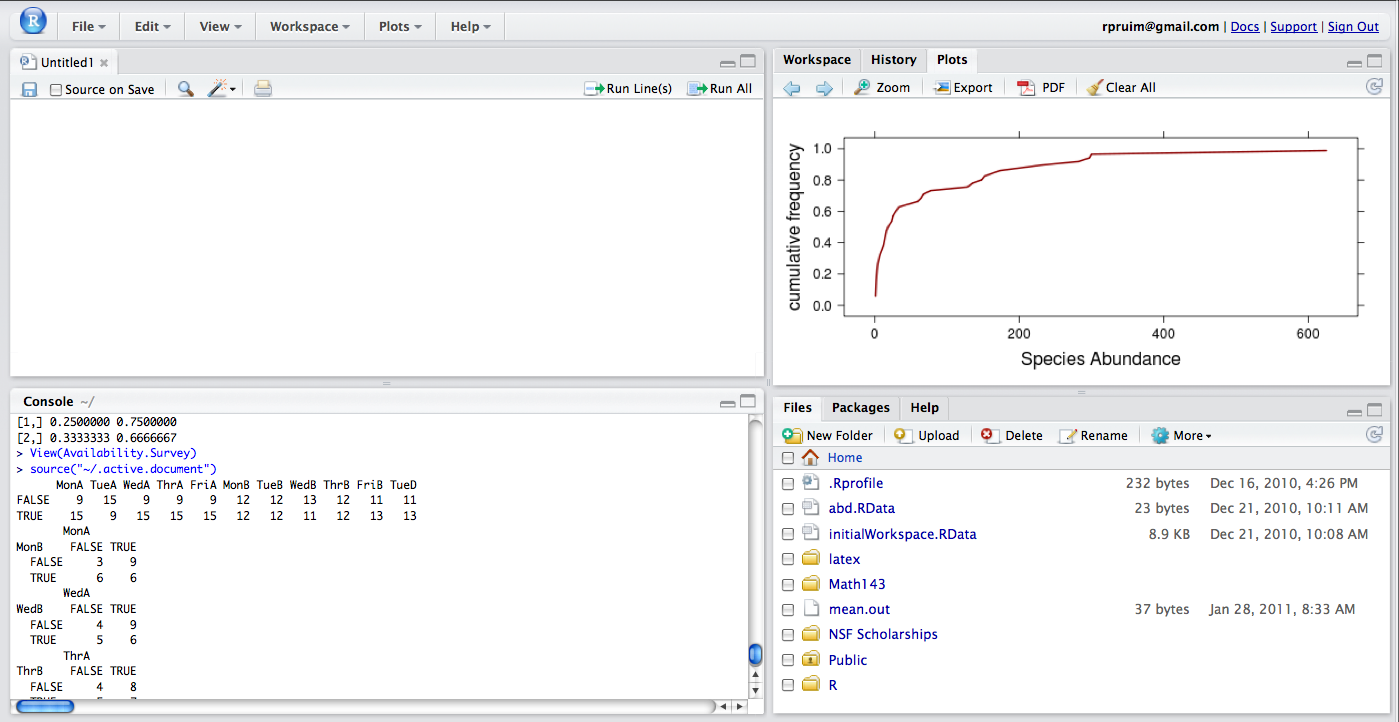
\includegraphics[width=1.0\textwidth]{images/RStudio-bigview}
\end{center}
\caption{Welcome to \Rstudio.}
\label{fig:Rstudio-bigview}%
\end{figure}

Notice that \Rstudio\ divides its world into four panels.  Several of the panels
are further subdivided into multiple tabs.
The console panel is where we type commands that \R\ will execute. 

\begin{problem}
Calculate the natural logarithm (log base $e$) and base 10 logarithm of 12,345.

What happens if you leave the comma in this number?
\begin{knitrout}
\definecolor{shadecolor}{rgb}{.97, .97, .97}{\color{fgcolor}\begin{kframe}
\begin{flushleft}
\ttfamily\noindent
\hlfunctioncall{log}\hlkeyword{(}\hlnumber{12}\hlkeyword{,}{\ }\hlnumber{345}\hlkeyword{)}\mbox{}
\normalfont
\end{flushleft}
\begin{verbatim}
[1] 0.4252
\end{verbatim}
\end{kframe}}
\end{knitrout}

%Copy-and-paste your \R\ code into your Word document.  
%Be sure to use a fixed-width font (like Courier) when you display \R\ code.  This will
%(1) make it clear that you are displaying \R\ input or output, and (2) keep things aligned 
%properly.
\end{problem}

%\pagebreak
\section{Using R as a Calculator}
\R\ can be used as a calculator.  Try typing the following commands in the console panel.

\begin{knitrout}
\definecolor{shadecolor}{rgb}{.97, .97, .97}{\color{fgcolor}\begin{kframe}
\begin{flushleft}
\ttfamily\noindent
\hlnumber{5}{\ }\hlkeyword{+}{\ }\hlnumber{3}\mbox{}
\normalfont
\end{flushleft}
\begin{verbatim}
[1] 8
\end{verbatim}
\begin{flushleft}
\ttfamily\noindent
\hlnumber{15.3}{\ }\hlkeyword{*}{\ }\hlnumber{23.4}\mbox{}
\normalfont
\end{flushleft}
\begin{verbatim}
[1] 358
\end{verbatim}
\begin{flushleft}
\ttfamily\noindent
\hlfunctioncall{sqrt}\hlkeyword{(}\hlnumber{16}\hlkeyword{)}\mbox{}
\normalfont
\end{flushleft}
\begin{verbatim}
[1] 4
\end{verbatim}
\end{kframe}}
\end{knitrout}

You can save values to named variables for later reuse.
\TeachingTip{It's probably best to settle on using 
one or the other of the right-to-left assignment operators rather than to switch
back and forth.  The authors of this document have different preferences.}%

\begin{knitrout}
\definecolor{shadecolor}{rgb}{.97, .97, .97}{\color{fgcolor}\begin{kframe}
\begin{flushleft}
\ttfamily\noindent
\hlsymbol{product}{\ }\hlassignement{=}{\ }\hlnumber{15.3}{\ }\hlkeyword{*}{\ }\hlnumber{23.4}{\ }{\ }\hlcomment{\usebox{\hlnormalsizeboxhash}{\ }save{\ }result}\hspace*{\fill}\\
\hlstd{}\hlsymbol{product}{\ }{\ }\hlcomment{\usebox{\hlnormalsizeboxhash}{\ }show{\ }the{\ }result}\mbox{}
\normalfont
\end{flushleft}
\begin{verbatim}
[1] 358
\end{verbatim}
\begin{flushleft}
\ttfamily\noindent
\hlsymbol{product}{\ }\hlassignement{\usebox{\hlnormalsizeboxlessthan}-}{\ }\hlnumber{15.3}{\ }\hlkeyword{*}{\ }\hlnumber{23.4}{\ }{\ }\hlcomment{\usebox{\hlnormalsizeboxhash}{\ }\usebox{\hlnormalsizeboxlessthan}-{\ }is{\ }assignment{\ }operator,{\ }same{\ }as{\ }=}\hspace*{\fill}\\
\hlstd{}\hlsymbol{product}\mbox{}
\normalfont
\end{flushleft}
\begin{verbatim}
[1] 358
\end{verbatim}
\begin{flushleft}
\ttfamily\noindent
\hlsymbol{newproduct}{\ }{\ }\hlcomment{\usebox{\hlnormalsizeboxhash}{\ }-\usebox{\hlnormalsizeboxgreaterthan}{\ }assigns{\ }to{\ }the{\ }right{\ }\usebox{\hlnormalsizeboxlessthan}-{\ }15.3{\ }*{\ }}\mbox{}
\normalfont
\end{flushleft}
\begin{verbatim}
Error: object 'newproduct' not found
\end{verbatim}
\begin{flushleft}
\ttfamily\noindent
{\ }{\ }{\ }{\ }\hlnumber{23.4}\mbox{}
\normalfont
\end{flushleft}
\begin{verbatim}
[1] 23.4
\end{verbatim}
\begin{flushleft}
\ttfamily\noindent
\hlsymbol{newproduct}\mbox{}
\normalfont
\end{flushleft}
\begin{verbatim}
Error: object 'newproduct' not found
\end{verbatim}
\end{kframe}}
\end{knitrout}

Once variables are defined, they can be referenced with other operators
and functions.

\begin{knitrout}
\definecolor{shadecolor}{rgb}{.97, .97, .97}{\color{fgcolor}\begin{kframe}
\begin{flushleft}
\ttfamily\noindent
\hlnumber{0.5}{\ }\hlkeyword{*}{\ }\hlsymbol{product}{\ }{\ }\hlcomment{\usebox{\hlnormalsizeboxhash}{\ }half{\ }of{\ }the{\ }product}\mbox{}
\normalfont
\end{flushleft}
\begin{verbatim}
[1] 179
\end{verbatim}
\begin{flushleft}
\ttfamily\noindent
\hlfunctioncall{log}\hlkeyword{(}\hlsymbol{product}\hlkeyword{)}{\ }{\ }\hlcomment{\usebox{\hlnormalsizeboxhash}{\ }(natural){\ }log{\ }of{\ }the{\ }product}\mbox{}
\normalfont
\end{flushleft}
\begin{verbatim}
[1] 5.881
\end{verbatim}
\begin{flushleft}
\ttfamily\noindent
\hlfunctioncall{log10}\hlkeyword{(}\hlsymbol{product}\hlkeyword{)}{\ }{\ }\hlcomment{\usebox{\hlnormalsizeboxhash}{\ }base{\ }10{\ }log{\ }of{\ }the{\ }product}\mbox{}
\normalfont
\end{flushleft}
\begin{verbatim}
[1] 2.554
\end{verbatim}
\begin{flushleft}
\ttfamily\noindent
\hlfunctioncall{log}\hlkeyword{(}\hlsymbol{product}\hlkeyword{,}{\ }\hlargument{base}{\ }\hlargument{=}{\ }\hlnumber{2}\hlkeyword{)}{\ }{\ }\hlcomment{\usebox{\hlnormalsizeboxhash}{\ }base{\ }2{\ }log{\ }of{\ }the{\ }product}\mbox{}
\normalfont
\end{flushleft}
\begin{verbatim}
[1] 8.484
\end{verbatim}
\end{kframe}}
\end{knitrout}


The semi-colon can be used to place multiple commands on one line.  
One frequent use of this is to save and print a value all in one go:

\begin{knitrout}
\definecolor{shadecolor}{rgb}{.97, .97, .97}{\color{fgcolor}\begin{kframe}
\begin{flushleft}
\ttfamily\noindent
\hlsymbol{product}{\ }\hlassignement{\usebox{\hlnormalsizeboxlessthan}-}{\ }\hlnumber{15.3}{\ }\hlkeyword{*}{\ }\hlnumber{23.4}\hspace*{\fill}\\
\hlstd{}\hlsymbol{product}{\ }{\ }\hlcomment{\usebox{\hlnormalsizeboxhash}{\ }save{\ }result{\ }and{\ }show{\ }it}\mbox{}
\normalfont
\end{flushleft}
\begin{verbatim}
[1] 358
\end{verbatim}
\end{kframe}}
\end{knitrout}



\subsection*{Four Things to Know About \R}
\begin{enumerate}
\Rwidth=6.25in
\item \R\ is case-sensitive

If you mis-capitalize something in \R\ it won't do what you want.

\item 
Functions in \R\ use the following syntax:
\begin{knitrout}
\definecolor{shadecolor}{rgb}{.97, .97, .97}{\color{fgcolor}\begin{kframe}
\begin{flushleft}
\ttfamily\noindent
\hlfunctioncall{functionname}\hlkeyword{(}\hlsymbol{argument1}\hlkeyword{,}{\ }\hlsymbol{argument2}\hlkeyword{,}{\ }\hlsymbol{...}\hlkeyword{)}\mbox{}
\normalfont
\end{flushleft}
\end{kframe}}
\end{knitrout}

\vspace{-5mm}
\TeachingTip{To help students get the hang of function arguments,
ask them \emph{What information does the computer need to compute this?}
}%
\begin{itemize}
\item The arguments are \underline{always} \emph{surrounded by (round) parentheses} and 
\emph{separated by commas}.

Some functions (like \verb!data()!) 
have no required arguments, but you still need the parentheses.

\item
If you type a function name without the parentheses, you will see the \emph{code} for that
function (this probably isn't what you want at this point).
\end{itemize}
\item
TAB completion and arrows can improve typing speed and accuracy.

If you begin a command and hit the TAB key, \R\ will show you a list of possible ways to 
complete the command.  If you hit TAB after the opening parenthesis of a function, it will show you
the list of arguments it expects.  The up and down arrows can be used to retrieve past commands.
\item
If you see a \verb!+! prompt, it means \R\ is waiting for more input.

\Caution{Your students will sometimes find themselves in a syntactic hole from which they cannot
dig out.  Teach them about the ESC key early.}%
Often this means that you have forgotten a closing parenthesis or made some other
syntax error.  If you have messed up and just want to get back to the normal plot,
hit the escape key and start the command fresh.
\end{enumerate}

\section{R Packages}

In addition to its core features, \R\ provides many more features through a (large) number 
of packages.  To use a package, it must be installed (one time), and loaded (each session).
A number of packages are already available in \Rstudio.  
The \tab{Packages} tab in \Rstudio\ will show you the list of installed packages and indicate
which of these are loaded.

\begin{center}
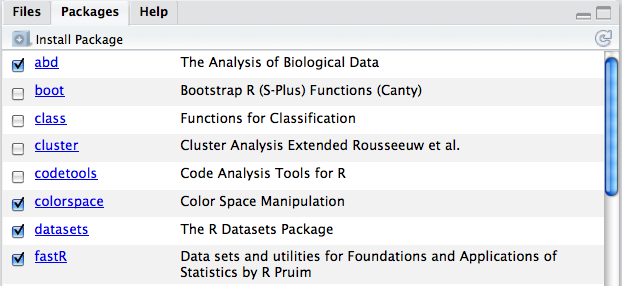
\includegraphics[width=.55\textwidth]{images/RStudio-packages}
\end{center}

%(A similar thing is true for the stand-alone versions of \R.)

Here are some packages we will use frequently:
\begin{itemize}
\item \verb!lattice!  (for graphics; this will always be installed in \R)
\item \verb!mosaic!  (for teaching statistics; this will need to be installed in \R\
from CRAN, see section \ref{sec:CRAN})
\item \verb!Hmisc!    (a package with some nice utilities; available on CRAN)
%\item \verb!vcd!      (a package for visualizing categorical data; available on CRAN)
%\item \verb!fastR!    (a package with some nice utilities; available on CRAN)
%\item \verb!abd!      (a package with some nice datasets; available on CRAN)
\end{itemize}
There are others that we use from time to time as well.  
%\verb!Hmisc!, \verb!vcd!, \verb!fastR!, \verb!abd!, and \verb!mosaic! 
\authNote{R': I think we can reduce to \verb!lattice! and \verb!mosaic!.  Possibly \verb!Hmisc!.
I'll remove dependencies on \verb!abd! as I go.}%
You should install \verb!Hmisc! and 
\verb!mosaic! the first time you use \R.
Once a package is installed, it is available to be loaded in the current or any future session.
You can install these packages 
by clicking on the ``Install Package" button in \RStudio\ and following the directions
or by using the following command:

\begin{knitrout}
\definecolor{shadecolor}{rgb}{.97, .97, .97}{\color{fgcolor}\begin{kframe}
\begin{flushleft}
\ttfamily\noindent
\hlfunctioncall{install.packages}\hlkeyword{(}\hlstring{"{}Hmisc"{}}\hlkeyword{)}{\ }{\ }\hlcomment{\usebox{\hlnormalsizeboxhash}{\ }note{\ }the{\ }quotation{\ }marks}\hspace*{\fill}\\
\hlstd{}\hlfunctioncall{install.packages}\hlkeyword{(}\hlstring{"{}mosaic"{}}\hlkeyword{)}{\ }{\ }\hlcomment{\usebox{\hlnormalsizeboxhash}{\ }note{\ }the{\ }quotation{\ }marks}\mbox{}
\normalfont
\end{flushleft}
\end{kframe}}
\end{knitrout}


Once these are installed, you can load them by checking the box in the 
\tab{Packages} tab or by using \verb!require()! (or \verb!library()!)

\begin{knitrout}
\definecolor{shadecolor}{rgb}{.97, .97, .97}{\color{fgcolor}\begin{kframe}
\begin{flushleft}
\ttfamily\noindent
\hlfunctioncall{require}\hlkeyword{(}\hlsymbol{lattice}\hlkeyword{)}{\ }{\ }\hlcomment{\usebox{\hlnormalsizeboxhash}{\ }could{\ }also{\ }use{\ }library(lattice)}\hspace*{\fill}\\
\hlstd{}\hlfunctioncall{require}\hlkeyword{(}\hlsymbol{Hmisc}\hlkeyword{)}{\ }{\ }\hlcomment{\usebox{\hlnormalsizeboxhash}{\ }do{\ }this{\ }one{\ }before{\ }mosaic}\hspace*{\fill}\\
\hlstd{}\hlfunctioncall{require}\hlkeyword{(}\hlsymbol{mosaic}\hlkeyword{)}{\ }{\ }\hlcomment{\usebox{\hlnormalsizeboxhash}{\ }do{\ }this{\ }one{\ }after{\ }Hmisc}\mbox{}
\normalfont
\end{flushleft}
\end{kframe}}
\end{knitrout}


\authNote{Add bibliography entries for books associated with packages.}
\begin{problem}
Install and load the \verb!mosaic! package.
Make sure \verb!lattice! is also loaded (no need to install it, it is already installed).

Here are some other packages you may like to install as well.
\authNote{we need fewer packages in this chapter!}
\begin{itemize}
\item
\verb!Hmisc! (Frank Harrell's miscellaneous utilities),
\item
\verb!vcd! (visualizing categorical data),
\item
\verb!fastR! (\textit{Foundations and Applications of Statistics}), and 
\item
\verb!abd! (\textit{Analysis of Biological Data}).
\end{itemize}
\end{problem}


\section{Getting Help}

If something doesn't go quite right, or if you can't remember something, it's good to know
where to turn for help.  In addition to asking your friends and neighbors, you can use
the \R\ help system.

\subsection{?}

To get help on a specific function or data set, simply precede its name with a \verb!?!:

\begin{knitrout}
\definecolor{shadecolor}{rgb}{.97, .97, .97}{\color{fgcolor}\begin{kframe}
\begin{flushleft}
\ttfamily\noindent
\hlfunctioncall{\usebox{\hlnormalsizeboxbacktick}?\usebox{\hlnormalsizeboxbacktick}}\hlkeyword{(}\hlfunctioncall{col.whitebg}\hlkeyword{(}\hlkeyword{)}\hlkeyword{)}\mbox{}
\normalfont
\end{flushleft}
\end{kframe}}
\end{knitrout}

%This will give you the documentation for the object you are interested in.

\subsection{\texttt{apropos()}}
If you don't know the exact name of a function, you can give part of the name and 
\R\ will find all functions that match.  Quotation marks are mandatory here.

\begin{knitrout}
\definecolor{shadecolor}{rgb}{.97, .97, .97}{\color{fgcolor}\begin{kframe}
\begin{flushleft}
\ttfamily\noindent
\hlfunctioncall{apropos}\hlkeyword{(}\hlstring{"{}hist"{}}\hlkeyword{)}{\ }{\ }\hlcomment{\usebox{\hlnormalsizeboxhash}{\ }must{\ }include{\ }quotes.{\ }{\ }single{\ }or{\ }double.}\mbox{}
\normalfont
\end{flushleft}
\begin{verbatim}
 [1] "event.history"              "hist"                       "hist.data.frame"           
 [4] "hist.default"               "hist.FD"                    "hist.scott"                
 [7] "histbackback"               "histogram"                  "histogram"                 
[10] "history"                    "histSpike"                  "ldahist"                   
[13] "loadhistory"                "panel.histogram"            "panel.xhistogram"          
[16] "pmfhistogram"               "prepanel.default.histogram" "savehistory"               
[19] "truehist"                   "xhistogram"                
\end{verbatim}
\end{kframe}}
\end{knitrout}


\subsection{\texttt{??} and \texttt{help.search()}}
If that fails, you can do a broader search using \verb!??! or \verb!help.search()!, 
which will find matches not only in the names of functions and data sets, 
but also in the documentation for them.  Quotations marks are optional here.

% <<help2,eval=FALSE,results=hide,echo=TRUE>>=
% ??histogram                  # any of these will work
% ??"histogram"  
% ??'histogram'  
% help.search('histogram')
% @


\subsection{Examples and Demos}

Many functions and data sets in \R\ include example code demonstrating typical uses.
For example,
\begin{knitrout}
\definecolor{shadecolor}{rgb}{.97, .97, .97}{\color{fgcolor}\begin{kframe}
\begin{flushleft}
\ttfamily\noindent
\hlfunctioncall{example}\hlkeyword{(}\hlsymbol{histogram}\hlkeyword{)}\mbox{}
\normalfont
\end{flushleft}
\end{kframe}}
\end{knitrout}

will generate a number of example plots (and provide you with the commands used to create them).
Examples such as this are intended to help you learn how specific \R\ functions work.
\FoodForThought{Not all package authors are equally skilled at creating examples.  
Some of the examples are next to useless, others are excellent.}
These examples also appear at the end of the documentation for functions and data sets.

The \verb!mosaic! package (and some other packages as well) also includes demos.  
Demos are bits of \R\ code that can be executed using the \verb!demo()! command
with the name of the demo.

To see how demos work, give this a try:
\begin{knitrout}
\definecolor{shadecolor}{rgb}{.97, .97, .97}{\color{fgcolor}\begin{kframe}
\begin{flushleft}
\ttfamily\noindent
\hlfunctioncall{demo}\hlkeyword{(}\hlsymbol{histogram}\hlkeyword{)}\mbox{}
\normalfont
\end{flushleft}
\end{kframe}}
\end{knitrout}


Demos are intended to illustrate a concept, a method, or some such thing, and are 
independent of any particular function or data set.

You can get a list of available demos using

\begin{knitrout}
\definecolor{shadecolor}{rgb}{.97, .97, .97}{\color{fgcolor}\begin{kframe}
\begin{flushleft}
\ttfamily\noindent
\hlfunctioncall{demo}\hlkeyword{(}\hlkeyword{)}{\ }{\ }\hlcomment{\usebox{\hlnormalsizeboxhash}{\ }all{\ }demos}\hspace*{\fill}\\
\hlstd{}\hlfunctioncall{demo}\hlkeyword{(}\hlargument{package}{\ }\hlargument{=}{\ }\hlstring{"{}mosaic"{}}\hlkeyword{)}{\ }{\ }\hlcomment{\usebox{\hlnormalsizeboxhash}{\ }just{\ }demos{\ }from{\ }mosaic{\ }package}\mbox{}
\normalfont
\end{flushleft}
\end{kframe}}
\end{knitrout}



\section{Data}
\subsection{Data in Packages}
Many packages contain data sets.  You can see a list of all data sets in all loaded packages
using 

\begin{knitrout}
\definecolor{shadecolor}{rgb}{.97, .97, .97}{\color{fgcolor}\begin{kframe}
\begin{flushleft}
\ttfamily\noindent
\hlfunctioncall{data}\hlkeyword{(}\hlkeyword{)}\mbox{}
\normalfont
\end{flushleft}
\end{kframe}}
\end{knitrout}


Typically (provide the author of the package allowed for lazy loading of data) 
you can use data sets by simply typing their names.  But if you have already
used that name for something or need to refresh the data after making some changes you no longer
want, you can explicitly load the data using the \verb!data()! function with the name of the 
data set you want.

\begin{knitrout}
\definecolor{shadecolor}{rgb}{.97, .97, .97}{\color{fgcolor}\begin{kframe}
\begin{flushleft}
\ttfamily\noindent
\hlfunctioncall{data}\hlkeyword{(}\hlsymbol{iris}\hlkeyword{)}\mbox{}
\normalfont
\end{flushleft}
\end{kframe}}
\end{knitrout}


\subsection{Data Frames}

Data sets are usually stored in a special structure called a \term{data frame}.

\begin{boxedText}
Data frames have a 2-dimensional structure.  
\medskip
\begin{itemize}
\item 
Rows correspond to 
\term{observational units} (people, animals, plants, or other objects we
are collecting data about).
\item
Columns correspond to \term{variables} (measurements collected on each 
observational unit).
\end{itemize}
\end{boxedText}

We'll talk later about how to get your own data into \R.  For now we'll use 
some data that comes with \R\ and is all ready for you to use.
The \verb!iris! data frame contains 5 \term{variables} measured for each
of 150 iris plants (the observational units).  
The \verb!iris! data set is included with the default \R\ installation.  
(Technically, it is located in a package called \verb!datasets!  which is always available.)

There are several ways we can get some idea about what is in the \verb!iris! data frame.

\begin{knitrout}
\definecolor{shadecolor}{rgb}{.97, .97, .97}{\color{fgcolor}\begin{kframe}
\begin{flushleft}
\ttfamily\noindent
\hlfunctioncall{str}\hlkeyword{(}\hlsymbol{iris}\hlkeyword{)}\mbox{}
\normalfont
\end{flushleft}
\begin{verbatim}
'data.frame':	150 obs. of  5 variables:
 $ Sepal.Length: num  5.1 4.9 4.7 4.6 5 5.4 4.6 5 4.4 4.9 ...
 $ Sepal.Width : num  3.5 3 3.2 3.1 3.6 3.9 3.4 3.4 2.9 3.1 ...
 $ Petal.Length: num  1.4 1.4 1.3 1.5 1.4 1.7 1.4 1.5 1.4 1.5 ...
 $ Petal.Width : num  0.2 0.2 0.2 0.2 0.2 0.4 0.3 0.2 0.2 0.1 ...
 $ Species     : Factor w/ 3 levels "setosa","versicolor",..: 1 1 1 1 1 1 1 1 1 1 ...
\end{verbatim}
\end{kframe}}
\end{knitrout}


\begin{knitrout}
\definecolor{shadecolor}{rgb}{.97, .97, .97}{\color{fgcolor}\begin{kframe}
\begin{flushleft}
\ttfamily\noindent
\hlfunctioncall{summary}\hlkeyword{(}\hlsymbol{iris}\hlkeyword{)}\mbox{}
\normalfont
\end{flushleft}
\begin{verbatim}
  Sepal.Length   Sepal.Width    Petal.Length   Petal.Width        Species  
 Min.   :4.30   Min.   :2.00   Min.   :1.00   Min.   :0.1   setosa    :50  
 1st Qu.:5.10   1st Qu.:2.80   1st Qu.:1.60   1st Qu.:0.3   versicolor:50  
 Median :5.80   Median :3.00   Median :4.35   Median :1.3   virginica :50  
 Mean   :5.84   Mean   :3.06   Mean   :3.76   Mean   :1.2                  
 3rd Qu.:6.40   3rd Qu.:3.30   3rd Qu.:5.10   3rd Qu.:1.8                  
 Max.   :7.90   Max.   :4.40   Max.   :6.90   Max.   :2.5                  
\end{verbatim}
\end{kframe}}
\end{knitrout}


\begin{knitrout}
\definecolor{shadecolor}{rgb}{.97, .97, .97}{\color{fgcolor}\begin{kframe}
\begin{flushleft}
\ttfamily\noindent
\hlfunctioncall{head}\hlkeyword{(}\hlsymbol{iris}\hlkeyword{)}\mbox{}
\normalfont
\end{flushleft}
\begin{verbatim}
  Sepal.Length Sepal.Width Petal.Length Petal.Width Species
1          5.1         3.5          1.4         0.2  setosa
2          4.9         3.0          1.4         0.2  setosa
3          4.7         3.2          1.3         0.2  setosa
4          4.6         3.1          1.5         0.2  setosa
5          5.0         3.6          1.4         0.2  setosa
6          5.4         3.9          1.7         0.4  setosa
\end{verbatim}
\end{kframe}}
\end{knitrout}

In interactive mode, you can also try
\begin{knitrout}
\definecolor{shadecolor}{rgb}{.97, .97, .97}{\color{fgcolor}\begin{kframe}
\begin{flushleft}
\ttfamily\noindent
\hlfunctioncall{View}\hlkeyword{(}\hlsymbol{iris}\hlkeyword{)}\mbox{}
\normalfont
\end{flushleft}
\end{kframe}}
\end{knitrout}

to see the data or 
\begin{knitrout}
\definecolor{shadecolor}{rgb}{.97, .97, .97}{\color{fgcolor}\begin{kframe}
\begin{flushleft}
\ttfamily\noindent
\hlfunctioncall{\usebox{\hlnormalsizeboxbacktick}?\usebox{\hlnormalsizeboxbacktick}}\hlkeyword{(}\hlsymbol{iris}\hlkeyword{)}\mbox{}
\normalfont
\end{flushleft}
\end{kframe}}
\end{knitrout}

to get the documentation about for the data set.

%\subsection{Getting at the Variables}
Access to an individual variable in a data frame uses the \verb!$! operator in
the following syntax:

\begin{knitrout}
\definecolor{shadecolor}{rgb}{.97, .97, .97}{\color{fgcolor}\begin{kframe}
\begin{flushleft}
\ttfamily\noindent
\hlsymbol{dataframe}\hlkeyword{\usebox{\hlnormalsizeboxdollar}}\hlsymbol{variable}\mbox{}
\normalfont
\end{flushleft}
\end{kframe}}
\end{knitrout}

or 
\begin{knitrout}
\definecolor{shadecolor}{rgb}{.97, .97, .97}{\color{fgcolor}\begin{kframe}
\begin{flushleft}
\ttfamily\noindent
\hlfunctioncall{with}\hlkeyword{(}\hlsymbol{dataframe}\hlkeyword{,}{\ }\hlsymbol{variable}\hlkeyword{)}\mbox{}
\normalfont
\end{flushleft}
\end{kframe}}
\end{knitrout}


For example, either of 

\begin{knitrout}
\definecolor{shadecolor}{rgb}{.97, .97, .97}{\color{fgcolor}\begin{kframe}
\begin{flushleft}
\ttfamily\noindent
\hlsymbol{iris}\hlkeyword{\usebox{\hlnormalsizeboxdollar}}\hlsymbol{Sepal.Length}\mbox{}
\normalfont
\end{flushleft}
\end{kframe}}
\end{knitrout}

or 
\begin{knitrout}
\definecolor{shadecolor}{rgb}{.97, .97, .97}{\color{fgcolor}\begin{kframe}
\begin{flushleft}
\ttfamily\noindent
\hlfunctioncall{with}\hlkeyword{(}\hlsymbol{iris}\hlkeyword{,}{\ }\hlsymbol{Sepal.Length}\hlkeyword{)}\mbox{}
\normalfont
\end{flushleft}
\end{kframe}}
\end{knitrout}

shows the contents of the \verb!Sepal.Length! variable in the following format.
\begin{knitrout}
\definecolor{shadecolor}{rgb}{.97, .97, .97}{\color{fgcolor}\begin{kframe}
\begin{verbatim}
  [1] 5.1 4.9 4.7 4.6 5.0 5.4 4.6 5.0 4.4 4.9 5.4 4.8 4.8 4.3 5.8 5.7 5.4 5.1 5.7 5.1 5.4 5.1 4.6
 [24] 5.1 4.8 5.0 5.0 5.2 5.2 4.7 4.8 5.4 5.2 5.5 4.9 5.0 5.5 4.9 4.4 5.1 5.0 4.5 4.4 5.0 5.1 4.8
 [47] 5.1 4.6 5.3 5.0 7.0 6.4 6.9 5.5 6.5 5.7 6.3 4.9 6.6 5.2 5.0 5.9 6.0 6.1 5.6 6.7 5.6 5.8 6.2
 [70] 5.6 5.9 6.1 6.3 6.1 6.4 6.6 6.8 6.7 6.0 5.7 5.5 5.5 5.8 6.0 5.4 6.0 6.7 6.3 5.6 5.5 5.5 6.1
 [93] 5.8 5.0 5.6 5.7 5.7 6.2 5.1 5.7 6.3 5.8 7.1 6.3 6.5 7.6 4.9 7.3 6.7 7.2 6.5 6.4 6.8 5.7 5.8
[116] 6.4 6.5 7.7 7.7 6.0 6.9 5.6 7.7 6.3 6.7 7.2 6.2 6.1 6.4 7.2 7.4 7.9 6.4 6.3 6.1 7.7 6.3 6.4
[139] 6.0 6.9 6.7 6.9 5.8 6.8 6.7 6.7 6.3 6.5 6.2 5.9
\end{verbatim}
\end{kframe}}
\end{knitrout}


But this isn't very useful for a large data set.  
We would prefer to compute numerical or graphical summaries.  We'll do that shortly.

The \verb!attach()! function in R can be used to make objects within dataframes
accessible in R with fewer keystrokes, but we strongly discourage its use, as
it often leads to name conflicts.  
\Caution{Avoid the use of \function{attach()}.}
The Google R Style Guide
(\url{http://google-styleguide.googlecode.com/svn/trunk/google-r-style.html})
echoes this advice, stating that \emph{The possibilities for creating errors
when using attach are numerous. Avoid it.} 
It is far better to directly access
variables using the \verb!\$! syntax or to use the \function{with()} function.

\subsection{Using Your Own Data}
\Rstudio\ will help you import your own data.  To do so use the ``Import Dataset" 
button in the \tab{Workspace} tab.  You can load data from text files, from the web, or from
google spreadsheets.   

%\subsubsection*{From Google Spreadsheets}

\textbf{From Google.}
The easiest of these is the Google spreadsheets option: Just click, select
your spreadsheet, choose a name, and you're done.

%\subsubsection*{From Excel}
\textbf{From Excel},
you need to follow a 3-step process:
\begin{enumerate}
\item
Save your Excel worksheet as a csv (comma separated value) file.
\item
Upload (in the \tab{Files} tab) your csv file to the server, where you can create folders and store
files in your personal account.  
(To share things with others: Put the files in your Public folder.  
Read the\texttt{AboutPublic.txt} file in that folder for directions.)
\item
Now import ``from a text file'' in the \tab{Workspace} tab.
\end{enumerate}

In either case, be sure to do the following:
\begin{itemize}
\item Choose good variables names.
\item Put your variables names in the first row.
\item Use each subsequent row for one observational unit.
\item Give the resulting data frame a good name.
\end{itemize}
\authNoted{I moved Danny's Simple Relational Database suggestion
to \ref{sec:manipulatingData}.
I don't think I would use a grade/courses example for students nor that
I would introduce \function{merge()} \emph{et al} to newbies right away.
My goal was to have this appendix look like something that I would give
to students as is in the first week.
In any case, I agree that we should have a section on this somewhere.
[RJP]
}%

If you are not using \RStudio, you can read files using
\function{read.csv()} or \function{read.table()} (for white space delimited files).
The \function{mosaic} package includes a function called \function{read.file()} that uses 
slightly different default settings and infers whether it should use \function{read.csv()},
\function{read.table()}, or \function{load()} based on the file name.  
\DiggingDeeper[\centerline{\function{load()}}]{\function{load()} is used
for opening files that store \R\ objects in `native' format.}

Each of these functions 
also accepts a URL in place of a file name, which provides an easy way to distribute data
via the Internet:
\begin{knitrout}
\definecolor{shadecolor}{rgb}{.97, .97, .97}{\color{fgcolor}\begin{kframe}
\begin{flushleft}
\ttfamily\noindent
\hlsymbol{births}{\ }\hlassignement{\usebox{\hlnormalsizeboxlessthan}-}{\ }\hlfunctioncall{read.table}\hlkeyword{(}\hlstring{"{}http://www.calvin.edu/\urltilda{}rpruim/data/births.txt"{}}\hlkeyword{,}\hspace*{\fill}\\
\hlstd{}{\ }{\ }{\ }{\ }\hlargument{header}{\ }\hlargument{=}{\ }\hlnumber{TRUE}\hlkeyword{)}\hspace*{\fill}\\
\hlstd{}\hlfunctioncall{head}\hlkeyword{(}\hlsymbol{births}\hlkeyword{)}{\ }{\ }\hlcomment{\usebox{\hlnormalsizeboxhash}{\ }number{\ }of{\ }live{\ }births{\ }in{\ }the{\ }US{\ }each{\ }day{\ }of{\ }1978.}\mbox{}
\normalfont
\end{flushleft}
\begin{verbatim}
    date births datenum dayofyear
1 1/1/78   7701    6575         1
2 1/2/78   7527    6576         2
3 1/3/78   8825    6577         3
4 1/4/78   8859    6578         4
5 1/5/78   9043    6579         5
6 1/6/78   9208    6580         6
\end{verbatim}
\end{kframe}}
\end{knitrout}

The \pkg{mosaic} package provides \function{read.file()} which attempts to infer
the file type from its extension and then applies 
\function{read.csv()}, \function{read.table()}, or \function{load()}.
\begin{knitrout}
\definecolor{shadecolor}{rgb}{.97, .97, .97}{\color{fgcolor}\begin{kframe}
\begin{flushleft}
\ttfamily\noindent
\hlsymbol{births}{\ }\hlassignement{\usebox{\hlnormalsizeboxlessthan}-}{\ }\hlfunctioncall{read.file}\hlkeyword{(}\hlstring{"{}http://www.calvin.edu/\urltilda{}rpruim/data/births.txt"{}}\hlkeyword{)}\mbox{}
\normalfont
\end{flushleft}
\end{kframe}}
\end{knitrout}

It also sets a number of defaults, including \option{header=TRUE}.

\begin{problem}
Enter the following small data set in an Excel or Google spreadsheet and import the 
data into \Rstudio.

\begin{center}
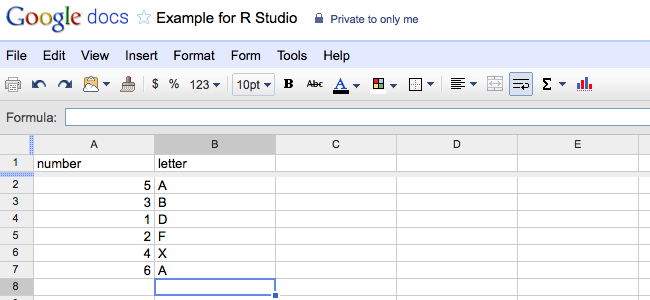
\includegraphics[width=.5\textwidth]{images/GoogleSpreadsheet}
\end{center}

You can import directly from Google.  From Excel, save the file as a csv and
import that (as a text file) into \Rstudio.  Name the data frame \texttt{JunkData}.
\end{problem}

\subsection{Putting Data Into a Package}

It is not that difficult to take a collection of csv files (a format available for many books)
and put them all into a package.
The \verb!abd! package contains data sets from \textit{The Analysis of Biological Data}, for example.  
Kevin Middleton and Randall Pruim contacted the authors and obtained permission to 
build and disseminate this package.

The \verb!abdData()! function in \verb!abd! makes it easy to map examples and exercises in that book to 
data frame names in the \verb!abd! package.

\begin{knitrout}
\definecolor{shadecolor}{rgb}{.97, .97, .97}{\color{fgcolor}\begin{kframe}
\begin{flushleft}
\ttfamily\noindent
\hlfunctioncall{abdData}\hlkeyword{(}\hlstring{"{}human"{}}\hlkeyword{)}{\ }{\ }\hlcomment{\usebox{\hlnormalsizeboxhash}{\ }all{\ }data{\ }sets{\ }with{\ }\usebox{\hlnormalsizeboxsinglequote}human\usebox{\hlnormalsizeboxsinglequote}{\ }in{\ }the{\ }name}\mbox{}
\normalfont
\end{flushleft}
\begin{verbatim}
Error: could not find function "abdData"
\end{verbatim}
\end{kframe}}
\end{knitrout}


\begin{knitrout}
\definecolor{shadecolor}{rgb}{.97, .97, .97}{\color{fgcolor}\begin{kframe}
\begin{flushleft}
\ttfamily\noindent
\hlfunctioncall{abdData}\hlkeyword{(}\hlnumber{2}\hlkeyword{)}{\ }{\ }\hlcomment{\usebox{\hlnormalsizeboxhash}{\ }all{\ }data{\ }sets{\ }in{\ }chapter{\ }2}\mbox{}
\normalfont
\end{flushleft}
\begin{verbatim}
Error: could not find function "abdData"
\end{verbatim}
\end{kframe}}
\end{knitrout}


For information on how to create such packages, consult the \textit{Writing R Extensions} manual
on CRAN.

\section{Summarizing Data}

\subsection{A Few Numerical Summaries}
\R\ includes functions that compute a wide range of numerical and graphical summaries.  
Most of the numerical summaries already familiar to you have obvious names.  
Here are a few examples.  
%(If you don't know what some of these -- like IQR -- are, don't worry;
%we'll be discussing them soon.)

\begin{knitrout}
\definecolor{shadecolor}{rgb}{.97, .97, .97}{\color{fgcolor}\begin{kframe}
\begin{flushleft}
\ttfamily\noindent
\hlfunctioncall{with}\hlkeyword{(}\hlsymbol{iris}\hlkeyword{,}{\ }\hlfunctioncall{mean}\hlkeyword{(}\hlsymbol{Sepal.Length}\hlkeyword{)}\hlkeyword{)}{\ }{\ }\hlcomment{\usebox{\hlnormalsizeboxhash}{\ }or{\ }mean(iris\usebox{\hlnormalsizeboxdollar}Sepal.Length)}\mbox{}
\normalfont
\end{flushleft}
\begin{verbatim}
 mean 
5.843 
\end{verbatim}
\begin{flushleft}
\ttfamily\noindent
\hlfunctioncall{with}\hlkeyword{(}\hlsymbol{iris}\hlkeyword{,}{\ }\hlfunctioncall{median}\hlkeyword{(}\hlsymbol{Sepal.Length}\hlkeyword{)}\hlkeyword{)}{\ }{\ }\hlcomment{\usebox{\hlnormalsizeboxhash}{\ }or{\ }median(iris\usebox{\hlnormalsizeboxdollar}Sepal.Length)}\mbox{}
\normalfont
\end{flushleft}
\begin{verbatim}
median 
   5.8 
\end{verbatim}
\begin{flushleft}
\ttfamily\noindent
\hlfunctioncall{with}\hlkeyword{(}\hlsymbol{iris}\hlkeyword{,}{\ }\hlfunctioncall{sd}\hlkeyword{(}\hlsymbol{Sepal.Length}\hlkeyword{)}\hlkeyword{)}{\ }{\ }\hlcomment{\usebox{\hlnormalsizeboxhash}{\ }or{\ }sd(iris\usebox{\hlnormalsizeboxdollar}Sepal.Length)}\mbox{}
\normalfont
\end{flushleft}
\begin{verbatim}
    sd 
0.8281 
\end{verbatim}
\begin{flushleft}
\ttfamily\noindent
\hlfunctioncall{with}\hlkeyword{(}\hlsymbol{iris}\hlkeyword{,}{\ }\hlfunctioncall{quantile}\hlkeyword{(}\hlsymbol{Sepal.Length}\hlkeyword{)}\hlkeyword{)}{\ }{\ }\hlcomment{\usebox{\hlnormalsizeboxhash}{\ }or{\ }quantile(iris\usebox{\hlnormalsizeboxdollar}Sepal.Length)}\mbox{}
\normalfont
\end{flushleft}
\begin{verbatim}
  0%  25%  50%  75% 100% 
 4.3  5.1  5.8  6.4  7.9 
\end{verbatim}
\begin{flushleft}
\ttfamily\noindent
\hlfunctioncall{with}\hlkeyword{(}\hlsymbol{iris}\hlkeyword{,}{\ }\hlfunctioncall{IQR}\hlkeyword{(}\hlsymbol{Sepal.Length}\hlkeyword{)}\hlkeyword{)}{\ }{\ }\hlcomment{\usebox{\hlnormalsizeboxhash}{\ }or{\ }IQR(iris\usebox{\hlnormalsizeboxdollar}Sepal.Length)}\mbox{}
\normalfont
\end{flushleft}
\begin{verbatim}
[1] 1.3
\end{verbatim}
\begin{flushleft}
\ttfamily\noindent
\hlfunctioncall{IQR}\hlkeyword{(}\hlsymbol{iris}\hlkeyword{\usebox{\hlnormalsizeboxdollar}}\hlsymbol{Sepal.Length}\hlkeyword{)}\mbox{}
\normalfont
\end{flushleft}
\begin{verbatim}
[1] 1.3
\end{verbatim}
\end{kframe}}
\end{knitrout}


The \verb!favstats()! function in the \verb!mosaic! package computes several numerical 
summaries all at once.

\begin{knitrout}
\definecolor{shadecolor}{rgb}{.97, .97, .97}{\color{fgcolor}\begin{kframe}
\begin{flushleft}
\ttfamily\noindent
\hlfunctioncall{require}\hlkeyword{(}\hlsymbol{mosaic}\hlkeyword{)}{\ }{\ }\hlcomment{\usebox{\hlnormalsizeboxhash}{\ }if{\ }you{\ }haven\usebox{\hlnormalsizeboxsinglequote}t{\ }already{\ }loaded{\ }the{\ }mosaic{\ }package}\hspace*{\fill}\\
\hlstd{}\hlfunctioncall{favstats}\hlkeyword{(}\hlsymbol{iris}\hlkeyword{\usebox{\hlnormalsizeboxdollar}}\hlsymbol{Sepal.Length}\hlkeyword{)}\mbox{}
\normalfont
\end{flushleft}
\begin{verbatim}
    0%    25%    50%    75%   100%   mean     sd    var 
4.3000 5.1000 5.8000 6.4000 7.9000 5.8433 0.8281 0.6857 
\end{verbatim}
\end{kframe}}
\end{knitrout}


Here's something a little fancier.

\begin{knitrout}
\definecolor{shadecolor}{rgb}{.97, .97, .97}{\color{fgcolor}\begin{kframe}
\begin{flushleft}
\ttfamily\noindent
\hlfunctioncall{require}\hlkeyword{(}\hlsymbol{Hmisc}\hlkeyword{)}\hspace*{\fill}\\
\hlstd{}\hlfunctioncall{summary}\hlkeyword{(}\hlsymbol{Sepal.Length}{\ }\hlkeyword{\urltilda{}}{\ }\hlsymbol{Species}\hlkeyword{,}{\ }\hlargument{data}{\ }\hlargument{=}{\ }\hlsymbol{iris}\hlkeyword{,}{\ }\hlargument{fun}{\ }\hlargument{=}{\ }\hlsymbol{favstats}\hlkeyword{)}\mbox{}
\normalfont
\end{flushleft}
\begin{verbatim}
Sepal.Length    N=150

+-------+----------+---+---+-----+---+---+----+-----+------+------+
|       |          |N  |0% |25%  |50%|75%|100%|mean |sd    |var   |
+-------+----------+---+---+-----+---+---+----+-----+------+------+
|Species|setosa    | 50|4.3|4.800|5.0|5.2|5.8 |5.006|0.3525|0.1242|
|       |versicolor| 50|4.9|5.600|5.9|6.3|7.0 |5.936|0.5162|0.2664|
|       |virginica | 50|4.9|6.225|6.5|6.9|7.9 |6.588|0.6359|0.4043|
+-------+----------+---+---+-----+---+---+----+-----+------+------+
|Overall|          |150|4.3|5.100|5.8|6.4|7.9 |5.843|0.8281|0.6857|
+-------+----------+---+---+-----+---+---+----+-----+------+------+
\end{verbatim}
\end{kframe}}
\end{knitrout}

(Note: This requires installation of the \verb!Hmisc! package.)

\begin{problem}
What is the average (mean) \emph{width} of the sepals in the \verb!iris! data set?
\end{problem}

\begin{problem}
Determine the average (mean) sepal width for each of the three species in the \verb!iris! data set.
\end{problem}

\subsection{Lattice Graphics}

There are several ways to make graphs in \R.  One approach is a system called
\verb!lattice! graphics.  The first step for using \verb!lattice! is to
load the \verb!lattice! package using the check box in the \tab{Packages} tab or using
the following command:

\begin{knitrout}
\definecolor{shadecolor}{rgb}{.97, .97, .97}{\color{fgcolor}\begin{kframe}
\begin{flushleft}
\ttfamily\noindent
\hlfunctioncall{require}\hlkeyword{(}\hlsymbol{lattice}\hlkeyword{)}\mbox{}
\normalfont
\end{flushleft}
\end{kframe}}
\end{knitrout}

\verb!lattice! plots make use of a \term{formula interface}:

\begin{knitrout}
\definecolor{shadecolor}{rgb}{.97, .97, .97}{\color{fgcolor}\begin{kframe}
\begin{flushleft}
\ttfamily\noindent
\hlfunctioncall{plotname}\hlkeyword{(}\hlsymbol{y}{\ }\hlkeyword{\urltilda{}}{\ }\hlsymbol{x}{\ }\hlkeyword{|}{\ }\hlsymbol{z}\hlkeyword{,}{\ }\hlargument{data}{\ }\hlargument{=}{\ }\hlsymbol{dataname}\hlkeyword{,}{\ }\hlargument{groups}{\ }\hlargument{=}{\ }\hlsymbol{grouping\usebox{\hlnormalsizeboxunderscore}variable}\hlkeyword{,}\hspace*{\fill}\\
\hlstd{}{\ }{\ }{\ }{\ }\hlsymbol{...}\hlkeyword{)}\mbox{}
\normalfont
\end{flushleft}
\end{kframe}}
\end{knitrout}

\begin{itemize}
\item
Here are the names of several \verb!lattice! plots:
\begin{itemize}
\item \verb!dotPlot! (notice the capital P; \verb!dotplot()! does something different)
\footnote{\texttt{dotPlot()} is in the \texttt{mosaic} package and was created because \texttt{dotplot()} in
the \texttt{lattice} package makes something different from what we call a dot plot.}
\item \verb!histogram!  (for histograms)
\item \verb!bwplot!  (for boxplots)
\item \verb!xyplot!  (for scatter plots)
\item \verb!qqmath!  (for quantile-quantile plots)
\end{itemize}
\item
\verb!x! is the name of the variable that is plotted along the horizontal 
($x$) axis.
\item
\verb!y! is the name of the variable that is plotted along the vertical ($y$) 
axis.  (For some plots, this slot is empty because \R\ computes these values
from the values of \verb!x!.)
\item
\verb!z! is a conditioning variable used to split the plot into 
multiple subplots called \term{panels}.
\item
\verb!grouping_variable! is used to display different groups differently
(different colors or symbols, for example) within the same panel.
\item
\verb!...! There are many additional arguments to these functions that let you
control just how the plots look.  (But we'll focus on the basics for now.)
\end{itemize}

%\subsection*{Some Examples}

\subsection{Dot plots: \texttt{dotPlot()}}

A dot plot represents each value of a quantitative variable with a dot.  The values
are rounded a bit so that the dots line up neatly, and dots are stacked up into little
towers when the data values cluster near each other.

For a dot plot, the \verb!y! component of the formula is empty since we let \R\
calculate that for us.

\begin{knitrout}
\definecolor{shadecolor}{rgb}{.97, .97, .97}{\color{fgcolor}\begin{kframe}
\begin{flushleft}
\ttfamily\noindent
\hlcomment{\usebox{\hlnormalsizeboxhash}{\ }was{\ }dotPlot}\hspace*{\fill}\\
\hlstd{}\hlfunctioncall{histogram}\hlkeyword{(}\hlkeyword{\urltilda{}}\hlsymbol{Sepal.Length}\hlkeyword{,}{\ }\hlargument{data}{\ }\hlargument{=}{\ }\hlsymbol{iris}\hlkeyword{,}{\ }\hlargument{n}{\ }\hlargument{=}{\ }\hlnumber{20}\hlkeyword{)}{\ }{\ }\hlcomment{\usebox{\hlnormalsizeboxhash}{\ }n=20{\ }gives{\ }us{\ }approximately{\ }20{\ }towers}\mbox{}
\normalfont
\end{flushleft}


\centering{}\includegraphics{figures/fig-iris-dotPlot} 

\end{kframe}}
\end{knitrout}

We can use a conditional variable to give us separate dot plots for each species.

\begin{knitrout}
\definecolor{shadecolor}{rgb}{.97, .97, .97}{\color{fgcolor}\begin{kframe}
\begin{flushleft}
\ttfamily\noindent
\hlcomment{\usebox{\hlnormalsizeboxhash}{\ }was{\ }dotPlot}\hspace*{\fill}\\
\hlstd{}\hlfunctioncall{histogram}\hlkeyword{(}\hlkeyword{\urltilda{}}\hlsymbol{Sepal.Length}{\ }\hlkeyword{|}{\ }\hlsymbol{Species}\hlkeyword{,}{\ }\hlargument{data}{\ }\hlargument{=}{\ }\hlsymbol{iris}\hlkeyword{,}{\ }\hlargument{n}{\ }\hlargument{=}{\ }\hlnumber{20}\hlkeyword{)}\mbox{}
\normalfont
\end{flushleft}
\end{kframe}}
\end{knitrout}

\begin{knitrout}
\definecolor{shadecolor}{rgb}{.97, .97, .97}{\color{fgcolor}\begin{kframe}


\centering{}\includegraphics{figures/fig-iris-dotPlot-condB} 

\end{kframe}}
\end{knitrout}


\subsection{Histograms: \texttt{histogram()}}

Histograms are a lot like dot plots, but the towers of dots are replaced by a vertical bar.
Again the \verb!y! component of the formula is empty since we let \R\
compute the heights of the bars for us.
\begin{knitrout}
\definecolor{shadecolor}{rgb}{.97, .97, .97}{\color{fgcolor}\begin{kframe}
\begin{flushleft}
\ttfamily\noindent
\hlfunctioncall{histogram}\hlkeyword{(}\hlkeyword{\urltilda{}}\hlsymbol{Sepal.Length}\hlkeyword{,}{\ }\hlargument{data}{\ }\hlargument{=}{\ }\hlsymbol{iris}\hlkeyword{,}{\ }\hlargument{n}{\ }\hlargument{=}{\ }\hlnumber{20}\hlkeyword{)}{\ }{\ }\hlcomment{\usebox{\hlnormalsizeboxhash}{\ }n={\ }20{\ }gives{\ }approx.{\ }20{\ }bars}\mbox{}
\normalfont
\end{flushleft}


\centering{}\includegraphics{figures/fig-iris-histogram} 

\end{kframe}}
\end{knitrout}

We can use a conditional variable to give us separate histograms for each species.

\begin{knitrout}
\definecolor{shadecolor}{rgb}{.97, .97, .97}{\color{fgcolor}\begin{kframe}
\begin{flushleft}
\ttfamily\noindent
\hlfunctioncall{histogram}\hlkeyword{(}\hlkeyword{\urltilda{}}\hlsymbol{Sepal.Length}{\ }\hlkeyword{|}{\ }\hlsymbol{Species}\hlkeyword{,}{\ }\hlargument{data}{\ }\hlargument{=}{\ }\hlsymbol{iris}\hlkeyword{,}{\ }\hlargument{n}{\ }\hlargument{=}{\ }\hlnumber{20}\hlkeyword{)}\mbox{}
\normalfont
\end{flushleft}


\centering{}\includegraphics{figures/fig-iris-histogram-cond} 

\end{kframe}}
\end{knitrout}



In lattice lingo, the three subplots are called panels and the 
labels at the top are called strips.  (Strips can be placed on the left side if you 
prefer.)


\subsection{Boxplots:  \texttt{bwplot()}}

Boxplots are made pretty much the same way as histograms:
\begin{knitrout}
\definecolor{shadecolor}{rgb}{.97, .97, .97}{\color{fgcolor}\begin{kframe}
\begin{flushleft}
\ttfamily\noindent
\hlfunctioncall{bwplot}\hlkeyword{(}\hlkeyword{\urltilda{}}\hlsymbol{Sepal.Length}\hlkeyword{,}{\ }\hlargument{data}{\ }\hlargument{=}{\ }\hlsymbol{iris}\hlkeyword{)}\mbox{}
\normalfont
\end{flushleft}


\centering{}\includegraphics{figures/fig-iris-bwplot} 

\end{kframe}}
\end{knitrout}


We can use conditioning as we did for histograms:

\begin{knitrout}
\definecolor{shadecolor}{rgb}{.97, .97, .97}{\color{fgcolor}\begin{kframe}
\begin{flushleft}
\ttfamily\noindent
\hlfunctioncall{bwplot}\hlkeyword{(}\hlkeyword{\urltilda{}}\hlsymbol{Sepal.Length}{\ }\hlkeyword{|}{\ }\hlsymbol{Species}\hlkeyword{,}{\ }\hlargument{data}{\ }\hlargument{=}{\ }\hlsymbol{iris}\hlkeyword{)}\mbox{}
\normalfont
\end{flushleft}


\centering{}\includegraphics{figures/fig-iris-bwplot-cond} 

\end{kframe}}
\end{knitrout}


\vspace{-8mm}

But there are better ways to do this.
\begin{knitrout}
\definecolor{shadecolor}{rgb}{.97, .97, .97}{\color{fgcolor}\begin{kframe}
\begin{flushleft}
\ttfamily\noindent
\hlfunctioncall{bwplot}\hlkeyword{(}\hlsymbol{Sepal.Length}{\ }\hlkeyword{\urltilda{}}{\ }\hlsymbol{Species}\hlkeyword{,}{\ }\hlargument{data}{\ }\hlargument{=}{\ }\hlsymbol{iris}\hlkeyword{)}\mbox{}
\normalfont
\end{flushleft}


\centering{}\includegraphics{figures/fig-iris-bwplot-2d} 

\end{kframe}}
\end{knitrout}

This is improved, but the species names run into each other.
We could fix that run-together text by using abbreviated names or rotating the
labels 45 or 90 degrees.  Instead of those solutions, we can also just reverse the roles
of the horizontal and vertical axes.
\begin{knitrout}
\definecolor{shadecolor}{rgb}{.97, .97, .97}{\color{fgcolor}\begin{kframe}
\begin{flushleft}
\ttfamily\noindent
\hlfunctioncall{bwplot}\hlkeyword{(}\hlsymbol{Species}{\ }\hlkeyword{\urltilda{}}{\ }\hlsymbol{Sepal.Length}\hlkeyword{,}{\ }\hlargument{data}{\ }\hlargument{=}{\ }\hlsymbol{iris}\hlkeyword{)}\mbox{}
\normalfont
\end{flushleft}


\centering{}\includegraphics{figures/fig-iris-bwplot-2dh} 

\end{kframe}}
\end{knitrout}


\vspace{-12mm}

%\pagebreak

\subsection{Scatterplots: \texttt{xyplot()}}

Scatterplots are made with \verb!xyplot()!.  The formula interface is very natural for this.  
Just remember that the ``$y$ variable'' comes first.  (Its label is also farther left on 
the plot, if that helps you remember.)
\begin{knitrout}
\definecolor{shadecolor}{rgb}{.97, .97, .97}{\color{fgcolor}\begin{kframe}
\begin{flushleft}
\ttfamily\noindent
\hlfunctioncall{xyplot}\hlkeyword{(}\hlsymbol{Sepal.Length}{\ }\hlkeyword{\urltilda{}}{\ }\hlsymbol{Sepal.Width}\hlkeyword{,}{\ }\hlargument{data}{\ }\hlargument{=}{\ }\hlsymbol{iris}\hlkeyword{)}\mbox{}
\normalfont
\end{flushleft}


\centering{}\includegraphics{figures/fig-iris-xyplot} 

\end{kframe}}
\end{knitrout}


Again, we can use conditioning to make a panel for each species.
\begin{knitrout}
\definecolor{shadecolor}{rgb}{.97, .97, .97}{\color{fgcolor}\begin{kframe}
\begin{flushleft}
\ttfamily\noindent
\hlfunctioncall{xyplot}\hlkeyword{(}\hlsymbol{Sepal.Length}{\ }\hlkeyword{\urltilda{}}{\ }\hlsymbol{Sepal.Width}{\ }\hlkeyword{|}{\ }\hlsymbol{Species}\hlkeyword{,}{\ }\hlargument{data}{\ }\hlargument{=}{\ }\hlsymbol{iris}\hlkeyword{)}\mbox{}
\normalfont
\end{flushleft}


\centering{}\includegraphics{figures/fig-iris-xyplot-cond} 

\end{kframe}}
\end{knitrout}



Even better (for this example), we can use the \verb!groups! argument to indicate the different species using
different symbols on the same panel.
\begin{knitrout}
\definecolor{shadecolor}{rgb}{.97, .97, .97}{\color{fgcolor}\begin{kframe}
\begin{flushleft}
\ttfamily\noindent
\hlfunctioncall{xyplot}\hlkeyword{(}\hlsymbol{Sepal.Length}{\ }\hlkeyword{\urltilda{}}{\ }\hlsymbol{Sepal.Width}\hlkeyword{,}{\ }\hlargument{groups}{\ }\hlargument{=}{\ }\hlsymbol{Species}\hlkeyword{,}{\ }\hlargument{data}{\ }\hlargument{=}{\ }\hlsymbol{iris}\hlkeyword{)}\mbox{}
\normalfont
\end{flushleft}


\centering{}\includegraphics{figures/fig-iris-xyplot-groups} 

\end{kframe}}
\end{knitrout}


\subsection{Saving Your Plots}

There are several ways to save plots, but the easiest is probably the following:
\begin{enumerate}
\item
In the \tab{Plots} tab, click the ``Export'' button.
\item
Copy the image to the clipboard using right click.
\item
Go to your Word document and paste in the image.
\item
Resize or reposition your image in Word as needed.
\end{enumerate}

\subsection{A Few Bells and Whistles}
There are lots of arguments that control how these plots look.  Here are just a few examples.

\subsubsection{auto.key}
It would be useful to have a legend for the previous plot.   \verb!auto.key=TRUE! 
turns on a simple legend.  (There are ways to have more control, if you need it.)
\begin{knitrout}
\definecolor{shadecolor}{rgb}{.97, .97, .97}{\color{fgcolor}\begin{kframe}
\begin{flushleft}
\ttfamily\noindent
\hlfunctioncall{xyplot}\hlkeyword{(}\hlsymbol{Sepal.Length}{\ }\hlkeyword{\urltilda{}}{\ }\hlsymbol{Sepal.Width}\hlkeyword{,}{\ }\hlargument{groups}{\ }\hlargument{=}{\ }\hlsymbol{Species}\hlkeyword{,}{\ }\hlargument{data}{\ }\hlargument{=}{\ }\hlsymbol{iris}\hlkeyword{,}\hspace*{\fill}\\
\hlstd{}{\ }{\ }{\ }{\ }\hlargument{auto.key}{\ }\hlargument{=}{\ }\hlnumber{TRUE}\hlkeyword{)}\mbox{}
\normalfont
\end{flushleft}


\centering{}\includegraphics{figures/fig-iris-xyplot-key} 

\end{kframe}}
\end{knitrout}


\subsubsection{alpha, cex}
Sometimes it is nice to have elements of a plot be partly transparent.  When such
elements overlap, they get darker, showing us where data are ``piling up."
Setting the \verb!alpha! argument to a value between 0 and 1 controls the degree 
of transparency: 1 is completely opaque, 0 is invisible.
The \verb!cex! argument controls ``character expansion" and can be used to make the 
plotting ``characters" larger or smaller by specifying the scaling ratio.
\begin{knitrout}
\definecolor{shadecolor}{rgb}{.97, .97, .97}{\color{fgcolor}\begin{kframe}
\begin{flushleft}
\ttfamily\noindent
\hlfunctioncall{xyplot}\hlkeyword{(}\hlsymbol{Sepal.Length}{\ }\hlkeyword{\urltilda{}}{\ }\hlsymbol{Sepal.Width}\hlkeyword{,}{\ }\hlargument{groups}{\ }\hlargument{=}{\ }\hlsymbol{Species}\hlkeyword{,}{\ }\hlargument{data}{\ }\hlargument{=}{\ }\hlsymbol{iris}\hlkeyword{,}\hspace*{\fill}\\
\hlstd{}{\ }{\ }{\ }{\ }\hlargument{auto.key}{\ }\hlargument{=}{\ }\hlfunctioncall{list}\hlkeyword{(}\hlargument{columns}{\ }\hlargument{=}{\ }\hlnumber{3}\hlkeyword{)}\hlkeyword{,}{\ }\hlargument{alpha}{\ }\hlargument{=}{\ }\hlnumber{0.5}\hlkeyword{,}{\ }\hlargument{cex}{\ }\hlargument{=}{\ }\hlnumber{1.3}\hlkeyword{)}\mbox{}
\normalfont
\end{flushleft}


\centering{}\includegraphics{figures/fig-iris-xyplot-alpha} 

\end{kframe}}
\end{knitrout}


\vspace{-8mm}
\subsubsection*{main, sub, xlab, ylab}

You can add a title or subtitle, or change the default labels of the axes.
\begin{knitrout}
\definecolor{shadecolor}{rgb}{.97, .97, .97}{\color{fgcolor}\begin{kframe}
\begin{flushleft}
\ttfamily\noindent
\hlfunctioncall{xyplot}\hlkeyword{(}\hlsymbol{Sepal.Length}{\ }\hlkeyword{\urltilda{}}{\ }\hlsymbol{Sepal.Width}\hlkeyword{,}{\ }\hlargument{groups}{\ }\hlargument{=}{\ }\hlsymbol{Species}\hlkeyword{,}{\ }\hlargument{data}{\ }\hlargument{=}{\ }\hlsymbol{iris}\hlkeyword{,}\hspace*{\fill}\\
\hlstd{}{\ }{\ }{\ }{\ }\hlargument{main}{\ }\hlargument{=}{\ }\hlstring{"{}Some{\ }Iris{\ }Data"{}}\hlkeyword{,}{\ }\hlargument{sub}{\ }\hlargument{=}{\ }\hlstring{"{}(R.{\ }A.{\ }Fisher{\ }analysized{\ }this{\ }data{\ }in{\ }1936)"{}}\hlkeyword{,}\hspace*{\fill}\\
\hlstd{}{\ }{\ }{\ }{\ }\hlargument{xlab}{\ }\hlargument{=}{\ }\hlstring{"{}sepal{\ }width{\ }(cm)"{}}\hlkeyword{,}{\ }\hlargument{ylab}{\ }\hlargument{=}{\ }\hlstring{"{}sepal{\ }length{\ }(cm)"{}}\hlkeyword{,}{\ }\hlargument{alpha}{\ }\hlargument{=}{\ }\hlnumber{0.5}\hlkeyword{,}{\ }\hlargument{auto.key}{\ }\hlargument{=}{\ }\hlfunctioncall{list}\hlkeyword{(}\hlargument{columns}{\ }\hlargument{=}{\ }\hlnumber{3}\hlkeyword{)}\hlkeyword{)}\mbox{}
\normalfont
\end{flushleft}


\centering{}\includegraphics{figures/fig-iris-xyplot-text} 

\end{kframe}}
\end{knitrout}


\subsubsection{trellis.par.set()}
Default settings for lattice graphics are set using 
\verb!trellis.par.set()!.
Don't like the default font sizes?  You can change to a 7 point (base) font using

\begin{knitrout}
\definecolor{shadecolor}{rgb}{.97, .97, .97}{\color{fgcolor}\begin{kframe}
\begin{flushleft}
\ttfamily\noindent
\hlfunctioncall{trellis.par.set}\hlkeyword{(}\hlargument{fontsize}{\ }\hlargument{=}{\ }\hlfunctioncall{list}\hlkeyword{(}\hlargument{text}{\ }\hlargument{=}{\ }\hlnumber{7}\hlkeyword{)}\hlkeyword{)}{\ }{\ }\hlcomment{\usebox{\hlnormalsizeboxhash}{\ }base{\ }size{\ }for{\ }text{\ }is{\ }7{\ }point}\mbox{}
\normalfont
\end{flushleft}
\end{kframe}}
\end{knitrout}



Nearly every feature of a lattice plot can be controlled: fonts, colors,
symbols, line thicknesses, colors, etc.
Rather than describe them all here, we'll mention only that groups of these settings 
can be collected into a theme.  \verb!show.settings()! will show you what the theme looks like.

\begin{knitrout}
\definecolor{shadecolor}{rgb}{.97, .97, .97}{\color{fgcolor}\begin{kframe}
\begin{flushleft}
\ttfamily\noindent
\hlfunctioncall{trellis.par.set}\hlkeyword{(}\hlargument{theme}{\ }\hlargument{=}{\ }\hlfunctioncall{col.whitebg}\hlkeyword{(}\hlkeyword{)}\hlkeyword{)}{\ }{\ }\hlcomment{\usebox{\hlnormalsizeboxhash}{\ }a{\ }theme{\ }in{\ }the{\ }lattice{\ }package}\hspace*{\fill}\\
\hlstd{}\hlfunctioncall{show.settings}\hlkeyword{(}\hlkeyword{)}\mbox{}
\normalfont
\end{flushleft}


\centering{}\includegraphics{figures/fig-themes-whitbg} 

\end{kframe}}
\end{knitrout}


\begin{knitrout}
\definecolor{shadecolor}{rgb}{.97, .97, .97}{\color{fgcolor}\begin{kframe}
\begin{flushleft}
\ttfamily\noindent
\hlfunctioncall{trellis.par.set}\hlkeyword{(}\hlargument{theme}{\ }\hlargument{=}{\ }\hlfunctioncall{col.abd}\hlkeyword{(}\hlkeyword{)}\hlkeyword{)}{\ }{\ }\hlcomment{\usebox{\hlnormalsizeboxhash}{\ }a{\ }theme{\ }in{\ }the{\ }abd{\ }package}\mbox{}
\normalfont
\end{flushleft}
\begin{verbatim}
Error: could not find function "col.abd"
\end{verbatim}
\begin{flushleft}
\ttfamily\noindent
\hlfunctioncall{show.settings}\hlkeyword{(}\hlkeyword{)}\mbox{}
\normalfont
\end{flushleft}


\centering{}\includegraphics{figures/fig-themes-abd} 

\end{kframe}}
\end{knitrout}


\begin{knitrout}
\definecolor{shadecolor}{rgb}{.97, .97, .97}{\color{fgcolor}\begin{kframe}
\begin{flushleft}
\ttfamily\noindent
\hlfunctioncall{trellis.par.set}\hlkeyword{(}\hlargument{theme}{\ }\hlargument{=}{\ }\hlfunctioncall{col.mosaic}\hlkeyword{(}\hlkeyword{)}\hlkeyword{)}{\ }{\ }\hlcomment{\usebox{\hlnormalsizeboxhash}{\ }a{\ }theme{\ }in{\ }the{\ }mosaic{\ }package}\hspace*{\fill}\\
\hlstd{}\hlfunctioncall{show.settings}\hlkeyword{(}\hlkeyword{)}\mbox{}
\normalfont
\end{flushleft}


\centering{}\includegraphics{figures/fig-themes-mosaic} 

\end{kframe}}
\end{knitrout}

\SuggestionBox{Do you have a great eye for colors?  Help us design other 
lattice themes.}%

\DiggingDeeper{The \pkg{RColorBrewer} package provides several
palettes of colors that are highly distinguishable and aesthetically pleasing.}%
\begin{knitrout}
\definecolor{shadecolor}{rgb}{.97, .97, .97}{\color{fgcolor}\begin{kframe}
\begin{flushleft}
\ttfamily\noindent
\hlfunctioncall{trellis.par.set}\hlkeyword{(}\hlargument{theme}{\ }\hlargument{=}{\ }\hlfunctioncall{col.mosaic}\hlkeyword{(}\hlargument{bw}{\ }\hlargument{=}{\ }\hlnumber{TRUE}\hlkeyword{)}\hlkeyword{)}{\ }{\ }\hlcomment{\usebox{\hlnormalsizeboxhash}{\ }black{\ }and{\ }white{\ }version{\ }of{\ }previous{\ }theme}\hspace*{\fill}\\
\hlstd{}\hlfunctioncall{show.settings}\hlkeyword{(}\hlkeyword{)}\mbox{}
\normalfont
\end{flushleft}


\centering{}\includegraphics{figures/fig-themes-mosaicbw} 

\end{kframe}}
\end{knitrout}


\begin{knitrout}
\definecolor{shadecolor}{rgb}{.97, .97, .97}{\color{fgcolor}\begin{kframe}
\begin{flushleft}
\ttfamily\noindent
\hlfunctioncall{trellis.par.set}\hlkeyword{(}\hlargument{theme}{\ }\hlargument{=}{\ }\hlfunctioncall{col.mosaic}\hlkeyword{(}\hlkeyword{)}\hlkeyword{)}{\ }{\ }\hlcomment{\usebox{\hlnormalsizeboxhash}{\ }back{\ }to{\ }the{\ }mosaic{\ }theme}\hspace*{\fill}\\
\hlstd{}\hlfunctioncall{trellis.par.set}\hlkeyword{(}\hlargument{fontsize}{\ }\hlargument{=}{\ }\hlfunctioncall{list}\hlkeyword{(}\hlargument{text}{\ }\hlargument{=}{\ }\hlnumber{9}\hlkeyword{)}\hlkeyword{)}{\ }{\ }\hlcomment{\usebox{\hlnormalsizeboxhash}{\ }and{\ }back{\ }to{\ }a{\ }larger{\ }font}\mbox{}
\normalfont
\end{flushleft}
\end{kframe}}
\end{knitrout}


\begin{problem}
The \verb!Jordan8687! data set (in the \verb!fastR! package) contains the number 
of points Michael Jordan scored in each game of the 1986--87 season.  
\begin{enumerate}
\item
Make a histogram of this data.  Add an appropriate title.
\item
How would you describe the shape of the distribution?
\item
In approximately what percentage of his games, did Michael Jordan score less than 20 points?
More than 50?
(You may want to add \verb!breaks=seq(0,70,by=5)! to your command to neaten up
the bins.)
\end{enumerate}
\end{problem}

\begin{problem}
Cuckoos lay their eggs in the nests of other birds.  Is the size of cuckoo eggs different
in different host species nests?  The \verb!cuckoo! data set (in \verb!fastR!)
contains data from a study attempting to answer this question.
\begin{enumerate}
\item
When were these data collected?  (Use \verb!?cuckoo! to get information about the data set.)
\item
What are the units on the length measurements?
\item
Make side-by-side boxplots of the length of the eggs by species.
\item
Calculate the mean length of the eggs for each host species.
\item
What do you think?  Does it look like the size is differs among the different host
species?  Refer to your \R\ output as you answer this question.
(We'll learn formal methods to investigate this later in the semester.)
\end{enumerate}
\vspace{-5mm}
\end{problem}

%\subsection{Bar Charts and Pie Charts}
\subsection{Tabulating Categorical Data}
The Current Population Survey (CPS) is used to supplement census information
between census years. These \dfn{CPS} data frame consist of a random sample of persons from the
CPS, with information on wages and other characteristics of the workers,
including sex, number of years of education, years of work experience,
occupational status, region of residence and union membership.


\begin{knitrout}
\definecolor{shadecolor}{rgb}{.97, .97, .97}{\color{fgcolor}\begin{kframe}
\begin{flushleft}
\ttfamily\noindent
\hlfunctioncall{head}\hlkeyword{(}\hlsymbol{CPS}\hlkeyword{,}{\ }\hlnumber{3}\hlkeyword{)}\mbox{}
\normalfont
\end{flushleft}
\begin{verbatim}
  wage educ race sex hispanic south married exper union age sector
1  9.0   10    W   M       NH    NS Married    27   Not  43  const
2  5.5   12    W   M       NH    NS Married    20   Not  38  sales
3  3.8   12    W   F       NH    NS  Single     4   Not  22  sales
\end{verbatim}
\end{kframe}}
\end{knitrout}


\subsubsection{Making Frequency and Contingency Tables with \texttt{xtabs()}}
Categorical variables are  often summarized in a table.  
\R\ can make a table for a categorical variable using \verb!xtabs()!.

\begin{knitrout}
\definecolor{shadecolor}{rgb}{.97, .97, .97}{\color{fgcolor}\begin{kframe}
\begin{flushleft}
\ttfamily\noindent
\hlfunctioncall{xtabs}\hlkeyword{(}\hlkeyword{\urltilda{}}\hlsymbol{race}\hlkeyword{,}{\ }\hlsymbol{CPS}\hlkeyword{)}\mbox{}
\normalfont
\end{flushleft}
\begin{verbatim}
race
 NW   W 
 67 467 
\end{verbatim}
\begin{flushleft}
\ttfamily\noindent
\hlfunctioncall{xtabs}\hlkeyword{(}\hlkeyword{\urltilda{}}\hlsymbol{sector}\hlkeyword{,}{\ }\hlsymbol{CPS}\hlkeyword{)}\mbox{}
\normalfont
\end{flushleft}
\begin{verbatim}
sector
clerical    const    manag    manuf    other     prof    sales  service 
      97       20       55       68       68      105       38       83 
\end{verbatim}
\end{kframe}}
\end{knitrout}


Alternatively, we can use \verb!table()!, \verb!proptable()!, and \verb!perctable()! 
to make tables of counts, proportions, or percentages.

\begin{knitrout}
\definecolor{shadecolor}{rgb}{.97, .97, .97}{\color{fgcolor}\begin{kframe}
\begin{flushleft}
\ttfamily\noindent
\hlfunctioncall{with}\hlkeyword{(}\hlsymbol{CPS}\hlkeyword{,}{\ }\hlfunctioncall{table}\hlkeyword{(}\hlsymbol{race}\hlkeyword{)}\hlkeyword{)}\mbox{}
\normalfont
\end{flushleft}
\begin{verbatim}
race
 NW   W 
 67 467 
\end{verbatim}
\begin{flushleft}
\ttfamily\noindent
\hlfunctioncall{with}\hlkeyword{(}\hlsymbol{CPS}\hlkeyword{,}{\ }\hlfunctioncall{proptable}\hlkeyword{(}\hlsymbol{sector}\hlkeyword{)}\hlkeyword{)}\mbox{}
\normalfont
\end{flushleft}
\begin{verbatim}
sector
clerical    const    manag    manuf    other     prof    sales  service 
 0.18165  0.03745  0.10300  0.12734  0.12734  0.19663  0.07116  0.15543 
\end{verbatim}
\begin{flushleft}
\ttfamily\noindent
\hlfunctioncall{with}\hlkeyword{(}\hlsymbol{CPS}\hlkeyword{,}{\ }\hlfunctioncall{perctable}\hlkeyword{(}\hlsymbol{sector}\hlkeyword{)}\hlkeyword{)}\mbox{}
\normalfont
\end{flushleft}
\begin{verbatim}
sector
clerical    const    manag    manuf    other     prof    sales  service 
  18.165    3.745   10.300   12.734   12.734   19.663    7.116   15.543 
\end{verbatim}
\end{kframe}}
\end{knitrout}


%\subsubsection{Cross-Tabulation with \texttt{xtabs()}}
We can make a \term{cross-table} 
(also called a \term{contingency table} or a \term{two-way table}) 
summarizing this data with \verb!xtabs()!.  This is often a more useful view of 
data with two categorical variables.

\begin{knitrout}
\definecolor{shadecolor}{rgb}{.97, .97, .97}{\color{fgcolor}\begin{kframe}
\begin{flushleft}
\ttfamily\noindent
\hlfunctioncall{xtabs}\hlkeyword{(}\hlkeyword{\urltilda{}}\hlsymbol{race}{\ }\hlkeyword{+}{\ }\hlsymbol{sector}\hlkeyword{,}{\ }\hlsymbol{CPS}\hlkeyword{)}\mbox{}
\normalfont
\end{flushleft}
\begin{verbatim}
    sector
race clerical const manag manuf other prof sales service
  NW       15     3     6    11     5    7     3      17
  W        82    17    49    57    63   98    35      66
\end{verbatim}
\end{kframe}}
\end{knitrout}


\subsubsection*{Entering Tables by Hand}

Because categorical data is so easy to summarize in a table, 
often the frequency or contingency tables are given instead.
You can enter these tables manually as follows:


\begin{knitrout}
\definecolor{shadecolor}{rgb}{.97, .97, .97}{\color{fgcolor}\begin{kframe}
\begin{flushleft}
\ttfamily\noindent
\hlsymbol{myrace}{\ }\hlassignement{\usebox{\hlnormalsizeboxlessthan}-}{\ }\hlfunctioncall{c}\hlkeyword{(}\hlargument{NW}{\ }\hlargument{=}{\ }\hlnumber{67}\hlkeyword{,}{\ }\hlargument{W}{\ }\hlargument{=}{\ }\hlnumber{467}\hlkeyword{)}{\ }{\ }\hlcomment{\usebox{\hlnormalsizeboxhash}{\ }c{\ }for{\ }combine{\ }or{\ }concatenate}\hspace*{\fill}\\
\hlstd{}\hlsymbol{myrace}\mbox{}
\normalfont
\end{flushleft}
\begin{verbatim}
 NW   W 
 67 467 
\end{verbatim}
\end{kframe}}
\end{knitrout}


\label{R:make-xtabs}%
\begin{knitrout}
\definecolor{shadecolor}{rgb}{.97, .97, .97}{\color{fgcolor}\begin{kframe}
\begin{flushleft}
\ttfamily\noindent
\hlsymbol{mycrosstable}{\ }\hlassignement{\usebox{\hlnormalsizeboxlessthan}-}{\ }\hlfunctioncall{rbind}\hlkeyword{(}\hlargument{NW}{\ }\hlargument{=}{\ }\hlfunctioncall{c}\hlkeyword{(}\hlargument{clerical}{\ }\hlargument{=}{\ }\hlnumber{15}\hlkeyword{,}{\ }\hlargument{const}{\ }\hlargument{=}{\ }\hlnumber{3}\hlkeyword{,}{\ }\hlargument{manag}{\ }\hlargument{=}{\ }\hlnumber{6}\hlkeyword{,}\hspace*{\fill}\\
\hlstd{}{\ }{\ }{\ }{\ }\hlargument{manuf}{\ }\hlargument{=}{\ }\hlnumber{11}\hlkeyword{,}{\ }\hlargument{other}{\ }\hlargument{=}{\ }\hlnumber{5}\hlkeyword{,}{\ }\hlargument{prof}{\ }\hlargument{=}{\ }\hlnumber{7}\hlkeyword{,}{\ }\hlargument{sales}{\ }\hlargument{=}{\ }\hlnumber{3}\hlkeyword{,}{\ }\hlargument{service}{\ }\hlargument{=}{\ }\hlnumber{17}\hlkeyword{)}\hlkeyword{,}{\ }\hlargument{W}{\ }\hlargument{=}{\ }\hlfunctioncall{c}\hlkeyword{(}\hlnumber{82}\hlkeyword{,}{\ }\hlnumber{17}\hlkeyword{,}\hspace*{\fill}\\
\hlstd{}{\ }{\ }{\ }{\ }\hlnumber{49}\hlkeyword{,}{\ }\hlnumber{57}\hlkeyword{,}{\ }\hlnumber{63}\hlkeyword{,}{\ }\hlnumber{98}\hlkeyword{,}{\ }\hlnumber{35}\hlkeyword{,}{\ }\hlnumber{66}\hlkeyword{)}\hlkeyword{)}\hspace*{\fill}\\
\hlstd{}\hlsymbol{mycrosstable}\mbox{}
\normalfont
\end{flushleft}
\begin{verbatim}
   clerical const manag manuf other prof sales service
NW       15     3     6    11     5    7     3      17
W        82    17    49    57    63   98    35      66
\end{verbatim}
\end{kframe}}
\end{knitrout}


Replacing \verb!rbind()! with \verb!cbind()! will allow you to give the data
column-wise instead.

\subsection{Graphing Categorical Data}

%\subsubsection{Bar charts and pie charts}
%We won't use these plots often, in part because summary tables are already a good
%way to understand the data.  
The \verb!lattice! function \verb!barchart()! can display these tables as barcharts.
\begin{knitrout}
\definecolor{shadecolor}{rgb}{.97, .97, .97}{\color{fgcolor}\begin{kframe}
\begin{flushleft}
\ttfamily\noindent
\hlfunctioncall{barchart}\hlkeyword{(}\hlfunctioncall{xtabs}\hlkeyword{(}\hlkeyword{\urltilda{}}\hlsymbol{sector}\hlkeyword{,}{\ }\hlsymbol{CPS}\hlkeyword{)}\hlkeyword{)}\mbox{}
\normalfont
\end{flushleft}


\centering{}\includegraphics{figures/fig-barchart1a} 

\end{kframe}}
\end{knitrout}

\begin{knitrout}
\definecolor{shadecolor}{rgb}{.97, .97, .97}{\color{fgcolor}\begin{kframe}
\begin{flushleft}
\ttfamily\noindent
\hlfunctioncall{barchart}\hlkeyword{(}\hlfunctioncall{xtabs}\hlkeyword{(}\hlkeyword{\urltilda{}}\hlsymbol{sector}\hlkeyword{,}{\ }\hlsymbol{CPS}\hlkeyword{)}\hlkeyword{,}{\ }\hlargument{horizontal}{\ }\hlargument{=}{\ }\hlnumber{FALSE}\hlkeyword{)}{\ }{\ }\hlcomment{\usebox{\hlnormalsizeboxhash}{\ }vertical{\ }bars}\mbox{}
\normalfont
\end{flushleft}


\centering{}\includegraphics{figures/fig-barchart2a} 

\end{kframe}}
\end{knitrout}



Just as bar charts are used to display the distribution
of one categorical variable,  mosaic plots can do the same for cross tables.
\function{mosaic()} (from the \pkg{vcd} package) is not a \pkg{lattice} plot, 
but it does use a similar formula interface.  

\begin{knitrout}
\definecolor{shadecolor}{rgb}{.97, .97, .97}{\color{fgcolor}\begin{kframe}
\begin{flushleft}
\ttfamily\noindent
\hlfunctioncall{require}\hlkeyword{(}\hlsymbol{vcd}\hlkeyword{)}{\ }{\ }\hlcomment{\usebox{\hlnormalsizeboxhash}{\ }load{\ }the{\ }visualizing{\ }categorical{\ }data{\ }package}\hspace*{\fill}\\
\hlstd{}\hlfunctioncall{mosaic}\hlkeyword{(}\hlkeyword{\urltilda{}}\hlsymbol{sex}{\ }\hlkeyword{+}{\ }\hlsymbol{union}\hlkeyword{,}{\ }\hlsymbol{CPS}\hlkeyword{)}\mbox{}
\normalfont
\end{flushleft}
\begin{verbatim}
    union Not Union
sex                
F         217    28
M         221    68
\end{verbatim}


\centering{}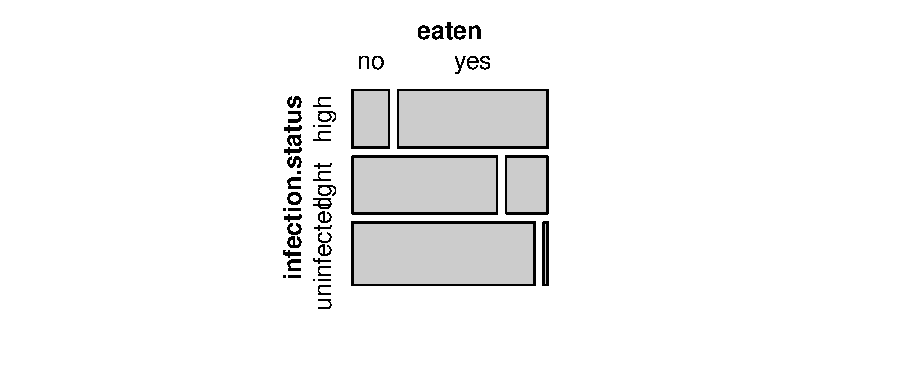
\includegraphics{figures/fig-mosaic1} 

\end{kframe}}
\end{knitrout}

\authNote{NH: this is pretty boring, but I couldn't get "sector" to display
as the second variable without major headaches}
\authNote{NH: can we standardize on either the use of mosaic (from vcd, which
has a confusing name given our package) or mosaicplot?}
\Caution{The \function{mosaic()} function has nothing to do with 
the \pkg{mosaic} package, they just happen to share the same name.}%



Alternatively, we can send \function{mosaic()} the output of \function{xtabs()}:
\begin{knitrout}
\definecolor{shadecolor}{rgb}{.97, .97, .97}{\color{fgcolor}\begin{kframe}
\begin{flushleft}
\ttfamily\noindent
\hlfunctioncall{mosaic}\hlkeyword{(}\hlfunctioncall{xtabs}\hlkeyword{(}\hlkeyword{\urltilda{}}\hlsymbol{sex}{\ }\hlkeyword{+}{\ }\hlsymbol{union}\hlkeyword{,}{\ }\hlsymbol{CPS}\hlkeyword{)}\hlkeyword{)}{\ }{\ }\hlcomment{\usebox{\hlnormalsizeboxhash}{\ }non-whites{\ }are{\ }more{\ }likely{\ }to{\ }be{\ }unionized}\mbox{}
\normalfont
\end{flushleft}
\begin{verbatim}
    union Not Union
sex                
F         217    28
M         221    68
\end{verbatim}
\end{kframe}}
\end{knitrout}

\FoodForThought{Neither \function{mosaic()} nor the similar \function{mosaicplot()}
are as clever as one could hope.  In particular, without some extra customization,
both tend to look bad if the levels of the variables have long names.
\function{mosaic()} plots also always stay square.}


Or we can send our own hand-made table (although the output isn't quite as nice without some
extra effort we won't discuss just now):
\begin{knitrout}
\definecolor{shadecolor}{rgb}{.97, .97, .97}{\color{fgcolor}\begin{kframe}
\begin{flushleft}
\ttfamily\noindent
\hlfunctioncall{mosaic}\hlkeyword{(}\hlsymbol{mycrosstable}\hlkeyword{)}\mbox{}
\normalfont
\end{flushleft}
\end{kframe}}
\end{knitrout}




\begin{problem}
The \dfn{Utilities2} data set in the \verb!mosaic! package contains a number of variables
about the utilities bills at a residence in Minnesota over a number of years.
Since the number of days in a billing cycle varies from month to month, variables 
like \vn{gasbillpday} (\dfn{elecbillpday}, etc.) contain the gas bill (electric bill, etc.) 
divided by the number of days in the billing cycle.
\begin{enumerate}
\item
Make a scatter plot of \dfn{gasbillpday} vs. \dfn{monthsSinceY2K} using the command
\begin{knitrout}
\definecolor{shadecolor}{rgb}{.97, .97, .97}{\color{fgcolor}\begin{kframe}
\begin{flushleft}
\ttfamily\noindent
\hlfunctioncall{xyplot}\hlkeyword{(}\hlsymbol{gasbillpday}{\ }\hlkeyword{\urltilda{}}{\ }\hlsymbol{monthsSinceY2K}\hlkeyword{,}{\ }\hlargument{data}{\ }\hlargument{=}{\ }\hlsymbol{Utilities2}\hlkeyword{,}{\ }\hlargument{type}{\ }\hlargument{=}{\ }\hlstring{"{}l"{}}\hlkeyword{)}{\ }{\ }\hlcomment{\usebox{\hlnormalsizeboxhash}{\ }the{\ }letter{\ }l}\mbox{}
\normalfont
\end{flushleft}
\end{kframe}}
\end{knitrout}

\item[]
What pattern(s) do you see?
\item
What does \verb!type='l'! do?  Make your plot with and without it.  Which is easier to read
in this situation?
\item
What happens if we replace 
\verb!type='l'! with 
\verb!type='b'!?
\item
Make a scatter plot of \vn{gasbillpday} by \vn{month}.   
What do you notice?

\item
Make side-by-side boxplots of \vn{gasbillpday} by \vn{month} using the \dfn{Utilities2}
data frame.   
What do you notice?

Your first try probably won't give you what you expect.  The reason is that month is coded
using numbers, so \R\ treats it as numerical data.  We want to treat it as categorical data.
To do this in \R\, use \verb!factor(month)! in place of \dfn{month}.  
\R\ calls categorical data a \term{factor}.

\item
Make any other plot you like using this data.  Include both a copy of your plot and a 
discussion of what you can learn from it.
\end{enumerate}
\end{problem}

\begin{problem}
The table below is from a study of nighttime lighting in infancy and 
eyesight (later in life).  
% latex table generated in R 2.12.1 by xtable 1.5-6 package
% Fri Feb  4 15:46:48 2011
\begin{center}
\begin{tabular}{rrrr}
  \hline
 & no myopia & myopia & high myopia \\ 
  \hline
darkness & 155 & 15 & 2 \\ 
  nightlight & 153 & 72 & 7 \\ 
  full light & 34 & 36 & 3 \\ 
   \hline
\end{tabular}
\end{center}

\begin{enumerate}
%\item
%Do you think this was an experiment or an observational study?  Why?
\item
Recreate the table in \Rstudio.  %Copy and paste the results into your Word document.
\item
What percent of the subjects slept with a nightlight as infants?

There are several ways to do this.  You could use \R\ as a calculator to do the arithmetic.
You can save some typing if you use the function \verb!prop.table()!.  See
\verb!?prop.table! for documentation.
If you just want row and column totals added to the table, see \verb!mar_table()!
in the \verb!vcd! package.
\item
Make a mosaic plot for this data.  What does this plot reveal?
\end{enumerate}
\end{problem}

Barcharts can also be used to display two-way tables.  First we convert
the cross-table to a data frame.
Then we can use this data frame for plotting.

\begin{knitrout}
\definecolor{shadecolor}{rgb}{.97, .97, .97}{\color{fgcolor}\begin{kframe}
\begin{flushleft}
\ttfamily\noindent
\hlsymbol{cps}{\ }\hlassignement{\usebox{\hlnormalsizeboxlessthan}-}{\ }\hlfunctioncall{as.data.frame}\hlkeyword{(}\hlfunctioncall{xtabs}\hlkeyword{(}\hlkeyword{\urltilda{}}\hlsymbol{sector}{\ }\hlkeyword{+}{\ }\hlsymbol{race}\hlkeyword{,}{\ }\hlargument{data}{\ }\hlargument{=}{\ }\hlsymbol{CPS}\hlkeyword{)}\hlkeyword{)}\hspace*{\fill}\\
\hlstd{}\hlsymbol{cps}\mbox{}
\normalfont
\end{flushleft}
\begin{verbatim}
     sector race Freq
1  clerical   NW   15
2     const   NW    3
3     manag   NW    6
4     manuf   NW   11
5     other   NW    5
6      prof   NW    7
7     sales   NW    3
8   service   NW   17
9  clerical    W   82
10    const    W   17
11    manag    W   49
12    manuf    W   57
13    other    W   63
14     prof    W   98
15    sales    W   35
16  service    W   66
\end{verbatim}
\end{kframe}}
\end{knitrout}

\begin{knitrout}
\definecolor{shadecolor}{rgb}{.97, .97, .97}{\color{fgcolor}\begin{kframe}
\begin{flushleft}
\ttfamily\noindent
\hlfunctioncall{barchart}\hlkeyword{(}\hlsymbol{Freq}{\ }\hlkeyword{\urltilda{}}{\ }\hlsymbol{sector}\hlkeyword{,}{\ }\hlargument{groups}{\ }\hlargument{=}{\ }\hlsymbol{race}\hlkeyword{,}{\ }\hlargument{data}{\ }\hlargument{=}{\ }\hlsymbol{cps}\hlkeyword{)}\mbox{}
\normalfont
\end{flushleft}
\end{kframe}}
\end{knitrout}


\begin{knitrout}
\definecolor{shadecolor}{rgb}{.97, .97, .97}{\color{fgcolor}\begin{kframe}


\centering{}\includegraphics{figures/fig-barchart3b} 

\end{kframe}}
\end{knitrout}




\vspace{-8mm}
\section{Additional Notes on R Syntax}


\subsection{Text and Quotation Marks}

For the most part, text in \R\ must be enclosed in either single or double quotations.  
It usually doesn't matter which you use, unless you want one or the other type of 
quotation mark \emph{inside} your text.  Then you should use the other type of 
quotation mark to mark the beginning and the end.

\begin{knitrout}
\definecolor{shadecolor}{rgb}{.97, .97, .97}{\color{fgcolor}\begin{kframe}
\begin{flushleft}
\ttfamily\noindent
\hlsymbol{text1}{\ }\hlassignement{\usebox{\hlnormalsizeboxlessthan}-}{\ }\hlstring{"{}Mary{\ }didn\usebox{\hlnormalsizeboxsinglequote}t{\ }come"{}}{\ }{\ }\hlcomment{\usebox{\hlnormalsizeboxhash}{\ }apostrophe{\ }inside{\ }requires{\ }double{\ }quotes{\ }around{\ }text}\hspace*{\fill}\\
\hlstd{}\hlsymbol{text2}{\ }\hlassignement{\usebox{\hlnormalsizeboxlessthan}-}{\ }\hlstring{"{}Do{\ }you{\ }use{\ }\usebox{\hlnormalsizeboxbackslash}"{}scare{\ }quotes\usebox{\hlnormalsizeboxbackslash}"{}?"{}}{\ }{\ }\hlcomment{\usebox{\hlnormalsizeboxhash}{\ }this{\ }time{\ }we{\ }flip{\ }things{\ }around}\mbox{}
\normalfont
\end{flushleft}
\end{kframe}}
\end{knitrout}


If you omit quotes, you will often see error messages telling you that \R\ can't find 
an object because \R\
will look for a function, data set or other object with that name instead of treating
your text as text.
\begin{knitrout}
\definecolor{shadecolor}{rgb}{.97, .97, .97}{\color{fgcolor}\begin{kframe}
\begin{flushleft}
\ttfamily\noindent
\hlsymbol{text3}{\ }\hlassignement{\usebox{\hlnormalsizeboxlessthan}-}{\ }\hlsymbol{blah}\mbox{}
\normalfont
\end{flushleft}
\begin{verbatim}
Error: object 'blah' not found
\end{verbatim}
\end{kframe}}
\end{knitrout}


\subsection{Functions}

Functions in \R\ use the following syntax:

\begin{knitrout}
\definecolor{shadecolor}{rgb}{.97, .97, .97}{\color{fgcolor}\begin{kframe}
\begin{flushleft}
\ttfamily\noindent
\hlfunctioncall{functionname}\hlkeyword{(}\hlsymbol{argument1}\hlkeyword{,}{\ }\hlsymbol{argument2}\hlkeyword{,}{\ }\hlsymbol{...}\hlkeyword{)}\mbox{}
\normalfont
\end{flushleft}
\end{kframe}}
\end{knitrout}

\vspace{-5mm}
\begin{itemize}
\item The arguments are \underline{always} \emph{surrounded by (round) parentheses} and 
\emph{separated by commas}.
\begin{itemize}
\item
Some functions (like \verb!col.whitebg()!) 
have no arguments, but you still need the parentheses.
\end{itemize}
\item
Most arguments have names, but you don't need to use the names \emph{if you 
give the arguments in the correct order}.  

If you use names, you can give the arguments out of order.  
The following do the same thing,
%\end{itemize}

\begin{knitrout}
\definecolor{shadecolor}{rgb}{.97, .97, .97}{\color{fgcolor}\begin{kframe}
\begin{flushleft}
\ttfamily\noindent
\hlfunctioncall{xyplot}\hlkeyword{(}\hlsymbol{Sepal.Length}{\ }\hlkeyword{\urltilda{}}{\ }\hlsymbol{Sepal.Width}\hlkeyword{,}{\ }\hlargument{data}{\ }\hlargument{=}{\ }\hlsymbol{iris}\hlkeyword{,}{\ }\hlargument{groups}{\ }\hlargument{=}{\ }\hlsymbol{Species}\hlkeyword{)}\hspace*{\fill}\\
\hlstd{}\hlfunctioncall{xyplot}\hlkeyword{(}\hlsymbol{Sepal.Length}{\ }\hlkeyword{\urltilda{}}{\ }\hlsymbol{Sepal.Width}\hlkeyword{,}{\ }\hlsymbol{iris}\hlkeyword{,}{\ }\hlargument{groups}{\ }\hlargument{=}{\ }\hlsymbol{Species}\hlkeyword{)}\hspace*{\fill}\\
\hlstd{}\hlfunctioncall{xyplot}\hlkeyword{(}\hlsymbol{Sepal.Length}{\ }\hlkeyword{\urltilda{}}{\ }\hlsymbol{Sepal.Width}\hlkeyword{,}{\ }\hlargument{groups}{\ }\hlargument{=}{\ }\hlsymbol{Species}\hlkeyword{,}{\ }\hlsymbol{iris}\hlkeyword{)}\mbox{}
\normalfont
\end{flushleft}
\end{kframe}}
\end{knitrout}

%\begin{itemize}
%\item[]
But these do not work
%\end{itemize}

\begin{knitrout}
\definecolor{shadecolor}{rgb}{.97, .97, .97}{\color{fgcolor}\begin{kframe}
\begin{flushleft}
\ttfamily\noindent
\hlfunctioncall{xyplot}\hlkeyword{(}\hlsymbol{Sepal.Length}{\ }\hlkeyword{\urltilda{}}{\ }\hlsymbol{Sepal.Width}\hlkeyword{,}{\ }\hlsymbol{Species}\hlkeyword{,}{\ }\hlsymbol{iris}\hlkeyword{)}\hspace*{\fill}\\
\hlstd{}\hlfunctioncall{xyplot}\hlkeyword{(}\hlsymbol{Sepal.Length}{\ }\hlkeyword{\urltilda{}}{\ }\hlsymbol{Sepal.Width}\hlkeyword{,}{\ }\hlsymbol{iris}\hlkeyword{,}{\ }\hlsymbol{Species}\hlkeyword{)}\mbox{}
\normalfont
\end{flushleft}
\end{kframe}}
\end{knitrout}

%\begin{itemize}
%\item[]
The first fails because the second argument is \verb!data!, so \verb!iris!
needs to be in the second position if it is not named.
The second fails because \verb!groups! is not the third argument.
(There are many other arguments between \verb!data! and \verb!groups! .)
The documentation for functions shows the correct order of arguments.
\item
Typically, we will not use names for the first argument or two (these tend to be 
very important arguments that have to be there) but will use names for the rest (these 
are often optional arguments that can be present or not, depending on whether we want 
the default behavior or something special).
\end{itemize}

\section{Installing R}

\subsection{RStudio in the cloud}
Our primary version of \R\ will be the online version of \Rstudio.  
You should have an \Rstudio\ account at \url{http://beta.rstudio.org/} 
using your Gmail address.
\Rstudio\ is a brand new (and quite nice) interface to \R\ that runs in a web browser.
This has the advantage that you don't have to install or configure anything.  Just login
and you are good to go.  Futhermore, \Rstudio\ will ``remember'' what you were doing so that
each time you login (even on a different machine) you can pick up right where you left off.
This is ``\R\ in the cloud" and works a bit like GoogleDocs for \R.

If you find bugs or have suggestions for \Rstudio, let us know.  It is in rapid development
at the moment, and we can pass along your feedback to the developers.  

This should be all you need for this course.  But if you prefer to have a
stand-alone version (because you study somewhere without an internet
connection, or have data that can't be loaded into the cloud, for example), read on.


\subsection{RStudio on Your Desktop/Laptop}
There is also a stand-alone version of the \Rstudio\ environment that you can install on
your desktop or laptop machine.  
This can be downloaded from \url{http://www.rstudio.org/}.  This assumes that you 
have a version of R installed on your computer (see below for instructions to download
this from CRAN).


\subsection{Getting R from CRAN}
\label{sec:CRAN}

CRAN is the Comprehensive \R\ Archive Network (\url{http://cran.r-project.org/}).  
You can download free versions of \R\ for PC, Mac, and Linux from CRAN.  (If you use
the \Rstudio\ stand-alone version, you also need to install \R\ this way first.)
All the instructions for downloading and installing are on CRAN.  Just 
follow the appropriate instructions for your platform.

\subsection{RStudio in the cloud on your own server}

At present, we are using a beta version of \RStudio\ running on their servers.  
It is also possible to install this on servers at your institution.  This will
almost certainly require a discussion with your administrators, but may be worthwhile
to facilitate student use in this manner.

\authNoted{NH: Are you both comfortable with this?}


\newpage

\section{\R\ Examples}
\vspace{-3mm}
The commands below are illustrated with the data sets \verb!iris! and 
\verb!CPS!.  To apply these in other situations, you will need to 
substitute the name of your data frame and the variables in it.

\vspace{-3mm}
\begin{center}
\begin{longtable}{p{2.45in}p{3.30in}}
\verb!answer <- 42! & Store the value 42 in a variable named \verb!answer!.
\\[3mm]
%\verb!sl <- iris$Sepal.Length! & Store the \verb!Sepal.Length! variable from the 
%\verb!iris! data frame into a variable called \verb!sl! (to save typing, for example).
%\\[3mm]
\verb!log(123); log10(123); sqrt(123)! & Take natural logarithm, base 10 logarithm, or square 
root of 123.
\\[3mm]
\verb!x <- c(1,2,3)! & Make a variable containing values 1, 2, and 3 (in that order).
\\[3mm]
\verb!data(iris)! & (Re)load the data set \verb!iris!.
\\[3mm]
%\verb!findData(2)! & Find \verb!abd! data in chapter 2.
%\\[3mm]
\verb!summary(iris$Sepal.Length)! & 
Summarize the distribution of the \verb!Sepal.Length! variable in the \verb!iris! data
frame.
\\[3mm]
\verb!summary(iris)! & 
Summarize each variable in the \verb!iris! data frame.
\\[3mm]
\verb!str(iris)! & A different way to summarize the \verb!iris! data frame.
\\[3mm]
\verb!head(iris)! & First few rows of the data frame \verb!iris!.
\\[3mm]
\verb!require(Hmisc)!

\verb!require(abd)!

\ 
& Load packages.  
(This can also be done by checking boxes in the \tab{Packages} tab.)
\\[3mm]
\multicolumn{2}{l}{
\texttt{summary(Sepal.Length\~{}Species,data=iris,fun=favstats) } 
}
\\[1mm]
& 
Compute favorite statistics of \verb!Sepal.Length! for each \verb!Species!.
[requires \verb!Hmisc!]
\\[3mm]
%\verb!cut(x,breaks,right=TRUE)! & Divide up the range of \verb!x! into 
%	intervals and code the values in \verb!x! according to which interval 
%	they fall into. 
%\\[3mm]
\multicolumn{2}{l}{\texttt{histogram(\~{}Sepal.Length|Species, iris)}}
\\[1mm]
& 
Histogram of \verb!Sepal.Length! conditioned on \verb!Species!.
\\[3mm]
\verb!bwplot(Sepal.Length~Species, iris)! & 
Boxplot of \verb!Sepal.Length! conditioned on \verb!Species!.
\\[3mm]
\multicolumn{2}{l}{\texttt{xyplot(Sepal.Length\~{}Sepal.Width|Species, iris)}} 
\\[1mm]
& 
Scatterplot of \verb!Sepal.Length! by \verb!Sepal.Width! 
with separate panels for each  \verb!Species!.
\\[3mm]
\verb!xtabs(~sector, CPS)! & Frequency table of the variable \verb!sector!.
\\[3mm]
\multicolumn{2}{l}{\texttt{barchart(xtabs(\~{}sector, CPS))}}
\\[1mm]
& Make a barchart from the table.
\\[3mm]
\multicolumn{2}{l}{\texttt{xtabs(\~{}sector + race, CPS)}}
\\[1mm]
& Cross tabulation of \verb!sector!  and \verb!race!.
\\[3mm]
\multicolumn{2}{l}{
\texttt{mosaic(\~{}sector + race, CPS)} }
\\[1mm]
& Make a mosaic plot.
\\[3mm]
\multicolumn{2}{l}{
\texttt{xtData <- as.data.frame( xtabs(\~{}sector + race, Trematodes) )}}
\\[1mm]
  & Save cross table information as \verb!xtData!. 
\\[3mm]
\multicolumn{2}{l}{
\texttt{barchart(Freq\~{}sector, data=xtData, groups=race)}
}
\\[1mm]
& Use \verb!xtData! to make a segmented bar chart.
\\[3mm]
\verb!sum(x)!; 
\verb!mean(x)!; 
\verb!median(x)!;

\verb!var(x)!; 
\verb!sd(x)!; 
\verb!quantile(x)!
& Sum, mean, 
median,
variance,
standard deviation,
quantiles of \verb!x!.
\\
\end{longtable}
%\rule{4in}{1pt}
\end{center}

\vspace*{-.5in}
\section{Exercises}

%For these problems, create a single Word document containing all of your work.

\shipoutProblems










\chapter{Getting Interactive with \texttt{manipulate}}

One very attractive feature of \RStudio\ is the \verb!manipulate()! function, which
can allow the creation of a set of controls (such as \verb!slider()!, \verb!picker()!
or \verb!checkbox()!) that can be used to dynamically change values within the 
expression.  When a value is changed using these controls, the expression is automatically
re-executed and redrawn.  This can be used to quickly prototype a number of activities and
demos as part of a statistics lecture.

\section{Simple Things}

\subsection{Sliders}

\authNote{need to remove \emph{if(require)}}

\begin{knitrout}
\definecolor{shadecolor}{rgb}{.97, .97, .97}{\color{fgcolor}\begin{kframe}
\begin{flushleft}
\ttfamily\noindent
\hlkeyword{if}{\ }\hlkeyword{(}\hlfunctioncall{require}\hlkeyword{(}\hlsymbol{manipulate}\hlkeyword{)}\hlkeyword{)}{\ }\hlkeyword{\usebox{\hlnormalsizeboxopenbrace}}\hspace*{\fill}\\
\hlstd{}{\ }{\ }{\ }{\ }\hlfunctioncall{manipulate}\hlkeyword{(}\hlfunctioncall{histogram}\hlkeyword{(}\hlkeyword{\urltilda{}}\hlsymbol{eruptions}\hlkeyword{,}{\ }\hlargument{data}{\ }\hlargument{=}{\ }\hlsymbol{faithful}\hlkeyword{,}{\ }\hlargument{n}{\ }\hlargument{=}{\ }\hlsymbol{n}\hlkeyword{)}\hlkeyword{,}{\ }\hlargument{n}{\ }\hlargument{=}{\ }\hlfunctioncall{slider}\hlkeyword{(}\hlnumber{5}\hlkeyword{,}\hspace*{\fill}\\
\hlstd{}{\ }{\ }{\ }{\ }{\ }{\ }{\ }{\ }\hlnumber{40}\hlkeyword{)}\hlkeyword{)}\hspace*{\fill}\\
\hlstd{}\hlkeyword{\usebox{\hlnormalsizeboxclosebrace}}\mbox{}
\normalfont
\end{flushleft}
\end{kframe}}
\end{knitrout}

This generates a plot along with a slider ranging from 5 bins to 40.

\begin{center}
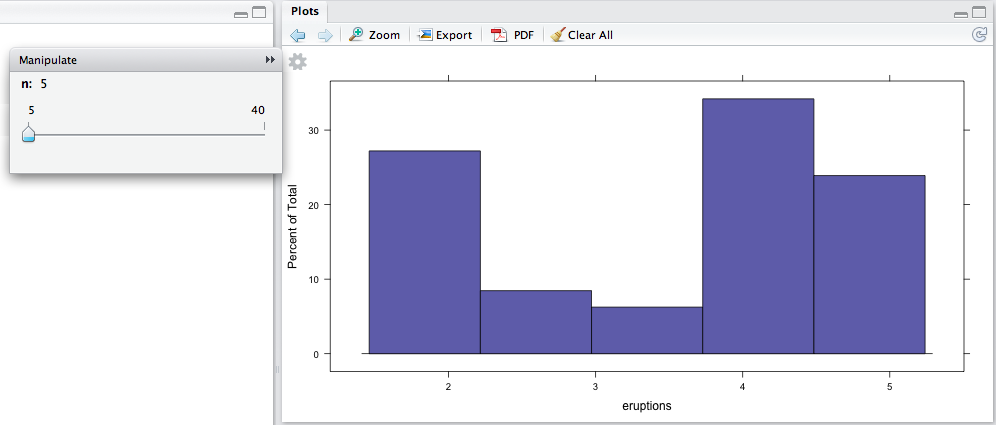
\includegraphics[width=3.8in]{images/manip-hist1.png}
\end{center}

When the slider is changed, we see a clearer view of the eruptions of Old Faithful.

\centerline{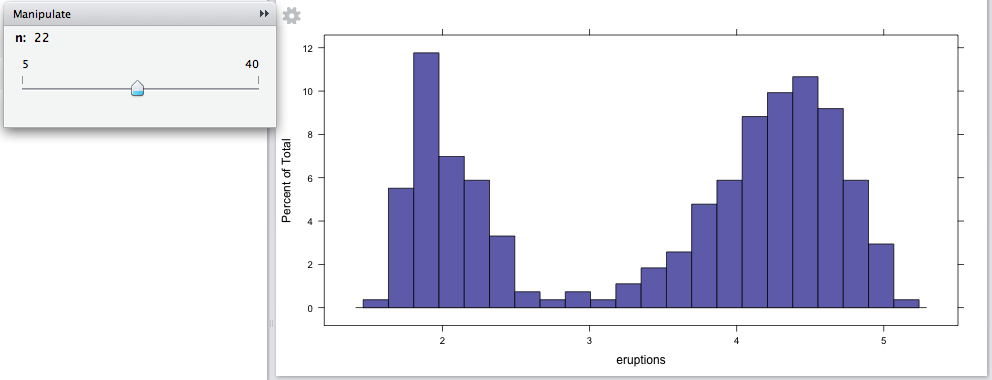
\includegraphics[width=3.8in]{images/manip-hist2.png}}



\subsection{Check Boxes}

\begin{knitrout}
\definecolor{shadecolor}{rgb}{.97, .97, .97}{\color{fgcolor}\begin{kframe}
\begin{flushleft}
\ttfamily\noindent
\hlkeyword{if}{\ }\hlkeyword{(}\hlfunctioncall{require}\hlkeyword{(}\hlsymbol{manipulate}\hlkeyword{)}\hlkeyword{)}{\ }\hlkeyword{\usebox{\hlnormalsizeboxopenbrace}}\hspace*{\fill}\\
\hlstd{}{\ }{\ }{\ }{\ }\hlfunctioncall{manipulate}\hlkeyword{(}\hlfunctioncall{xhistogram}\hlkeyword{(}\hlkeyword{\urltilda{}}\hlsymbol{age}\hlkeyword{,}{\ }\hlargument{data}{\ }\hlargument{=}{\ }\hlsymbol{HELP}\hlkeyword{,}{\ }\hlargument{n}{\ }\hlargument{=}{\ }\hlsymbol{n}\hlkeyword{,}{\ }\hlargument{density}{\ }\hlargument{=}{\ }\hlsymbol{density}\hlkeyword{)}\hlkeyword{,}{\ }\hlargument{n}{\ }\hlargument{=}{\ }\hlfunctioncall{slider}\hlkeyword{(}\hlnumber{5}\hlkeyword{,}\hspace*{\fill}\\
\hlstd{}{\ }{\ }{\ }{\ }{\ }{\ }{\ }{\ }\hlnumber{40}\hlkeyword{)}\hlkeyword{,}{\ }\hlargument{density}{\ }\hlargument{=}{\ }\hlfunctioncall{checkbox}\hlkeyword{(}\hlkeyword{)}\hlkeyword{)}\hspace*{\fill}\\
\hlstd{}\hlkeyword{\usebox{\hlnormalsizeboxclosebrace}}\mbox{}
\normalfont
\end{flushleft}
\begin{verbatim}
Loading required package: manipulate
\end{verbatim}
\begin{verbatim}
Warning message: there is no package called 'manipulate'
\end{verbatim}
\end{kframe}}
\end{knitrout}


\centerline{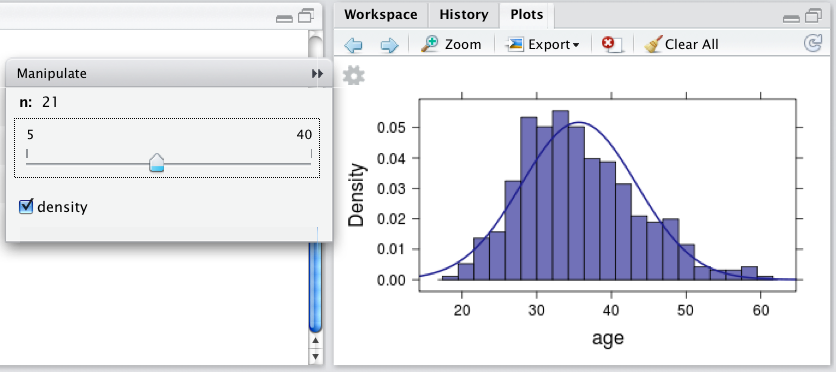
\includegraphics[width=3.8in]{images/manipulate-checkbox}}

\subsection{Drop-down Menus}

\begin{knitrout}
\definecolor{shadecolor}{rgb}{.97, .97, .97}{\color{fgcolor}\begin{kframe}
\begin{flushleft}
\ttfamily\noindent
\hlkeyword{if}{\ }\hlkeyword{(}\hlfunctioncall{require}\hlkeyword{(}\hlsymbol{manipulate}\hlkeyword{)}\hlkeyword{)}{\ }\hlkeyword{\usebox{\hlnormalsizeboxopenbrace}}\hspace*{\fill}\\
\hlstd{}{\ }{\ }{\ }{\ }\hlfunctioncall{manipulate}\hlkeyword{(}\hlfunctioncall{xhistogram}\hlkeyword{(}\hlkeyword{\urltilda{}}\hlsymbol{age}\hlkeyword{,}{\ }\hlargument{data}{\ }\hlargument{=}{\ }\hlsymbol{HELP}\hlkeyword{,}{\ }\hlargument{n}{\ }\hlargument{=}{\ }\hlsymbol{n}\hlkeyword{,}{\ }\hlargument{fit}{\ }\hlargument{=}{\ }\hlsymbol{distribution}\hlkeyword{,}{\ }\hlargument{dlwd}{\ }\hlargument{=}{\ }\hlnumber{4}\hlkeyword{)}\hlkeyword{,}\hspace*{\fill}\\
\hlstd{}{\ }{\ }{\ }{\ }{\ }{\ }{\ }{\ }\hlargument{n}{\ }\hlargument{=}{\ }\hlfunctioncall{slider}\hlkeyword{(}\hlnumber{5}\hlkeyword{,}{\ }\hlnumber{40}\hlkeyword{)}\hlkeyword{,}{\ }\hlargument{distribution}{\ }\hlargument{=}{\ }\hlfunctioncall{picker}\hlkeyword{(}\hlstring{"{}normal"{}}\hlkeyword{,}{\ }\hlstring{"{}gamma"{}}\hlkeyword{,}{\ }\hlstring{"{}exponential"{}}\hlkeyword{,}\hspace*{\fill}\\
\hlstd{}{\ }{\ }{\ }{\ }{\ }{\ }{\ }{\ }{\ }{\ }{\ }{\ }\hlstring{"{}lognormal"{}}\hlkeyword{,}{\ }\hlargument{label}{\ }\hlargument{=}{\ }\hlstring{"{}distribution"{}}\hlkeyword{)}\hlkeyword{)}\hspace*{\fill}\\
\hlstd{}\hlkeyword{\usebox{\hlnormalsizeboxclosebrace}}\mbox{}
\normalfont
\end{flushleft}
\begin{verbatim}
Loading required package: manipulate
\end{verbatim}
\begin{verbatim}
Warning message: there is no package called 'manipulate'
\end{verbatim}
\end{kframe}}
\end{knitrout}


\centerline{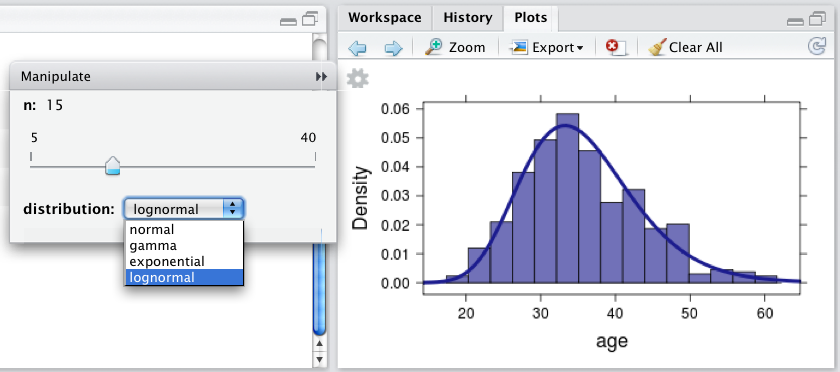
\includegraphics[width=3.8in]{images/manipulate-picker}}

\subsection{Visualizing Normal Distributions}
\begin{knitrout}
\definecolor{shadecolor}{rgb}{.97, .97, .97}{\color{fgcolor}\begin{kframe}
\begin{flushleft}
\ttfamily\noindent
\hlkeyword{if}{\ }\hlkeyword{(}\hlfunctioncall{require}\hlkeyword{(}\hlsymbol{manipulate}\hlkeyword{)}\hlkeyword{)}{\ }\hlkeyword{\usebox{\hlnormalsizeboxopenbrace}}\hspace*{\fill}\\
\hlstd{}{\ }{\ }{\ }{\ }\hlfunctioncall{manipulate}\hlkeyword{(}\hlfunctioncall{xpnorm}\hlkeyword{(}\hlsymbol{x}\hlkeyword{,}{\ }\hlnumber{500}\hlkeyword{,}{\ }\hlnumber{100}\hlkeyword{)}\hlkeyword{,}{\ }\hlargument{x}{\ }\hlargument{=}{\ }\hlfunctioncall{slider}\hlkeyword{(}\hlnumber{200}\hlkeyword{,}{\ }\hlnumber{800}\hlkeyword{)}\hlkeyword{)}\hspace*{\fill}\\
\hlstd{}\hlkeyword{\usebox{\hlnormalsizeboxclosebrace}}\mbox{}
\normalfont
\end{flushleft}
\begin{verbatim}
Loading required package: manipulate
\end{verbatim}
\begin{verbatim}
Warning message: there is no package called 'manipulate'
\end{verbatim}
\end{kframe}}
\end{knitrout}

\centerline{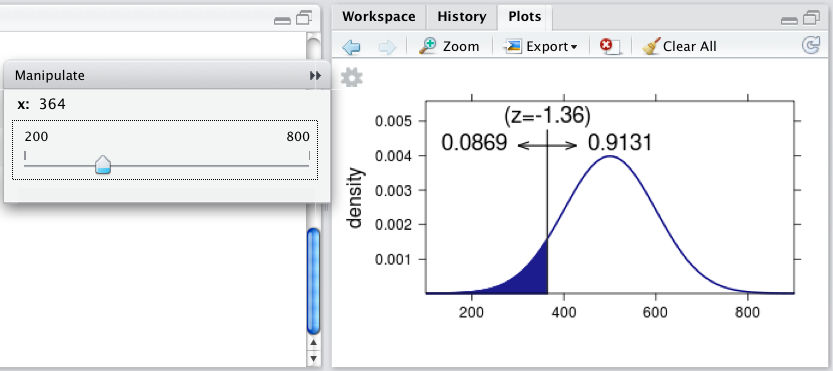
\includegraphics[width=3.8in]{images/manipulate-xpnorm}}


\begin{problem}
The following code makes a scatterplot with separate symbols for each sex.
\begin{knitrout}
\definecolor{shadecolor}{rgb}{.97, .97, .97}{\color{fgcolor}\begin{kframe}
\begin{flushleft}
\ttfamily\noindent
\hlfunctioncall{xyplot}\hlkeyword{(}\hlsymbol{cesd}{\ }\hlkeyword{\urltilda{}}{\ }\hlsymbol{age}\hlkeyword{,}{\ }\hlargument{data}{\ }\hlargument{=}{\ }\hlsymbol{HELP}\hlkeyword{,}{\ }\hlargument{groups}{\ }\hlargument{=}{\ }\hlsymbol{sex}\hlkeyword{)}\mbox{}
\normalfont
\end{flushleft}
\end{kframe}}
\end{knitrout}

Build a \pkg{manipulate} example that allows you to turn the grouping on and off with a 
checkbox.
\end{problem}

\begin{problem}
Build a \pkg{manipulate} example that uses a picker to select from a number of 
variables to make a plot for.  Here's an example with a histogram:

\medskip
\centerline{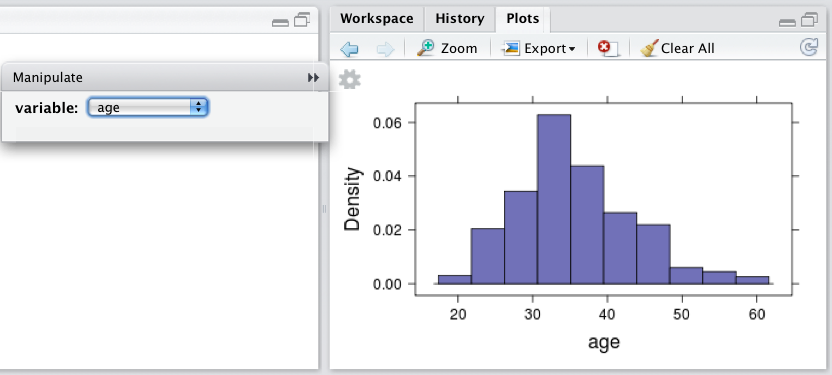
\includegraphics[width=3.8in]{images/manipulate-multihist}}
\end{problem}

\begin{problem}
Design your own  interactive demonstration idea and implement it using 
\RStudio\ \pkg{manipulate} tools.
\end{problem}

\section*{Exercises}
\shipoutProblems



\chapter{Multivariate Statistics -- Early?} 
\label{chap:multivariate-early}







If you are of a certain age, you may remember the 1960s television show {\em
  Lost in Space}.  One of the characters, the Robot, was often
assigned guard duty.  Robot would march back and forth, just like a
soldier on guard duty.

But why?  Soldiers are ordered to march back and forth so that they
won't fall asleep; walking forces them to maintain a certain attention
to their duty.  Robot has no such need; his sensors and circuits can reliably
detect intruders without the marching.  Of course, the television
viewers wouldn't know this about robots.  Using the robot in the
manner of a soldier was a way to introduce new technology to people
with old mind-sets.

Now fast forward from the television of the 1960s to the classroom of
the 21st century.  Students have computers.  They use statistical
software packages to do calculations.  But what calculations are they
doing?  Sample means, sample proportions, differences between means.

This is Robot walking back and forth.  A way to use new technology with
old mind-sets.  But it's the professors, not the students, with the
old mind-sets.  The students are open to new things.  They don't need
to know that, once upon a time, it was a feat to get a machine to add
up a column of numbers.

We professors were educated at a time when the tools for inverting a
matrix were paper and pencil, when doing least squares problem involved
a strange thing called a ``pseudo-inverse'' that you might learn in
your fourth or fifth semester of university-level mathematics.  But, now, least squares
problems are no more difficult or time consuming to the human than
square roots or addition.  We just have to learn to use the tools in
the right way.  

Or, rather, we have to show our students what are the
basic operations that are important for statistical reasoning in an
age of modern computation.  Not marching back and forth, like robot
soldiers, computing sums of columns of numbers, but thinking about how to model the
potentially rich interplay among multiple variables.

The standard approach to introductory statistics is based on a few
simple operations: adding, squaring, and square-rooting to finding means 
and standard deviations; 
counting to find proportions and medians/quantiles.  These operations are
(supposed to be) familiar to students from high-school mathematics.

Here we'll examine the consequences of adding in a new basic operation
that is not in the traditional high-school curriculum, but which is
actually quite consistent with the ``Common Core'' curriculum being
introduced by many U.S. states.\cite{common-core-2010}


The operation is fitting multivariate linear models.  Modern software
makes it no more arduous than finding a mean or standard deviation.
Our emphasis here will be on how to introduce the conceptual
foundations --- using just high-school math and simple extensions
largely specified already in the ``Common Core'' --- that make the concept
of modeling accessible.

There are three important pedagogical advantages to using multivariate linear models
as a foundation for statistics:
\begin{enumerate}
  \item It provides a logically coherent framework that unifies many
    of the disparate techniques found in introductory statistics books.
  \item It allows the very important ideas of confounding and
    covariates to be introduced in an integrated way, showing students
    not only the perils of confounding, but what to do about it (and
    when you can't do anything).
  \item It allows the examples used in classes to be drawn from a
    richer set of situations, and provides scope for students to
    express their creativity and insight.  This can increase student
    motivation.
\end{enumerate}
Of course, it's also important that modern statistical work is already
and increasingly shaped by multivariate methods.  For an example of
how over the last few decades statistical methods used in the
literature have shifted away from the curriculum of the traditional,
non-multivariate introductory course, see the review of statistics
practices in the \emph{New England Journal of Medicine}. \cite{switzer-horton-2005}

\section{The Mathematical Foundations}

A standard part of the high-school curriculum is the equation of a
straight line: $y = m x + b$.  Many students will recognize that $m$
is a slope and $b$ is the $y$-intercept.  

It's helpful to move them a bit beyond this:
\begin{itemize}
\item Emphasize the ``function'' concept.  A function, of course, is a
  relationship between an input and an output.  Generalize this, so
  that students are comfortable with using names other than $x$ as the
  input and
  $y$ as the output.  For example, 
  $$\mbox{height} = f( \mbox{age} ) = 3\ \mbox{age} + 20$$.
  
\item Introduce the idea of functions of non-numeric variables, for example:
$$\mbox{height} = g( \mbox{sex} ) = \left\{ \begin{array}{ll}
      67 & \mbox{for sex $=$ female}\\
      71 & \mbox{for sex $=$ male}\\
      \end{array}\right.$$
   
\item Generalize the idea of a function to include having more than
  one input, for instance

$$\mbox{height} = h( \mbox{age}, \mbox{sex} ) = -2\ \mbox{age} + 
      \left\{ \begin{array}{ll}
      67 & \mbox{for sex $=$ female}\\
      71 & \mbox{for sex $=$ male}\\
      \end{array}\right.$$

\item  De-program your students from thinking that there is one, and
  only one, correct formula for a relationship.  Introduce the idea of a function as a
  description of a relationship and that there can be different descriptions of the same
  relationship, all of which can be right in some ways.  Different
  descriptions can include some details and exclude others. Such
  descriptions are called ``models.''  The above models
  $f(\mbox{age})$, and $g(\mbox{sex})$ and $h(\mbox{age}, \mbox{sex})$
  give different outputs for the same inputs.  For example, for a male
  of age 10, according to the models, the height is variously $f(10) =
  50$ or $g(\mbox{male}) = 71$ or $h(10, \mbox{male}) = 51$.
  
\item  Many useful models don't give exactly the right output for
  every case.  Not every 10-year old male has the same height.  The
  difference between what a model says, and what the value is for an
  actual case, will not in general be zero.  The ``residual'' is the difference between
  the actual value for a given 10-year old male, say Ralph, and what
  a given model says about 10-year old males in general.  The
  residuals give important information about how good a model is.
   
\end{itemize}


\section{The Language of Models}
\label{sec:formula}

There is a language for defining models that is different from
writing down an algebraic formula.  

You have already seen some aspects of this notation in graphics
commands, e.g. \verb!height ~ sex!.  You can read this in any of several
ways:
\begin{itemize}
  \item Break down \VN{height} by \VN{sex} (as in a boxplot)
  \item \VN{height} versus \VN{sex}
  \item Model \VN{height} as a function of \VN{sex}.  
\end{itemize}
In this section, you'll see more complicated models, involving
multiple variables.  This makes it worthwhile to assign more precise
labels to the different components of the modeling language, which
has just a few components:
\begin{itemize}
  \item The response variable.  This is the output of the model function,
    \VN{height} in the above examples.
  \item The explanatory variables.  These are the inputs to the
    model function: \VN{age} and \VN{sex} in the above examples.
  \item Model terms.  Examples of model terms are explanatory
    variables themselves and a special term called the ``intercept.''
    There are a few others, but we'll deal with them as we come to them.
\end{itemize}
(A more comprehensive introduction is given in Chapters 4 and 5 of \cite{kaplan-2009-book}.)


As an example, consider this simple formula:
$$ z = 7 + 3 x + 4.5 y.$$
The corresponding model description consists of the response variable
$z$, and three model terms: the explanatory variables $x$ and
$y$ and the intercept term.  In the modeling language, it would be written:
\begin{quotation}
\centerline{\model{z}{1 + x + y}}
\end{quotation}
Notice that instead of the $=$ sign, we are using the $\sim$ sign.
Also, notice that the specific coefficients $7$, $3$, and $4.5$ are
missing.  The model description is a kind of skeleton for describing
the shape of the model.  It's like saying: ``We want a straight line
model,'' rather than giving the complete specification of the formula.

The process of finding a specific formula to make a model match the
pattern shown by data is called ``fitting the model to the data.''  

To see how different model specifications correspond to different
``shapes'' of models, consider the history of world-record times in the 100-meter 
free-style swimming race.








\begin{knitrout}
\definecolor{shadecolor}{rgb}{.97, .97, .97}{\color{fgcolor}\begin{kframe}


\centering{}\includegraphics{figures/fig-swim-data-raw21} \includegraphics{figures/fig-swim-data-raw22} 

\end{kframe}}
\end{knitrout}




You can see the steady improvement in records over the decades from
1900 to the present.  Men's times are somewhat faster than women's.

Now to build some models.

\subsection{\model{\VN{Time}}{\VN{1} + \VN{Year}}}

The model \model{\VN{time}}{1 + \VN{year}} gives the familiar
straight-line form: the intercept term (written simply as 1) and a term corresponding to the
linear dependence on \VN{year}.





\begin{knitrout}
\definecolor{shadecolor}{rgb}{.97, .97, .97}{\color{fgcolor}\begin{kframe}


\centering{}\includegraphics{figures/fig-swim-data-1b1} \includegraphics{figures/fig-swim-data-1b2} 

\end{kframe}}
\end{knitrout}


This model captures some of the pattern evident in the data: that
swimming times are improving (getting shorter) over the years.  And it
ignores other obvious features, for example the difference between men's
and women's times, or the curvature reflecting that records are not
improving as fast as they did in the early days.


\subsection{\model{\VN{Time}}{\VN{Sex}}}

The model \model{\VN{time}}{\VN{sex}} breaks down the swimming times
according to \VN{sex}:

\begin{knitrout}
\definecolor{shadecolor}{rgb}{.97, .97, .97}{\color{fgcolor}\begin{kframe}


\centering{}\includegraphics{figures/fig-swim-data-21} \includegraphics{figures/fig-swim-data-22} 

\end{kframe}}
\end{knitrout}


This model reflects the typical difference between men's and women's
times.  It's oblivious to the trend that records improve over the
years.  Why?  Because the variable \VN{year} was not included in the model.

\subsection{\model{\VN{Time}}{\VN{Sex}+\VN{Year}}}

The record time evidently depends both on \VN{sex} and \VN{year}, so
it's sensible to include both variables in the model

\begin{knitrout}
\definecolor{shadecolor}{rgb}{.97, .97, .97}{\color{fgcolor}\begin{kframe}


\centering{}\includegraphics{figures/fig-swim-data-31} \includegraphics{figures/fig-swim-data-32} 

\end{kframe}}
\end{knitrout}


\authNote{DTK: Should these graphics be re-written to display as
  continuous forms rather than dots?}

This is a straight-line model with separate lines for the different
sexes. The intercept is different for the different sexes, but the
slope is the same.  
This model is reflects the typical difference between men's and women's
times.  

Students sometimes observe that the function generated by fitting this
model doesn't respect the ``vertical line test'' taught in high-school
algebra.  This is a good time to remind students that this is a
function of \emph{two} variables.  It is indeed a function, and for
any specific value of the inputs \VN{sex} and \VN{year} gives a single value.

\subsection{\model{\VN{Time}}{\VN{Sex}+\VN{Year} + \VN{Sex}:\VN{Year}}}
 
There are two ways that the previous model, \model{\VN{time}}{\VN{sex}+\VN{year}},  misses obvious features in the
data: there is no curvature over the years and the slopes are exactly
the same for men and women.  To construct a model with different
slopes for men and women requires that we add a term that combines
both \VN{sex} and \VN{year}.  Such a term is constructed with the syntax
\VN{sex}:\VN{year} (or, what would amount to the same thing,
\VN{year}:\VN{sex}).  

\begin{knitrout}
\definecolor{shadecolor}{rgb}{.97, .97, .97}{\color{fgcolor}\begin{kframe}


\centering{}\includegraphics{figures/fig-swim-data-41} \includegraphics{figures/fig-swim-data-42} 

\end{kframe}}
\end{knitrout}


In statistics, such a term is called an \emph{interaction term}.  (In
mathematics, it's often called a \emph{bi-linear term}.)  It's the
term that lets you have different slopes for the different sexes.  

The new phrase ``interaction term'' creates a need for a retronym, a way
to refer to those simple, non-interaction terms that we started with,
like \VN{sex} and \VN{year}.  (Common retronyms in everyday life are acoustic guitar, snail-mail, 
World War I, cloth diaper, and whole milk, compound terms that weren't needed
until electric guitars, e-mail, disposable diapers, and skim milk were
introduced, and World War II showed that the ``War to End All Wars''
was mis-named.)

The standard terminology for terms like \VN{sex} and \VN{year} is unfortunate: ``main effect.'' 
It suggests that interaction terms play a lesser role in modeling.  This is a bad
attitude, since sometimes the interaction is exactly what you're
interested in, but the terminology seems enshrined by statistical tradition.

Very often when you are including an interaction term, you want to
include the main effects as well.  There is a convenient shorthand for
this: \model{\VN{time}}{\VN{sex}*\VN{year}}

\subsection{The Intercept Only: \model{\VN{Time}}{\VN{1}}}

It's also possible to have models that have no explanatory variables
whatsoever.  Just the intercept term appears to the right of the
model formula. 

\begin{knitrout}
\definecolor{shadecolor}{rgb}{.97, .97, .97}{\color{fgcolor}\begin{kframe}


\centering{}\includegraphics{figures/fig-swim-data-51} \includegraphics{figures/fig-swim-data-52} 

\end{kframe}}
\end{knitrout}


As you might expect, by leaving out both \VN{sex} and \VN{year} from
the model, it doesn't reflect the role of either variable in any way.
But the model \model{\VN{time}}{1} does get one thing very well: the
typical record time.  

Think of \model{\VN{time}}{1} as saying ``all the cases are the
same.''  In some ways, it's analogous to the model
\model{\VN{time}}{\VN{sex}}.  That model says that ``all men are the
same, and all women are the same.''  So the difference between 
\model{\VN{time}}{1} and \model{\VN{time}}{\VN{sex}} is just like the
difference between a ``grand mean'' and a ``group mean.''

\subsection{Transformation Terms}

You can construct more complicated models by adding in more
explanatory variables. (Improved swimming gear?  Better training?
Refinements in technique?).  You can also add in additional terms with
more structure.  There is a rich variety of ways to do this.

Since many students are familiar (or at least remember vaguely) the
idea of quadratics and polynomials, they might be interested to see
that the modeling language can handle this.  Here are three different
models involving a polynomial dependence on \VN{year}:

\begin{knitrout}
\definecolor{shadecolor}{rgb}{.97, .97, .97}{\color{fgcolor}\begin{kframe}


\centering{}\includegraphics{figures/fig-swim-data-61} \includegraphics{figures/fig-swim-data-62} 

\end{kframe}}
\end{knitrout}


\begin{knitrout}
\definecolor{shadecolor}{rgb}{.97, .97, .97}{\color{fgcolor}\begin{kframe}


\centering{}\includegraphics{figures/fig-swim-data-71} \includegraphics{figures/fig-swim-data-72} 

\end{kframe}}
\end{knitrout}


\begin{knitrout}
\definecolor{shadecolor}{rgb}{.97, .97, .97}{\color{fgcolor}\begin{kframe}


\centering{}\includegraphics{figures/fig-swim-data-81} \includegraphics{figures/fig-swim-data-82} 

\end{kframe}}
\end{knitrout}


Although these models reflect more ``detail'' in the data, namely the
curvature, they do it in a way that ultimately does not make sense in
terms of the ``physics'' of world records.
Notice how the upward facing parabolas eventually produce a pattern
where the record times increase over the years.  

There are other sorts of nonlinear terms that might be more
appropriate for modeling this sort of data.  Exponentials, square
roots, etc., even piecewise linear or bent-line forms are all
possible within the modeling framework.  


\begin{problem}
{\bf DRAFT Outline} for a swim-data modeling problem: construct a post-war
variable and add it in.  Several ways to do this: explore which one's give
models that are most satisfactory to you:
\begin{itemize}
  \item postwar = year $>$ 1945
  \item interaction with postwar and year.
  \item pmax(year - 1945, 0)
\end{itemize}
\end{problem}





\section{Finding Formulas from Data}

Behind the graphical depictions of the models shown in the previous
section is a process for finding specific numerical formulas for the
models.  The software to do this is packaged into the \texttt{lm( )}
operator and is very easy for students and professionals alike.  The
human work, and what students need to learn, is not the mechanics of
fitting models, but the interpretation of them.  A good place to start
is with the interpretation of model coefficients.

To illustrate, consider the actual swimming records data employed in
the previous examples.  This data set is available via the internet,
and can be loaded into R with a command like the following:

\authNote{DTK: Eventually, we have to build into MOSAIC an easy way
  for instructors to specify a web location for their data.  The
  \texttt{ISMdata( )} function already does this in a limited way.}

\begin{knitrout}
\definecolor{shadecolor}{rgb}{.97, .97, .97}{\color{fgcolor}\begin{kframe}
\begin{flushleft}
\ttfamily\noindent
\hlsymbol{swim}{\ }\hlassignement{=}{\ }\hlfunctioncall{read.csv}\hlkeyword{(}\hlstring{"{}http://www.macalester.edu/\urltilda{}kaplan/ISM/datasets/swim100m.csv"{}}\hlkeyword{)}\mbox{}
\normalfont
\end{flushleft}
\end{kframe}}
\end{knitrout}


\authNote{DTK: I couldn't stand the default printing of lm, so I
  changed it. We might want to do this more generally, but it's not
  something we need to worry about here.}



As before, we'll model the world-record \VN{time} as a function of \VN{sex}
and \VN{year}.

Here's the very simplest model: all cases are modeled as being the same.
\begin{knitrout}
\definecolor{shadecolor}{rgb}{.97, .97, .97}{\color{fgcolor}\begin{kframe}
\begin{flushleft}
\ttfamily\noindent
\hlfunctioncall{lm}\hlkeyword{(}\hlsymbol{time}{\ }\hlkeyword{\urltilda{}}{\ }\hlnumber{1}\hlkeyword{,}{\ }\hlargument{data}{\ }\hlargument{=}{\ }\hlsymbol{swim}\hlkeyword{)}\mbox{}
\normalfont
\end{flushleft}
\begin{verbatim}
Coefficients:
(Intercept)  
       59.9  

\end{verbatim}
\end{kframe}}
\end{knitrout}

The fundamental purpose of \texttt{lm( )} is to find the coefficients
that flesh out the skeleton provided by the model description.  For
this simple model, the coefficient works out to be the mean of the
record times:
\begin{knitrout}
\definecolor{shadecolor}{rgb}{.97, .97, .97}{\color{fgcolor}\begin{kframe}
\begin{flushleft}
\ttfamily\noindent
\hlfunctioncall{with}\hlkeyword{(}\hlargument{data}{\ }\hlargument{=}{\ }\hlsymbol{swim}\hlkeyword{,}{\ }\hlfunctioncall{mean}\hlkeyword{(}\hlsymbol{time}\hlkeyword{)}\hlkeyword{)}\mbox{}
\normalfont
\end{flushleft}
\begin{verbatim}
 mean 
59.92 
\end{verbatim}
\end{kframe}}
\end{knitrout}

\authNote{DTK: I'm looking forward to being able to write mean(time, data=swim).}

Models are more interesting that contain actual explanatory
variables.  Here's one using the quantitative variable \VN{year}:
\begin{knitrout}
\definecolor{shadecolor}{rgb}{.97, .97, .97}{\color{fgcolor}\begin{kframe}
\begin{flushleft}
\ttfamily\noindent
\hlfunctioncall{lm}\hlkeyword{(}\hlsymbol{time}{\ }\hlkeyword{\urltilda{}}{\ }\hlsymbol{year}\hlkeyword{,}{\ }\hlargument{data}{\ }\hlargument{=}{\ }\hlsymbol{swim}\hlkeyword{)}\mbox{}
\normalfont
\end{flushleft}
\begin{verbatim}
Coefficients:
(Intercept)         year  
     567.24        -0.26  

\end{verbatim}
\end{kframe}}
\end{knitrout}

The coefficients now are the slope and intercept of the straight-line
relationship: $\mbox{time}  = -0.2599 \mbox{year} + 567.242$.

There's a similar story with categorical variables, like \VN{sex}:
\begin{knitrout}
\definecolor{shadecolor}{rgb}{.97, .97, .97}{\color{fgcolor}\begin{kframe}
\begin{flushleft}
\ttfamily\noindent
\hlfunctioncall{lm}\hlkeyword{(}\hlsymbol{time}{\ }\hlkeyword{\urltilda{}}{\ }\hlsymbol{sex}\hlkeyword{,}{\ }\hlargument{data}{\ }\hlargument{=}{\ }\hlsymbol{swim}\hlkeyword{)}\mbox{}
\normalfont
\end{flushleft}
\begin{verbatim}
Coefficients:
(Intercept)         sexM  
       65.2        -10.5  

\end{verbatim}
\end{kframe}}
\end{knitrout}

Based on the result of the simple all-cases-the-same model
\model{\VN{time}}{1}, you might suspect that the coefficients are the
group means.  That's close to being right.  Here are the group means:
\begin{knitrout}
\definecolor{shadecolor}{rgb}{.97, .97, .97}{\color{fgcolor}\begin{kframe}
\begin{flushleft}
\ttfamily\noindent
\hlfunctioncall{mean}\hlkeyword{(}\hlsymbol{time}{\ }\hlkeyword{\urltilda{}}{\ }\hlsymbol{sex}\hlkeyword{,}{\ }\hlargument{data}{\ }\hlargument{=}{\ }\hlsymbol{swim}\hlkeyword{)}\mbox{}
\normalfont
\end{flushleft}
\begin{verbatim}
  sex     S  N Missing
1   F 65.19 31       0
2   M 54.66 31       0
\end{verbatim}
\end{kframe}}
\end{knitrout}

\InstructorNote{In the MOSAIC package, the syntax of familiar
  operators like \texttt{mean( )}, \texttt{sd( )}, etc. has been
  extended so that the modeling notation can be used to calculate
  group-by-group values.  Our goal is to make is straightforward to
  transition from conventional basic stats to modeling, by getting
  students used to the $\sim$ and \texttt{data=} notation early.  You
  can even do \texttt{mean( time}$ ~ $ \texttt{ 1, data=swim )}. 
  So you can talk about models in a systematic way even if all you want to cover is means,
  proportions, medians, etc.}


The coefficients of the linear model are organized differently than
simple group means.
Notice that there is a \VN{sexM} coefficient, but no similarly named
coefficient for women.  Instead, there is the intercept coefficient.  
This corresponds to the mean \VN{time} of one
of the groups: the reference group.  In this case, the reference group
is women.  

The other coefficient, \VN{sexM} tells the
\emph{difference} between the mean of the reference group and the mean
for the men.  In other words, the coefficients are arranged in
intercept-slope form, but for categorical variables the coefficient
isn't a slope but a finite-difference.  

\InstructorNote{The intercept is so important that the \texttt{lm( )}
  operator includes it by default, even if you don't specify it
  explicitly in the model design.  In those rare cases when you don't
  want an intercept term, use the notation \texttt{-1} as part of the
  model design.}


It's important to keep in mind the intercept-slope/difference format
when interpreting the coefficients from models with multiple
explanatory variables:
\begin{knitrout}
\definecolor{shadecolor}{rgb}{.97, .97, .97}{\color{fgcolor}\begin{kframe}
\begin{flushleft}
\ttfamily\noindent
\hlfunctioncall{lm}\hlkeyword{(}\hlsymbol{time}{\ }\hlkeyword{\urltilda{}}{\ }\hlsymbol{sex}{\ }\hlkeyword{+}{\ }\hlsymbol{year}\hlkeyword{,}{\ }\hlargument{data}{\ }\hlargument{=}{\ }\hlsymbol{swim}\hlkeyword{)}\mbox{}
\normalfont
\end{flushleft}
\begin{verbatim}
Coefficients:
(Intercept)         sexM         year  
    555.717       -9.798       -0.251  

\end{verbatim}
\end{kframe}}
\end{knitrout}

As usual, there is an intercept coefficient.  It's meaning is a little bit
subtle: it is the intercept for the reference group (in these data, women).  The coefficient
on \VN{year} is a slope.  The \VN{sexM} coefficient is a difference:
it's how the intercept differs for group \VN{M} from the reference
group.  

In traditional mathematical notation, the model formula corresponding
to these coefficients is
$$
\mbox{time} = - 0.2515 \ \mbox{year}  + \ \left\{ \begin{array}{rll}
  555.7168  &  & \mbox{for women}\\
555.7168  &  - 9.7980  & \mbox{for men}
\end{array}\right.
$$

\authNote{DTK: For problems, pull out some of the exercises from the
  coefficients chapter, including one on interaction terms. Use Question 1 from the 2011 ISM final
  exam.}

One of the great strengths of R comes from the ability to carry out
new computations on the results from other computations.  To
illustrate, give a name to a fitted model.
\begin{knitrout}
\definecolor{shadecolor}{rgb}{.97, .97, .97}{\color{fgcolor}\begin{kframe}
\begin{flushleft}
\ttfamily\noindent
\hlsymbol{mod1}{\ }\hlassignement{=}{\ }\hlfunctioncall{lm}\hlkeyword{(}\hlsymbol{time}{\ }\hlkeyword{\urltilda{}}{\ }\hlsymbol{year}{\ }\hlkeyword{+}{\ }\hlsymbol{sex}{\ }\hlkeyword{+}{\ }\hlsymbol{year}\hlkeyword{:}\hlsymbol{sex}\hlkeyword{,}{\ }\hlargument{data}{\ }\hlargument{=}{\ }\hlsymbol{swim}\hlkeyword{)}\mbox{}
\normalfont
\end{flushleft}
\end{kframe}}
\end{knitrout}


From the model, you can now compute additional information.  Important
operators for demonstrating basic properties of models are
\texttt{resid( )},  \texttt{fitted( )}, and \texttt{predict}.  


\begin{knitrout}
\definecolor{shadecolor}{rgb}{.97, .97, .97}{\color{fgcolor}\begin{kframe}
\begin{flushleft}
\ttfamily\noindent
\hlfunctioncall{mean}\hlkeyword{(}\hlfunctioncall{resid}\hlkeyword{(}\hlsymbol{mod1}\hlkeyword{)}\hlkeyword{)}\mbox{}
\normalfont
\end{flushleft}
\begin{verbatim}
      mean 
-1.834e-17 
\end{verbatim}
\begin{flushleft}
\ttfamily\noindent
\hlfunctioncall{sd}\hlkeyword{(}\hlfunctioncall{resid}\hlkeyword{(}\hlsymbol{mod1}\hlkeyword{)}\hlkeyword{)}\mbox{}
\normalfont
\end{flushleft}
\begin{verbatim}
   sd 
3.237 
\end{verbatim}
\begin{flushleft}
\ttfamily\noindent
\hlfunctioncall{var}\hlkeyword{(}\hlfunctioncall{fitted}\hlkeyword{(}\hlsymbol{mod1}\hlkeyword{)}\hlkeyword{)}\hlkeyword{/}\hlfunctioncall{var}\hlkeyword{(}\hlsymbol{swim}\hlkeyword{\usebox{\hlnormalsizeboxdollar}}\hlsymbol{time}\hlkeyword{)}{\ }{\ }\hlcomment{\usebox{\hlnormalsizeboxhash}{\ }R-squared}\mbox{}
\normalfont
\end{flushleft}
\begin{verbatim}
   var 
0.8935 
\end{verbatim}
\begin{flushleft}
\ttfamily\noindent
\hlfunctioncall{sum}\hlkeyword{(}\hlfunctioncall{fitted}\hlkeyword{(}\hlsymbol{mod1}\hlkeyword{)}\hlkeyword{\usebox{\hlnormalsizeboxhat}}\hlnumber{2}\hlkeyword{)}{\ }{\ }\hlcomment{\usebox{\hlnormalsizeboxhash}{\ }sum{\ }of{\ }squares{\ }of{\ }the{\ }fitted}\mbox{}
\normalfont
\end{flushleft}
\begin{verbatim}
[1] 227996
\end{verbatim}
\begin{flushleft}
\ttfamily\noindent
\hlfunctioncall{sum}\hlkeyword{(}\hlfunctioncall{resid}\hlkeyword{(}\hlsymbol{mod1}\hlkeyword{)}\hlkeyword{\usebox{\hlnormalsizeboxhat}}\hlnumber{2}\hlkeyword{)}{\ }{\ }\hlcomment{\usebox{\hlnormalsizeboxhash}{\ }sum{\ }of{\ }squares{\ }of{\ }the{\ }residuals}\mbox{}
\normalfont
\end{flushleft}
\begin{verbatim}
[1] 639.2
\end{verbatim}
\end{kframe}}
\end{knitrout}


For plotting the fitted model values
\begin{knitrout}
\definecolor{shadecolor}{rgb}{.97, .97, .97}{\color{fgcolor}\begin{kframe}
\begin{flushleft}
\ttfamily\noindent
\hlfunctioncall{xyplot}\hlkeyword{(}\hlfunctioncall{fitted}\hlkeyword{(}\hlsymbol{mod1}\hlkeyword{)}{\ }\hlkeyword{\urltilda{}}{\ }\hlsymbol{year}\hlkeyword{,}{\ }\hlargument{data}{\ }\hlargument{=}{\ }\hlsymbol{swim}\hlkeyword{)}\mbox{}
\normalfont
\end{flushleft}
\end{kframe}}
\end{knitrout}


\begin{knitrout}
\definecolor{shadecolor}{rgb}{.97, .97, .97}{\color{fgcolor}\begin{kframe}


\centering{}\includegraphics{figures/fig-swim-plot-mod71} \includegraphics{figures/fig-swim-plot-mod72} 

\end{kframe}}
\end{knitrout}


The model suggests that women's times will soon break those of men.
To evaluate the model for new values of inputs, use \texttt{predict( )}.
\begin{knitrout}
\definecolor{shadecolor}{rgb}{.97, .97, .97}{\color{fgcolor}\begin{kframe}
\begin{flushleft}
\ttfamily\noindent
\hlfunctioncall{predict}\hlkeyword{(}\hlsymbol{mod1}\hlkeyword{,}{\ }\hlargument{newdata}{\ }\hlargument{=}{\ }\hlfunctioncall{data.frame}\hlkeyword{(}\hlargument{year}{\ }\hlargument{=}{\ }\hlnumber{2020}\hlkeyword{,}{\ }\hlargument{sex}{\ }\hlargument{=}{\ }\hlstring{"{}F"{}}\hlkeyword{)}\hlkeyword{)}\mbox{}
\normalfont
\end{flushleft}
\begin{verbatim}
    1 
42.73 
\end{verbatim}
\begin{flushleft}
\ttfamily\noindent
\hlfunctioncall{predict}\hlkeyword{(}\hlsymbol{mod1}\hlkeyword{,}{\ }\hlargument{newdata}{\ }\hlargument{=}{\ }\hlfunctioncall{data.frame}\hlkeyword{(}\hlargument{year}{\ }\hlargument{=}{\ }\hlnumber{2020}\hlkeyword{,}{\ }\hlargument{sex}{\ }\hlargument{=}{\ }\hlstring{"{}M"{}}\hlkeyword{)}\hlkeyword{)}\mbox{}
\normalfont
\end{flushleft}
\begin{verbatim}
   1 
43.1 
\end{verbatim}
\end{kframe}}
\end{knitrout}



When you get to the stage where you want to talk about statistical
inference, you can of course show bootstrapping and permutation
tests.  For example for bootstrapping standard errors:
\begin{knitrout}
\definecolor{shadecolor}{rgb}{.97, .97, .97}{\color{fgcolor}\begin{kframe}
\begin{flushleft}
\ttfamily\noindent
\hlsymbol{s}{\ }\hlassignement{=}{\ }\hlfunctioncall{do}\hlkeyword{(}\hlnumber{100}\hlkeyword{)}{\ }\hlkeyword{*}{\ }\hlfunctioncall{lm}\hlkeyword{(}\hlsymbol{time}{\ }\hlkeyword{\urltilda{}}{\ }\hlsymbol{year}{\ }\hlkeyword{+}{\ }\hlsymbol{sex}{\ }\hlkeyword{+}{\ }\hlsymbol{year}\hlkeyword{:}\hlsymbol{sex}\hlkeyword{,}{\ }\hlargument{data}{\ }\hlargument{=}{\ }\hlfunctioncall{resample}\hlkeyword{(}\hlsymbol{swim}\hlkeyword{)}\hlkeyword{)}\hspace*{\fill}\\
\hlstd{}\hlfunctioncall{sd}\hlkeyword{(}\hlsymbol{s}\hlkeyword{)}\mbox{}
\normalfont
\end{flushleft}
\begin{verbatim}
Intercept      year      sexM year:sexM     sigma r-squared 
 71.25084   0.03623  71.87692   0.03656   0.75346   0.02704 
\end{verbatim}
\end{kframe}}
\end{knitrout}


And, of course, you can do the conventional theoretical calculations
for inference.  
\begin{itemize}
\item Confidence intervals, for instance at a 95\% level
\begin{knitrout}
\definecolor{shadecolor}{rgb}{.97, .97, .97}{\color{fgcolor}\begin{kframe}
\begin{flushleft}
\ttfamily\noindent
\hlfunctioncall{confint}\hlkeyword{(}\hlsymbol{mod1}\hlkeyword{,}{\ }\hlargument{level}{\ }\hlargument{=}{\ }\hlnumber{0.95}\hlkeyword{)}\mbox{}
\normalfont
\end{flushleft}
\begin{verbatim}
                 2.5 %    97.5 %
(Intercept)  618.79099  775.8114
year          -0.36429   -0.2838
sexM        -415.38399 -189.5437
year:sexM      0.09208    0.2078
\end{verbatim}
\end{kframe}}
\end{knitrout}

\item Analysis of variance
\begin{knitrout}
\definecolor{shadecolor}{rgb}{.97, .97, .97}{\color{fgcolor}\begin{kframe}
\begin{flushleft}
\ttfamily\noindent
\hlfunctioncall{anova}\hlkeyword{(}\hlsymbol{mod1}\hlkeyword{)}\mbox{}
\normalfont
\end{flushleft}
\begin{verbatim}
Analysis of Variance Table

Response: time
          Df Sum Sq Mean Sq F value  Pr(>F)    
year       1   3579    3579   324.7 < 2e-16 ***
sex        1   1484    1484   134.7 < 2e-16 ***
year:sex   1    297     297    26.9 2.8e-06 ***
Residuals 58    639      11                    
---
Signif. codes:  0 '***' 0.001 '**' 0.01 '*' 0.05 '.' 0.1 ' ' 1 
\end{verbatim}
\end{kframe}}
\end{knitrout}

\item The regression report and other statistics on the model
\begin{knitrout}
\definecolor{shadecolor}{rgb}{.97, .97, .97}{\color{fgcolor}\begin{kframe}
\begin{flushleft}
\ttfamily\noindent
\hlfunctioncall{summary}\hlkeyword{(}\hlsymbol{mod1}\hlkeyword{)}\mbox{}
\normalfont
\end{flushleft}
\begin{verbatim}

Call:
lm(formula = time ~ year + sex + year:sex, data = swim)

Residuals:
   Min     1Q Median     3Q    Max 
-5.348 -1.441 -0.289  0.540 15.978 

Coefficients:
             Estimate Std. Error t value Pr(>|t|)    
(Intercept)  697.3012    39.2214   17.78  < 2e-16 ***
year          -0.3240     0.0201  -16.12  < 2e-16 ***
sexM        -302.4638    56.4116   -5.36  1.5e-06 ***
year:sexM      0.1499     0.0289    5.19  2.8e-06 ***
---
Signif. codes:  0 '***' 0.001 '**' 0.01 '*' 0.05 '.' 0.1 ' ' 1 

Residual standard error: 3.32 on 58 degrees of freedom
Multiple R-squared: 0.893,	Adjusted R-squared: 0.888 
F-statistic:  162 on 3 and 58 DF,  p-value: <2e-16 

\end{verbatim}
\end{kframe}}
\end{knitrout}


\end{itemize}


\section{Example: Genetics before Genes}

To emphasize the flexibility that multivariate models gives in asking
questions of statistical interest, let's consider a problem of
historical significance: Francis Galton's attempt to quantify the heritability
of height.

Galton famously developed the correlation coefficient in the late
1880s (see \cite{galton-co-relations}.)  One of his motivations was to
put on a quantitative footing the theory of evolution established
by his half-cousin, Charles Darwin.  It's important to realize that
Darwin himself did not know the mechanism by which traits were
inherited.  He imagined a particle of inheritance which he called a
``gemmule.''  The words ``gene'' and ``genetics'' date from the first
decade of the 20th century, the same decade when William Gossett started
publishing under the pseudonym ``Student.''  It wasn't until 1944 when
DNA was shown to be associated with genetic heritability.

Without a mechanism of genotype, Galton needed to rely on what we now
call ``phenotype,'' the observable characteristics themselves.  The 
\pkg{mosaic} package
includes the 
\texttt{Galton} dataset, transcribed to a modern format, of measurements that Galton himself
collected on the heights of adult children and their parents. 



\begin{knitrout}
\definecolor{shadecolor}{rgb}{.97, .97, .97}{\color{fgcolor}\begin{kframe}
\begin{flushleft}
\ttfamily\noindent
\hlfunctioncall{data}\hlkeyword{(}\hlsymbol{Galton}\hlkeyword{)}\hspace*{\fill}\\
\hlstd{}\hlfunctioncall{head}\hlkeyword{(}\hlsymbol{Galton}\hlkeyword{)}\mbox{}
\normalfont
\end{flushleft}
\begin{verbatim}
  family father mother sex height nkids
1      1   78.5   67.0   M   73.2     4
2      1   78.5   67.0   F   69.2     4
3      1   78.5   67.0   F   69.0     4
4      1   78.5   67.0   F   69.0     4
5      2   75.5   66.5   M   73.5     4
6      2   75.5   66.5   M   72.5     4
\end{verbatim}
\end{kframe}}
\end{knitrout}


By today's standards, Galton's techniques were quite limited, but did
suffice to quantify in some ways the heritability of height.  Galton
examined, for the boys, the correlation between the height of the
``mid-parent'' and the boy's height.  If Galton had R available (rather than
having to invent $r$!), he might have done the following calculation:
\begin{knitrout}
\definecolor{shadecolor}{rgb}{.97, .97, .97}{\color{fgcolor}\begin{kframe}
\begin{flushleft}
\ttfamily\noindent
\hlsymbol{Galton}\hlkeyword{\usebox{\hlnormalsizeboxdollar}}\hlsymbol{midparent}{\ }\hlassignement{=}{\ }\hlkeyword{(}\hlsymbol{Galton}\hlkeyword{\usebox{\hlnormalsizeboxdollar}}\hlsymbol{father}{\ }\hlkeyword{+}{\ }\hlnumber{1.08}{\ }\hlkeyword{*}{\ }\hlsymbol{Galton}\hlkeyword{\usebox{\hlnormalsizeboxdollar}}\hlsymbol{mother}\hlkeyword{)}\hlkeyword{/}\hlnumber{2}\hspace*{\fill}\\
\hlstd{}\hlsymbol{boys}{\ }\hlassignement{=}{\ }\hlfunctioncall{subset}\hlkeyword{(}\hlsymbol{Galton}\hlkeyword{,}{\ }\hlsymbol{sex}{\ }=={\ }\hlstring{"{}M"{}}\hlkeyword{)}\hspace*{\fill}\\
\hlstd{}\hlfunctioncall{with}\hlkeyword{(}\hlsymbol{boys}\hlkeyword{,}{\ }\hlfunctioncall{cor}\hlkeyword{(}\hlsymbol{midparent}\hlkeyword{,}{\ }\hlsymbol{height}\hlkeyword{)}\hlkeyword{)}\mbox{}
\normalfont
\end{flushleft}
\begin{verbatim}
[1] 0.4855
\end{verbatim}
\end{kframe}}
\end{knitrout}


This is purely speculation, but it seems unlikely that Galton,
with his interests ranging from exploring Namibia to fingerprints to meteorology (and, it
must be mentioned, eugenics), would have restricted himself to a
correlation between the mid-parent and boy's heights.  Might height be
inherited differently from the mother and the father?  Is the same
mechanism at work for girls as for boys?  Does one parent's height
have a potentiating effect on the influence of the other parent's height?

Presumably, Galton would have constructed more detailed descriptions
of the relationship between a child's adult height and the genetic and
environmental influences, rather than focusing on only the parent's
height.  Even with the few variables in Galton's own dataset, one can
use models to explore hypothesized relationships.

By all means, use Galton's data to illustrate simple modeling
techniques, e.g., 
\begin{knitrout}
\definecolor{shadecolor}{rgb}{.97, .97, .97}{\color{fgcolor}\begin{kframe}
\begin{flushleft}
\ttfamily\noindent
\hlfunctioncall{lm}\hlkeyword{(}\hlsymbol{height}{\ }\hlkeyword{\urltilda{}}{\ }\hlsymbol{father}{\ }\hlkeyword{+}{\ }\hlsymbol{sex}\hlkeyword{,}{\ }\hlargument{data}{\ }\hlargument{=}{\ }\hlsymbol{Galton}\hlkeyword{)}\mbox{}
\normalfont
\end{flushleft}
\begin{verbatim}
Coefficients:
(Intercept)       father         sexM  
     34.461        0.428        5.176  

\end{verbatim}
\end{kframe}}
\end{knitrout}


But consider going further and using inferential methods to see what
evidence is contained in Galton's data more detailed descriptions.
For instance, in the relatively simple model
\begin{knitrout}
\definecolor{shadecolor}{rgb}{.97, .97, .97}{\color{fgcolor}\begin{kframe}
\begin{flushleft}
\ttfamily\noindent
\hlfunctioncall{summary}\hlkeyword{(}\hlfunctioncall{lm}\hlkeyword{(}\hlsymbol{height}{\ }\hlkeyword{\urltilda{}}{\ }\hlsymbol{sex}{\ }\hlkeyword{+}{\ }\hlsymbol{father}{\ }\hlkeyword{+}{\ }\hlsymbol{mother}{\ }\hlkeyword{+}{\ }\hlsymbol{nkids}\hlkeyword{,}{\ }\hlargument{data}{\ }\hlargument{=}{\ }\hlsymbol{Galton}\hlkeyword{)}\hlkeyword{)}\mbox{}
\normalfont
\end{flushleft}
\begin{verbatim}

Call:
lm(formula = height ~ sex + father + mother + nkids, data = Galton)

Residuals:
   Min     1Q Median     3Q    Max 
-9.475 -1.450  0.089  1.472  9.166 

Coefficients:
            Estimate Std. Error t value Pr(>|t|)    
(Intercept)  16.1877     2.7939    5.79  9.5e-09 ***
sexM          5.2099     0.1442   36.12  < 2e-16 ***
father        0.3983     0.0296   13.47  < 2e-16 ***
mother        0.3210     0.0313   10.27  < 2e-16 ***
nkids        -0.0438     0.0272   -1.61     0.11    
---
Signif. codes:  0 '***' 0.001 '**' 0.01 '*' 0.05 '.' 0.1 ' ' 1 

Residual standard error: 2.15 on 893 degrees of freedom
Multiple R-squared: 0.641,	Adjusted R-squared: 0.639 
F-statistic:  398 on 4 and 893 DF,  p-value: <2e-16 

\end{verbatim}
\end{kframe}}
\end{knitrout}


Ask your students to investigate, through modeling, whether the
influence of the parents is different for the different sexes, or
whether what looks like an even split of influence between the father
and mother could all, in fact, be attributed to the mother.

\begin{problem}
%[stars=1]
Consider the \texttt{CPS} data that gives per-hour wages and
  other measurements for workers in the mid-1980s.  Is there evidence in the data for
  discrimination on the basis of race and/or sex?  What covariates
  might one reasonably adjust for in measuring the difference between
  the races or the sexes?
\end{problem}
  

\shipoutProblems




\chapter{Computing by Hand}

\label{chap:byhand}








R is a valuable tool, but for an instructor it is just one tool among
many for developing students' skills and understanding.   In this
section, we illustrate some teaching strategies we have found effective
that involve students doing the calculations themselves.  In some
cases, these are actual paper-and-pencil calculations.  In others, we
take a calculation or method apart, using the computer as if it were a set
of hand tools and having the student build the operation.  Still other
examples are kinesthetic in nature: giving students a physical
intuition about the meaning of an operation.  And in others, we use
the students in class collectively to illustrate variation and its meaning.

Since this is a book about using the computer in teaching, it may seem
odd to include ``by hand'' methods.  One reason we do it is to
emphasize that the broad goal is to teach statistics and statistical skills
and concepts.  But another reason has directly to do with building
computing skills and the attitudes that support the skilled us of
computing.  Among these are:
\begin{enumerate}
  \item The computer is not magical.  It's doing the same things you
    can do yourself, but with greater speed and precision and with
    much, much greater toleration of tedious repetition.
  \item That complicated operations are constructed by putting
    together simpler operations.  
  \item That you should be able to open the ``black box'' and confirm
    that the results the computer is giving you make sense.
\end{enumerate}





%\section{Some Simple Model Calculations}

%Group means.  

%\section{Mites and Wilt Disease}

%\authNote{NH to flesh out}


%\section{A demonstration of shuffling and how it implements the null hypothesis}

%\section{Working through an ANOVA calculation by hand}

%\section{Coverage}

%\section{The perils of multiple comparisons}

%\section{Taking Your Class for a Random Walk}




\chapter{Simulation Based Inference}







\section{Simulation and Randomization with the  \texttt{mosaic} Package}

Software environments almost always provide an important feature:
\authNoted{Why use itemize when you want to enumerate?  If we don't like the 
display of enumerate, we should reset the defaults.  I'm switching to enumerate.
---rjp.  DTK says, ``Thanks.''  I didn't know about the saveenumi and
reuseenumi.  Very helpful.  One of many things I'm learning.  }
\begin{enumerate}
  \item They allow potentially complicated operations to be
    packaged with a simple interface, making them easy to use.
	\saveenumi
\end{enumerate}
An environment that is integrated with a programming language provides
an additional capability:
\begin{enumerate}
\reuseenumi
  \item New operations can be constructed from existing ones.
\end{enumerate}

Any proper statistics environment should offer the ease of use of
(1).  \R, like many packages, offers a large set of pre-packaged
operations.  But, as a modern programming language, \R\ offers the
advantage of making (2) available as well as (1).  In addition to
enabling \R\ to provide ready access to new forms of state-of-the-art
computing, the programming-language features of \R\ also enable the
operations in (1) to be de-constructed and presented to students in a
transparent and intelligible way that reveals the underlying logic.

One of the important goals of the \pkg{mosaic} package is to provide
elementary commands that can be easily strung together by novices
without having to master the esoteric aspects of programming.  
\FoodForThought[\centerline{Suggestion Box}]{We are interested in your 
feedback while we develop these tools.}%
This
chapter will describe a few such key operations and how they connect
to one another: random sampling and resampling, replication of random
trials, summarizing the results of multiple trials.  As you will see,
the \pkg{mosaic} operations allow students to implement each of the
operations in what George Cobb calls the ``3 Rs'' of statistical
inference: Randomization, Replication, and Rejection \cite{USCOTS-cobb-2005}.
By putting the 3 Rs together in various ways, students learn to
generalize and internalize the logic of inference, rather than just
following formulaic methods.  
More examples of the use of R as this sort
of \emph{sandbox} for experimentation can be found in \cite{hort:brow:2004}.

There's an interesting discussion of the role of simulation in \cite{speed:2011}, where
he notes the changing role of simulation.  It used to be:
\begin{quote}
something that people did when they can't do the math. $\ldots$ It now seems that we
are heading into an era when all statistical analysis can be done by simulation.
\end{quote}


\subsection{Sampling From Day 1 with \texttt{rflip()}}

Since tossing a coin is one of the most familiar examples of randomness, we've added to
\pkg{mosaic} a function that facilitates simulating coin tosses. 
\begin{knitrout}
\definecolor{shadecolor}{rgb}{.97, .97, .97}{\color{fgcolor}\begin{kframe}
\begin{flushleft}
\ttfamily\noindent
\hlfunctioncall{rflip}\hlkeyword{(}\hlnumber{20}\hlkeyword{)}\mbox{}
\normalfont
\end{flushleft}
\begin{verbatim}

Flipping 20 coins [ Prob(Heads) = 0.5 ] ...

T H T H H T H H H T H T H H T H T T T H

Result: 11 heads.

\end{verbatim}
\begin{flushleft}
\ttfamily\noindent
\hlfunctioncall{as.numeric}\hlkeyword{(}\hlfunctioncall{rflip}\hlkeyword{(}\hlnumber{20}\hlkeyword{)}\hlkeyword{)}{\ }{\ }\hlcomment{\usebox{\hlnormalsizeboxhash}{\ }just{\ }count{\ }how{\ }many{\ }heads}\mbox{}
\normalfont
\end{flushleft}
\begin{verbatim}
[1] 13
\end{verbatim}
\end{kframe}}
\end{knitrout}



In addition to the Lady Tasting Tea activity (Section~\ref{sec:lady-tasting-tea}),
other activities can be devised to help students develop a sense for randomness 
and variability.

\begin{enumerate}
\item If you flip a coin 100 times, how often will you get exactly 50 heads?
Between 45 and 55 heads?  Between 40 and 60 heads?
\item
If you flip a coin 20 times, how long is the longest run of either heads or tails typically?

This can be part of demonstration where you have students write down strings of H and T
that ``look random'' and another set based on actual coin tosses.  Then see if you can 
tell them which are which.

\item
\function{rflip()} allows you to flip biased coins as well.  Let's simulate a 90\%
free throw shooter shooting 10 free throws.
\begin{knitrout}
\definecolor{shadecolor}{rgb}{.97, .97, .97}{\color{fgcolor}\begin{kframe}
\begin{flushleft}
\ttfamily\noindent
\hlfunctioncall{rflip}\hlkeyword{(}\hlnumber{10}\hlkeyword{,}{\ }\hlargument{prob}{\ }\hlargument{=}{\ }\hlnumber{0.9}\hlkeyword{)}\mbox{}
\normalfont
\end{flushleft}
\begin{verbatim}

Flipping 10 coins [ Prob(Heads) = 0.9 ] ...

H H H H H H H H H H

Result: 10 heads.

\end{verbatim}
\end{kframe}}
\end{knitrout}


It's the end of the game.  Your team is down by one point.  Free Throw Freddie,
a 90\% free throw shooter, has been fouled while shooting.  What are the chances 
that your team wins (because Freddie makes 2 shots in a row), loses (because he misses 
both shots), or has to play an overtime period (because he makes one of the two)?

\begin{knitrout}
\definecolor{shadecolor}{rgb}{.97, .97, .97}{\color{fgcolor}\begin{kframe}
\begin{flushleft}
\ttfamily\noindent
\hlsymbol{simulated.shots}{\ }\hlassignement{\usebox{\hlnormalsizeboxlessthan}-}{\ }\hlfunctioncall{do}\hlkeyword{(}\hlnumber{2000}\hlkeyword{)}{\ }\hlkeyword{*}{\ }\hlfunctioncall{rflip}\hlkeyword{(}\hlnumber{2}\hlkeyword{,}{\ }\hlargument{prob}{\ }\hlargument{=}{\ }\hlnumber{0.9}\hlkeyword{)}\hspace*{\fill}\\
\hlstd{}\hlfunctioncall{with}\hlkeyword{(}\hlsymbol{simulated.shots}\hlkeyword{,}{\ }\hlfunctioncall{table}\hlkeyword{(}\hlsymbol{heads}\hlkeyword{)}\hlkeyword{)}\mbox{}
\normalfont
\end{flushleft}
\begin{verbatim}
heads
   0    1    2 
  14  371 1615 
\end{verbatim}
\end{kframe}}
\end{knitrout}


\item 
It can be fun to have students compare the results of flipping, spinning, and tipping pennies.
Many are surprised to learn that these do not all have same probability of producing heads.
\end{enumerate}

\authNote{Add some more of these.  Should we include examples where the coin is 
biased -- free throw shooting comes to mind, for example.  Also the tipping 
and spinning pennies activities.}%

\subsection{Sampling and Resampling}

Arguably, the most important operation in statistics is sampling:
ideally, selecting a random subset from a population.  Regrettably,
sampling takes work and time, so instructors tend to de-emphasize the
actual practice of sampling in favor of theoretical descriptions.
What's more, the algebraic notation in which much of conventional
textbook statistics is written does not offer an obvious notation for sampling.

With the computer, however, these efficiency and notation obstacles
can be overcome.  Sampling can be placed in its rightfully central
place among the statistical concepts in our courses.

In doing so, why not start right off with a sample from a population?
One example is the population of US states:

\authNoted{DTK: I'm reading it in this awkward way until I can add the dataset to
  the \pkg{mosaic} package.  In the \pkg{mosaic} package, the current ``SAT'' data
set has just one variable.  My view is that all such data sets should
be data frames.  But I understand the virtue of having a few that
students can use without the \$ notation.}%
\authNoted{RJP: I added the data and cleaned it up a bit.
All you need do is add documentation.}%

\begin{example}[ (Sampling from 50 States)]

Students in the US will know that there are 50 states:
\begin{knitrout}
\definecolor{shadecolor}{rgb}{.97, .97, .97}{\color{fgcolor}\begin{kframe}
\begin{flushleft}
\ttfamily\noindent
\hlfunctioncall{nrow}\hlkeyword{(}\hlsymbol{SAT}\hlkeyword{)}{\ }{\ }\hlcomment{\usebox{\hlnormalsizeboxhash}{\ }SAT{\ }is{\ }a{\ }data{\ }frame{\ }in{\ }the{\ }mosaic{\ }package}\mbox{}
\normalfont
\end{flushleft}
\begin{verbatim}
[1] 50
\end{verbatim}
\end{kframe}}
\end{knitrout}




One of the variables to be measured from the population is the
student/teacher ratio.  There are two equivalent ways to calculate this quantity:
\begin{knitrout}
\definecolor{shadecolor}{rgb}{.97, .97, .97}{\color{fgcolor}\begin{kframe}
\begin{flushleft}
\ttfamily\noindent
\hlfunctioncall{mean}\hlkeyword{(}\hlsymbol{SAT}\hlkeyword{\usebox{\hlnormalsizeboxdollar}}\hlsymbol{ratio}\hlkeyword{)}\mbox{}
\normalfont
\end{flushleft}
\begin{verbatim}
 mean 
16.86 
\end{verbatim}
\end{kframe}}
\end{knitrout}


\authNoted{DTK: There's another style that we could push.  I'm
  interested in your reaction to it. This has the advantage of segregating the
  randomization part from the calculation part.  
  I'll try using this style in the following, and we
can easily change back to a more conventional style if it gets irritating.}

\begin{knitrout}
\definecolor{shadecolor}{rgb}{.97, .97, .97}{\color{fgcolor}\begin{kframe}
\begin{flushleft}
\ttfamily\noindent
\hlfunctioncall{with}\hlkeyword{(}\hlsymbol{SAT}\hlkeyword{,}{\ }\hlfunctioncall{mean}\hlkeyword{(}\hlsymbol{ratio}\hlkeyword{)}\hlkeyword{)}\mbox{}
\normalfont
\end{flushleft}
\begin{verbatim}
 mean 
16.86 
\end{verbatim}
\end{kframe}}
\end{knitrout}


Every student who does this calculation will get the same result.
But if each student takes a random sample (without replacement) of, say, 4 states:
\authNoted{RJP: If we want a sample, let's call it a sample, not a shuffle.  I've changed
the \R\ code throughout this section.}%
\begin{knitrout}
\definecolor{shadecolor}{rgb}{.97, .97, .97}{\color{fgcolor}\begin{kframe}
\begin{flushleft}
\ttfamily\noindent
\hlfunctioncall{sample}\hlkeyword{(}\hlsymbol{SAT}\hlkeyword{,}{\ }\hlnumber{4}\hlkeyword{)}\mbox{}
\normalfont
\end{flushleft}
\begin{verbatim}
       state expend ratio salary frac verbal math  sat orig.ids
20  Maryland  7.245  17.0  40.66   64    430  479  909       20
15      Iowa  5.483  15.8  31.51    5    516  583 1099       15
23 Minnesota  6.000  17.5  35.95    9    506  579 1085       23
35      Ohio  6.162  16.6  36.80   23    460  515  975       35
\end{verbatim}
\end{kframe}}
\end{knitrout}


Then each student gets a potentially different result.

Doing this with a classroom of students will immediately elicit a
realization that the random sample is exactly that.  Ask the class:
Who got California?  (There should be one or two in a class of 20.)
Who got Alabama?  Did anyone get the same state twice?
\authNote{RJP:
No one will get the same state twice with \texttt{smaple()} or 
with \texttt{shuffle()} under the default settings.  \texttt{resample()} 
on the other hand, samples with replacement by default.
We could use \texttt{deal()} here, but why mix metaphors when you are talking
about sampling?
}
\end{example}

\authNote{We had \texttt{echo=FALSE} here, but I think we mean \texttt{eval=FALSE} ---rjp}%
\begin{problem}
 (This isn't a question for beginning students, just one
for developing instructor capabilities.)  
How would you demonstrate that there are 50
different states, rather than just 50 cases that might include
duplicates?  
Try each of the following
and see if you can understand what's going on in each of them:
\begin{knitrout}
\definecolor{shadecolor}{rgb}{.97, .97, .97}{\color{fgcolor}\begin{kframe}
\begin{flushleft}
\ttfamily\noindent
\hlfunctioncall{with}\hlkeyword{(}\hlsymbol{SAT}\hlkeyword{,}{\ }\hlfunctioncall{table}\hlkeyword{(}\hlsymbol{state}\hlkeyword{)}\hlkeyword{)}\hspace*{\fill}\\
\hlstd{}\hlfunctioncall{length}\hlkeyword{(}\hlfunctioncall{with}\hlkeyword{(}\hlsymbol{SAT}\hlkeyword{,}{\ }\hlfunctioncall{table}\hlkeyword{(}\hlsymbol{state}\hlkeyword{)}\hlkeyword{)}\hlkeyword{)}\hspace*{\fill}\\
\hlstd{}\hlfunctioncall{with}\hlkeyword{(}\hlsymbol{SAT}\hlkeyword{,}{\ }\hlfunctioncall{table}\hlkeyword{(}\hlfunctioncall{table}\hlkeyword{(}\hlsymbol{state}\hlkeyword{)}\hlkeyword{)}\hlkeyword{)}\hspace*{\fill}\\
\hlstd{}\hlfunctioncall{table}\hlkeyword{(}\hlfunctioncall{table}\hlkeyword{(}\hlsymbol{SAT}\hlkeyword{\usebox{\hlnormalsizeboxdollar}}\hlsymbol{state}\hlkeyword{)}\hlkeyword{)}\mbox{}
\normalfont
\end{flushleft}
\end{kframe}}
\end{knitrout}

\end{problem}

The value of some measure for the population is, of course, called the 
\term{population parameter}.  
\authNoted{RJP: Why use scare quotes here?  Use \texttt{\term{}} to highlight terms.  We 
can define that to be boldface font or some such.}%
But for a sample, it's a \term{sample statistic}.  It's
worthwhile to make the distinction concrete:
\begin{knitrout}
\definecolor{shadecolor}{rgb}{.97, .97, .97}{\color{fgcolor}\begin{kframe}
\begin{flushleft}
\ttfamily\noindent
\hlfunctioncall{with}\hlkeyword{(}\hlsymbol{SAT}\hlkeyword{,}{\ }\hlfunctioncall{mean}\hlkeyword{(}\hlsymbol{ratio}\hlkeyword{)}\hlkeyword{)}{\ }{\ }\hlcomment{\usebox{\hlnormalsizeboxhash}{\ }population{\ }parameter}\mbox{}
\normalfont
\end{flushleft}
\begin{verbatim}
 mean 
16.86 
\end{verbatim}
\begin{flushleft}
\ttfamily\noindent
\hlfunctioncall{with}\hlkeyword{(}\hlfunctioncall{sample}\hlkeyword{(}\hlsymbol{SAT}\hlkeyword{,}{\ }\hlnumber{4}\hlkeyword{)}\hlkeyword{,}{\ }\hlfunctioncall{mean}\hlkeyword{(}\hlsymbol{ratio}\hlkeyword{)}\hlkeyword{)}{\ }{\ }\hlcomment{\usebox{\hlnormalsizeboxhash}{\ }statistic{\ }from{\ }a{\ }sample{\ }of{\ }4{\ }states}\mbox{}
\normalfont
\end{flushleft}
\begin{verbatim}
mean 
16.4 
\end{verbatim}
\end{kframe}}
\end{knitrout}


Good questions to ask in class at this point: Who got a sample
statistic that's bigger than the population parameter?  (About half
the class will say yes.)  Who got a sample statistic that's exactly
equal to the population parameter?  (It's unlikely that there will be a match.)
\authNoted{Is it worth the effort to write a few macros that place marginal
notes alerting the reader to things like ``questions for students'', 
``just for instructors'', ``R pitfalls'', etc.  
Perhaps we could use the data set identifier from Danny's book
as a model?  I'm thinking it would be nice to make it easier for users to locate
various types of material.}


At this point, it's helpful to point out that the reason we take
samples is because it can be difficult or impossible to measure every
member of the population.  Of course, it's not so difficult if your
population is the 50 US States, but what if your population were the
all people living in the US: that's over 300,000,000 people!  


\subsection{Taking Randomness Seriously}

\label{sec:taking-randomness-seriously}

It's tempting to think that ``random'' means that anything goes.  This
is, after all, the everyday meaning of the word.  In statistics,
though, the point of randomness is to get a representative sample, or
to assign experimental treatments in some fairly even way.   
\authNote{RJP: 'fairly even' is pretty vague and potentially misleading.
Randomness is really about having some knowledge about the variability.
Other methods may have less variability, but if we don't know how to quantify it
and if it is miscentered (biased), it doesn't do us any good. }%
Using
randomness properly means taking care and being formal about where the
randomness comes from.  When you finally submit the research paper you
have written after your long years of labor, you don't want it to be
rejected because the reviewer isn't convinced that what you called
``random'' was really so.

First, to demonstrate that the sort of computer-generated random
sampling produces reasonable results.  Perhaps it's a little too early
in the course to talk about sampling distributions, but you certainly
can have your class generate random samples of a reasonable size and
show that sample statistics are reasonably close to the population parameter.  
\authNote{RJP: samples are not close to parameters, statistics are.  I changed
'they' to 'sample statistics'}%
For
instance, have each student in your class do this:
\begin{knitrout}
\definecolor{shadecolor}{rgb}{.97, .97, .97}{\color{fgcolor}\begin{kframe}
\begin{flushleft}
\ttfamily\noindent
\hlfunctioncall{with}\hlkeyword{(}\hlsymbol{SAT}\hlkeyword{,}{\ }\hlfunctioncall{mean}\hlkeyword{(}\hlsymbol{ratio}\hlkeyword{)}\hlkeyword{)}\mbox{}
\normalfont
\end{flushleft}
\begin{verbatim}
 mean 
16.86 
\end{verbatim}
\begin{flushleft}
\ttfamily\noindent
\hlfunctioncall{with}\hlkeyword{(}\hlfunctioncall{sample}\hlkeyword{(}\hlsymbol{SAT}\hlkeyword{,}{\ }\hlnumber{25}\hlkeyword{)}\hlkeyword{,}{\ }\hlfunctioncall{mean}\hlkeyword{(}\hlsymbol{ratio}\hlkeyword{)}\hlkeyword{)}\mbox{}
\normalfont
\end{flushleft}
\begin{verbatim}
 mean 
16.71 
\end{verbatim}
\end{kframe}}
\end{knitrout}

Or, each student can do this several times:
\FoodForThought[\centerline{To Do}]{We'll have more to say about \function{do()} shortly.}%
\begin{knitrout}
\definecolor{shadecolor}{rgb}{.97, .97, .97}{\color{fgcolor}\begin{kframe}
\begin{flushleft}
\ttfamily\noindent
\hlfunctioncall{do}\hlkeyword{(}\hlnumber{5}\hlkeyword{)}{\ }\hlkeyword{*}{\ }\hlfunctioncall{with}\hlkeyword{(}\hlfunctioncall{sample}\hlkeyword{(}\hlsymbol{SAT}\hlkeyword{,}{\ }\hlnumber{25}\hlkeyword{)}\hlkeyword{,}{\ }\hlfunctioncall{mean}\hlkeyword{(}\hlsymbol{ratio}\hlkeyword{)}\hlkeyword{)}\mbox{}
\normalfont
\end{flushleft}
\begin{verbatim}
   mean
1 16.50
2 16.37
3 17.32
4 16.73
5 16.14
\end{verbatim}
\end{kframe}}
\end{knitrout}

This raises the question, naturally enough, of what ``reasonably
close'' means, and what it means to measure ``how close.''
Eventually, that might lead you into consideration of differences,
mean differences, mean square differences, and root mean square
differences: the standard deviation and variance.  But even before
encountering this formality the
students should be able to see that there is nothing systematically
wrong with the answers they get from their random samples.  Some are too high compared to the
population parameter, some are too low, but as a group they are pretty
well centered.

For some applications it is useful to have an alternative vocabulary.  If you are fond
of examples involving cards, you can use \function{deal()} and \function{shuffle()}
instead of \function{sample()}.
\begin{knitrout}
\definecolor{shadecolor}{rgb}{.97, .97, .97}{\color{fgcolor}\begin{kframe}
\begin{flushleft}
\ttfamily\noindent
\hlcomment{\usebox{\hlnormalsizeboxhash}{\ }These{\ }are{\ }equivalent}\hspace*{\fill}\\
\hlstd{}\hlfunctioncall{sample}\hlkeyword{(}\hlsymbol{cards}\hlkeyword{,}{\ }\hlnumber{5}\hlkeyword{)}\mbox{}
\normalfont
\end{flushleft}
\begin{verbatim}
[1] "JD" "3D" "3C" "2H" "4D"
\end{verbatim}
\begin{flushleft}
\ttfamily\noindent
\hlfunctioncall{deal}\hlkeyword{(}\hlsymbol{cards}\hlkeyword{,}{\ }\hlnumber{5}\hlkeyword{)}\mbox{}
\normalfont
\end{flushleft}
\begin{verbatim}
[1] "AD" "4S" "QC" "6C" "AH"
\end{verbatim}
\end{kframe}}
\end{knitrout}

\begin{knitrout}
\definecolor{shadecolor}{rgb}{.97, .97, .97}{\color{fgcolor}\begin{kframe}
\begin{flushleft}
\ttfamily\noindent
\hlcomment{\usebox{\hlnormalsizeboxhash}{\ }These{\ }are{\ }equivalent}\hspace*{\fill}\\
\hlstd{}\hlfunctioncall{sample}\hlkeyword{(}\hlsymbol{cards}\hlkeyword{)}\mbox{}
\normalfont
\end{flushleft}
\begin{verbatim}
 [1] "JC"  "3S"  "3C"  "4S"  "2S"  "5S"  "6D"  "2D"  "KS"  "7S"  "AH"  "KD"  "QD"  "4H"  "4D"  "9S" 
[17] "KH"  "KC"  "10S" "10C" "3H"  "JS"  "QH"  "2C"  "2H"  "10H" "10D" "AC"  "7H"  "5C"  "QS"  "5H" 
[33] "9C"  "6H"  "AD"  "3D"  "9H"  "7D"  "QC"  "5D"  "8D"  "4C"  "8C"  "7C"  "6C"  "8S"  "9D"  "AS" 
[49] "6S"  "JH"  "JD"  "8H" 
\end{verbatim}
\begin{flushleft}
\ttfamily\noindent
\hlfunctioncall{shuffle}\hlkeyword{(}\hlsymbol{cards}\hlkeyword{)}\mbox{}
\normalfont
\end{flushleft}
\begin{verbatim}
 [1] "2H"  "QD"  "AS"  "9H"  "10S" "7S"  "6S"  "6H"  "8H"  "4S"  "10C" "3H"  "5C"  "8D"  "4H"  "2C" 
[17] "7C"  "2S"  "3S"  "AC"  "9D"  "KS"  "9C"  "QC"  "JC"  "AH"  "3D"  "10H" "5H"  "JS"  "KC"  "8S" 
[33] "8C"  "QS"  "5D"  "JD"  "6D"  "KD"  "JH"  "5S"  "6C"  "2D"  "3C"  "10D" "9S"  "QH"  "4C"  "4D" 
[49] "KH"  "7D"  "7H"  "AD" 
\end{verbatim}
\end{kframe}}
\end{knitrout}


And for sampling with replacement, we offer \function{resample()}:
\begin{knitrout}
\definecolor{shadecolor}{rgb}{.97, .97, .97}{\color{fgcolor}\begin{kframe}
\begin{flushleft}
\ttfamily\noindent
\hlcomment{\usebox{\hlnormalsizeboxhash}{\ }These{\ }are{\ }equivalent}\hspace*{\fill}\\
\hlstd{}\hlfunctioncall{sample}\hlkeyword{(}\hlnumber{1}\hlkeyword{:}\hlnumber{10}\hlkeyword{,}{\ }\hlnumber{5}\hlkeyword{,}{\ }\hlargument{replace}{\ }\hlargument{=}{\ }\hlnumber{TRUE}\hlkeyword{)}\mbox{}
\normalfont
\end{flushleft}
\begin{verbatim}
[1]  3  4  5  5 10
\end{verbatim}
\begin{flushleft}
\ttfamily\noindent
\hlfunctioncall{resample}\hlkeyword{(}\hlnumber{1}\hlkeyword{:}\hlnumber{10}\hlkeyword{,}{\ }\hlnumber{5}\hlkeyword{)}\mbox{}
\normalfont
\end{flushleft}
\begin{verbatim}
[1] 7 4 9 4 7
\end{verbatim}
\end{kframe}}
\end{knitrout}


\subsection{Illuminating Sampling Mistakes}
\authNote{RJP: The word 'illuminating' has two meanings intentionally -- but feel free to 
change if that's too cute.}%
It's helpful at this point to have some examples where an informal or careless
approach to randomness leads to misleading results.

Here are some that can be visually compelling:
\begin{enumerate}
\item Select books off a library shelf and count how many pages 
are in each book.
  When students pick books haphazardly, they get a systematic
  over-estimate of the page length.  
  
  A random sample of 25 is
  sufficient to see this for the large majority of students in the
  class.  Going up to 50, though tedious, makes the result even more compelling.
  \authNote{RJP:  I moved Danny's comment (Introduce the R app that let's
  students do this with the mouse.)  to this note.  
  It's too late in the game to put hard to spot cruft into the document
  that we need to remember to remove later.}%
  
\item A simulation of a real-world study of Alzheimer's disease.  The
  sampling process was to go to nursing homes on a given day and
  randomly pick out patients who were diagnosed with Alzheimer's.
  Their files were flagged and, after a few years, the data were
  examined to find the mean survival time, from when they entered the
  nursing home to when they died.  
  
\authNote{We can easily write an app that generates admission and
  death dates as Julian dates, and let's the student pick a random day
  of the year for the sampling.  A graphic shows how the random day
  tends to select those who are at the nursing home for a long time,
  rather than equally picking all patients.  Students can then compare
  the mean for the population to the mean for their haphazard sample.}%

  \item Sample people and find out how many siblings are in their family
  (including themselves).
  Use this data to estimate family size.  Since larger families have more
  children, we will over-sample larger families and over-estimate 
  family size.  Section~\ref{sec:fake-families} demonstrates how
  to fake a data set for this activity.  But for the present, we can
  use the \texttt{Galton} dataset and pretend to take a sample of,
  say, size 300 kids from the whole group of children that Galton had assembled.  
 
\begin{knitrout}
\definecolor{shadecolor}{rgb}{.97, .97, .97}{\color{fgcolor}\begin{kframe}
\begin{flushleft}
\ttfamily\noindent
\hlfunctioncall{data}\hlkeyword{(}\hlsymbol{Galton}\hlkeyword{)}\hspace*{\fill}\\
\hlstd{}\hlfunctioncall{with}\hlkeyword{(}\hlfunctioncall{sample}\hlkeyword{(}\hlsymbol{Galton}\hlkeyword{,}{\ }\hlnumber{300}\hlkeyword{)}\hlkeyword{,}{\ }\hlfunctioncall{mean}\hlkeyword{(}\hlsymbol{nkids}\hlkeyword{)}\hlkeyword{)}\mbox{}
\normalfont
\end{flushleft}
\begin{verbatim}
 mean 
6.237 
\end{verbatim}
\begin{flushleft}
\ttfamily\noindent
\hlfunctioncall{with}\hlkeyword{(}\hlfunctioncall{sample}\hlkeyword{(}\hlsymbol{Galton}\hlkeyword{,}{\ }\hlnumber{300}\hlkeyword{)}\hlkeyword{,}{\ }\hlfunctioncall{mean}\hlkeyword{(}\hlsymbol{nkids}\hlkeyword{)}\hlkeyword{)}\mbox{}
\normalfont
\end{flushleft}
\begin{verbatim}
mean 
6.16 
\end{verbatim}
\begin{flushleft}
\ttfamily\noindent
\hlfunctioncall{do}\hlkeyword{(}\hlnumber{5}\hlkeyword{)}{\ }\hlkeyword{*}{\ }\hlfunctioncall{with}\hlkeyword{(}\hlfunctioncall{sample}\hlkeyword{(}\hlsymbol{Galton}\hlkeyword{,}{\ }\hlnumber{300}\hlkeyword{)}\hlkeyword{,}{\ }\hlfunctioncall{mean}\hlkeyword{(}\hlsymbol{nkids}\hlkeyword{)}\hlkeyword{)}\mbox{}
\normalfont
\end{flushleft}
\begin{verbatim}
   mean
1 6.070
2 6.150
3 6.177
4 6.110
5 6.033
\end{verbatim}
\end{kframe}}
\end{knitrout}

The samples all give about the same answer: about 6 kids in a family.
But this is misleading!  The case in the \texttt{Galton} data is a
child, and families with more children have their family size
represented proportionally more.  


\authNote{DTK: To be added to the style guidelines????  
I like to have a macro that typesets variable names in
  a consistent way, e.g., a sans-serif font.  It doesn't matter so
  much what the typestyle is, so long as we can be consistent.  I
  suggest \texttt{\VN{}} as the markup.  We need a similar markup for
  data sets and for operators (so that we can make an index of operators.}
There are several ways to convert the \texttt{Galton} to a new data
set where the case is a family.  The key information is contained in
the \VN{family} variable, which has a unique value for each family.
The \texttt{duplicated} function identifies levels that are repeats of
earlier ones and so the following will do the job (although is not
necessarily something that you want to push onto students):
\begin{knitrout}
\definecolor{shadecolor}{rgb}{.97, .97, .97}{\color{fgcolor}\begin{kframe}
\begin{flushleft}
\ttfamily\noindent
\hlsymbol{families}{\ }\hlassignement{=}{\ }\hlfunctioncall{subset}\hlkeyword{(}\hlsymbol{Galton}\hlkeyword{,}{\ }\hlkeyword{!}\hlfunctioncall{duplicated}\hlkeyword{(}\hlsymbol{family}\hlkeyword{)}\hlkeyword{)}\mbox{}
\normalfont
\end{flushleft}
\end{kframe}}
\end{knitrout}

Of course, you will want to show that this has done the right job.  Compare
\begin{knitrout}
\definecolor{shadecolor}{rgb}{.97, .97, .97}{\color{fgcolor}\begin{kframe}
\begin{flushleft}
\ttfamily\noindent
\hlfunctioncall{nrow}\hlkeyword{(}\hlsymbol{families}\hlkeyword{)}\mbox{}
\normalfont
\end{flushleft}
\begin{verbatim}
[1] 197
\end{verbatim}
\end{kframe}}
\end{knitrout}

to 
\begin{knitrout}
\definecolor{shadecolor}{rgb}{.97, .97, .97}{\color{fgcolor}\begin{kframe}
\begin{flushleft}
\ttfamily\noindent
\hlfunctioncall{length}\hlkeyword{(}\hlfunctioncall{with}\hlkeyword{(}\hlsymbol{Galton}\hlkeyword{,}{\ }\hlfunctioncall{unique}\hlkeyword{(}\hlsymbol{family}\hlkeyword{)}\hlkeyword{)}\hlkeyword{)}\mbox{}
\normalfont
\end{flushleft}
\begin{verbatim}
[1] 197
\end{verbatim}
\end{kframe}}
\end{knitrout}


Now check out the average family size when the average is across
families, not across kids in families:
\begin{knitrout}
\definecolor{shadecolor}{rgb}{.97, .97, .97}{\color{fgcolor}\begin{kframe}
\begin{flushleft}
\ttfamily\noindent
\hlfunctioncall{with}\hlkeyword{(}\hlsymbol{families}\hlkeyword{,}{\ }\hlfunctioncall{mean}\hlkeyword{(}\hlsymbol{nkids}\hlkeyword{)}\hlkeyword{)}\mbox{}
\normalfont
\end{flushleft}
\begin{verbatim}
 mean 
4.563 
\end{verbatim}
\end{kframe}}
\end{knitrout}



  (Note:  In a higher-level course, you could ask students
  to determine a method to correct for this bias.)
\authNote{Consider whether my little example is too advanced and
  should be moved to a higher-level course.  A good general policy for
  this workshop would be to ask the users to mark up places where the
  commands seem too difficult, or to highlight ``student use'' versus
  ``instructor demonstration.''  There are always students who are
  keen to see more, even if they aren't expected to master it.}

  \authNote{RJP:  build appropriate data frames for this and Alzheimer's examples.
  Do we want to show how to build these?  I say yes.  It would be good for instructors
  to see how these are built.  Those who are not interested can simply
  copy.  We can put this stuff into a \texttt{demo()} for easy access.
  DTK: I agree.
  }

  \item
  Using \function{googleMap()} (see Section~\ref{sec:googleMap}) 
  we can compare uniform sampling of longitude 
  and latitude with correct sampling that takes into account that the earth
  is a sphere, not a cylinder.
\end{enumerate}

In each of these cases, follow up the haphazard or systematically biased 
sample with a formally generated sample (which is faster to do, in any event) and show that
the formally generated sample gives results that are more
representative of the population than the haphazardly sampled data.



%\subsection{Basic Sampling With \texttt{sample()}, \texttt{resample()}, and Cousins}

\subsection{Sampling from Distributions}

Later in the course, if you cover modeling with distributions, you can sample from 
these distributions instead of from data sets (treated like populations).
\R\ includes set of functions beginning with the letter \code{r} followed by the (abbreviated)
name of a family of distributions (see 
Table \ref{core:dist} in section \ref{sec:probability} for a list of probability distributions
available within base \R).  These functions all generate
a random sample from the distribution given a sample size and any necessary parameters 
for the distribution.

\begin{knitrout}
\definecolor{shadecolor}{rgb}{.97, .97, .97}{\color{fgcolor}\begin{kframe}
\begin{flushleft}
\ttfamily\noindent
\hlfunctioncall{rnorm}\hlkeyword{(}\hlnumber{20}\hlkeyword{,}{\ }\hlargument{mean}{\ }\hlargument{=}{\ }\hlnumber{500}\hlkeyword{,}{\ }\hlargument{sd}{\ }\hlargument{=}{\ }\hlnumber{100}\hlkeyword{)}{\ }{\ }\hlcomment{\usebox{\hlnormalsizeboxhash}{\ }fake{\ }SAT{\ }scores}\mbox{}
\normalfont
\end{flushleft}
\begin{verbatim}
 [1] 366.4 366.4 416.0 540.6 506.8 452.2 621.2 443.0 541.2 533.2 611.7 606.0 593.6 420.5 513.7 438.9
[17] 353.4 531.8 535.3 367.4
\end{verbatim}
\begin{flushleft}
\ttfamily\noindent
\hlfunctioncall{rexp}\hlkeyword{(}\hlnumber{20}\hlkeyword{,}{\ }\hlargument{rate}{\ }\hlargument{=}{\ }\hlnumber{1}\hlkeyword{/}\hlnumber{5}\hlkeyword{)}{\ }{\ }\hlcomment{\usebox{\hlnormalsizeboxhash}{\ }fake{\ }lifetime{\ }data}\mbox{}
\normalfont
\end{flushleft}
\begin{verbatim}
 [1]  0.5450  3.3602  3.4503  6.0536  1.8180  3.9899  3.2488  4.2669 11.6448  5.2622  7.4161  1.8058
[13]  5.0144  0.8469  1.6869  2.9181  4.3581  5.0110  0.2643  0.3542
\end{verbatim}
\begin{flushleft}
\ttfamily\noindent
\hlfunctioncall{rbinom}\hlkeyword{(}\hlnumber{20}\hlkeyword{,}{\ }\hlnumber{10}\hlkeyword{,}{\ }\hlnumber{0.5}\hlkeyword{)}{\ }{\ }\hlcomment{\usebox{\hlnormalsizeboxhash}{\ }how{\ }many{\ }heads{\ }in{\ }10{\ }coin{\ }tosses?}\mbox{}
\normalfont
\end{flushleft}
\begin{verbatim}
 [1] 6 6 1 6 4 7 5 3 4 6 5 6 4 5 6 6 4 3 5 5
\end{verbatim}
\begin{flushleft}
\ttfamily\noindent
\hlfunctioncall{rgeom}\hlkeyword{(}\hlnumber{20}\hlkeyword{,}{\ }\hlnumber{0.1}\hlkeyword{)}{\ }{\ }\hlcomment{\usebox{\hlnormalsizeboxhash}{\ }how{\ }long{\ }until{\ }Freddy{\ }misses{\ }his{\ }next{\ }free{\ }throw?}\mbox{}
\normalfont
\end{flushleft}
\begin{verbatim}
 [1] 29  0 15  7  2  7  0  3  5  2  5  3  1  0  1  1  1 11  4  0
\end{verbatim}
\end{kframe}}
\end{knitrout}


The \pkg{mosaic} package offers \function{rdata()} as an alternative to 
\function{resample()} with syntax that mirrors these functions for sampling from
a distribution.

\begin{knitrout}
\definecolor{shadecolor}{rgb}{.97, .97, .97}{\color{fgcolor}\begin{kframe}
\begin{flushleft}
\ttfamily\noindent
\hlfunctioncall{rdata}\hlkeyword{(}\hlnumber{20}\hlkeyword{,}{\ }\hlnumber{1}\hlkeyword{:}\hlnumber{4}\hlkeyword{)}{\ }{\ }\hlcomment{\usebox{\hlnormalsizeboxhash}{\ }samples{\ }with{\ }replacement}\mbox{}
\normalfont
\end{flushleft}
\begin{verbatim}
 [1] 4 3 1 4 4 4 2 2 2 1 3 2 1 1 2 2 3 2 2 1
\end{verbatim}
\end{kframe}}
\end{knitrout}


\begin{knitrout}
\definecolor{shadecolor}{rgb}{.97, .97, .97}{\color{fgcolor}\begin{kframe}
\begin{flushleft}
\ttfamily\noindent
\hlfunctioncall{set.seed}\hlkeyword{(}\hlnumber{123}\hlkeyword{)}\mbox{}
\normalfont
\end{flushleft}
\end{kframe}}
\end{knitrout}

\begin{knitrout}
\definecolor{shadecolor}{rgb}{.97, .97, .97}{\color{fgcolor}\begin{kframe}
\begin{flushleft}
\ttfamily\noindent
\hlcomment{\usebox{\hlnormalsizeboxhash}{\ }these{\ }are{\ }equivalent;{\ }{\ }note{\ }the{\ }order{\ }of{\ }the{\ }arguments.}\hspace*{\fill}\\
\hlstd{}\hlfunctioncall{resample}\hlkeyword{(}\hlsymbol{HELP}\hlkeyword{,}{\ }\hlnumber{2}\hlkeyword{)}\mbox{}
\normalfont
\end{flushleft}
\begin{verbatim}
    age anysubstatus anysub cesd d1 daysanysub dayslink drugrisk e2b female  sex g1b homeless i1
131  49            1    yes   22  5          1      126        0   4      0 male yes homeless 64
358  36            1    yes   36  3          3      362        0  NA      0 male  no   housed 25
     i2  id indtot linkstatus link   mcs   pcs pss_fr racegrp satreat sexrisk substance treat
131 179 144     42          1  yes 45.49 38.14      5   black      no       6   alcohol   yes
358  42 430     37          0   no 45.86 14.07      8   white      no       4   alcohol    no
\end{verbatim}
\begin{flushleft}
\ttfamily\noindent
\hlfunctioncall{rdata}\hlkeyword{(}\hlnumber{2}\hlkeyword{,}{\ }\hlsymbol{HELP}\hlkeyword{)}\mbox{}
\normalfont
\end{flushleft}
\begin{verbatim}
    age anysubstatus anysub cesd d1 daysanysub dayslink drugrisk e2b female    sex g1b homeless i1
186  43           NA   <NA>   36  1         NA       18        0  NA      1 female yes   housed 58
401  29           NA   <NA>   28  2         NA      118        2   1      0   male  no homeless 43
    i2  id indtot linkstatus link   mcs   pcs pss_fr racegrp satreat sexrisk substance treat
186 58 219     40          1  yes 36.10 37.04     11   black     yes       2   alcohol   yes
401 54 161     43          1  yes 28.48 45.82      7   white      no       6   alcohol   yes
    orig.ids
186      186
401      401
\end{verbatim}
\end{kframe}}
\end{knitrout}


\begin{knitrout}
\definecolor{shadecolor}{rgb}{.97, .97, .97}{\color{fgcolor}\begin{kframe}
\begin{flushleft}
\ttfamily\noindent
\hlfunctioncall{set.seed}\hlkeyword{(}\hlnumber{123}\hlkeyword{)}\mbox{}
\normalfont
\end{flushleft}
\end{kframe}}
\end{knitrout}

\begin{knitrout}
\definecolor{shadecolor}{rgb}{.97, .97, .97}{\color{fgcolor}\begin{kframe}
\begin{flushleft}
\ttfamily\noindent
\hlcomment{\usebox{\hlnormalsizeboxhash}{\ }these{\ }are{\ }equivalent;{\ }sampling{\ }without{\ }replacement{\ }now.}\hspace*{\fill}\\
\hlstd{}\hlfunctioncall{sample}\hlkeyword{(}\hlsymbol{HELP}\hlkeyword{,}{\ }\hlnumber{2}\hlkeyword{)}\mbox{}
\normalfont
\end{flushleft}
\begin{verbatim}
    age anysubstatus anysub cesd d1 daysanysub dayslink drugrisk e2b female  sex g1b homeless i1
131  49            1    yes   22  5          1      126        0   4      0 male yes homeless 64
357  26            1    yes   23  4        106      410        0  NA      0 male  no   housed  6
     i2  id indtot linkstatus link   mcs   pcs pss_fr racegrp satreat sexrisk substance treat
131 179 144     42          1  yes 45.49 38.14      5   black      no       6   alcohol   yes
357   6 428     15          0   no 38.28 36.49      5   black      no       3    heroin    no
    orig.ids
131      131
357      357
\end{verbatim}
\begin{flushleft}
\ttfamily\noindent
\hlfunctioncall{rdata}\hlkeyword{(}\hlnumber{2}\hlkeyword{,}{\ }\hlsymbol{HELP}\hlkeyword{,}{\ }\hlargument{replace}{\ }\hlargument{=}{\ }\hlnumber{FALSE}\hlkeyword{)}\mbox{}
\normalfont
\end{flushleft}
\begin{verbatim}
    age anysubstatus anysub cesd d1 daysanysub dayslink drugrisk e2b female    sex g1b homeless i1
186  43           NA   <NA>   36  1         NA       18        0  NA      1 female yes   housed 58
400  31           NA   <NA>   45  5         NA      365        5  NA      0   male yes   housed 26
    i2  id indtot linkstatus link  mcs   pcs pss_fr  racegrp satreat sexrisk substance treat
186 58 219     40          1  yes 36.1 37.04     11    black     yes       2   alcohol   yes
400 26 159     33          0   no 15.6 47.66      4 hispanic     yes       2    heroin   yes
    orig.ids
186      186
400      400
\end{verbatim}
\end{kframe}}
\end{knitrout}


\subsection{\texttt{do()}}
The heart of a simulation is doing something over and over.  
The \function{do()} function simplifies the syntax for this and improves 
the output format (usually returning a data frame).
Here's a silly example.
\begin{knitrout}
\definecolor{shadecolor}{rgb}{.97, .97, .97}{\color{fgcolor}\begin{kframe}
\begin{flushleft}
\ttfamily\noindent
\hlfunctioncall{do}\hlkeyword{(}\hlnumber{3}\hlkeyword{)}{\ }\hlkeyword{*}{\ }\hlstring{"{}hello"{}}\mbox{}
\normalfont
\end{flushleft}
\begin{verbatim}
  result
1  hello
2  hello
3  hello
\end{verbatim}
\end{kframe}}
\end{knitrout}

That's a silly example, because we did the same thing each time.  If we add randomness, then
each replication is (potentially) different:
\begin{knitrout}
\definecolor{shadecolor}{rgb}{.97, .97, .97}{\color{fgcolor}\begin{kframe}
\begin{flushleft}
\ttfamily\noindent
\hlfunctioncall{do}\hlkeyword{(}\hlnumber{3}\hlkeyword{)}{\ }\hlkeyword{*}{\ }\hlfunctioncall{rflip}\hlkeyword{(}\hlnumber{10}\hlkeyword{)}{\ }{\ }\hlcomment{\usebox{\hlnormalsizeboxhash}{\ }3{\ }times{\ }we{\ }flip{\ }10{\ }coins}\mbox{}
\normalfont
\end{flushleft}
\begin{verbatim}
   n heads tails
1 10     6     4
2 10     8     2
3 10     1     9
\end{verbatim}
\end{kframe}}
\end{knitrout}


What makes \function{do()} clever is that is knows about several types of things
we might like to repeat and it tries to keep track of the most important summary 
statistics for us.  
If we fit a linear model, 
for example, \function{do()}  keeps track of the regression coefficients, 
$\hat \sigma$, and $r^2$.
That makes it useful even if we just want to summarize our data.
\begin{knitrout}
\definecolor{shadecolor}{rgb}{.97, .97, .97}{\color{fgcolor}\begin{kframe}
\begin{flushleft}
\ttfamily\noindent
\hlfunctioncall{do}\hlkeyword{(}\hlnumber{1}\hlkeyword{)}{\ }\hlkeyword{*}{\ }\hlfunctioncall{lm}\hlkeyword{(}\hlsymbol{age}{\ }\hlkeyword{\urltilda{}}{\ }\hlsymbol{sex}\hlkeyword{,}{\ }\hlsymbol{HELP}\hlkeyword{)}{\ }{\ }\hlcomment{\usebox{\hlnormalsizeboxhash}{\ }using{\ }the{\ }data{\ }as{\ }is}\mbox{}
\normalfont
\end{flushleft}
\begin{verbatim}
  Intercept sexmale sigma r-squared
1     36.25 -0.7841 7.712   0.00187
\end{verbatim}
\end{kframe}}
\end{knitrout}

But it really shines when we start looking at sampling distributions.
\begin{knitrout}
\definecolor{shadecolor}{rgb}{.97, .97, .97}{\color{fgcolor}\begin{kframe}
\begin{flushleft}
\ttfamily\noindent
\hlfunctioncall{do}\hlkeyword{(}\hlnumber{3}\hlkeyword{)}{\ }\hlkeyword{*}{\ }\hlfunctioncall{lm}\hlkeyword{(}\hlsymbol{age}{\ }\hlkeyword{\urltilda{}}{\ }\hlfunctioncall{shuffle}\hlkeyword{(}\hlsymbol{sex}\hlkeyword{)}\hlkeyword{,}{\ }\hlsymbol{HELP}\hlkeyword{)}{\ }{\ }\hlcomment{\usebox{\hlnormalsizeboxhash}{\ }simulation{\ }under{\ }a{\ }null{\ }hypothesis}\mbox{}
\normalfont
\end{flushleft}
\begin{verbatim}
  Intercept sexmale sigma r-squared
1     36.28 -0.8208 7.711 0.0020493
2     34.64  1.3205 7.698 0.0053031
3     35.83 -0.2335 7.718 0.0001658
\end{verbatim}
\end{kframe}}
\end{knitrout}


\subsection{Generating Fake Data For Sampling Activities}
\label{sec:fake-families}%
If you don't have actual data at your disposal, you can sometimes simulate data
to illustrate your point.  

\begin{example}[ (Fake Families)]
We'll simulate 5000 families using a Poisson distribution with a mean of 3
to generate family size.  (You can make up whatever elaborate story you like
for the population you are considering.)
\InstructorNote{This example is intended for instructors, not for students.}

\begin{knitrout}
\definecolor{shadecolor}{rgb}{.97, .97, .97}{\color{fgcolor}\begin{kframe}
\begin{flushleft}
\ttfamily\noindent
\hlsymbol{families}{\ }\hlassignement{\usebox{\hlnormalsizeboxlessthan}-}{\ }\hlfunctioncall{data.frame}\hlkeyword{(}\hlargument{familyid}{\ }\hlargument{=}{\ }\hlnumber{1}\hlkeyword{:}\hlnumber{5000}\hlkeyword{,}{\ }\hlargument{children}{\ }\hlargument{=}{\ }\hlfunctioncall{rpois}\hlkeyword{(}\hlnumber{5000}\hlkeyword{,}\hspace*{\fill}\\
\hlstd{}{\ }{\ }{\ }{\ }\hlnumber{3}\hlkeyword{)}\hlkeyword{)}\mbox{}
\normalfont
\end{flushleft}
\end{kframe}}
\end{knitrout}


Now we generate the people in these families
\begin{knitrout}
\definecolor{shadecolor}{rgb}{.97, .97, .97}{\color{fgcolor}\begin{kframe}
\begin{flushleft}
\ttfamily\noindent
\hlsymbol{people}{\ }\hlassignement{\usebox{\hlnormalsizeboxlessthan}-}{\ }\hlfunctioncall{data.frame}\hlkeyword{(}\hlargument{familyid}{\ }\hlargument{=}{\ }\hlfunctioncall{with}\hlkeyword{(}\hlsymbol{families}\hlkeyword{,}{\ }\hlfunctioncall{rep}\hlkeyword{(}\hlsymbol{familyid}\hlkeyword{,}{\ }\hlsymbol{children}\hlkeyword{)}\hlkeyword{)}\hlkeyword{,}\hspace*{\fill}\\
\hlstd{}{\ }{\ }{\ }{\ }\hlargument{sibs}{\ }\hlargument{=}{\ }\hlfunctioncall{with}\hlkeyword{(}\hlsymbol{families}\hlkeyword{,}{\ }\hlfunctioncall{rep}\hlkeyword{(}\hlsymbol{children}\hlkeyword{,}{\ }\hlsymbol{children}\hlkeyword{)}\hlkeyword{)}\hlkeyword{)}\mbox{}
\normalfont
\end{flushleft}
\end{kframe}}
\end{knitrout}

Computing the mean ``family size'' two different ways reveals the bias of 
measuring family size by sampling from children rather than from families.
\begin{knitrout}
\definecolor{shadecolor}{rgb}{.97, .97, .97}{\color{fgcolor}\begin{kframe}
\begin{flushleft}
\ttfamily\noindent
\hlfunctioncall{with}\hlkeyword{(}\hlsymbol{families}\hlkeyword{,}{\ }\hlfunctioncall{mean}\hlkeyword{(}\hlsymbol{children}\hlkeyword{)}\hlkeyword{)}\mbox{}
\normalfont
\end{flushleft}
\begin{verbatim}
 mean 
2.993 
\end{verbatim}
\begin{flushleft}
\ttfamily\noindent
\hlfunctioncall{with}\hlkeyword{(}\hlsymbol{people}\hlkeyword{,}{\ }\hlfunctioncall{mean}\hlkeyword{(}\hlsymbol{sibs}\hlkeyword{)}\hlkeyword{)}\mbox{}
\normalfont
\end{flushleft}
\begin{verbatim}
 mean 
3.979 
\end{verbatim}
\end{kframe}}
\end{knitrout}

If the result seems mysterious, the following tables might shed some light.
\begin{knitrout}
\definecolor{shadecolor}{rgb}{.97, .97, .97}{\color{fgcolor}\begin{kframe}
\begin{flushleft}
\ttfamily\noindent
\hlfunctioncall{with}\hlkeyword{(}\hlsymbol{families}\hlkeyword{,}{\ }\hlfunctioncall{table}\hlkeyword{(}\hlsymbol{children}\hlkeyword{)}\hlkeyword{)}\mbox{}
\normalfont
\end{flushleft}
\begin{verbatim}
children
   0    1    2    3    4    5    6    7    8    9   10   12 
 253  725 1141 1120  848  510  247   95   45   11    4    1 
\end{verbatim}
\begin{flushleft}
\ttfamily\noindent
\hlfunctioncall{with}\hlkeyword{(}\hlsymbol{people}\hlkeyword{,}{\ }\hlfunctioncall{table}\hlkeyword{(}\hlsymbol{sibs}\hlkeyword{)}\hlkeyword{)}\mbox{}
\normalfont
\end{flushleft}
\begin{verbatim}
sibs
   1    2    3    4    5    6    7    8    9   10   12 
 725 2282 3360 3392 2550 1482  665  360   99   40   12 
\end{verbatim}
\end{kframe}}
\end{knitrout}

\end{example}

Once built, you can provide these data frames to your students for a sampling exercise.
(See Section~\ref{sec:distributing-data}.)

\authNote{need to track down}

%\section{Empirical p-values}

Now that we have discussed various methods for generating random data, it's time to put those 
skills to good use computing p-values.

\subsection{Lady Tasting Tea}

\begin{comment}
If you don't use the Lady Tasting Tea as a course starter 
(Section~\ref{sec:lady-tasting-tea}), you can use it as 
an introduction to testing a proportion.
\end{comment}

\subsection{Golfballs in the Yard}

\begin{comment}
This example can be used as a first example of hypothesis testing or as an introduction 
to chi-squared tests.  As an introduction to hypothesis testing it is very useful
in helping students understand what a test statistic is and its role in 
hypothesis testing.
\end{comment}

\subsubsection{The Story}
Allan Rossman once lived along a golf course.  One summer he collected the golf balls that
landed in his yard and tallied how many were labeled with 1's, 2's, 3's, and 4's 
because he was curious to know whether these numbers were equally likely.%
\footnote{You can have some discussion with your students about what population
is of interest here.  Given the location of the house, the golf balls were primarily struck
by golfers of modest ability and significant slice, all playing on one particular golf course.
These results may or may not extend to other larger populations of golfers.
}


\begin{center}
\includegraphics[width=.14\textwidth]{images/Wilson1}
\quad 
\includegraphics[width=.14\textwidth,trim=0mm 1cm 0mm 0cm,clip]{images/Callaway2}
\quad 
\includegraphics[width=.14\textwidth,trim=0mm 6mm 0mm 0mm,clip]{images/Nike3}
\quad 
\includegraphics[width=.14\textwidth]{images/Titleist4}
\quad 
\includegraphics[width=.14\textwidth]{images/Noodle0}
\end{center}

Of the first 500 golf balls, 14 had either no number or a number other than 1, 2, 3, or 4.
The remaining 486 golf balls form our sample:


\begin{center}
\begin{tabular}{|c|c|c|c|c|}
\hline
1 & 2 & 3 & 4 & other\\
\hline
\hline
137 & 138 & 107 & 104 & 14 \\
\hline
\end{tabular}
\end{center}
We can enter this data into \R\ using the \function{c()} function.
\begin{knitrout}
\definecolor{shadecolor}{rgb}{.97, .97, .97}{\color{fgcolor}\begin{kframe}
\begin{flushleft}
\ttfamily\noindent
\hlsymbol{golfballs}{\ }\hlassignement{\usebox{\hlnormalsizeboxlessthan}-}{\ }\hlfunctioncall{c}\hlkeyword{(}\hlnumber{137}\hlkeyword{,}{\ }\hlnumber{138}\hlkeyword{,}{\ }\hlnumber{107}\hlkeyword{,}{\ }\hlnumber{104}\hlkeyword{)}\mbox{}
\normalfont
\end{flushleft}
\end{kframe}}
\end{knitrout}


\subsubsection{Coming up with a test statistic}
At this point, ask students what they think the data indicates about the hypothesis
that the four numbers are equally likely.  Students usually notice right away that 
there are a lot of 2's.  
%Looks like we have a lot of 1's and 2's and not so many 3's and 4's.  
But perhaps that's just the result of random sampling.  
We can generate random samples and see how the random samples compare with the actual data:
\begin{knitrout}
\definecolor{shadecolor}{rgb}{.97, .97, .97}{\color{fgcolor}\begin{kframe}
\begin{flushleft}
\ttfamily\noindent
\hlfunctioncall{table}\hlkeyword{(}\hlfunctioncall{rdata}\hlkeyword{(}\hlnumber{486}\hlkeyword{,}{\ }\hlnumber{1}\hlkeyword{:}\hlnumber{4}\hlkeyword{)}\hlkeyword{)}{\ }{\ }\hlcomment{\usebox{\hlnormalsizeboxhash}{\ }486{\ }draws{\ }from{\ }the{\ }numbers{\ }1{\ }thru{\ }4{\ }(equally{\ }likely)}\mbox{}
\normalfont
\end{flushleft}
\begin{verbatim}

  1   2   3   4 
128 125 111 122 
\end{verbatim}
\end{kframe}}
\end{knitrout}


\InstructorNote{\texttt{rgolfballs} can be generated
in advance if you don't want to distract your students
with thinking about how do create it.  There is a pre-built
\texttt{rgolfballs} in the \pkg{fastR} package.}%
It is useful to generate some more of these samples to get a better feel for the 
sampling distribution under the null:
\begin{knitrout}
\definecolor{shadecolor}{rgb}{.97, .97, .97}{\color{fgcolor}\begin{kframe}
\begin{flushleft}
\ttfamily\noindent
\hlfunctioncall{do}\hlkeyword{(}\hlnumber{25}\hlkeyword{)}{\ }\hlkeyword{*}{\ }\hlfunctioncall{table}\hlkeyword{(}\hlfunctioncall{rdata}\hlkeyword{(}\hlnumber{486}\hlkeyword{,}{\ }\hlnumber{1}\hlkeyword{:}\hlnumber{4}\hlkeyword{)}\hlkeyword{)}\mbox{}
\normalfont
\end{flushleft}
\end{kframe}}
\end{knitrout}

\begin{multicols}{3}
\begin{knitrout}
\definecolor{shadecolor}{rgb}{.97, .97, .97}{\color{fgcolor}\begin{kframe}
\begin{verbatim}
     1   2   3   4
1  122 126 112 126
2  118 128 131 109
3  128 112 143 103
4  119 133 120 114
5  115 128 118 125
6  107 136 118 125
7  128 111 117 130
8  122 117 117 130
9  111 132 116 127
10 127 119 113 127
11 124 127 102 133
12 137 128 112 109
13 106 136 107 137
14 126 129 109 122
15 139 127 103 117
16 111 136 115 124
17 140 108 124 114
18 129 114 119 124
19 121 108 120 137
20 128 114 121 123
21 127 114 121 124
22 129 119 131 107
23 125 127 133 101
24 120 123 126 117
25 145 127 105 109
\end{verbatim}
\end{kframe}}
\end{knitrout}

\end{multicols}

\FoodForThought[\centerline{Tip}]{
Have your students calculate test statistics mentally from
a small portion of the sampling distribution.  Assign each student a row or two,
then ask for a show of hands to see how many exceed the test statistic
calculated from the data.}%

From this we see that it is not incredibly unlikely to see a count of 138 or more.
(See samples \texttt{3, 15, 17, 25}.)
Students are often surprised just how often this occurs.

Once students understand the idea of a test statistic and how it is computed from data,
it's time to let the computer automate things.
First, we generate a better approximation to the sampling distribution assuming each number 
is equally likely.
\begin{knitrout}
\definecolor{shadecolor}{rgb}{.97, .97, .97}{\color{fgcolor}\begin{kframe}
\begin{flushleft}
\ttfamily\noindent
\hlsymbol{rgolfballs}{\ }\hlassignement{\usebox{\hlnormalsizeboxlessthan}-}{\ }\hlfunctioncall{do}\hlkeyword{(}\hlnumber{2000}\hlkeyword{)}{\ }\hlkeyword{*}{\ }\hlfunctioncall{table}\hlkeyword{(}\hlfunctioncall{rdata}\hlkeyword{(}\hlnumber{486}\hlkeyword{,}{\ }\hlnumber{1}\hlkeyword{:}\hlnumber{4}\hlkeyword{)}\hlkeyword{)}\mbox{}
\normalfont
\end{flushleft}
\end{kframe}}
\end{knitrout}

The \function{statTally()} function can tabulate and display the sampling distribution
and compared to the test statistic.
\begin{center}
\begin{knitrout}
\definecolor{shadecolor}{rgb}{.97, .97, .97}{\color{fgcolor}\begin{kframe}
\begin{flushleft}
\ttfamily\noindent
\hlfunctioncall{print}\hlkeyword{(}\hlfunctioncall{statTally}\hlkeyword{(}\hlsymbol{golfballs}\hlkeyword{,}{\ }\hlsymbol{rgolfballs}\hlkeyword{,}{\ }\hlsymbol{max}\hlkeyword{)}\hlkeyword{)}\mbox{}
\normalfont
\end{flushleft}
\begin{verbatim}
Test Stat function: max


Test Stat applied to sample data = 138

Test Stat applied to random data:

50% 90% 95% 99% 
132 141 143 149 
\end{verbatim}
\begin{verbatim}

Of the random samples
	 1622 ( 81.1 % ) had test stats < 138
	 62 ( 3.1 % ) had test stats = 138
	 316 ( 15.8 % ) had test stats > 138
\end{verbatim}
\begin{flushleft}
\ttfamily\noindent
\hlfunctioncall{ladd}\hlkeyword{(}\hlfunctioncall{print}\hlkeyword{(}\hlfunctioncall{panel.abline}\hlkeyword{(}\hlargument{v}{\ }\hlargument{=}{\ }\hlnumber{138}\hlkeyword{)}\hlkeyword{)}\hlkeyword{)}{\ }{\ }\hlcomment{\usebox{\hlnormalsizeboxhash}{\ }add{\ }a{\ }vertical{\ }line}\mbox{}
\normalfont
\end{flushleft}
\begin{verbatim}
NULL
\end{verbatim}


\centering{}\includegraphics{figures/fig-golfballs-max1} \includegraphics{figures/fig-golfballs-max2} 

\end{kframe}}
\end{knitrout}

\end{center}

\subsubsection{More test statistics}
One of the goals of this activity is to have the students understand the role of a test 
statistic.  Students are encouraged to dream up test statistics of their own.  The 
minimum count is often suggested as an alternative, so we try that one next.

\begin{knitrout}
\definecolor{shadecolor}{rgb}{.97, .97, .97}{\color{fgcolor}\begin{kframe}
\begin{flushleft}
\ttfamily\noindent
\hlfunctioncall{print}\hlkeyword{(}\hlfunctioncall{statTally}\hlkeyword{(}\hlsymbol{golfballs}\hlkeyword{,}{\ }\hlsymbol{rgolfballs}\hlkeyword{,}{\ }\hlsymbol{min}\hlkeyword{)}\hlkeyword{)}{\ }{\ }\hlcomment{\usebox{\hlnormalsizeboxhash}{\ }output{\ }surpressed.}\mbox{}
\normalfont
\end{flushleft}
\end{kframe}}
\end{knitrout}


These two test statistics (maximum count and minimum count) feel like they aren't 
making full use of our data.  
Perhaps we would do better if we looked at the difference between the maximum and 
minimum counts.
This requires writing a simple function.
\FoodForThought{See Section~\ref{sec:writingFunctions} for a tutorial
on writing your own functions.}

\begin{center}
\begin{knitrout}
\definecolor{shadecolor}{rgb}{.97, .97, .97}{\color{fgcolor}\begin{kframe}
\begin{flushleft}
\ttfamily\noindent
\hlsymbol{mystat1}{\ }\hlassignement{\usebox{\hlnormalsizeboxlessthan}-}{\ }\hlkeyword{function}\hlkeyword{(}\hlformalargs{x}\hlkeyword{)}{\ }\hlkeyword{\usebox{\hlnormalsizeboxopenbrace}}\hspace*{\fill}\\
\hlstd{}{\ }{\ }{\ }{\ }\hlfunctioncall{diff}\hlkeyword{(}\hlfunctioncall{range}\hlkeyword{(}\hlsymbol{x}\hlkeyword{)}\hlkeyword{)}\hspace*{\fill}\\
\hlstd{}\hlkeyword{\usebox{\hlnormalsizeboxclosebrace}}\hspace*{\fill}\\
\hlstd{}\hlfunctioncall{print}\hlkeyword{(}\hlfunctioncall{statTally}\hlkeyword{(}\hlsymbol{golfballs}\hlkeyword{,}{\ }\hlsymbol{rgolfballs}\hlkeyword{,}{\ }\hlsymbol{mystat1}\hlkeyword{,}{\ }\hlargument{v}{\ }\hlargument{=}{\ }\hlfunctioncall{mystat1}\hlkeyword{(}\hlsymbol{golfballs}\hlkeyword{)}\hlkeyword{)}\hlkeyword{)}{\ }{\ }\hlcomment{\usebox{\hlnormalsizeboxhash}{\ }add{\ }a{\ }vertical{\ }line}\mbox{}
\normalfont
\end{flushleft}
\begin{verbatim}
Test Stat function: mystat1


Test Stat applied to sample data = 34

Test Stat applied to random data:

  50%   90%   95%   99% 
22.00 36.00 40.00 49.01 
\end{verbatim}
\begin{verbatim}

Of the random samples
	 1712 ( 85.6 % ) had test stats < 34
	 42 ( 2.1 % ) had test stats = 34
	 246 ( 12.3 % ) had test stats > 34
\end{verbatim}


\centering{}\includegraphics{figures/fig-golfballs-range1} \includegraphics{figures/fig-golfballs-range2} 

\end{kframe}}
\end{knitrout}

\end{center}

\subsubsection{The World's Worst Test Statistic}

Usually I get lucky and someone will suggest the world's worst test statistic:
The sum of the differences between the counts and $486/4 = 121.5$.
\begin{center}
\begin{knitrout}
\definecolor{shadecolor}{rgb}{.97, .97, .97}{\color{fgcolor}\begin{kframe}
\begin{flushleft}
\ttfamily\noindent
\hlsymbol{mystat2}{\ }\hlassignement{\usebox{\hlnormalsizeboxlessthan}-}{\ }\hlkeyword{function}\hlkeyword{(}\hlformalargs{x}\hlkeyword{)}{\ }\hlkeyword{\usebox{\hlnormalsizeboxopenbrace}}\hspace*{\fill}\\
\hlstd{}{\ }{\ }{\ }{\ }\hlfunctioncall{sum}\hlkeyword{(}\hlsymbol{x}{\ }\hlkeyword{-}{\ }\hlnumber{121.5}\hlkeyword{)}\hspace*{\fill}\\
\hlstd{}\hlkeyword{\usebox{\hlnormalsizeboxclosebrace}}\hspace*{\fill}\\
\hlstd{}\hlfunctioncall{print}\hlkeyword{(}\hlfunctioncall{statTally}\hlkeyword{(}\hlsymbol{golfballs}\hlkeyword{,}{\ }\hlsymbol{rgolfballs}\hlkeyword{,}{\ }\hlsymbol{mystat2}\hlkeyword{)}\hlkeyword{)}\mbox{}
\normalfont
\end{flushleft}
\begin{verbatim}
Test Stat function: mystat2


Test Stat applied to sample data = 0

Test Stat applied to random data:

50% 90% 95% 99% 
  0   0   0   0 
\end{verbatim}
\begin{verbatim}

Of the random samples
	 0 ( 0 % ) had test stats < 0
	 2000 ( 100 % ) had test stats = 0
	 0 ( 0 % ) had test stats > 0
\end{verbatim}


\centering{}\includegraphics{figures/fig-golfballs-worst1} \includegraphics{figures/fig-golfballs-worst2} 

\end{kframe}}
\end{knitrout}

\end{center}
This test statistic is bad because it doesn't depend on the data, so 
the distribution of the test statistic is the same whether the null hypothesis 
is true or false.

\InstructorNote[\centerline{Tip}]{As students come up with test statistics, let them
name them, or name them after them (S for the Smith statistic, etc.)
It adds to the fun of the activity and mirrors how the statistics they will
learn about got their names.}%
But it is close to a good idea.  Let's add in an absolute value\dots
\begin{center}
\begin{knitrout}
\definecolor{shadecolor}{rgb}{.97, .97, .97}{\color{fgcolor}\begin{kframe}
\begin{flushleft}
\ttfamily\noindent
\hlsymbol{sad}{\ }\hlassignement{\usebox{\hlnormalsizeboxlessthan}-}{\ }\hlkeyword{function}\hlkeyword{(}\hlformalargs{x}\hlkeyword{)}{\ }\hlkeyword{\usebox{\hlnormalsizeboxopenbrace}}\hspace*{\fill}\\
\hlstd{}{\ }{\ }{\ }{\ }\hlfunctioncall{sum}\hlkeyword{(}\hlfunctioncall{abs}\hlkeyword{(}\hlsymbol{x}{\ }\hlkeyword{-}{\ }\hlnumber{121.5}\hlkeyword{)}\hlkeyword{)}\hspace*{\fill}\\
\hlstd{}\hlkeyword{\usebox{\hlnormalsizeboxclosebrace}}\hspace*{\fill}\\
\hlstd{}\hlfunctioncall{print}\hlkeyword{(}\hlfunctioncall{statTally}\hlkeyword{(}\hlsymbol{golfballs}\hlkeyword{,}{\ }\hlsymbol{rgolfballs}\hlkeyword{,}{\ }\hlsymbol{sad}\hlkeyword{,}{\ }\hlargument{v}{\ }\hlargument{=}{\ }\hlfunctioncall{sad}\hlkeyword{(}\hlsymbol{golfballs}\hlkeyword{)}\hlkeyword{)}\hlkeyword{)}\mbox{}
\normalfont
\end{flushleft}
\begin{verbatim}
Test Stat function: sad


Test Stat applied to sample data = 64

Test Stat applied to random data:

  50%   90%   95%   99% 
30.00 48.00 54.00 67.01 
\end{verbatim}
\begin{verbatim}

Of the random samples
	 1970 ( 98.5 % ) had test stats < 64
	 5 ( 0.25 % ) had test stats = 64
	 25 ( 1.25 % ) had test stats > 64
\end{verbatim}


\centering{}\includegraphics{figures/fig-golfballs-var1} \includegraphics{figures/fig-golfballs-var2} 

\end{kframe}}
\end{knitrout}

\end{center}
\InstructorNote{It is a matter of teaching style whether you write this 
function with the magic number 121.5 hard-coded in or use
\code{mean(x)} instead.  The latter is preferable for generalizable 
method, of course.  But the former may have pedagogical advantages, 
especially in the Intro Stats course.}%

Squaring those differences (or equivalently using the standard deviation or variance)
is also often suggested.

\begin{center}
\begin{knitrout}
\definecolor{shadecolor}{rgb}{.97, .97, .97}{\color{fgcolor}\begin{kframe}
\begin{flushleft}
\ttfamily\noindent
\hlfunctioncall{print}\hlkeyword{(}\hlfunctioncall{statTally}\hlkeyword{(}\hlsymbol{golfballs}\hlkeyword{,}{\ }\hlsymbol{rgolfballs}\hlkeyword{,}{\ }\hlsymbol{var}\hlkeyword{,}{\ }\hlargument{v}{\ }\hlargument{=}{\ }\hlfunctioncall{var}\hlkeyword{(}\hlsymbol{golfballs}\hlkeyword{)}\hlkeyword{)}\hlkeyword{)}\mbox{}
\normalfont
\end{flushleft}
\begin{verbatim}
Test Stat function: var


Test Stat applied to sample data = 343

Test Stat applied to random data:

   50%    90%    95%    99% 
 97.67 251.87 313.67 481.13 
\end{verbatim}
\begin{verbatim}

Of the random samples
	 1925 ( 96.25 % ) had test stats < 343
	 1 ( 0.05 % ) had test stats = 343
	 74 ( 3.7 % ) had test stats > 343
\end{verbatim}


\centering{}\includegraphics{figures/fig-golfballs-var1} \includegraphics{figures/fig-golfballs-var2} 

\end{kframe}}
\end{knitrout}

\end{center}

This example illustrates some important ideas about hypothesis testing, namely.
\authNote{Need to decide where the planets analogy goes relative to this.}%

\begin{boxedText}
\begin{enumerate}
\item The test statistic must summarize the evidence we will use to 
judge the null hypothesis \emph{in a single number} computed from our sample.
\item
We judge the test statistic computed from our sample by comparing it to
test statistics computed on random samples \emph{assuming the Null Hypothesis is true.}
\item
Some test statistics work better than others.

A good test statistic should look quite different when the null hypothesis 
is true from how it looks when the null hypothesis is false.  
(This is a first hint at the idea of power.)
\end{enumerate}
\end{boxedText}

\section{The Multi-World Metaphor for Statistical Inference}

\begin{comment}
In this section we move toward a more systematic approach to 
empirical methods with goal of providing a flexible tool 
that works in a wide range of situations.
\end{comment}

Statistical inference is hard to teach.%
\footnote{Here we are considering only the
  frequentist version of inference.  The Bayesian approach is
  different and has different features that make it hard to teach and
  understand.  In these notes, we will be agnostic about frequentist
  vs Bayesian, except to acknowledge that, for good or bad, the
  frequentist approach is vastly dominant in introductory statistics courses.}
Often, instead of teaching
the logic of inference, we teach methods and techniques for
calculating the quantities used in inference: standard errors,
t-statistics, p-values, etc.  

Perhaps because students don't understand the logic, they have strong
misconceptions about confidence intervals and, especially, about
p-values.  For example, even among professional scientists, the
mainstream (mis)-understanding of p-values is that they reflect the
probability that the null hypothesis is correct.

Part of the reason why statistical inference is hard to grasp is that
the logic is genuinely hard.  It involves contrapositives, it
involves conditional probabilities, it involves ``hypotheses.''
And what is a hypothesis?  To a scientist, it is a kind of theory, an idea of how
things work, an idea to be proven through lab or field research or the
collection of data.  
\FoodForThought{The simpler ``definition'' is a useful way to describe this to students, but
it is not equivalent to the dictionary definition which includes an important notion
of the reason for hypotheses.  
A hypothesis is a statement that is posed 
for the purposes of determining what would follow if the statement were true.  This is 
the sense of `hypothesis of a theorem'.  It is also the sense of the null hypothesis.
We assume the null hypothesis is true and `see what follows' from that assumption.
Unfortunately, it is not the way this word is often used in high school science courses.}%
But statistics hews not to the scientist's but to
the philosopher's or logician's rather abstract notion 
of a hypothesis: a ``proposition made as a basis for reasoning, without any
assumption of its truth.''  (Oxford American Dictionaries)  Or more simply:

\begin{center}
A hypothesis is a statement that may be true or false.
\end{center}

What kind of scientist would frame a hypothesis without some disposition to
think it might be true?  Only a philosopher or a logician.
\FoodForThought{Thought of another way, the scientists have conflated 
the words 'hypothesis' and 'conjecture'.
}%

To help connect the philosophy and logic of statistical hypotheses
with the sensibilities of scientists, 
it might be helpful to draw from the theory of kinesthetic learning
--- an active theory, not a philosophical proposition --- that learning is enhanced by
carrying out a physical activity.
Many practitioners of the reform style of teaching statistics engage
in the kinesthetic style; they have students draw M\&Ms from a bag
and count the brown ones, they have students walk randomly to see how
far they get after $n$ steps \cite{kaplan-2009-book}, or they toss a globe around the classroom
to see how often a students' index finger lands in the ocean \cite{gelm:nola:2002}.

To teach hypothesis testing in a kinesthetic way, you need a physical
representation of the various hypotheses found in statistical
inference.  One way to do this involves not the actual physical
activity of truly kinesthetic learning, but concrete stories of making
different sorts of trips to different sorts of worlds.  
A hypothesis may be true on some worlds and false on others.
On some planets we will know whether a hypothesis is true or false,
on others, the truth of a hypothesis is an open question.
%To that end, we humbly offer physical analogs of the various hypotheses: the planets.

Of course, the planet that we care about, the place about which we
want to be able to draw conclusions.  It's Planet Earth:

\centerline{\includegraphics[width=1.2in]{images/planet_earth.png}}

We want to know which hypotheses are true on Earth and which are false.
%This is not a hypothesis; it's reality.  
But Earth is a big place and complicated,
and it's hard to know exactly what's going on.  So, to
deal with the limits of our abilities to collect data and to
understand complexity, statistical inference involves a different set
of planets.  These planets resemble Planet Earth in some ways and not in others.  
But they are simple enough that we know exactly what's happening on them, 
so we know which hypotheses are true and which are false on these planets.
%they are ``proposition[s] made as a
%basis for reasoning, without any assumption of [their] truth.''  \cite{needCitation}

These planets are:

\begin{center}
\begin{tabular}{ccc}
\includegraphics[width=0.6in]{images/planet-sample.png} &
\includegraphics[width=1.2in]{images/venus.png} &
\includegraphics[width=1.4in]{images/planet-alt.png} \\
Planet Sample & Planet Null & Planet Alt\\
\end{tabular}
\end{center}

Planet Sample is populated entirely with the cases we have collected
on Planet Earth.  As such, it somewhat resembles Earth, but many of
the details are missing, perhaps even whole countries or continents or seas.
And of course, it is much smaller than Planet Earth.

Planet Null is a boring planet.  Nothing is happening there. Express
it how you will: All groups all have the same mean values.
The model coefficients are zero. Different variables are unrelated to
one another.  Dullsville.  But even if it's dull, it's not a polished
billiard ball that looks the same from every perspective.  It's the
clay from which Adam was created, the ashes and dust to which man
returns.  But it varies from place to place, and that variation is not
informative. It's just random.

Finally, there is Planet Alt.  This is a cartoon planet, a caricature,
a simplified representation of our idea of what is (or might be) going on, 
our theory of how the world might be working.  It's not going to be exactly the
same as Planet Earth.  For one thing, our theory might be wrong.  But
also, no theory is going to capture all the detail and complexity of
the real world.

In teaching statistical inference in a pseudo-kinesthetic way, we use
the computer to let students construct each of the planets.  
Then, working on that planet, the student can
carry out simulations of familiar statistical operations.   Those
simulations tell the student what they are likely to see \emph{if they were on that planet}.   
Our goal is to figure out whether Earth looks more like Planet Null or more like 
Planet Alt.
\authNote{rjp: Are we OK with this last sentence?  Perhaps it will get us into trouble, but I'll
leave it for now and see how it goes.}

For the professional statisticians, the planet metaphor is
unnecessary.  The professional has learned to keep straight the
various roles of the null and alternative hypothesis, and why one uses
a sample standard error to estimate the standard deviation of the
sampling distribution from the population.  But most students find the
array of concepts confusing and make basic categorical errors.  The
concrete nature of the planets simplifies the task of keeping the
concepts in order.  For instance, Type I errors only occur 
on Planet Null.  You have to be on Planet Alt to make a Type II
error.  And, of course, no matter how many (re)samples we make on
Planet Sample, it's never going to look more like Earth than the
sample itself.

\subsection{The Sampling Distribution}

Section \ref{sec:taking-randomness-seriously} shows some examples of
drawing random samples repeatedly from a set of data.  To discuss the
sampling distribution, it's helpful to make clear that the sampling
distribution refers to results from the \textbf{population}.  In the planet
metaphor, this means that the samples are drawn from Planet Earth:

\centerline{\includegraphics[width=1.2in]{images/planet_earth.png}}

It can be a challenge to find a compelling example where you have the
population, rather than a sample, in hand.  Sports statistics provide
one plausible setting, where
you have, for example, the names and attributes of every professional
player.  The ability to sample from Earth mapping software
provides another compelling setting.  (See Section~\ref{sec:googleMap}.)
\authNote{We don't really have the whole population here either.  I guess perhaps
Google does.  But we only get to sample from their data base.}%

For our example, we will take the complete list of results from a
running race held in Washington, D.C. in April 2005 --- the Cherry
Blossom Ten-Mile Run.  
The data set gives the \VN{sex}, \VN{age}, and \VN{net} running time
(start line to finish line) for each of the 8636 runners who
participated: the population of runners in that race.

\authNoted{I changed \verb!our.population! to \verb!population!.  If you really like the old
name, you can change it back.  --rjp --- Yours is better. DTK  Thanks
for adding TenMileRace to the package.}
\begin{knitrout}
\definecolor{shadecolor}{rgb}{.97, .97, .97}{\color{fgcolor}\begin{kframe}
\begin{flushleft}
\ttfamily\noindent
\hlsymbol{population}{\ }\hlassignement{\usebox{\hlnormalsizeboxlessthan}-}{\ }\hlsymbol{TenMileRace}\hspace*{\fill}\\
\hlstd{}\hlfunctioncall{nrow}\hlkeyword{(}\hlsymbol{population}\hlkeyword{)}\mbox{}
\normalfont
\end{flushleft}
\begin{verbatim}
[1] 8636
\end{verbatim}
\end{kframe}}
\end{knitrout}


If you have the population on the computer, there's little point
in taking a random sample.  But the point here is to illustrate the
consequences of taking a sample.  So, imagine that in fact it was
difficult or expensive or dangerous or destructive to collect the data on a runner,
so you want to examine just a small subset of the population.

Let's collect a sample of 100 runners:
\begin{knitrout}
\definecolor{shadecolor}{rgb}{.97, .97, .97}{\color{fgcolor}\begin{kframe}
\begin{flushleft}
\ttfamily\noindent
\hlsymbol{planet.sample}{\ }\hlassignement{\usebox{\hlnormalsizeboxlessthan}-}{\ }\hlfunctioncall{sample}\hlkeyword{(}\hlsymbol{population}\hlkeyword{,}{\ }\hlnumber{100}\hlkeyword{)}\mbox{}
\normalfont
\end{flushleft}
\end{kframe}}
\end{knitrout}


With that sample, we can calculate whatever statistics are of
interest to us, for instance:
\begin{knitrout}
\definecolor{shadecolor}{rgb}{.97, .97, .97}{\color{fgcolor}\begin{kframe}
\begin{flushleft}
\ttfamily\noindent
\hlfunctioncall{with}\hlkeyword{(}\hlsymbol{planet.sample}\hlkeyword{,}{\ }\hlfunctioncall{mean}\hlkeyword{(}\hlsymbol{age}\hlkeyword{)}\hlkeyword{)}\mbox{}
\normalfont
\end{flushleft}
\begin{verbatim}
 mean 
36.84 
\end{verbatim}
\begin{flushleft}
\ttfamily\noindent
\hlfunctioncall{with}\hlkeyword{(}\hlsymbol{planet.sample}\hlkeyword{,}{\ }\hlfunctioncall{sd}\hlkeyword{(}\hlsymbol{age}\hlkeyword{)}\hlkeyword{)}\mbox{}
\normalfont
\end{flushleft}
\begin{verbatim}
   sd 
10.34 
\end{verbatim}
\begin{flushleft}
\ttfamily\noindent
\hlfunctioncall{with}\hlkeyword{(}\hlsymbol{planet.sample}\hlkeyword{,}{\ }\hlfunctioncall{mean}\hlkeyword{(}\hlsymbol{sex}{\ }=={\ }\hlstring{"{}F"{}}\hlkeyword{)}\hlkeyword{)}\mbox{}
\normalfont
\end{flushleft}
\begin{verbatim}
mean 
0.47 
\end{verbatim}
\begin{flushleft}
\ttfamily\noindent
\hlfunctioncall{lm}\hlkeyword{(}\hlsymbol{net}{\ }\hlkeyword{\urltilda{}}{\ }\hlsymbol{age}{\ }\hlkeyword{+}{\ }\hlsymbol{sex}\hlkeyword{,}{\ }\hlargument{data}{\ }\hlargument{=}{\ }\hlsymbol{planet.sample}\hlkeyword{)}\mbox{}
\normalfont
\end{flushleft}
\begin{verbatim}

Call:
lm(formula = net ~ age + sex, data = planet.sample)

Coefficients:
(Intercept)          age         sexM  
       5554           14         -957  

\end{verbatim}
\end{kframe}}
\end{knitrout}


These various numbers are informative in their own way about the
sample, but it's important to know how they might relate to the
population.  For example, how precise are these numbers?  That is, if
someone had collected a different random sample, how different would
their results likely be?

Given that we have the population in hand, that we're on Planet Earth,
we can go back and collect such samples many more times and study how much
they vary one to the other.  We'll do this by replacing
\variable{planet.sample} with a command to sample anew from the population.

\begin{knitrout}
\definecolor{shadecolor}{rgb}{.97, .97, .97}{\color{fgcolor}\begin{kframe}
\begin{flushleft}
\ttfamily\noindent
\hlfunctioncall{with}\hlkeyword{(}\hlfunctioncall{sample}\hlkeyword{(}\hlsymbol{population}\hlkeyword{,}{\ }\hlnumber{100}\hlkeyword{)}\hlkeyword{,}{\ }\hlfunctioncall{mean}\hlkeyword{(}\hlsymbol{age}\hlkeyword{)}\hlkeyword{)}\mbox{}
\normalfont
\end{flushleft}
\begin{verbatim}
 mean 
36.92 
\end{verbatim}
\begin{flushleft}
\ttfamily\noindent
\hlfunctioncall{with}\hlkeyword{(}\hlfunctioncall{sample}\hlkeyword{(}\hlsymbol{population}\hlkeyword{,}{\ }\hlnumber{100}\hlkeyword{)}\hlkeyword{,}{\ }\hlfunctioncall{sd}\hlkeyword{(}\hlsymbol{age}\hlkeyword{)}\hlkeyword{)}\mbox{}
\normalfont
\end{flushleft}
\begin{verbatim}
   sd 
10.95 
\end{verbatim}
\begin{flushleft}
\ttfamily\noindent
\hlfunctioncall{with}\hlkeyword{(}\hlfunctioncall{sample}\hlkeyword{(}\hlsymbol{population}\hlkeyword{,}{\ }\hlnumber{100}\hlkeyword{)}\hlkeyword{,}{\ }\hlfunctioncall{mean}\hlkeyword{(}\hlsymbol{sex}{\ }=={\ }\hlstring{"{}F"{}}\hlkeyword{)}\hlkeyword{)}\mbox{}
\normalfont
\end{flushleft}
\begin{verbatim}
mean 
0.56 
\end{verbatim}
\begin{flushleft}
\ttfamily\noindent
\hlfunctioncall{lm}\hlkeyword{(}\hlsymbol{net}{\ }\hlkeyword{\urltilda{}}{\ }\hlsymbol{age}{\ }\hlkeyword{+}{\ }\hlsymbol{sex}\hlkeyword{,}{\ }\hlargument{data}{\ }\hlargument{=}{\ }\hlfunctioncall{sample}\hlkeyword{(}\hlsymbol{population}\hlkeyword{,}{\ }\hlnumber{100}\hlkeyword{)}\hlkeyword{)}\mbox{}
\normalfont
\end{flushleft}
\begin{verbatim}

Call:
lm(formula = net ~ age + sex, data = sample(population, 100))

Coefficients:
(Intercept)          age         sexM  
     5403.0         15.4       -854.0  

\end{verbatim}
\end{kframe}}
\end{knitrout}


Slightly different results!  To quantify this, repeat the sampling
process many times and look at the distribution: the \term{sampling distribution}.

\begin{knitrout}
\definecolor{shadecolor}{rgb}{.97, .97, .97}{\color{fgcolor}\begin{kframe}
\begin{flushleft}
\ttfamily\noindent
\hlsymbol{sample.means}{\ }\hlassignement{\usebox{\hlnormalsizeboxlessthan}-}{\ }\hlfunctioncall{do}\hlkeyword{(}\hlnumber{500}\hlkeyword{)}{\ }\hlkeyword{*}{\ }\hlfunctioncall{with}\hlkeyword{(}\hlfunctioncall{sample}\hlkeyword{(}\hlsymbol{population}\hlkeyword{,}{\ }\hlnumber{100}\hlkeyword{)}\hlkeyword{,}{\ }\hlfunctioncall{mean}\hlkeyword{(}\hlsymbol{age}\hlkeyword{)}\hlkeyword{)}\hspace*{\fill}\\
\hlstd{}\hlsymbol{sample.sds}{\ }\hlassignement{\usebox{\hlnormalsizeboxlessthan}-}{\ }\hlfunctioncall{do}\hlkeyword{(}\hlnumber{500}\hlkeyword{)}{\ }\hlkeyword{*}{\ }\hlfunctioncall{with}\hlkeyword{(}\hlfunctioncall{sample}\hlkeyword{(}\hlsymbol{population}\hlkeyword{,}{\ }\hlnumber{100}\hlkeyword{)}\hlkeyword{,}{\ }\hlfunctioncall{sd}\hlkeyword{(}\hlsymbol{age}\hlkeyword{)}\hlkeyword{)}\hspace*{\fill}\\
\hlstd{}\hlsymbol{sample.props}{\ }\hlassignement{\usebox{\hlnormalsizeboxlessthan}-}{\ }\hlfunctioncall{do}\hlkeyword{(}\hlnumber{500}\hlkeyword{)}{\ }\hlkeyword{*}{\ }\hlfunctioncall{with}\hlkeyword{(}\hlfunctioncall{sample}\hlkeyword{(}\hlsymbol{population}\hlkeyword{,}{\ }\hlnumber{100}\hlkeyword{)}\hlkeyword{,}{\ }\hlfunctioncall{mean}\hlkeyword{(}\hlsymbol{sex}{\ }==\hspace*{\fill}\\
\hlstd{}{\ }{\ }{\ }{\ }\hlstring{"{}F"{}}\hlkeyword{)}\hlkeyword{)}\hspace*{\fill}\\
\hlstd{}\hlsymbol{sample.regressions}{\ }\hlassignement{\usebox{\hlnormalsizeboxlessthan}-}{\ }\hlfunctioncall{do}\hlkeyword{(}\hlnumber{500}\hlkeyword{)}{\ }\hlkeyword{*}{\ }\hlfunctioncall{lm}\hlkeyword{(}\hlsymbol{net}{\ }\hlkeyword{\urltilda{}}{\ }\hlsymbol{age}{\ }\hlkeyword{+}{\ }\hlsymbol{sex}\hlkeyword{,}{\ }\hlargument{data}{\ }\hlargument{=}{\ }\hlfunctioncall{sample}\hlkeyword{(}\hlsymbol{population}\hlkeyword{,}\hspace*{\fill}\\
\hlstd{}{\ }{\ }{\ }{\ }\hlnumber{100}\hlkeyword{)}\hlkeyword{)}\mbox{}
\normalfont
\end{flushleft}
\end{kframe}}
\end{knitrout}


You can display the sampling distribution in several ways: histograms,
box-and-whisker plots, density plots.  This is worth doing with the
class.  Make sure to point out that the distribution depends on the
statistic being calculated: in the above examples, the mean age, the standard deviation of
ages, the fraction of runners who are female, the relationship between
running time and \VN{sex} and \VN{age}.  (We'll get to the dependence
on sample size in a little bit.)

Insofar as we want to be able to characterize the repeatability of the
results of the sampling process, it's worth describing it in terms of the spread of
the distribution: for instance, the standard deviation.  Of course, when talking
about a sampling distribution, we give another name to the standard
deviation: the {\em standard error}.   Actually calculating the
standard error may perhaps solidify in the students mind that it is a
standard deviation.

\begin{knitrout}
\definecolor{shadecolor}{rgb}{.97, .97, .97}{\color{fgcolor}\begin{kframe}
\begin{flushleft}
\ttfamily\noindent
\hlfunctioncall{sd}\hlkeyword{(}\hlsymbol{sample.means}\hlkeyword{)}{\ }{\ }\hlcomment{\usebox{\hlnormalsizeboxhash}{\ }standard{\ }error{\ }for{\ }mean{\ }age}\mbox{}
\normalfont
\end{flushleft}
\begin{verbatim}
 mean 
1.016 
\end{verbatim}
\begin{flushleft}
\ttfamily\noindent
\hlfunctioncall{sd}\hlkeyword{(}\hlsymbol{sample.sds}\hlkeyword{)}{\ }{\ }\hlcomment{\usebox{\hlnormalsizeboxhash}{\ }standard{\ }error{\ }for{\ }sd{\ }of{\ }age}\mbox{}
\normalfont
\end{flushleft}
\begin{verbatim}
    sd 
0.7808 
\end{verbatim}
\begin{flushleft}
\ttfamily\noindent
\hlfunctioncall{sd}\hlkeyword{(}\hlsymbol{sample.props}\hlkeyword{)}{\ }{\ }\hlcomment{\usebox{\hlnormalsizeboxhash}{\ }standard{\ }error{\ }for{\ }fraction{\ }female}\mbox{}
\normalfont
\end{flushleft}
\begin{verbatim}
   mean 
0.04895 
\end{verbatim}
\begin{flushleft}
\ttfamily\noindent
\hlfunctioncall{sd}\hlkeyword{(}\hlsymbol{sample.regressions}\hlkeyword{)}{\ }{\ }\hlcomment{\usebox{\hlnormalsizeboxhash}{\ }standard{\ }errors{\ }for{\ }regression{\ }statistics}\mbox{}
\normalfont
\end{flushleft}
\begin{verbatim}
Intercept       age      sexM     sigma r-squared 
344.97489   9.58257 191.30069  78.45032   0.06571 
\end{verbatim}
\end{kframe}}
\end{knitrout}



\begin{example}
This is an activity to carry out in class, with each student or pair
of students at a computer.

\begin{enumerate}
  \item Make sure you can replicate the calculations for the standard
    error of one of the statistics in the \dfn{TenMileRace} example with a
    sample of size $n=100$.  Your reproduction won't be exact, but it
    should be reasonably close.
  \item Now repeat the calculations, but use sample sizes that are
    larger.  From $n=100$, increase to $n=400$, then $n=1600$, then $n=6400$.
    How does the standard error depend on $n$?  Does larger $n$
    lead to a bigger or smaller standard error?  Which of these
    formulas most closely matches the pattern you see:
    \begin{enumerate}
      \item The standard error increases with $n$.
      \item The standard error increases with $\sqrt{n}$.
      \item The standard error gets smaller with increasing $n$ with
       the pattern $1/\sqrt{n}$.
      \item The standard error gets smaller with increasing $n$ with
       the pattern $1/n$.
   \end{enumerate}
    \item Use the pattern you observed to predict what will be the
      standard error for a sample of size $n=1000$.  Then carry out
      the actual simulation of repeated sampling using that sample size and compare your
      prediction to the result you actually got.
      
    \item In the above, you used \code{do(500)} replications of
      random sampling.  Suppose you use \code{do(100)} or
      \code{do(2000)} replications instead?  Do your results depend
      systematically on the number of replications?
 
 \end{enumerate}
\end{example}


\subsection{The Re-Sampling Distribution}

The sampling distribution is a lovely theoretical thing.  But if it
were easy to replicate taking a sample over and over again,
wouldn't you just take a larger sample in the first place?  The
practical problem you face is that the sample you took was collected
with difficulty and expense.  There's no way you are going to go back
and repeat the process that was so difficult in the first place.
Remember, real samples from the real population (on planet Earth) 
can't be obtained by simply asking a computer to sample for us.

This is where Planet Sample comes in.
\smallskip

\centerline{\includegraphics[width=0.6in]{images/planet-sample.png}}

\FoodForThought{In our example we have access to the entire population, but this 
is not typically the case.}%
Although Planet Earth is very large and we have only incomplete information about
it, all the data for Planet Sample is in our computer. So 

\begin{center}
\emph{Although sampling
from Planet Earth is difficult, sampling from Planet Sample is easy}.
\end{center}

\authNote{R' deleted: 
You create Planet Sample yourself.  You do this by taking your sample
using it to populate Planet Sample.  It consists of many, many copies of your sample.}

To illustrate, here's a sample from the running population:
\begin{knitrout}
\definecolor{shadecolor}{rgb}{.97, .97, .97}{\color{fgcolor}\begin{kframe}
\begin{flushleft}
\ttfamily\noindent
\hlsymbol{planet.sample}{\ }\hlassignement{=}{\ }\hlfunctioncall{sample}\hlkeyword{(}\hlsymbol{population}\hlkeyword{,}{\ }\hlnumber{100}\hlkeyword{)}{\ }{\ }\hlcomment{\usebox{\hlnormalsizeboxhash}{\ }one{\ }sample{\ }from{\ }the{\ }population}\mbox{}
\normalfont
\end{flushleft}
\end{kframe}}
\end{knitrout}

In reality, of course, you wouldn't run a command to create the sample.  
You would go out and do the hard work of randomly selecting cases from your population,
measuring their relevant attributes, and recording that data.  
So let's pretend that's what we did.  Pretend that 
\variable{planet.sample} is the result of laborious data collection.


Now you can go through the exact calculations you did to construct the
sampling distribution (on Planet Earth), but instead sample from 
Planet Sample:
\begin{knitrout}
\definecolor{shadecolor}{rgb}{.97, .97, .97}{\color{fgcolor}\begin{kframe}
\begin{flushleft}
\ttfamily\noindent
\hlfunctioncall{with}\hlkeyword{(}\hlfunctioncall{sample}\hlkeyword{(}\hlsymbol{planet.sample}\hlkeyword{,}{\ }\hlnumber{100}\hlkeyword{)}\hlkeyword{,}{\ }\hlfunctioncall{mean}\hlkeyword{(}\hlsymbol{age}\hlkeyword{)}\hlkeyword{)}\mbox{}
\normalfont
\end{flushleft}
\begin{verbatim}
 mean 
36.59 
\end{verbatim}
\begin{flushleft}
\ttfamily\noindent
\hlfunctioncall{with}\hlkeyword{(}\hlfunctioncall{sample}\hlkeyword{(}\hlsymbol{planet.sample}\hlkeyword{,}{\ }\hlnumber{100}\hlkeyword{)}\hlkeyword{,}{\ }\hlfunctioncall{mean}\hlkeyword{(}\hlsymbol{age}\hlkeyword{)}\hlkeyword{)}\mbox{}
\normalfont
\end{flushleft}
\begin{verbatim}
 mean 
36.59 
\end{verbatim}
\begin{flushleft}
\ttfamily\noindent
\hlfunctioncall{with}\hlkeyword{(}\hlfunctioncall{sample}\hlkeyword{(}\hlsymbol{planet.sample}\hlkeyword{,}{\ }\hlnumber{100}\hlkeyword{)}\hlkeyword{,}{\ }\hlfunctioncall{mean}\hlkeyword{(}\hlsymbol{age}\hlkeyword{)}\hlkeyword{)}\mbox{}
\normalfont
\end{flushleft}
\begin{verbatim}
 mean 
36.59 
\end{verbatim}
\end{kframe}}
\end{knitrout}




Wait, something went wrong.  We are getting the same mean every time.  The reason is that
Planet Sample is small.  It only has 100 inhabitants and we are sampling all 100 each time.
We could take smaller samples, but we want to learn about samples of the same size as 
our actual sample, so that's not a good option. 


Our solution to this problem is to sample \emph{with replacement}.  That is, we will select
an inhabitant of Planet Sample, record the appropriate data, and then put them back on the planet
-- possibly selecting that same inhabitant again later in our sample.  We'll call sampling with
replacement from Planet Sample \term{resampling} for short.  The \function{resample()} function
in the \pkg{mosaic} package can do this as easily as sampling without replacement.

\Caution{Remember to use \function{resample()} rather than 
\function{sample()} to compute a resampling distribution.}
\begin{knitrout}
\definecolor{shadecolor}{rgb}{.97, .97, .97}{\color{fgcolor}\begin{kframe}
\begin{flushleft}
\ttfamily\noindent
\hlfunctioncall{with}\hlkeyword{(}\hlfunctioncall{resample}\hlkeyword{(}\hlsymbol{planet.sample}\hlkeyword{,}{\ }\hlnumber{100}\hlkeyword{)}\hlkeyword{,}{\ }\hlfunctioncall{mean}\hlkeyword{(}\hlsymbol{age}\hlkeyword{)}\hlkeyword{)}\mbox{}
\normalfont
\end{flushleft}
\begin{verbatim}
 mean 
37.94 
\end{verbatim}
\begin{flushleft}
\ttfamily\noindent
\hlfunctioncall{with}\hlkeyword{(}\hlfunctioncall{resample}\hlkeyword{(}\hlsymbol{planet.sample}\hlkeyword{,}{\ }\hlnumber{100}\hlkeyword{)}\hlkeyword{,}{\ }\hlfunctioncall{mean}\hlkeyword{(}\hlsymbol{age}\hlkeyword{)}\hlkeyword{)}\mbox{}
\normalfont
\end{flushleft}
\begin{verbatim}
 mean 
37.85 
\end{verbatim}
\begin{flushleft}
\ttfamily\noindent
\hlfunctioncall{with}\hlkeyword{(}\hlfunctioncall{resample}\hlkeyword{(}\hlsymbol{planet.sample}\hlkeyword{,}{\ }\hlnumber{100}\hlkeyword{)}\hlkeyword{,}{\ }\hlfunctioncall{mean}\hlkeyword{(}\hlsymbol{age}\hlkeyword{)}\hlkeyword{)}\mbox{}
\normalfont
\end{flushleft}
\begin{verbatim}
mean 
36.6 
\end{verbatim}
\end{kframe}}
\end{knitrout}


Ah, that looks better.  Now let's resample a bunch of times.%
\footnote{By default, \texttt{resample()} will draw a sample as 
large as the population of Planet Sample, so we can drop the sample size if we like.}

\iffalse
This is just one sample from Planet Sample.  Just as easy to collect
many replications and example the resulting distribution.
\authNote{RJP: Huh?  I can't figure out what this sentence was supposed to
say.}%
\fi

\begin{knitrout}
\definecolor{shadecolor}{rgb}{.97, .97, .97}{\color{fgcolor}\begin{kframe}
\begin{flushleft}
\ttfamily\noindent
\hlsymbol{resample.means}{\ }\hlassignement{\usebox{\hlnormalsizeboxlessthan}-}{\ }\hlfunctioncall{do}\hlkeyword{(}\hlnumber{500}\hlkeyword{)}{\ }\hlkeyword{*}{\ }\hlfunctioncall{with}\hlkeyword{(}\hlfunctioncall{resample}\hlkeyword{(}\hlsymbol{planet.sample}\hlkeyword{,}{\ }\hlnumber{100}\hlkeyword{)}\hlkeyword{,}{\ }\hlfunctioncall{mean}\hlkeyword{(}\hlsymbol{age}\hlkeyword{)}\hlkeyword{)}\hspace*{\fill}\\
\hlstd{}\hlsymbol{resample.sds}{\ }\hlassignement{\usebox{\hlnormalsizeboxlessthan}-}{\ }\hlfunctioncall{do}\hlkeyword{(}\hlnumber{500}\hlkeyword{)}{\ }\hlkeyword{*}{\ }\hlfunctioncall{with}\hlkeyword{(}\hlfunctioncall{resample}\hlkeyword{(}\hlsymbol{planet.sample}\hlkeyword{,}{\ }\hlnumber{100}\hlkeyword{)}\hlkeyword{,}{\ }\hlfunctioncall{sd}\hlkeyword{(}\hlsymbol{age}\hlkeyword{)}\hlkeyword{)}\hspace*{\fill}\\
\hlstd{}\hlsymbol{resample.props}{\ }\hlassignement{\usebox{\hlnormalsizeboxlessthan}-}{\ }\hlfunctioncall{do}\hlkeyword{(}\hlnumber{500}\hlkeyword{)}{\ }\hlkeyword{*}{\ }\hlfunctioncall{with}\hlkeyword{(}\hlfunctioncall{resample}\hlkeyword{(}\hlsymbol{planet.sample}\hlkeyword{,}{\ }\hlnumber{100}\hlkeyword{)}\hlkeyword{,}{\ }\hlfunctioncall{mean}\hlkeyword{(}\hlsymbol{sex}{\ }==\hspace*{\fill}\\
\hlstd{}{\ }{\ }{\ }{\ }\hlstring{"{}F"{}}\hlkeyword{)}\hlkeyword{)}\hspace*{\fill}\\
\hlstd{}\hlsymbol{resample.regressions}{\ }\hlassignement{\usebox{\hlnormalsizeboxlessthan}-}{\ }\hlfunctioncall{do}\hlkeyword{(}\hlnumber{500}\hlkeyword{)}{\ }\hlkeyword{*}{\ }\hlfunctioncall{lm}\hlkeyword{(}\hlsymbol{net}{\ }\hlkeyword{\urltilda{}}{\ }\hlsymbol{age}{\ }\hlkeyword{+}{\ }\hlsymbol{sex}\hlkeyword{,}{\ }\hlargument{data}{\ }\hlargument{=}{\ }\hlfunctioncall{sample}\hlkeyword{(}\hlsymbol{planet.sample}\hlkeyword{,}\hspace*{\fill}\\
\hlstd{}{\ }{\ }{\ }{\ }\hlnumber{100}\hlkeyword{)}\hlkeyword{)}\mbox{}
\normalfont
\end{flushleft}
\end{kframe}}
\end{knitrout}


And, then, summarize the resulting distributions:
\begin{knitrout}
\definecolor{shadecolor}{rgb}{.97, .97, .97}{\color{fgcolor}\begin{kframe}
\begin{flushleft}
\ttfamily\noindent
\hlfunctioncall{sd}\hlkeyword{(}\hlsymbol{resample.means}\hlkeyword{)}{\ }{\ }\hlcomment{\usebox{\hlnormalsizeboxhash}{\ }standard{\ }deviation{\ }of{\ }mean{\ }ages}\mbox{}
\normalfont
\end{flushleft}
\begin{verbatim}
 mean 
1.046 
\end{verbatim}
\begin{flushleft}
\ttfamily\noindent
\hlfunctioncall{sd}\hlkeyword{(}\hlsymbol{resample.sds}\hlkeyword{)}{\ }{\ }\hlcomment{\usebox{\hlnormalsizeboxhash}{\ }standard{\ }deviation{\ }of{\ }sd{\ }of{\ }age}\mbox{}
\normalfont
\end{flushleft}
\begin{verbatim}
    sd 
0.7576 
\end{verbatim}
\begin{flushleft}
\ttfamily\noindent
\hlfunctioncall{sd}\hlkeyword{(}\hlsymbol{resample.props}\hlkeyword{)}{\ }{\ }\hlcomment{\usebox{\hlnormalsizeboxhash}{\ }standard{\ }deviation{\ }of{\ }fraction{\ }female}\mbox{}
\normalfont
\end{flushleft}
\begin{verbatim}
   mean 
0.04917 
\end{verbatim}
\begin{flushleft}
\ttfamily\noindent
\hlfunctioncall{sd}\hlkeyword{(}\hlsymbol{resample.regressions}\hlkeyword{)}{\ }{\ }\hlcomment{\usebox{\hlnormalsizeboxhash}{\ }standard{\ }deviation{\ }of{\ }resampled{\ }regression{\ }statistics}\mbox{}
\normalfont
\end{flushleft}
\begin{verbatim}
Intercept       age      sexM     sigma r-squared 
1.499e-12 1.777e-14 3.471e-13 1.432e-13 2.536e-17 
\end{verbatim}
\end{kframe}}
\end{knitrout}



\begin{center}
\begin{knitrout}
\definecolor{shadecolor}{rgb}{.97, .97, .97}{\color{fgcolor}\begin{kframe}
\begin{flushleft}
\ttfamily\noindent
\hlfunctioncall{histogram}\hlkeyword{(}\hlkeyword{\urltilda{}}\hlsymbol{mean}\hlkeyword{,}{\ }\hlsymbol{resample.means}\hlkeyword{)}\mbox{}
\normalfont
\end{flushleft}


\centering{}\includegraphics{figures/fig-resample-mean-run} 

\end{kframe}}
\end{knitrout}

\end{center}
Sampling like this on Planet Sample, isn't quite the same as constructing 
the sampling distribution.  This is for the simple reason that it is being
done on Planet Sample rather than Planet Earth.  To emphasize the
distinction, it's helpful to refer to the resulting distribution as the 
{\em resampling distribution} in contrast to the sampling distribution.

\begin{example}
Have your students compare the results they get from resampling of a
fixed sample of size $n$, to repeated draws from the population with
the same sample size $n$.

Emphasize that the resampling process is good for estimating the width
of the sampling distribution, but not so good for estimating the
center.  That is, the results on Planet Sample will generally compare
quite well to Planet Earth for the standard error, but the means of
the sampling distributions and the resampling distributions can be
quite different.

In a more advanced class, you might ask how big a sample is needed to
get a reasonable estimate of the standard error.
\end{example}

The question naturally arises, is the standard error estimated from the
resampling distribution good enough to use in place of the standard deviation
of the actual sampling distribution.  Answering this question requires some
solid sense of {\em what you are using the standard error for}.    In general,
we use standard errors to get an idea of whether the point estimate is precise
enough for the purpose at hand.  Such questions can be productively addressed
on Planet Alt, where we will journey after a short detour to that most boring
of all places, Planet Null.

\subsection{The Sampling Distribution Under the Null Hypothesis}

The Null Hypothesis is often introduced in terms of the values of
population parameters, e.g., ``The population mean is 98.6,'' or ``The
difference between the two group means is zero,'' or ``The population
proportion is 50\%.''  

Perhaps this is fine if all you want to talk about is means or proportions or
differences between means, as is so often the focus of an introductory
statistics course.  But instructors would like to think that their
students are going to go farther, and that the introductory course is
meant to set them up for doing so. 

In the multi-planet metaphor, the Null Hypothesis is about a place
where variables are unrelated to one another.  Any measured
relationship, as indicated by a difference in sample means, a sample
correlation coefficient different from zero, non-zero model
coefficients, etc., is, on Planet Null, just the result of random
sampling fluctuations.  

This formulation is very general and is not hard for students to understand.  
Ironically, it doesn't work so
well for the very simplest null hypotheses that are about single-group
means or proportions, so it turns out to be easier to introduce the
null hypothesis with the
supposedly more complicated cases, e.g., differences in means or
proportions, regression coefficients, etc.
\FoodForThought{Planet Null is, however, easy to describe
in the case of hypotheses about a single proportion.  In fact,
that is what our Lady Tasting Tea example did (Section~\ref{sec:lady-tasting-tea}).
}


\centerline{\includegraphics[width=1.2in]{images/venus.png}}

Like Planet Sample, Planet Null is a place that you construct.  You
construct it in a way that makes the Null Hypothesis true, destroying
relationships between variables.  
\authNote{R': The logical connection of the clauses in this sentence is 
unclear to me.}%
You've already seen the process in 
Section \ref{sec:comparing-two-means}: randomization with \texttt{shuffle}.
The basic idea is to treat relationships as a mapping from the values
of explanatory variables in each case to a response variable.  By
randomizing the explanatory variables relative to the response, you
generate the world in which the Null Hypothesis holds true: Planet Null. 

\subsubsection{Examples}
Let's look as some examples.

\begin{example}
The \dfn{Whickham} data set contains data from a 1970's sample of 1314
residents of Whickham,  a mixed urban and rural district near Newcastle upon Tyne, in the UK.
Did more than half of the adult residents of Whickham smoke at that time?

We could use the same approach that worked for the Lady Tasting Tea, but we'll do things 
a little differently this time.  First, let's take a quick look at some of the data.
\begin{knitrout}
\definecolor{shadecolor}{rgb}{.97, .97, .97}{\color{fgcolor}\begin{kframe}
\begin{flushleft}
\ttfamily\noindent
\hlsymbol{n}{\ }\hlassignement{\usebox{\hlnormalsizeboxlessthan}-}{\ }\hlfunctioncall{nrow}\hlkeyword{(}\hlsymbol{Whickham}\hlkeyword{)}\hspace*{\fill}\\
\hlstd{}\hlsymbol{n}\mbox{}
\normalfont
\end{flushleft}
\begin{verbatim}
[1] 1314
\end{verbatim}
\begin{flushleft}
\ttfamily\noindent
\hlfunctioncall{head}\hlkeyword{(}\hlsymbol{Whickham}\hlkeyword{,}{\ }\hlnumber{3}\hlkeyword{)}\mbox{}
\normalfont
\end{flushleft}
\begin{verbatim}
  outcome smoker age
1   Alive    Yes  23
2   Alive    Yes  18
3    Dead    Yes  71
\end{verbatim}
\end{kframe}}
\end{knitrout}

We'll answer our question by comparing the smoking rate on Planet Sample 
\begin{knitrout}
\definecolor{shadecolor}{rgb}{.97, .97, .97}{\color{fgcolor}\begin{kframe}
\begin{flushleft}
\ttfamily\noindent
\hlfunctioncall{with}\hlkeyword{(}\hlsymbol{Whickham}\hlkeyword{,}{\ }\hlfunctioncall{proptable}\hlkeyword{(}\hlsymbol{smoker}\hlkeyword{)}\hlkeyword{)}{\ }{\ }\hlcomment{\usebox{\hlnormalsizeboxhash}{\ }less{\ }than{\ }50\usebox{\hlnormalsizeboxpercent}{\ }of{\ }sample{\ }smoke}\mbox{}
\normalfont
\end{flushleft}
\begin{verbatim}
smoker
    No    Yes 
0.5571 0.4429 
\end{verbatim}
\end{kframe}}
\end{knitrout}

to the sampling distribution on Planet Null.
\begin{knitrout}
\definecolor{shadecolor}{rgb}{.97, .97, .97}{\color{fgcolor}\begin{kframe}
\begin{flushleft}
\ttfamily\noindent
\hlsymbol{planet.null}{\ }\hlassignement{\usebox{\hlnormalsizeboxlessthan}-}{\ }\hlfunctioncall{data.frame}\hlkeyword{(}\hlargument{smoker}{\ }\hlargument{=}{\ }\hlfunctioncall{c}\hlkeyword{(}\hlstring{"{}Yes"{}}\hlkeyword{,}{\ }\hlstring{"{}No"{}}\hlkeyword{)}\hlkeyword{)}{\ }{\ }\hlcomment{\usebox{\hlnormalsizeboxhash}{\ }equal{\ }mix{\ }of{\ }Yes{\ }and{\ }No{\ }on{\ }Planet{\ }Null}\hspace*{\fill}\\
\hlstd{}\hlsymbol{null.dist}{\ }\hlassignement{\usebox{\hlnormalsizeboxlessthan}-}{\ }\hlfunctioncall{do}\hlkeyword{(}\hlnumber{2000}\hlkeyword{)}{\ }\hlkeyword{*}{\ }\hlfunctioncall{with}\hlkeyword{(}\hlfunctioncall{resample}\hlkeyword{(}\hlsymbol{planet.null}\hlkeyword{,}{\ }\hlsymbol{n}\hlkeyword{)}\hlkeyword{,}{\ }\hlfunctioncall{proptable}\hlkeyword{(}\hlsymbol{smoker}\hlkeyword{)}\hlkeyword{)}\hspace*{\fill}\\
\hlstd{}\hlfunctioncall{head}\hlkeyword{(}\hlsymbol{null.dist}\hlkeyword{,}{\ }\hlnumber{3}\hlkeyword{)}\mbox{}
\normalfont
\end{flushleft}
\begin{verbatim}
      No    Yes
1 0.4848 0.5152
2 0.4878 0.5122
3 0.5084 0.4916
\end{verbatim}
\begin{flushleft}
\ttfamily\noindent
\hlfunctioncall{table}\hlkeyword{(}\hlfunctioncall{with}\hlkeyword{(}\hlsymbol{null.dist}\hlkeyword{,}{\ }\hlsymbol{Yes}{\ }\hlkeyword{\usebox{\hlnormalsizeboxlessthan}}{\ }\hlnumber{0.4429}\hlkeyword{)}\hlkeyword{)}\mbox{}
\normalfont
\end{flushleft}
\begin{verbatim}

FALSE 
 2000 
\end{verbatim}
\end{kframe}}
\end{knitrout}

2000 of our 2000 samples from Planet Null had a proportion 
of smokers smaller than the proportion on Planet Sample.  It does not appear that our 
sample came from Planet Null.
\begin{center}
\begin{knitrout}
\definecolor{shadecolor}{rgb}{.97, .97, .97}{\color{fgcolor}\begin{kframe}
\begin{flushleft}
\ttfamily\noindent
\hlfunctioncall{histogram}\hlkeyword{(}\hlkeyword{\urltilda{}}\hlsymbol{Yes}\hlkeyword{,}{\ }\hlsymbol{null.dist}\hlkeyword{,}{\ }\hlargument{main}{\ }\hlargument{=}{\ }\hlstring{"{}Sampling{\ }distribution{\ }of{\ }smoking{\ }proportion"{}}\hlkeyword{)}\mbox{}
\normalfont
\end{flushleft}


\centering{}\includegraphics{figures/fig-Whickham-smokers} 

\end{kframe}}
\end{knitrout}

\end{center}
\end{example}

\begin{example}
Do the foot widths differ between boys and girls, judging from
the \texttt{KidsFeet} data?
\begin{knitrout}
\definecolor{shadecolor}{rgb}{.97, .97, .97}{\color{fgcolor}\begin{kframe}
\begin{flushleft}
\ttfamily\noindent
\hlfunctioncall{data}\hlkeyword{(}\hlsymbol{KidsFeet}\hlkeyword{)}\hspace*{\fill}\\
\hlstd{}\hlfunctioncall{lm}\hlkeyword{(}\hlsymbol{width}{\ }\hlkeyword{\urltilda{}}{\ }\hlsymbol{sex}\hlkeyword{,}{\ }\hlargument{data}{\ }\hlargument{=}{\ }\hlsymbol{KidsFeet}\hlkeyword{)}{\ }{\ }\hlcomment{\usebox{\hlnormalsizeboxhash}{\ }our{\ }sample}\mbox{}
\normalfont
\end{flushleft}
\begin{verbatim}

Call:
lm(formula = width ~ sex, data = KidsFeet)

Coefficients:
(Intercept)         sexG  
      9.190       -0.406  

\end{verbatim}
\end{kframe}}
\end{knitrout}

\FoodForThought{Conceptually, this example can be done without the use of \function{lm()},
but the syntax is trickier.  \function{lm()} takes care of computing the means of the two
groups and the difference in those means.  See Section~\ref{sec:comparing-two-means}.}%
\authNote{rjp: I installed local copies of \function{print.lm()} and \function{print.summary.lm()}
in \texttt{setup.R}, so at least in this document, the extra clutter is gone.}%
\authNoted{DTK: What do you say we re-define display.lm in the mosaic
  package to get rid of the report about the Call.  It just takes up
  useless space.}
Looks like girls' feet are a little bit narrower.  But is this the
sort of thing we might equally well see on Planet Null, where there is
no systematic difference between boys' and girls' feet?


\begin{knitrout}
\definecolor{shadecolor}{rgb}{.97, .97, .97}{\color{fgcolor}\begin{kframe}
\begin{flushleft}
\ttfamily\noindent
\hlfunctioncall{do}\hlkeyword{(}\hlnumber{1}\hlkeyword{)}{\ }\hlkeyword{*}{\ }\hlfunctioncall{lm}\hlkeyword{(}\hlsymbol{width}{\ }\hlkeyword{\urltilda{}}{\ }\hlfunctioncall{shuffle}\hlkeyword{(}\hlsymbol{sex}\hlkeyword{)}\hlkeyword{,}{\ }\hlargument{data}{\ }\hlargument{=}{\ }\hlsymbol{KidsFeet}\hlkeyword{)}{\ }{\ }\hlcomment{\usebox{\hlnormalsizeboxhash}{\ }planet{\ }null}\mbox{}
\normalfont
\end{flushleft}
\begin{verbatim}
  Intercept   sexG  sigma r-squared
1      8.92 0.1484 0.5108   0.02175
\end{verbatim}
\end{kframe}}
\end{knitrout}

For this particular sample from Planet Null, the girls' feet are a
little wider than the boys'.  By generating a sampling distribution on
Planet Null, we can see the size of the relationship to be expected
just due to sampling fluctuations in a world where there is no relationship.
\begin{knitrout}
\definecolor{shadecolor}{rgb}{.97, .97, .97}{\color{fgcolor}\begin{kframe}
\begin{flushleft}
\ttfamily\noindent
\hlcomment{\usebox{\hlnormalsizeboxhash}{\ }(approximate){\ }distribution{\ }on{\ }planet{\ }null}\hspace*{\fill}\\
\hlstd{}\hlsymbol{planet.null}{\ }\hlassignement{\usebox{\hlnormalsizeboxlessthan}-}{\ }\hlfunctioncall{do}\hlkeyword{(}\hlnumber{500}\hlkeyword{)}{\ }\hlkeyword{*}{\ }\hlfunctioncall{lm}\hlkeyword{(}\hlsymbol{width}{\ }\hlkeyword{\urltilda{}}{\ }\hlfunctioncall{shuffle}\hlkeyword{(}\hlsymbol{sex}\hlkeyword{)}\hlkeyword{,}{\ }\hlargument{data}{\ }\hlargument{=}{\ }\hlsymbol{KidsFeet}\hlkeyword{)}\hspace*{\fill}\\
\hlstd{}\hlfunctioncall{head}\hlkeyword{(}\hlsymbol{planet.null}\hlkeyword{,}{\ }\hlnumber{2}\hlkeyword{)}\mbox{}
\normalfont
\end{flushleft}
\begin{verbatim}
  Intercept   sexG  sigma r-squared
1     8.815 0.3639 0.4815   0.13079
2     8.940 0.1074 0.5135   0.01138
\end{verbatim}
\end{kframe}}
\end{knitrout}

\begin{knitrout}
\definecolor{shadecolor}{rgb}{.97, .97, .97}{\color{fgcolor}\begin{kframe}
\begin{flushleft}
\ttfamily\noindent
\hlfunctioncall{with}\hlkeyword{(}\hlsymbol{planet.null}\hlkeyword{,}{\ }\hlfunctioncall{mean}\hlkeyword{(}\hlfunctioncall{abs}\hlkeyword{(}\hlsymbol{sexG}\hlkeyword{)}{\ }\hlkeyword{\usebox{\hlnormalsizeboxgreaterthan}}{\ }\hlfunctioncall{abs}\hlkeyword{(}\hlkeyword{-}\hlnumber{0.4058}\hlkeyword{)}\hlkeyword{)}\hlkeyword{)}{\ }{\ }\hlcomment{\usebox{\hlnormalsizeboxhash}{\ }a{\ }p-value}\mbox{}
\normalfont
\end{flushleft}
\begin{verbatim}
 mean 
0.012 
\end{verbatim}
\end{kframe}}
\end{knitrout}

The value of $-0.4058$ observed in our sample is not very likely on
Planet Null.  This suggests that our sample was not collected from
Planet Null: we can reject the Null Hypothesis.

%\InstructorNote{The \texttt{[,2]} means to take the 2nd column of \texttt{sn1}. }
%\authNote{If we can suppress the shuffle in the output of do(), then
%  we can just use the \$ notation for pulling out a column.}

\end{example}

\begin{example}
Is the survival rate for smokers different from that for non-smokers?
\begin{knitrout}
\definecolor{shadecolor}{rgb}{.97, .97, .97}{\color{fgcolor}\begin{kframe}
\begin{flushleft}
\ttfamily\noindent
\hlfunctioncall{do}\hlkeyword{(}\hlnumber{1}\hlkeyword{)}{\ }\hlkeyword{*}{\ }\hlfunctioncall{lm}\hlkeyword{(}\hlsymbol{outcome}{\ }=={\ }\hlstring{"{}Alive"{}}{\ }\hlkeyword{\urltilda{}}{\ }\hlsymbol{smoker}\hlkeyword{,}{\ }\hlargument{data}{\ }\hlargument{=}{\ }\hlsymbol{Whickham}\hlkeyword{)}{\ }{\ }\hlcomment{\usebox{\hlnormalsizeboxhash}{\ }from{\ }our{\ }sample}\mbox{}
\normalfont
\end{flushleft}
\begin{verbatim}
  Intercept smokerYes  sigma r-squared
1    0.6858   0.07538 0.4482  0.006941
\end{verbatim}
\begin{flushleft}
\ttfamily\noindent
\hlfunctioncall{do}\hlkeyword{(}\hlnumber{1}\hlkeyword{)}{\ }\hlkeyword{*}{\ }\hlfunctioncall{lm}\hlkeyword{(}\hlsymbol{outcome}{\ }=={\ }\hlstring{"{}Alive"{}}{\ }\hlkeyword{\urltilda{}}{\ }\hlfunctioncall{shuffle}\hlkeyword{(}\hlsymbol{smoker}\hlkeyword{)}\hlkeyword{,}{\ }\hlargument{data}{\ }\hlargument{=}{\ }\hlsymbol{Whickham}\hlkeyword{)}{\ }{\ }\hlcomment{\usebox{\hlnormalsizeboxhash}{\ }planet{\ }null}\mbox{}
\normalfont
\end{flushleft}
\begin{verbatim}
  Intercept smokerYes  sigma r-squared
1    0.7145   0.01061 0.4497 0.0001374
\end{verbatim}
\begin{flushleft}
\ttfamily\noindent
\hlcomment{\usebox{\hlnormalsizeboxhash}{\ }distribution{\ }on{\ }planet{\ }null}\hspace*{\fill}\\
\hlstd{}\hlsymbol{null.distribution}{\ }\hlassignement{=}{\ }\hlfunctioncall{do}\hlkeyword{(}\hlnumber{500}\hlkeyword{)}{\ }\hlkeyword{*}{\ }\hlfunctioncall{lm}\hlkeyword{(}\hlsymbol{outcome}{\ }=={\ }\hlstring{"{}Alive"{}}{\ }\hlkeyword{\urltilda{}}{\ }\hlfunctioncall{shuffle}\hlkeyword{(}\hlsymbol{smoker}\hlkeyword{)}\hlkeyword{,}\hspace*{\fill}\\
\hlstd{}{\ }{\ }{\ }{\ }\hlargument{data}{\ }\hlargument{=}{\ }\hlsymbol{Whickham}\hlkeyword{)}\hspace*{\fill}\\
\hlstd{}\hlfunctioncall{with}\hlkeyword{(}\hlsymbol{null.distribution}\hlkeyword{,}{\ }\hlfunctioncall{mean}\hlkeyword{(}\hlfunctioncall{abs}\hlkeyword{(}\hlsymbol{smokerYes}\hlkeyword{)}{\ }\hlkeyword{\usebox{\hlnormalsizeboxgreaterthan}}{\ }\hlfunctioncall{abs}\hlkeyword{(}\hlnumber{0.07538}\hlkeyword{)}\hlkeyword{)}\hlkeyword{)}{\ }{\ }\hlcomment{\usebox{\hlnormalsizeboxhash}{\ }a{\ }p-value}\mbox{}
\normalfont
\end{flushleft}
\begin{verbatim}
mean 
   0 
\end{verbatim}
\end{kframe}}
\end{knitrout}

If you're shocked to see that smoking is associated with greater
likelihood of being alive (7.5 percentage points greater!) and that
the data indicate that this is statistically significant, you should
be.  But the problem isn't with the calculation, which is the same one
you will get from the textbook formulas.  The problem is with the
failure to take into account covariates.  What's shocking is that we
teach students about p-values without teaching them about covariates
and how to adjust for them.


The big covariate here is \VN{age}.  It happens that in the Whickham
 data, younger people are more likely to smoke.  To see this you :
\begin{knitrout}
\definecolor{shadecolor}{rgb}{.97, .97, .97}{\color{fgcolor}\begin{kframe}
\begin{flushleft}
\ttfamily\noindent
\hlfunctioncall{do}\hlkeyword{(}\hlnumber{1}\hlkeyword{)}{\ }\hlkeyword{*}{\ }\hlfunctioncall{lm}\hlkeyword{(}\hlsymbol{smoker}{\ }=={\ }\hlstring{"{}Yes"{}}{\ }\hlkeyword{\urltilda{}}{\ }\hlsymbol{age}\hlkeyword{,}{\ }\hlargument{data}{\ }\hlargument{=}{\ }\hlsymbol{Whickham}\hlkeyword{)}{\ }{\ }\hlcomment{\usebox{\hlnormalsizeboxhash}{\ }our{\ }sample}\mbox{}
\normalfont
\end{flushleft}
\begin{verbatim}
  Intercept       age  sigma r-squared
1    0.5961 -0.003264 0.4938   0.01311
\end{verbatim}
\begin{flushleft}
\ttfamily\noindent
\hlfunctioncall{do}\hlkeyword{(}\hlnumber{1}\hlkeyword{)}{\ }\hlkeyword{*}{\ }\hlfunctioncall{lm}\hlkeyword{(}\hlsymbol{smoker}{\ }=={\ }\hlstring{"{}Yes"{}}{\ }\hlkeyword{\urltilda{}}{\ }\hlfunctioncall{shuffle}\hlkeyword{(}\hlsymbol{age}\hlkeyword{)}\hlkeyword{,}{\ }\hlargument{data}{\ }\hlargument{=}{\ }\hlsymbol{Whickham}\hlkeyword{)}{\ }{\ }\hlcomment{\usebox{\hlnormalsizeboxhash}{\ }under{\ }the{\ }null}\mbox{}
\normalfont
\end{flushleft}
\begin{verbatim}
  Intercept        age sigma r-squared
1    0.4694 -0.0005652 0.497 0.0003931
\end{verbatim}
\begin{flushleft}
\ttfamily\noindent
\hlcomment{\usebox{\hlnormalsizeboxhash}{\ }distribution{\ }on{\ }planet{\ }null}\hspace*{\fill}\\
\hlstd{}\hlsymbol{null.distribution}{\ }\hlassignement{\usebox{\hlnormalsizeboxlessthan}-}{\ }\hlfunctioncall{do}\hlkeyword{(}\hlnumber{500}\hlkeyword{)}{\ }\hlkeyword{*}{\ }\hlfunctioncall{lm}\hlkeyword{(}\hlsymbol{smoker}{\ }=={\ }\hlstring{"{}Yes"{}}{\ }\hlkeyword{\urltilda{}}{\ }\hlfunctioncall{shuffle}\hlkeyword{(}\hlsymbol{age}\hlkeyword{)}\hlkeyword{,}\hspace*{\fill}\\
\hlstd{}{\ }{\ }{\ }{\ }\hlargument{data}{\ }\hlargument{=}{\ }\hlsymbol{Whickham}\hlkeyword{)}\hspace*{\fill}\\
\hlstd{}\hlfunctioncall{with}\hlkeyword{(}\hlsymbol{null.distribution}\hlkeyword{,}{\ }\hlfunctioncall{mean}\hlkeyword{(}\hlfunctioncall{abs}\hlkeyword{(}\hlsymbol{age}\hlkeyword{)}{\ }\hlkeyword{\usebox{\hlnormalsizeboxgreaterthan}}{\ }\hlfunctioncall{abs}\hlkeyword{(}\hlkeyword{-}\hlnumber{0.00326}\hlkeyword{)}\hlkeyword{)}\hlkeyword{)}{\ }{\ }\hlcomment{\usebox{\hlnormalsizeboxhash}{\ }approx.{\ }p-value}\mbox{}
\normalfont
\end{flushleft}
\begin{verbatim}
mean 
   0 
\end{verbatim}
\end{kframe}}
\end{knitrout}

So, greater \VN{age} is associated with lower \VN{smoker} status.
And, of course, older people  are more likely to die.  Taking both factors
together, it turns out that smokers are less likely to die, but that's because
they are young.  
\end{example}

\begin{example}
Let's make up for the deficiency in the above smoking example.
One way to do this is to adjust for \VN{age} when considering the
effect of \VN{smoker} status.  We'll consider this more in Chapter
\ref{chap:Multivariate-early}, but for now, we'll just build the model.
  
\begin{knitrout}
\definecolor{shadecolor}{rgb}{.97, .97, .97}{\color{fgcolor}\begin{kframe}
\begin{flushleft}
\ttfamily\noindent
\hlcomment{\usebox{\hlnormalsizeboxhash}{\ }our{\ }sample{\ }on{\ }planet{\ }Earth}\hspace*{\fill}\\
\hlstd{}\hlfunctioncall{do}\hlkeyword{(}\hlnumber{1}\hlkeyword{)}{\ }\hlkeyword{*}{\ }\hlfunctioncall{glm}\hlkeyword{(}\hlsymbol{outcome}{\ }=={\ }\hlstring{"{}Alive"{}}{\ }\hlkeyword{\urltilda{}}{\ }\hlsymbol{smoker}{\ }\hlkeyword{+}{\ }\hlsymbol{age}\hlkeyword{,}{\ }\hlargument{data}{\ }\hlargument{=}{\ }\hlsymbol{Whickham}\hlkeyword{,}{\ }\hlargument{family}{\ }\hlargument{=}{\ }\hlstring{"{}binomial"{}}\hlkeyword{)}\mbox{}
\normalfont
\end{flushleft}
\begin{verbatim}
  Intercept smokerYes     age
1     7.599   -0.2047 -0.1237
\end{verbatim}
\begin{flushleft}
\ttfamily\noindent
\hlcomment{\usebox{\hlnormalsizeboxhash}{\ }o{\ }sample{\ }on{\ }planet{\ }null}\hspace*{\fill}\\
\hlstd{}\hlfunctioncall{do}\hlkeyword{(}\hlnumber{1}\hlkeyword{)}{\ }\hlkeyword{*}{\ }\hlfunctioncall{glm}\hlkeyword{(}\hlsymbol{outcome}{\ }=={\ }\hlstring{"{}Alive"{}}{\ }\hlkeyword{\urltilda{}}{\ }\hlfunctioncall{shuffle}\hlkeyword{(}\hlsymbol{smoker}\hlkeyword{)}{\ }\hlkeyword{+}{\ }\hlsymbol{age}\hlkeyword{,}{\ }\hlargument{data}{\ }\hlargument{=}{\ }\hlsymbol{Whickham}\hlkeyword{,}\hspace*{\fill}\\
\hlstd{}{\ }{\ }{\ }{\ }\hlargument{family}{\ }\hlargument{=}{\ }\hlstring{"{}binomial"{}}\hlkeyword{)}\mbox{}
\normalfont
\end{flushleft}
\begin{verbatim}
  Intercept smokerYes     age
1     7.393   0.02131 -0.1219
\end{verbatim}
\begin{flushleft}
\ttfamily\noindent
\hlcomment{\usebox{\hlnormalsizeboxhash}{\ }distribution{\ }on{\ }planet{\ }null}\hspace*{\fill}\\
\hlstd{}\hlsymbol{null.distribution}{\ }\hlassignement{\usebox{\hlnormalsizeboxlessthan}-}{\ }\hlfunctioncall{do}\hlkeyword{(}\hlnumber{500}\hlkeyword{)}{\ }\hlkeyword{*}{\ }\hlfunctioncall{glm}\hlkeyword{(}\hlsymbol{outcome}{\ }=={\ }\hlstring{"{}Alive"{}}{\ }\hlkeyword{\urltilda{}}{\ }\hlfunctioncall{shuffle}\hlkeyword{(}\hlsymbol{smoker}\hlkeyword{)}{\ }\hlkeyword{+}\hspace*{\fill}\\
\hlstd{}{\ }{\ }{\ }{\ }\hlsymbol{age}\hlkeyword{,}{\ }\hlargument{data}{\ }\hlargument{=}{\ }\hlsymbol{Whickham}\hlkeyword{,}{\ }\hlargument{family}{\ }\hlargument{=}{\ }\hlstring{"{}binomial"{}}\hlkeyword{)}\hspace*{\fill}\\
\hlstd{}\hlfunctioncall{with}\hlkeyword{(}\hlsymbol{null.distribution}\hlkeyword{,}{\ }\hlfunctioncall{mean}\hlkeyword{(}\hlfunctioncall{abs}\hlkeyword{(}\hlsymbol{smokerYes}\hlkeyword{)}{\ }\hlkeyword{\usebox{\hlnormalsizeboxgreaterthan}}{\ }\hlfunctioncall{abs}\hlkeyword{(}\hlkeyword{-}\hlnumber{0.205}\hlkeyword{)}\hlkeyword{)}\hlkeyword{)}{\ }{\ }\hlcomment{\usebox{\hlnormalsizeboxhash}{\ }approx.{\ }p-value}\mbox{}
\normalfont
\end{flushleft}
\begin{verbatim}
 mean 
0.222 
\end{verbatim}
\end{kframe}}
\end{knitrout}

You can see that the coefficient on \texttt{smokerYes} is negative,
and that the p-value indicates significance.  So, smoking in these
data are associated with a lower probability of survival, but only
when adjusting for \VN{age}.

You might have noticed that the model built here was a logistic
model.  There's good reason to do that, since we are modeling
probabilities the value of which must always be between 0 and 1.  But
notice also that the logic of hypothesis testing remains the same:
construct a Planet Null by randomizing an explanatory variable with
respect to a response variable.
\end{example}

As this is being written, the US Space Shuttle is carrying out it's
last couple of missions before being retired.  For a few years, at
least, your students will know what you mean by ``Space Shuttle.''
You can help them remember the way to create Planet Null if, at the
cost of some self-dignity, you tell them, ``Take the Space Shuffle to
Planet Null.''


\subsection{The Sampling Distribution Under the Alternative Hypothesis}

Planet Alt is the place where we implement our theories of how the
world works.  This will seem like an odd statement to those who are
familiar with the standard introductory textbook formulation of the
alternative hypothesis in its ``anything  but the Null'' form, e.g.,
$H_a : \mu_1 \neq \mu_2$.  Move away from that formulation, whose only
point seems to be to inform whether to do a one-tailed or a two-tailed test.

Instead head off to Planet Alt.

\centerline{\includegraphics[width=1.2in]{images/planet-alt.png}}

How do you get there?  You build a simulation of the world as you
think it might be.  

\begin{example}
To illustrate, imagine that you are interested in
researching the potential relationship between vitamin D deficiency
and high blood pressure.  Your eventual plan is to do a study, perhaps
one where you draw blood samples to measure vitamin D levels, and
correlate this with high blood pressure.  From your previous
experience, you know that high blood pressure is particularly a problem in men aged
50 and older, and that black men seem to be more susceptible than
whites.

You scour the literature, looking for data on vitaminD and blood
pressure.  What you find are some papers describing vitamin D levels
in blacks and whites, and that, on average, blacks seem to have substantially lower
vitamin D levels than whites.  There's also data on high blood
pressure, but no good study relating vitamin D to blood pressure.
That's a problem, but it's also the source of your research opportunity.

You form your alternative hypothesis based on your idea of a world in
which the relationship between vitamin D and blood pressure is large
enough to be interesting at a clinical level, but small enough to have
been missed by past research.  You decide a substantial but typical
deficiency in vitamin D will, on average lead to a 5mmHg increase in
systolic blood pressure.

\InstructorNote{The instructor would
  provide this function to the students.}

Now, to construct Planet Alt: 
\begin{knitrout}
\definecolor{shadecolor}{rgb}{.97, .97, .97}{\color{fgcolor}\begin{kframe}
\begin{flushleft}
\ttfamily\noindent
\hlsymbol{planet.alt}{\ }\hlassignement{=}{\ }\hlkeyword{function}\hlkeyword{(}\hlformalargs{n}{\ }\hleqformalargs{=}{\ }\hlnumber{10}\hlkeyword{,}{\ }\hlformalargs{effect.size}{\ }\hleqformalargs{=}{\ }\hlnumber{1}\hlkeyword{)}{\ }\hlkeyword{\usebox{\hlnormalsizeboxopenbrace}}\hspace*{\fill}\\
\hlstd{}{\ }{\ }{\ }{\ }\hlsymbol{race}{\ }\hlassignement{=}{\ }\hlfunctioncall{resample}\hlkeyword{(}\hlfunctioncall{c}\hlkeyword{(}\hlstring{"{}B"{}}\hlkeyword{,}{\ }\hlstring{"{}B"{}}\hlkeyword{,}{\ }\hlstring{"{}W"{}}\hlkeyword{,}{\ }\hlstring{"{}W"{}}\hlkeyword{,}{\ }\hlstring{"{}W"{}}\hlkeyword{)}\hlkeyword{,}{\ }\hlsymbol{n}\hlkeyword{)}\hspace*{\fill}\\
\hlstd{}{\ }{\ }{\ }{\ }\hlsymbol{D}{\ }\hlassignement{=}{\ }\hlfunctioncall{pmax}\hlkeyword{(}\hlnumber{0}\hlkeyword{,}{\ }\hlfunctioncall{rnorm}\hlkeyword{(}\hlsymbol{n}\hlkeyword{,}{\ }\hlargument{mean}{\ }\hlargument{=}{\ }\hlkeyword{(}\hlnumber{37.7}{\ }\hlkeyword{+}{\ }\hlkeyword{(}\hlnumber{71.8}{\ }\hlkeyword{-}{\ }\hlnumber{37.7}\hlkeyword{)}{\ }\hlkeyword{*}{\ }\hlkeyword{(}\hlsymbol{race}{\ }=={\ }\hlstring{"{}W"{}}\hlkeyword{)}\hlkeyword{)}\hlkeyword{,}{\ }\hlargument{sd}{\ }\hlargument{=}{\ }\hlkeyword{(}\hlnumber{10}{\ }\hlkeyword{+}\hspace*{\fill}\\
\hlstd{}{\ }{\ }{\ }{\ }{\ }{\ }{\ }{\ }\hlkeyword{(}\hlnumber{20}{\ }\hlkeyword{-}{\ }\hlnumber{10}\hlkeyword{)}{\ }\hlkeyword{*}{\ }\hlkeyword{(}\hlsymbol{race}{\ }=={\ }\hlstring{"{}W"{}}\hlkeyword{)}\hlkeyword{)}\hlkeyword{)}\hlkeyword{)}\hspace*{\fill}\\
\hlstd{}{\ }{\ }{\ }{\ }\hlsymbol{systolic}{\ }\hlassignement{=}{\ }\hlfunctioncall{pmax}\hlkeyword{(}\hlnumber{80}\hlkeyword{,}{\ }\hlfunctioncall{rnorm}\hlkeyword{(}\hlsymbol{n}\hlkeyword{,}{\ }\hlargument{mean}{\ }\hlargument{=}{\ }\hlnumber{130}\hlkeyword{,}{\ }\hlargument{sd}{\ }\hlargument{=}{\ }\hlnumber{8}\hlkeyword{)}{\ }\hlkeyword{+}{\ }\hlfunctioncall{rexp}\hlkeyword{(}\hlsymbol{n}\hlkeyword{,}{\ }\hlargument{rate}{\ }\hlargument{=}{\ }\hlnumber{0.15}\hlkeyword{)}{\ }\hlkeyword{+}\hspace*{\fill}\\
\hlstd{}{\ }{\ }{\ }{\ }{\ }{\ }{\ }{\ }\hlsymbol{effect.size}{\ }\hlkeyword{*}{\ }\hlkeyword{(}\hlnumber{30}{\ }\hlkeyword{-}{\ }\hlsymbol{D}\hlkeyword{)}\hlkeyword{/}\hlnumber{2}\hlkeyword{)}\hspace*{\fill}\\
\hlstd{}{\ }{\ }{\ }{\ }\hlfunctioncall{return}\hlkeyword{(}\hlfunctioncall{data.frame}\hlkeyword{(}\hlargument{race}{\ }\hlargument{=}{\ }\hlsymbol{race}\hlkeyword{,}{\ }\hlargument{D}{\ }\hlargument{=}{\ }\hlsymbol{D}\hlkeyword{,}{\ }\hlargument{systolic}{\ }\hlargument{=}{\ }\hlfunctioncall{round}\hlkeyword{(}\hlsymbol{systolic}\hlkeyword{)}\hlkeyword{)}\hlkeyword{)}\hspace*{\fill}\\
\hlstd{}\hlkeyword{\usebox{\hlnormalsizeboxclosebrace}}\mbox{}
\normalfont
\end{flushleft}
\end{kframe}}
\end{knitrout}

The internals of such a function is not for the faint of heart.  You'll see that it
creates people that are randomly of race B or W, and in a proportion
that you might choose if you were sampling with the intent of
examining seriously the role that race plays.  The vitamin D level is
set, according to your findings in the literature, to have a mean of
37.7 for blacks and 71.8 for whites.  The standard deviations also
differ between blacks and whites.  Finally, the systolic blood is set
to produce a population that is a mixture of a normal distribution
around 130 mmHg with an exponential tail toward high blood pressure. 
A drop of vitaminD levels of 10 units leads to an increase in blood
pressure of 5 mmHg.  There's a parameter, \texttt{effect.size} that
will allow you to change this without re-programming.

You might not agree with this specific alternative hypothesis.  That's
fine.  You can make your own Planet Alt.  There are plenty to go around!

In contrast to the complexity of writing the simulation, using it is
simple.  Here's a quick study of size $n=5$:
\begin{knitrout}
\definecolor{shadecolor}{rgb}{.97, .97, .97}{\color{fgcolor}\begin{kframe}
\begin{flushleft}
\ttfamily\noindent
\hlfunctioncall{planet.alt}\hlkeyword{(}\hlnumber{5}\hlkeyword{)}\mbox{}
\normalfont
\end{flushleft}
\begin{verbatim}
  race     D systolic
1    W 54.28      118
2    B 45.09      126
3    B 23.74      136
4    B 48.27      139
5    B 34.91      137
\end{verbatim}
\end{kframe}}
\end{knitrout}

\end{example}

\begin{example}
In this example we construct Planet Alt for a comparison of two means.
\begin{knitrout}
\definecolor{shadecolor}{rgb}{.97, .97, .97}{\color{fgcolor}\begin{kframe}
\begin{flushleft}
\ttfamily\noindent
\hlsymbol{alt.2.groups}{\ }\hlassignement{\usebox{\hlnormalsizeboxlessthan}-}{\ }\hlkeyword{function}\hlkeyword{(}\hlformalargs{n}{\ }\hleqformalargs{=}{\ }\hlnumber{10}\hlkeyword{,}{\ }\hlformalargs{effect.size}{\ }\hleqformalargs{=}{\ }\hlnumber{1}\hlkeyword{,}{\ }\hlformalargs{sd}{\ }\hleqformalargs{=}{\ }\hlnumber{1}\hlkeyword{,}{\ }\hlformalargs{baseline}{\ }\hleqformalargs{=}{\ }\hlnumber{0}\hlkeyword{)}{\ }\hlkeyword{\usebox{\hlnormalsizeboxopenbrace}}\hspace*{\fill}\\
\hlstd{}{\ }{\ }{\ }{\ }\hlsymbol{n}{\ }\hlassignement{\usebox{\hlnormalsizeboxlessthan}-}{\ }\hlfunctioncall{rep}\hlkeyword{(}\hlsymbol{n}\hlkeyword{,}{\ }\hlargument{length.out}{\ }\hlargument{=}{\ }\hlnumber{2}\hlkeyword{)}\hspace*{\fill}\\
\hlstd{}{\ }{\ }{\ }{\ }\hlsymbol{sd}{\ }\hlassignement{\usebox{\hlnormalsizeboxlessthan}-}{\ }\hlfunctioncall{rep}\hlkeyword{(}\hlsymbol{sd}\hlkeyword{,}{\ }\hlargument{length.out}{\ }\hlargument{=}{\ }\hlnumber{2}\hlkeyword{)}\hspace*{\fill}\\
\hlstd{}{\ }{\ }{\ }{\ }\hlfunctioncall{data.frame}\hlkeyword{(}\hlargument{y}{\ }\hlargument{=}{\ }\hlfunctioncall{c}\hlkeyword{(}\hlfunctioncall{rnorm}\hlkeyword{(}\hlsymbol{n}\hlkeyword{[}\hlnumber{1}\hlkeyword{]}\hlkeyword{,}{\ }\hlsymbol{baseline}\hlkeyword{,}{\ }\hlsymbol{sd}\hlkeyword{[}\hlnumber{1}\hlkeyword{]}\hlkeyword{)}\hlkeyword{,}{\ }\hlfunctioncall{rnorm}\hlkeyword{(}\hlsymbol{n}\hlkeyword{[}\hlnumber{2}\hlkeyword{]}\hlkeyword{,}{\ }\hlsymbol{baseline}{\ }\hlkeyword{+}{\ }\hlsymbol{effect.size}\hlkeyword{,}\hspace*{\fill}\\
\hlstd{}{\ }{\ }{\ }{\ }{\ }{\ }{\ }{\ }\hlsymbol{sd}\hlkeyword{[}\hlnumber{2}\hlkeyword{]}\hlkeyword{)}\hlkeyword{)}\hlkeyword{,}{\ }\hlargument{group}{\ }\hlargument{=}{\ }\hlfunctioncall{rep}\hlkeyword{(}\hlfunctioncall{c}\hlkeyword{(}\hlstring{"{}A"{}}\hlkeyword{,}{\ }\hlstring{"{}B"{}}\hlkeyword{)}\hlkeyword{,}{\ }\hlsymbol{n}\hlkeyword{)}\hlkeyword{)}\hspace*{\fill}\\
\hlstd{}\hlkeyword{\usebox{\hlnormalsizeboxclosebrace}}\mbox{}
\normalfont
\end{flushleft}
\end{kframe}}
\end{knitrout}

\begin{knitrout}
\definecolor{shadecolor}{rgb}{.97, .97, .97}{\color{fgcolor}\begin{kframe}
\begin{flushleft}
\ttfamily\noindent
\hlfunctioncall{alt.2.groups}\hlkeyword{(}\hlnumber{3}\hlkeyword{)}\mbox{}
\normalfont
\end{flushleft}
\begin{verbatim}
        y group
1 -0.5794     A
2 -0.5298     A
3  0.6280     A
4 -0.3159     B
5 -0.5045     B
6  0.1617     B
\end{verbatim}
\end{kframe}}
\end{knitrout}

\end{example}

We'll discuss how to use such simulations to compute power in Section \ref{sec:power}.

\begin{problem}
\begin{enumerate}
\item   Write an alternative-hypothesis simulation where there are two groups: A and B.  In your
  alternative hypothesis, the population mean of A is 90 and the
  population mean of B is 110.  Let the standard deviation be 30 for
  group A and 35 for group B.  
 
\item You've got two different suppliers of electronic components, C
  and D.
  You hypothesize that one of them, D, is somewhat defective. Their
  components have a lifetime that's distributed exponentially with a
  mean lifetime of 1000.  Supplier C is better, you think, and meets
  the specified mean lifetime of 2000.  
  
  Write an alternative hypothesis simulation of the two suppliers.
\end{enumerate}  
\end{problem}

\section{More Examples}

\subsection{Comparing Two Means}

\label{sec:comparing-two-means}

In this section we show several ways to see if the mean ages of men and women in the HELP study 
are significantly different.



\subsubsection{Using \texttt{lm()}}
\label{sec:lm}
We begin with a simple method that uses a big tool -- linear models.  If you do 
linear models early, this is the way to go.


In this example, \R\ will automatically convert the \variable{sex} factor into
0's and 1's, so the slope parameter in the model is the difference in the means.  
\begin{knitrout}
\definecolor{shadecolor}{rgb}{.97, .97, .97}{\color{fgcolor}\begin{kframe}
\begin{flushleft}
\ttfamily\noindent
\hlfunctioncall{mean}\hlkeyword{(}\hlsymbol{age}{\ }\hlkeyword{\urltilda{}}{\ }\hlsymbol{sex}\hlkeyword{,}{\ }\hlargument{data}{\ }\hlargument{=}{\ }\hlsymbol{HELP}\hlkeyword{)}\mbox{}
\normalfont
\end{flushleft}
\begin{verbatim}
     sex     S   N Missing
1 female 36.25 107       0
2   male 35.47 346       0
\end{verbatim}
\begin{flushleft}
\ttfamily\noindent
\hlfunctioncall{lm}\hlkeyword{(}\hlsymbol{age}{\ }\hlkeyword{\urltilda{}}{\ }\hlsymbol{sex}\hlkeyword{,}{\ }\hlargument{data}{\ }\hlargument{=}{\ }\hlsymbol{HELP}\hlkeyword{)}{\ }{\ }\hlcomment{\usebox{\hlnormalsizeboxhash}{\ }actual{\ }data}\mbox{}
\normalfont
\end{flushleft}
\begin{verbatim}

Call:
lm(formula = age ~ sex, data = HELP)

Coefficients:
(Intercept)      sexmale  
     36.252       -0.784  

\end{verbatim}
\end{kframe}}
\end{knitrout}

The \function{do()} function conveniently stores the values of the 
estimated parameters that result from fitting with \function{lm()}, 
so it is relatively easy to obtain
the sampling distribution for any of these estimated parameters.
\begin{knitrout}
\definecolor{shadecolor}{rgb}{.97, .97, .97}{\color{fgcolor}\begin{kframe}
\begin{flushleft}
\ttfamily\noindent
\hlfunctioncall{do}\hlkeyword{(}\hlnumber{1}\hlkeyword{)}{\ }\hlkeyword{*}{\ }\hlfunctioncall{lm}\hlkeyword{(}\hlsymbol{age}{\ }\hlkeyword{\urltilda{}}{\ }\hlsymbol{sex}\hlkeyword{,}{\ }\hlargument{data}{\ }\hlargument{=}{\ }\hlsymbol{HELP}\hlkeyword{)}{\ }{\ }\hlcomment{\usebox{\hlnormalsizeboxhash}{\ }actual{\ }data}\mbox{}
\normalfont
\end{flushleft}
\begin{verbatim}
  Intercept sexmale sigma r-squared
1     36.25 -0.7841 7.712   0.00187
\end{verbatim}
\begin{flushleft}
\ttfamily\noindent
\hlfunctioncall{do}\hlkeyword{(}\hlnumber{2}\hlkeyword{)}{\ }\hlkeyword{*}{\ }\hlfunctioncall{lm}\hlkeyword{(}\hlsymbol{age}{\ }\hlkeyword{\urltilda{}}{\ }\hlfunctioncall{shuffle}\hlkeyword{(}\hlsymbol{sex}\hlkeyword{)}\hlkeyword{,}{\ }\hlargument{data}{\ }\hlargument{=}{\ }\hlsymbol{HELP}\hlkeyword{)}{\ }{\ }\hlcomment{\usebox{\hlnormalsizeboxhash}{\ }shuffled{\ }data}\mbox{}
\normalfont
\end{flushleft}
\begin{verbatim}
  Intercept sexmale sigma r-squared
1     34.54   1.455 7.694  0.006439
2     34.69   1.259 7.700  0.004823
\end{verbatim}
\end{kframe}}
\end{knitrout}


%Since this is just another way of computing the difference in the sample means, the two approaches
%are equivalent.  If we reset the random seed, we get exactly the same simulation results.
\begin{knitrout}
\definecolor{shadecolor}{rgb}{.97, .97, .97}{\color{fgcolor}\begin{kframe}
\begin{flushleft}
\ttfamily\noindent
\hlfunctioncall{set.seed}\hlkeyword{(}\hlnumber{123}\hlkeyword{)}{\ }{\ }\hlcomment{\usebox{\hlnormalsizeboxhash}{\ }for{\ }later{\ }comparison{\ }purposes}\hspace*{\fill}\\
\hlstd{}\hlsymbol{null.dist}{\ }\hlassignement{\usebox{\hlnormalsizeboxlessthan}-}{\ }\hlfunctioncall{do}\hlkeyword{(}\hlnumber{1000}\hlkeyword{)}{\ }\hlkeyword{*}{\ }\hlfunctioncall{lm}\hlkeyword{(}\hlsymbol{age}{\ }\hlkeyword{\urltilda{}}{\ }\hlfunctioncall{shuffle}\hlkeyword{(}\hlsymbol{sex}\hlkeyword{)}\hlkeyword{,}{\ }\hlsymbol{HELP}\hlkeyword{)}\hspace*{\fill}\\
\hlstd{}\hlsymbol{test.stat}{\ }\hlassignement{\usebox{\hlnormalsizeboxlessthan}-}{\ }\hlkeyword{(}\hlfunctioncall{do}\hlkeyword{(}\hlnumber{1}\hlkeyword{)}{\ }\hlkeyword{*}{\ }\hlfunctioncall{lm}\hlkeyword{(}\hlsymbol{age}{\ }\hlkeyword{\urltilda{}}{\ }\hlsymbol{sex}\hlkeyword{,}{\ }\hlsymbol{HELP}\hlkeyword{)}\hlkeyword{)}\hlkeyword{\usebox{\hlnormalsizeboxdollar}}\hlsymbol{sexmale}\hspace*{\fill}\\
\hlstd{}\hlsymbol{rtest.stats}{\ }\hlassignement{\usebox{\hlnormalsizeboxlessthan}-}{\ }\hlsymbol{null.dist}\hlkeyword{\usebox{\hlnormalsizeboxdollar}}\hlsymbol{sexmale}\hspace*{\fill}\\
\hlstd{}\hlfunctioncall{table}\hlkeyword{(}\hlsymbol{rtest.stats}{\ }\hlkeyword{\usebox{\hlnormalsizeboxgreaterthan}=}{\ }\hlsymbol{test.stat}\hlkeyword{)}\mbox{}
\normalfont
\end{flushleft}
\begin{verbatim}

FALSE  TRUE 
  179   821 
\end{verbatim}
\begin{flushleft}
\ttfamily\noindent
\hlfunctioncall{mean}\hlkeyword{(}\hlsymbol{rtest.stats}{\ }\hlkeyword{\usebox{\hlnormalsizeboxgreaterthan}=}{\ }\hlsymbol{test.stat}\hlkeyword{)}{\ }{\ }\hlcomment{\usebox{\hlnormalsizeboxhash}{\ }compute{\ }proportion{\ }of{\ }extreme{\ }statistics}\mbox{}
\normalfont
\end{flushleft}
\begin{verbatim}
 mean 
0.821 
\end{verbatim}
\begin{flushleft}
\ttfamily\noindent
\hlfunctioncall{prop}\hlkeyword{(}\hlsymbol{rtest.stats}{\ }\hlkeyword{\usebox{\hlnormalsizeboxgreaterthan}=}{\ }\hlsymbol{test.stat}\hlkeyword{)}{\ }{\ }\hlcomment{\usebox{\hlnormalsizeboxhash}{\ }compute{\ }proportion{\ }of{\ }extreme{\ }statistics{\ }(mosaic)}\mbox{}
\normalfont
\end{flushleft}
\begin{verbatim}
prop.TRUE 
    0.821 
\end{verbatim}
\end{kframe}}
\end{knitrout}

We can't reject the null hypotheses.  Many samples on Planet Null have 
differences in the mean age of men and women at least as large as the 
different on Planet Sample.
\FoodForThought[\centerline{Note}]{The functions \function{prop()} and \function{count()}
in the \pkg{mosaic} package are designed to make the syntax clearer for students.
Typically you will see these computed using \function{mean()} and \function{sum()}.
}

We can use histograms or dotplots to display the sampling distributions graphically.
\begin{center}
\begin{knitrout}
\definecolor{shadecolor}{rgb}{.97, .97, .97}{\color{fgcolor}\begin{kframe}
\begin{flushleft}
\ttfamily\noindent
\hlfunctioncall{xhistogram}\hlkeyword{(}\hlkeyword{\urltilda{}}\hlsymbol{rtest.stats}\hlkeyword{,}{\ }\hlargument{v}{\ }\hlargument{=}{\ }\hlsymbol{test.stat}\hlkeyword{,}{\ }\hlargument{groups}{\ }\hlargument{=}{\ }\hlsymbol{rtest.stats}{\ }\hlkeyword{\usebox{\hlnormalsizeboxgreaterthan}=}{\ }\hlsymbol{test.stat}\hlkeyword{)}\mbox{}
\normalfont
\end{flushleft}


\centering{}\includegraphics{figures/fig-two-sample-hist} 

\end{kframe}}
\end{knitrout}

\end{center}

\begin{center}
\begin{knitrout}
\definecolor{shadecolor}{rgb}{.97, .97, .97}{\color{fgcolor}\begin{kframe}
\begin{flushleft}
\ttfamily\noindent
\hlsymbol{test.stat}{\ }\hlassignement{\usebox{\hlnormalsizeboxlessthan}-}{\ }\hlfunctioncall{diff}\hlkeyword{(}\hlfunctioncall{aggregate}\hlkeyword{(}\hlsymbol{age}{\ }\hlkeyword{\urltilda{}}{\ }\hlsymbol{sex}\hlkeyword{,}{\ }\hlsymbol{HELP}\hlkeyword{,}{\ }\hlsymbol{mean}\hlkeyword{)}\hlkeyword{\usebox{\hlnormalsizeboxdollar}}\hlsymbol{age}\hlkeyword{)}\hspace*{\fill}\\
\hlstd{}\hlsymbol{rtest.stats}{\ }\hlassignement{\usebox{\hlnormalsizeboxlessthan}-}{\ }\hlfunctioncall{do}\hlkeyword{(}\hlnumber{200}\hlkeyword{)}{\ }\hlkeyword{*}{\ }\hlfunctioncall{c}\hlkeyword{(}\hlargument{diff}{\ }\hlargument{=}{\ }\hlfunctioncall{diff}\hlkeyword{(}\hlfunctioncall{aggregate}\hlkeyword{(}\hlsymbol{age}{\ }\hlkeyword{\urltilda{}}{\ }\hlfunctioncall{shuffle}\hlkeyword{(}\hlsymbol{sex}\hlkeyword{)}\hlkeyword{,}\hspace*{\fill}\\
\hlstd{}{\ }{\ }{\ }{\ }\hlsymbol{HELP}\hlkeyword{,}{\ }\hlsymbol{mean}\hlkeyword{)}\hlkeyword{\usebox{\hlnormalsizeboxdollar}}\hlsymbol{age}\hlkeyword{)}\hlkeyword{)}\hspace*{\fill}\\
\hlstd{}\hlfunctioncall{histogram}\hlkeyword{(}\hlkeyword{\urltilda{}}\hlsymbol{diff}\hlkeyword{,}{\ }\hlargument{data}{\ }\hlargument{=}{\ }\hlsymbol{rtest.stats}\hlkeyword{,}{\ }\hlargument{n}{\ }\hlargument{=}{\ }\hlnumber{40}\hlkeyword{,}{\ }\hlargument{groups}{\ }\hlargument{=}{\ }\hlsymbol{rtest.stats}\hlkeyword{\usebox{\hlnormalsizeboxdollar}}\hlsymbol{diff}{\ }\hlkeyword{\usebox{\hlnormalsizeboxgreaterthan}=}\hspace*{\fill}\\
\hlstd{}{\ }{\ }{\ }{\ }\hlsymbol{test.stat}\hlkeyword{,}{\ }\hlargument{pch}{\ }\hlargument{=}{\ }\hlnumber{16}\hlkeyword{,}{\ }\hlargument{cex}{\ }\hlargument{=}{\ }\hlnumber{0.8}\hlkeyword{)}{\ }{\ }\hlcomment{\usebox{\hlnormalsizeboxhash}{\ }was{\ }dotPlot}\mbox{}
\normalfont
\end{flushleft}


\centering{}\includegraphics{figures/fig-two-sample-dot} 

\end{kframe}}
\end{knitrout}

\end{center}

\subsubsection{Using \texttt{aggregate()} and friends}

While \function{summary()} from \pkg{Hmisc} makes a nice visual display
of summary statistics by groups,
\begin{knitrout}
\definecolor{shadecolor}{rgb}{.97, .97, .97}{\color{fgcolor}\begin{kframe}
\begin{flushleft}
\ttfamily\noindent
\hlfunctioncall{summary}\hlkeyword{(}\hlsymbol{age}{\ }\hlkeyword{\urltilda{}}{\ }\hlsymbol{sex}\hlkeyword{,}{\ }\hlargument{data}{\ }\hlargument{=}{\ }\hlsymbol{HELP}\hlkeyword{,}{\ }\hlargument{fun}{\ }\hlargument{=}{\ }\hlsymbol{mean}\hlkeyword{)}\mbox{}
\normalfont
\end{flushleft}
\begin{verbatim}
age    N=453

+-------+------+---+-----+
|       |      |N  |mean |
+-------+------+---+-----+
|sex    |female|107|36.25|
|       |male  |346|35.47|
+-------+------+---+-----+
|Overall|      |453|35.65|
+-------+------+---+-----+
\end{verbatim}
\end{kframe}}
\end{knitrout}

the \function{aggregate()} function stores its results in a data frame that lends 
itself better to further computation.
\Caution{\function{summary} uses 
\code{fun} but \function{aggregate}
uses \code{FUN}.}
 
\begin{knitrout}
\definecolor{shadecolor}{rgb}{.97, .97, .97}{\color{fgcolor}\begin{kframe}
\begin{flushleft}
\ttfamily\noindent
\hlfunctioncall{aggregate}\hlkeyword{(}\hlsymbol{age}{\ }\hlkeyword{\urltilda{}}{\ }\hlsymbol{sex}\hlkeyword{,}{\ }\hlargument{data}{\ }\hlargument{=}{\ }\hlsymbol{HELP}\hlkeyword{,}{\ }\hlargument{FUN}{\ }\hlargument{=}{\ }\hlsymbol{mean}\hlkeyword{)}\mbox{}
\normalfont
\end{flushleft}
\begin{verbatim}
     sex   age
1 female 36.25
2   male 35.47
\end{verbatim}
\end{kframe}}
\end{knitrout}

To make the syntax even simpler, the \pkg{mosaic} package has modified the \function{mean()}
function so that the following is (roughly) equivalent:
\begin{knitrout}
\definecolor{shadecolor}{rgb}{.97, .97, .97}{\color{fgcolor}\begin{kframe}
\begin{flushleft}
\ttfamily\noindent
\hlfunctioncall{mean}\hlkeyword{(}\hlsymbol{age}{\ }\hlkeyword{\urltilda{}}{\ }\hlsymbol{sex}\hlkeyword{,}{\ }\hlargument{data}{\ }\hlargument{=}{\ }\hlsymbol{HELP}\hlkeyword{)}\mbox{}
\normalfont
\end{flushleft}
\begin{verbatim}
     sex     S   N Missing
1 female 36.25 107       0
2   male 35.47 346       0
\end{verbatim}
\end{kframe}}
\end{knitrout}

The \function{do()} function flattens these results into a single row.  This is especially
useful when we add some sampling and/or permuting to the mix.
\begin{knitrout}
\definecolor{shadecolor}{rgb}{.97, .97, .97}{\color{fgcolor}\begin{kframe}
\begin{flushleft}
\ttfamily\noindent
\hlfunctioncall{do}\hlkeyword{(}\hlnumber{1}\hlkeyword{)}{\ }\hlkeyword{*}{\ }\hlfunctioncall{mean}\hlkeyword{(}\hlsymbol{age}{\ }\hlkeyword{\urltilda{}}{\ }\hlsymbol{sex}\hlkeyword{,}{\ }\hlargument{data}{\ }\hlargument{=}{\ }\hlsymbol{HELP}\hlkeyword{)}\mbox{}
\normalfont
\end{flushleft}
\begin{verbatim}
     sex     S   N Missing
1 female 36.25 107       0
2   male 35.47 346       0
\end{verbatim}
\end{kframe}}
\end{knitrout}


A natural test statistic for comparing two means is the difference in sample means,
which we can calculate using any of the following
\begin{knitrout}
\definecolor{shadecolor}{rgb}{.97, .97, .97}{\color{fgcolor}\begin{kframe}
\begin{flushleft}
\ttfamily\noindent
\hlfunctioncall{diff}\hlkeyword{(}\hlfunctioncall{aggregate}\hlkeyword{(}\hlsymbol{age}{\ }\hlkeyword{\urltilda{}}{\ }\hlsymbol{sex}\hlkeyword{,}{\ }\hlsymbol{HELP}\hlkeyword{,}{\ }\hlsymbol{mean}\hlkeyword{)}\hlkeyword{\usebox{\hlnormalsizeboxdollar}}\hlsymbol{age}\hlkeyword{)}{\ }{\ }\hlcomment{\usebox{\hlnormalsizeboxhash}{\ }actual}\mbox{}
\normalfont
\end{flushleft}
\begin{verbatim}
[1] -0.7841
\end{verbatim}
\begin{flushleft}
\ttfamily\noindent
\hlfunctioncall{with}\hlkeyword{(}\hlfunctioncall{aggregate}\hlkeyword{(}\hlsymbol{age}{\ }\hlkeyword{\urltilda{}}{\ }\hlsymbol{sex}\hlkeyword{,}{\ }\hlsymbol{HELP}\hlkeyword{,}{\ }\hlsymbol{mean}\hlkeyword{)}\hlkeyword{,}{\ }\hlfunctioncall{diff}\hlkeyword{(}\hlsymbol{age}\hlkeyword{)}\hlkeyword{)}{\ }{\ }\hlcomment{\usebox{\hlnormalsizeboxhash}{\ }actual}\mbox{}
\normalfont
\end{flushleft}
\begin{verbatim}
[1] -0.7841
\end{verbatim}
\begin{flushleft}
\ttfamily\noindent
\hlfunctioncall{with}\hlkeyword{(}\hlfunctioncall{do}\hlkeyword{(}\hlnumber{1}\hlkeyword{)}{\ }\hlkeyword{*}{\ }\hlfunctioncall{mean}\hlkeyword{(}\hlsymbol{age}{\ }\hlkeyword{\urltilda{}}{\ }\hlsymbol{sex}\hlkeyword{,}{\ }\hlargument{data}{\ }\hlargument{=}{\ }\hlsymbol{HELP}\hlkeyword{)}\hlkeyword{,}{\ }\hlsymbol{mean.female}{\ }\hlkeyword{-}{\ }\hlsymbol{mean.male}\hlkeyword{)}{\ }{\ }\hlcomment{\usebox{\hlnormalsizeboxhash}{\ }actual}\mbox{}
\normalfont
\end{flushleft}
\begin{verbatim}
Error: object 'mean.female' not found
\end{verbatim}
\end{kframe}}
\end{knitrout}


\InstructorNote{Although we often show multiple ways to do things,
you may prefer to show your students ``the one true way''.  Better that
they understand one way well than several ways poorly, or get confused
among them.}

Using \function{do()} and \function{shuffle()} we can now compare
-0.78 with
the values we obtain if we randomly shuffle the \variable{sex} variable.

\begin{knitrout}
\definecolor{shadecolor}{rgb}{.97, .97, .97}{\color{fgcolor}\begin{kframe}
\begin{flushleft}
\ttfamily\noindent
\hlfunctioncall{with}\hlkeyword{(}\hlfunctioncall{do}\hlkeyword{(}\hlnumber{1}\hlkeyword{)}{\ }\hlkeyword{*}{\ }\hlfunctioncall{mean}\hlkeyword{(}\hlsymbol{age}{\ }\hlkeyword{\urltilda{}}{\ }\hlsymbol{sex}\hlkeyword{,}{\ }\hlargument{data}{\ }\hlargument{=}{\ }\hlsymbol{HELP}\hlkeyword{)}\hlkeyword{,}{\ }\hlsymbol{mean.female}{\ }\hlkeyword{-}{\ }\hlsymbol{mean.male}\hlkeyword{)}{\ }{\ }\hlcomment{\usebox{\hlnormalsizeboxhash}{\ }actual}\mbox{}
\normalfont
\end{flushleft}
\begin{verbatim}
Error: object 'mean.female' not found
\end{verbatim}
\begin{flushleft}
\ttfamily\noindent
\hlsymbol{null.dist}{\ }\hlassignement{\usebox{\hlnormalsizeboxlessthan}-}{\ }\hlfunctioncall{do}\hlkeyword{(}\hlnumber{3}\hlkeyword{)}{\ }\hlkeyword{*}{\ }\hlfunctioncall{mean}\hlkeyword{(}\hlsymbol{age}{\ }\hlkeyword{\urltilda{}}{\ }\hlfunctioncall{shuffle}\hlkeyword{(}\hlsymbol{sex}\hlkeyword{)}\hlkeyword{,}{\ }\hlargument{data}{\ }\hlargument{=}{\ }\hlsymbol{HELP}\hlkeyword{)}\hspace*{\fill}\\
\hlstd{}\hlsymbol{null.dist}{\ }{\ }\hlcomment{\usebox{\hlnormalsizeboxhash}{\ }shuffled}\mbox{}
\normalfont
\end{flushleft}
\begin{verbatim}
  shuffle(sex)     S   N Missing
1       female 36.84 107       0
2         male 35.29 346       0
3       female 36.28 107       0
4         male 35.46 346       0
5       female 34.94 107       0
6         male 35.87 346       0
\end{verbatim}
\begin{flushleft}
\ttfamily\noindent
\hlsymbol{diff}{\ }\hlassignement{\usebox{\hlnormalsizeboxlessthan}-}{\ }\hlfunctioncall{with}\hlkeyword{(}\hlsymbol{null.dist}\hlkeyword{,}{\ }\hlsymbol{mean.female}{\ }\hlkeyword{-}{\ }\hlsymbol{mean.male}\hlkeyword{)}\mbox{}
\normalfont
\end{flushleft}
\begin{verbatim}
Error: object 'mean.female' not found
\end{verbatim}
\begin{flushleft}
\ttfamily\noindent
\hlsymbol{diff}\mbox{}
\normalfont
\end{flushleft}
\begin{verbatim}
function (x, ...) 
UseMethod("diff")
<bytecode: 0x316b76c>
<environment: namespace:base>
\end{verbatim}
\end{kframe}}
\end{knitrout}



If we increase the number of random shufflings, we get an approximate sampling distribution
that we can use to compute an empirical p-value.

\begin{knitrout}
\definecolor{shadecolor}{rgb}{.97, .97, .97}{\color{fgcolor}\begin{kframe}
\begin{flushleft}
\ttfamily\noindent
\hlfunctioncall{set.seed}\hlkeyword{(}\hlnumber{123}\hlkeyword{)}{\ }{\ }\hlcomment{\usebox{\hlnormalsizeboxhash}{\ }re-use{\ }seed{\ }to{\ }get{\ }same{\ }results}\hspace*{\fill}\\
\hlstd{}\hlsymbol{test.stat}{\ }\hlassignement{\usebox{\hlnormalsizeboxlessthan}-}{\ }\hlfunctioncall{with}\hlkeyword{(}\hlfunctioncall{do}\hlkeyword{(}\hlnumber{1}\hlkeyword{)}{\ }\hlkeyword{*}{\ }\hlfunctioncall{mean}\hlkeyword{(}\hlsymbol{age}{\ }\hlkeyword{\urltilda{}}{\ }\hlsymbol{sex}\hlkeyword{,}{\ }\hlargument{data}{\ }\hlargument{=}{\ }\hlsymbol{HELP}\hlkeyword{)}\hlkeyword{,}{\ }\hlsymbol{mean.female}{\ }\hlkeyword{-}\hspace*{\fill}\\
\hlstd{}{\ }{\ }{\ }{\ }\hlsymbol{mean.male}\hlkeyword{)}{\ }{\ }\hlcomment{\usebox{\hlnormalsizeboxhash}{\ }actual}\mbox{}
\normalfont
\end{flushleft}
\begin{verbatim}
Error: object 'mean.female' not found
\end{verbatim}
\begin{flushleft}
\ttfamily\noindent
\hlsymbol{null.dist}{\ }\hlassignement{\usebox{\hlnormalsizeboxlessthan}-}{\ }\hlfunctioncall{do}\hlkeyword{(}\hlnumber{1000}\hlkeyword{)}{\ }\hlkeyword{*}{\ }\hlfunctioncall{mean}\hlkeyword{(}\hlsymbol{age}{\ }\hlkeyword{\urltilda{}}{\ }\hlfunctioncall{shuffle}\hlkeyword{(}\hlsymbol{sex}\hlkeyword{)}\hlkeyword{,}{\ }\hlargument{data}{\ }\hlargument{=}{\ }\hlsymbol{HELP}\hlkeyword{)}\hspace*{\fill}\\
\hlstd{}\hlfunctioncall{head}\hlkeyword{(}\hlsymbol{null.dist}\hlkeyword{)}{\ }{\ }\hlcomment{\usebox{\hlnormalsizeboxhash}{\ }shuffled}\mbox{}
\normalfont
\end{flushleft}
\begin{verbatim}
  shuffle(sex)     S   N Missing
1       female 35.09 107       0
2         male 35.83 346       0
3       female 35.03 107       0
4         male 35.85 346       0
5       female 35.48 107       0
6         male 35.71 346       0
\end{verbatim}
\begin{flushleft}
\ttfamily\noindent
\hlsymbol{rtest.stats}{\ }\hlassignement{\usebox{\hlnormalsizeboxlessthan}-}{\ }\hlfunctioncall{with}\hlkeyword{(}\hlsymbol{null.dist}\hlkeyword{,}{\ }\hlsymbol{mean.female}{\ }\hlkeyword{-}{\ }\hlsymbol{mean.male}\hlkeyword{)}\mbox{}
\normalfont
\end{flushleft}
\begin{verbatim}
Error: object 'mean.female' not found
\end{verbatim}
\end{kframe}}
\end{knitrout}

\begin{knitrout}
\definecolor{shadecolor}{rgb}{.97, .97, .97}{\color{fgcolor}\begin{kframe}
\begin{flushleft}
\ttfamily\noindent
\hlfunctioncall{table}\hlkeyword{(}\hlsymbol{rtest.stats}{\ }\hlkeyword{\usebox{\hlnormalsizeboxgreaterthan}=}{\ }\hlsymbol{test.stat}\hlkeyword{)}\mbox{}
\normalfont
\end{flushleft}
\begin{verbatim}

FALSE  TRUE 
   34   166 
\end{verbatim}
\begin{flushleft}
\ttfamily\noindent
\hlfunctioncall{prop}\hlkeyword{(}\hlsymbol{rtest.stats}{\ }\hlkeyword{\usebox{\hlnormalsizeboxgreaterthan}=}{\ }\hlsymbol{test.stat}\hlkeyword{)}{\ }{\ }\hlcomment{\usebox{\hlnormalsizeboxhash}{\ }compute{\ }proportion{\ }of{\ }extreme{\ }statistics{\ }(mosaic)}\mbox{}
\normalfont
\end{flushleft}
\begin{verbatim}
Error: promise already under evaluation: recursive default argument reference or earlier problems?
\end{verbatim}
\end{kframe}}
\end{knitrout}

With an empirical p-value of approximately 0.83, 
there is no reason to reject the null hypothesis that the mean
age is the same for men and women.  It is no coincidence that this is exactly the same
p-value we obtained using linear models.  By using the same seed, we are obtaining the same
approximation to the sampling distribution.  And since both methods are computing the same
test statistic, the results are identical.


\subsubsection{Using \texttt{t.test()}}

If you prefer to teach randomization methods as an alternative to traditional 
methods when the assumptions of those procedures are violated, you can use 
simulation to approximate the sampling distribution of the usual test statistic.

\begin{knitrout}
\definecolor{shadecolor}{rgb}{.97, .97, .97}{\color{fgcolor}\begin{kframe}
\begin{flushleft}
\ttfamily\noindent
\hlfunctioncall{set.seed}\hlkeyword{(}\hlnumber{123}\hlkeyword{)}{\ }{\ }\hlcomment{\usebox{\hlnormalsizeboxhash}{\ }so{\ }we{\ }get{\ }the{\ }same{\ }samples{\ }again}\hspace*{\fill}\\
\hlstd{}\hlsymbol{data.t}{\ }\hlassignement{\usebox{\hlnormalsizeboxlessthan}-}{\ }\hlfunctioncall{stat}\hlkeyword{(}\hlfunctioncall{t.test}\hlkeyword{(}\hlsymbol{age}{\ }\hlkeyword{\urltilda{}}{\ }\hlsymbol{sex}\hlkeyword{,}{\ }\hlsymbol{HELP}\hlkeyword{)}\hlkeyword{)}\hspace*{\fill}\\
\hlstd{}\hlsymbol{data.t}\mbox{}
\normalfont
\end{flushleft}
\begin{verbatim}
     t 
0.9298 
\end{verbatim}
\begin{flushleft}
\ttfamily\noindent
\hlsymbol{null.dist}{\ }\hlassignement{\usebox{\hlnormalsizeboxlessthan}-}{\ }\hlfunctioncall{do}\hlkeyword{(}\hlnumber{1000}\hlkeyword{)}{\ }\hlkeyword{*}{\ }\hlfunctioncall{stat}\hlkeyword{(}\hlfunctioncall{t.test}\hlkeyword{(}\hlsymbol{age}{\ }\hlkeyword{\urltilda{}}{\ }\hlfunctioncall{shuffle}\hlkeyword{(}\hlsymbol{sex}\hlkeyword{)}\hlkeyword{,}{\ }\hlsymbol{HELP}\hlkeyword{)}\hlkeyword{)}\hspace*{\fill}\\
\hlstd{}\hlfunctioncall{table}\hlkeyword{(}\hlsymbol{null.dist}\hlkeyword{\usebox{\hlnormalsizeboxdollar}}\hlsymbol{t}{\ }\hlkeyword{\usebox{\hlnormalsizeboxgreaterthan}=}{\ }\hlsymbol{data.t}\hlkeyword{)}\mbox{}
\normalfont
\end{flushleft}
\begin{verbatim}

FALSE  TRUE 
  824   176 
\end{verbatim}
\end{kframe}}
\end{knitrout}

Although we have again used the same samples, notice that the p-value is now a bit 
different.  This is because the $t$ statistic is using the standard deviation as well
as the difference in means.  So this is a different test.
The conclusion, however, is the same.

\begin{center}
\begin{knitrout}
\definecolor{shadecolor}{rgb}{.97, .97, .97}{\color{fgcolor}\begin{kframe}
\begin{flushleft}
\ttfamily\noindent
\hlfunctioncall{xhistogram}\hlkeyword{(}\hlkeyword{\urltilda{}}\hlsymbol{t}\hlkeyword{,}{\ }\hlsymbol{null.dist}\hlkeyword{,}{\ }\hlargument{groups}{\ }\hlargument{=}{\ }\hlsymbol{t}{\ }\hlkeyword{\usebox{\hlnormalsizeboxgreaterthan}=}{\ }\hlsymbol{data.t}\hlkeyword{,}{\ }\hlargument{v}{\ }\hlargument{=}{\ }\hlsymbol{data.t}\hlkeyword{)}\mbox{}
\normalfont
\end{flushleft}


\centering{}\includegraphics{figures/fig-t-test-simulation-histogram} 

\end{kframe}}
\end{knitrout}

\end{center}



\section{Bootstrap Confidence Intervals}
\authNote{Should we interleave the confidence intervals and p-values or separate them like this? --rjp}%

\section{Power}

\label{sec:power}

\subsection{Linear regression}
With a specific alternative hypothesis in hand, the concept of
statistical power is not hard to address.  Returning to the example of
vitamin D and high blood pressure, imagine we decided to do a
preliminary study of
size $n=10$.  What would be the power of such a study to detect the
(hypothesized) relationship between vitamin D and systolic blood
pressure, using the standard significance level of 0.05?

The process is pretty simple.  Collect some data, compute the
appropriate statistic, and see if the result is statistically significant.

\begin{knitrout}
\definecolor{shadecolor}{rgb}{.97, .97, .97}{\color{fgcolor}\begin{kframe}
\begin{verbatim}

Call:
lm(formula = systolic ~ D, data = samp)

Residuals:
   Min     1Q Median     3Q    Max 
-18.24  -8.42  -3.43   2.38  26.85 

Coefficients:
            Estimate Std. Error t value Pr(>|t|)    
(Intercept)  140.594     12.269   11.46    3e-06 ***
D             -0.352      0.164   -2.15    0.064 .  
---
Signif. codes:  0 '***' 0.001 '**' 0.01 '*' 0.05 '.' 0.1 ' ' 1 

Residual standard error: 14.6 on 8 degrees of freedom
Multiple R-squared: 0.365,	Adjusted R-squared: 0.286 
F-statistic:  4.6 on 1 and 8 DF,  p-value: 0.0642 

\end{verbatim}
\end{kframe}}
\end{knitrout}


It looks like we're on the edge of statistical significance!  But
that's just one simulation.  Let's do several, arranging things to
extract the p-value from each simulation.  Here's an example:
\begin{knitrout}
\definecolor{shadecolor}{rgb}{.97, .97, .97}{\color{fgcolor}\begin{kframe}
\begin{flushleft}
\ttfamily\noindent
\hlfunctioncall{summary}\hlkeyword{(}\hlfunctioncall{lm}\hlkeyword{(}\hlsymbol{systolic}{\ }\hlkeyword{\urltilda{}}{\ }\hlsymbol{D}\hlkeyword{,}{\ }\hlargument{data}{\ }\hlargument{=}{\ }\hlfunctioncall{planet.alt}\hlkeyword{(}\hlargument{n}{\ }\hlargument{=}{\ }\hlnumber{10}\hlkeyword{)}\hlkeyword{)}\hlkeyword{)}\hlkeyword{\usebox{\hlnormalsizeboxdollar}}\hlsymbol{coef}\hlkeyword{[}\hlnumber{2}\hlkeyword{,}{\ }\hlnumber{4}\hlkeyword{]}\mbox{}
\normalfont
\end{flushleft}
\begin{verbatim}
[1] 0.007411
\end{verbatim}
\end{kframe}}
\end{knitrout}


\InstructorNote{The \texttt{coef[2,4]} at the end is extracting the p-value.}

Now you are in a position to repeat this many times:
\begin{knitrout}
\definecolor{shadecolor}{rgb}{.97, .97, .97}{\color{fgcolor}\begin{kframe}
\begin{flushleft}
\ttfamily\noindent
\hlsymbol{s}{\ }\hlassignement{=}{\ }\hlfunctioncall{do}\hlkeyword{(}\hlnumber{100}\hlkeyword{)}{\ }\hlkeyword{*}{\ }\hlfunctioncall{summary}\hlkeyword{(}\hlfunctioncall{lm}\hlkeyword{(}\hlsymbol{systolic}{\ }\hlkeyword{\urltilda{}}{\ }\hlsymbol{D}\hlkeyword{,}{\ }\hlargument{data}{\ }\hlargument{=}{\ }\hlfunctioncall{planet.alt}\hlkeyword{(}\hlargument{n}{\ }\hlargument{=}{\ }\hlnumber{10}\hlkeyword{)}\hlkeyword{)}\hlkeyword{)}\hlkeyword{\usebox{\hlnormalsizeboxdollar}}\hlsymbol{coef}\hlkeyword{[}\hlnumber{2}\hlkeyword{,}\hspace*{\fill}\\
\hlstd{}{\ }{\ }{\ }{\ }\hlnumber{4}\hlkeyword{]}\mbox{}
\normalfont
\end{flushleft}
\end{kframe}}
\end{knitrout}


The power is the fraction of trials where the p-value is less than the
stated signficance level:
\begin{knitrout}
\definecolor{shadecolor}{rgb}{.97, .97, .97}{\color{fgcolor}\begin{kframe}
\begin{flushleft}
\ttfamily\noindent
\hlfunctioncall{mean}\hlkeyword{(}\hlsymbol{s}{\ }\hlkeyword{\usebox{\hlnormalsizeboxlessthan}}{\ }\hlnumber{0.05}\hlkeyword{)}\mbox{}
\normalfont
\end{flushleft}
\begin{verbatim}
mean 
0.76 
\end{verbatim}
\end{kframe}}
\end{knitrout}


\subsection{For one sample test}

\authNote{implement a simulation based approach for section \ref{sec:onesamppower}}


\section{Exercises, Problems, and Activities}


\begin{problem}
What's the distribution of p-values under the Null Hypothesis?
Many students seem to think that if the Null is true, the p-value will
be large.  It can help to show what's really going on.

Similar problem on deriving the shape of the F distribution.

\end{problem}
\authNote{Move this to the section on Multiple variables, where you
  will have the regression and ANOVA reports from which you can pull
  out the p-values.
}

\shipoutProblems



\chapter{Taking Advantage of the Internet}







The Internet provides a wealth of data spanning the world, access
to sophisticated statistical computing, and a practical means for
you to communicate with your own students.  In this chapter, we'll
illustrate some mundane ways for you to distribute and share data and
software with your students, web-based interfaces for statistical
computing,  as well as tools for ``scraping'' data
from the Internet using application program interfaces (API's) or
through XML (eXtensible Markup Language).   

We draw your attention particularly to 
provocative papers by Gould \cite{Goul:2010} and Nolan and Temple Lang
\cite{nola:temp:2010}, who
highlight the importance of broadening the type of data students encounter
in their first courses as well as the role of computing in modern statistics, respectively.
\FoodForThought{The wealth of data accessible to students on the internet
continues to increase at what feels like an exponential rate.}

\section{Sharing With and Among Your Students}
\label{sec:distributing-data}

Instructors often have their own data sets to illustrate 
points of statistical interest or to make a particular connection with
a class.  Sometimes you may want your class as a whole to construct a
data set, perhaps by filling in a survey or by contributing
their own small bit of data to a class collection.  Students may be
working on projects in small groups; it's nice to have tools to
support such work so that all members of the group have access to the
data and can contribute to a written report.

There are now many technologies for supporting such sharing.  For the
sake of simplicity, we will emphasize three that we have found
particularly useful both in teaching statistics and in our
professional collaborative work.  These are:
\begin{itemize}
\item A web site with minimal overhead, such as provided by Dropbox.
\item The services of Google Docs.
\item A web-based \RStudio\ server for \R.
\end{itemize}
The first two are already widely used in university environments and
are readily accessible simply by setting up accounts.  Setting up an
\RStudio\ web server requires some IT support, but is well within the
range of skills found in IT offices and even among some individual faculty.

\subsection{Your Own Web Site}

You may already have a web site.  We have in mind a place where you
can place files and have them accessed directly from the Internet.
For sharing data, it's best if this site is public, that is, it does not require a login.
That rules out most ``course support'' systems such as Moodle or
Blackboard.  
\FoodForThought{Our discussion of Dropbox is primarily for those who do
not already know how to do this other ways.}%

The Dropbox service for storing files in the ``cloud'' provides a very
convenient way to distribute files over the web.  (Go to
\texttt{dropbox.com} for information and to sign up for a free account.)
Dropbox is routinely used to provide automated backup and coordinated
file access on multiple computers.  But the Dropbox service also
provides a {\sc Public} directory.  Any files that you place in that
directory can be accessed directly by a URL.  

To illustrate, suppose you wish to share some data set with your
students.  You've constructed this data set in a spreadsheet and
stored it as a CSV file, let's call it ``example-A.csv''.  Move this
file into the {\sc Public} directory under Dropbox --- on most
computers Dropbox arranges things so that its directories appear
exactly like ordinary directories and you'll use the ordinary familiar
file management techniques as in Figure \ref{fig:dropbox1}.
\begin{figure}
\begin{center}
\includegraphics[width=3.5in]{images/dropbox1.png}
\end{center}
\caption{\label{fig:dropbox1} Dragging a CSV file to a Dropbox Public directory}
\end{figure}

Dropbox also makes it straightforward to construct the web-location
identifying URL for any file by using mouse-based menu commands to
place the URL into the clipboard, whence it can be copied to your
course-support software system or any other place for distribution to
students.  For a CSV file, reading the contents of the file into \R\
can be done with the \function{read.csv} function, by giving it the
quoted URL:
\begin{knitrout}
\definecolor{shadecolor}{rgb}{.97, .97, .97}{\color{fgcolor}\begin{kframe}
\begin{flushleft}
\ttfamily\noindent
\hlsymbol{a}{\ }\hlassignement{\usebox{\hlnormalsizeboxlessthan}-}{\ }\hlfunctioncall{read.csv}\hlkeyword{(}\hlstring{"{}http://dl.dropbox.com/u/5098197/USCOTS2011/ExampleA.csv"{}}\hlkeyword{)}\mbox{}
\normalfont
\end{flushleft}
\end{kframe}}
\end{knitrout}

\InstructorNote{The history feature in \RStudio\ can be used to 
re-run this command in future sessions}

\begin{figure}
\begin{center}
\includegraphics[width=4.5in]{images/dropbox2.png}
\end{center}
\caption{\label{fig:dropbox2}Getting the URL of a file in a Dropbox Public directory}
\end{figure}

This technique makes it easy to distribute data with little
advance preparation.  It's fast enough to do in the middle of a
class: the CSV file is available to your students (after a brief lag
while Dropbox synchronizes).  
It can even be edited by you (but not by your students).

The same technique can be applied to all sorts of files: for example,
\R\ workspaces or even \R\ scripts.  Of course, your students need to
use the appropriate \R\ command: \function{load()} for a workspace or
\function{source()} for a script.

It's a good idea to create a file with your course-specific \R\
scripts, adding on to it and modifying it as the course progresses.
This allows you to distribute all sorts of special-purpose functions,
letting you distribute new \R\ material to your students.  For
instance, that brilliant new ``manipulate'' idea you had at 2am can be
programmed up and put in place for your students to use the next
morning in class.  Then as you identify bugs and refine the program,
you can make the updated software immediately available to your students.

For example, in the next section of this book we will discuss reading
directly from Google Spreadsheets.  It happens that we wanted to try a
new technique but were not sure that it was worth including in the
\texttt{mosaic} package.  So, we need another way to distribute it to
you.  Use this statement:
\begin{knitrout}
\definecolor{shadecolor}{rgb}{.97, .97, .97}{\color{fgcolor}\begin{kframe}
\begin{flushleft}
\ttfamily\noindent
\hlfunctioncall{source}\hlkeyword{(}\hlstring{"{}http://dl.dropbox.com/u/5098197/USCOTS2011/USCOTS2011.R"{}}\hlkeyword{)}\mbox{}
\normalfont
\end{flushleft}
\end{kframe}}
\end{knitrout}

Among other things, the operator \texttt{readGoogleCSV()} is defined
in the script that gets sourced in by that command.  Again, you can
edit the file directly on your computer and have the results instantly
available (subject only to the several second latency of Dropbox) to
your students.  Of course, they will have to re-issue the
\function{source} command to re-read the script.

If privacy is a concern, for instance if you want the data available
only to your students, you can effectively accomplish this 
by giving files names known only to your students, e.g.,
``Example-A78r423.csv''.  

\Caution{\emph{Security through Obscurity} of this sort will 
not generally satisfy institutional data protection regulations}



\subsection{GoogleDocs}

The Dropbox technique is excellent for broadcasting: taking files you
create and distributing them in a read-only fashion to your students.
But when you want two-way or multi-way
sharing of files, other techniques are called for, such as provided by
the GoogleDocs service.

GoogleDocs allows students and instructors to create various forms of
documents, including reports, presentations, and spreadsheets. (In
addition to creating documents {\em de novo}, Google will also convert
existing documents in a variety of formats.)

Once on the GoogleDocs system, the documents can be edited 
{\em  simultaneously} by multiple users in different locations.  They
can be shared with individuals or groups and published for
unrestricted viewing and even editing.

For teaching, this has a variety of uses:
\begin{itemize}
  \item Students working on group projects can all simultaneously have
    access to the report as it is being written and to data that is
    being assembled by the group.
  \item The entire class can be given access to a data set, both for
    reading and for writing.
  \item The Google Forms system can be used to construct surveys, the
    responses to which automatically populate a spreadsheet that can
    be read by the survey creators.
  \item Students can ``hand in'' reports and data sets by copying a link
    into a course support system such as Moodle or Blackboard, or
    emailing the link.
  \item The instructor can insert comments and/or corrections directly
    into the document.
\end{itemize}

An effective technique for organizing student work and ensuring
that the instructor (and other graders) have access to it, is to
create a separate Google directory for each student in your class
(Dropbox can also be used in this manner).
Set the permission on this directory to share it with the
student.  Anything she or he drops into the directory is automatically
available to the instructor.  The student can also share with specific
other students (e.g., members of a project group).

\begin{example}
One exercise for students starting out in a statistics course is to
collect data to find out whether the ``close door'' button on an
elevator has any effect.  This is an opportunity to introduce simple
ideas of experimental design.  But it's also a chance to teach about
the organization of data.

Have your students, as individuals or small groups, study a particular
elevator, organize their data into a spreadsheet, and hand in their
individual spreadsheet.  Then review the spreadsheets in class.  You
will likely find that many groups did not understand clearly the
distinction between cases and variables, or coded their data in
ambiguous or inconsistent ways.

Work with the class to establish a consistent scheme for the variables
and their coding, e.g.,  a variable \VN{ButtonPress} with levels
``Yes'' and ``No'',  a variable \VN{Time} with the time in seconds
from a fiducial time (e.g. when the button was pressed or would have
been pressed) with time measured in seconds, and variables \VN{ElevatorLocation}
and \VN{GroupName}.  Create a spreadsheet
with these variables and a few cases filled in.  Share it with the class.

Have each of your students add his or her own data to the class data
set.  Although this is a trivial task, having to translate their
individual data into a common format strongly reinforces the
importance of a consistent measurement and coding system for recording
data. 
\end{example}

Once you have a spreadsheet file in GoogleDocs, you will want to open
it in \R.  Of course, it's possible to export it as a CSV file, then
open it using the CSV tools in \R, such as \function{read.csv}.
But there are easier ways that let you work with the data ``live.''

\paragraph{In the web-server version of \RStudio,} described below, you can
  use a menu item to locate and load your spreadsheet.

\begin{center}
  \includegraphics[width=3in]{images/google-spreadsheet1.png}
\end{center}

\paragraph{If you are using other \R\ interfaces,} you must first use the Google
  facilities for publishing documents.
\begin{enumerate}
  \item From within the document, use the ``Share'' dropdown menu and
    choose ``Publish as a Web Page.''
   \item Press the ``Start Publishing'' button in the ``Publish to the
     web'' dialog box. (See figure \ref{fig:publish-google}.)
   \item In that dialog box, go to ``Get a link to the published
     data.''  Choose the CSV format and copy out the link that's
     provided.  You can then publish that link on your web site, or via
     course-support software.  Only people with the link can see the
     document, so it remains effectively private to outsiders.
\end{enumerate}


\begin{figure}
\begin{center}
  \includegraphics[width=4.5in]{images/publishing-google1.png}
\end{center}
\caption{\label{fig:publish-google}Publishing a Google Spreadsheet so that it can be read
    directly into \R.}
\end{figure}

It turns out that communicating with GoogleDocs requires facilities
that are not present in the base version of \R, but are available
through the \texttt{RCurl} package.  In order to make these readily
available to students, we have created a function that takes a quoted
string with the Google-published URL and reads the corresponding file
into a data frame:
\begin{knitrout}
\definecolor{shadecolor}{rgb}{.97, .97, .97}{\color{fgcolor}\begin{kframe}
\begin{flushleft}
\ttfamily\noindent
\hlsymbol{elev}{\ }\hlassignement{\usebox{\hlnormalsizeboxlessthan}-}{\ }\hlfunctioncall{readGoogleCSV}\hlkeyword{(}\hlstring{"{}https://spreadsheets.google.com/spreadsheet/pub?hl=en\usebox{\hlnormalsizeboxand}hl=en\usebox{\hlnormalsizeboxand}key=0Am13enSalO74dEVzMGJSMU5TbTc2eWlWakppQlpjcGc\usebox{\hlnormalsizeboxand}single=TRUE\usebox{\hlnormalsizeboxand}gid=0\usebox{\hlnormalsizeboxand}output=csv"{}}\hlkeyword{)}\mbox{}
\normalfont
\end{flushleft}
\begin{verbatim}
Loading required package: RCurl
\end{verbatim}
\begin{verbatim}
Loading required package: bitops
\end{verbatim}
\begin{flushleft}
\ttfamily\noindent
\hlfunctioncall{head}\hlkeyword{(}\hlsymbol{elev}\hlkeyword{)}\mbox{}
\normalfont
\end{flushleft}
\begin{verbatim}
  StudentGroup      Elevator CloseButton  Time Enroute LagToPress
1           HA Campus Center           N 8.230       N          0
2           HA Campus Center           N 7.571       N          0
3           HA Campus Center           N 7.798       N          0
4           HA Campus Center           N 8.303       N          0
5           HA Campus Center           Y 5.811       N          0
6           HA Campus Center           Y 6.601       N          0
\end{verbatim}
\end{kframe}}
\end{knitrout}


Of course, you'd never want your students to type that URL by hand;
you should provide it in a copy-able form on a web site or within a
course support system.

Note that the \function{readGoogleCSV} function is not part of the
\texttt{mosaic} package.  As described previously, we make it
available via an \R\ source file that can be read into the current
session of \R\ using the \function{source} command:
\begin{knitrout}
\definecolor{shadecolor}{rgb}{.97, .97, .97}{\color{fgcolor}\begin{kframe}
\begin{flushleft}
\ttfamily\noindent
\hlfunctioncall{source}\hlkeyword{(}\hlstring{"{}http://dl.dropbox.com/u/5098197/USCOTS2011/USCOTS2011.R"{}}\hlkeyword{)}\mbox{}
\normalfont
\end{flushleft}
\end{kframe}}
\end{knitrout}





\subsection{The \RStudio\ Web Server}

\RStudio\ is available as a desktop application that provides a
considerately designed interface to the standard \R\ software that you
can install on individual computers.

But there is another version of \RStudio\ available, one that takes
the form of a web server.  There are some substantial advantages to
using the web-server version.
\begin{itemize}
\item For the user, no installation is required beyond a standard web browser.
\item Sessions are continued indefinitely; you can come back to your
  work exactly where you left it.
\item A session started on one computer can be continued on another
  computer.  So a student can move seamlessly from the classroom to
  the dorm to a friend's computer.  
\item The web-server system provides facilities for direct access to
  GoogleDocs.
\end{itemize}


As \RStudio\ continues to be developed, we anticipate facilities being
added that will enhance even more the ability to teach with R:

\Caution{These are anticipated future features.}


\begin{itemize}
\item
The ability to create URLs that launch \RStudio\ and read in a data set all in a single 
click.
\item The ability to share sessions simultaneously, so that more than
  one person can be giving commands.  This will be much like Google Docs, but with the
  \R\ console as the document.   Imagine being able to start a
  session, then turn it over to a student in your classroom to give
  the commands, with you being able to make corrections as needed.
\item The ability to clone sessions and send them off to others.  For
  instance, you could set up a problem then pass it along to your
  students for them to work on.  
\end{itemize}

But even with the present system, the web-based \RStudio\ version
allows you to work with students effectively during office hours.  You
can keep your own version of \RStudio\ running in your usual browser, but give your visiting a
student a window in a new browser: Firefox, Chrome, Safari, Internet
Explorer, etc.  Each new browser is effectively a new machine, so your
student can log in securely to his or her own account.



\section{Data Mining Activities}

\begin{comment}
We end this chapter with several examples that do data mining via the Internet.
Some of these are mere glimpses into what might be possible as tools for 
accessing this kind of data become more prevalent and easier to use.
\end{comment}
\subsection{What percentage of Earth is Covered with Water?}
\label{sec:googleMap}
We can estimate the proportion of the world covered with water by randomly 
sampling points on the globe and inspecting them using GoogleMaps.

First, let's do a sample size computation.  Suppose we want to 
estimate (at the 95\% confidence level) this proportion within $\pm 5$\%.
There are several ways to estimate the necessary sample size, including
algebraically solving
\[
(1.96) \sqrt{ \hat p (1-\hat p) /n} = 0.05
\]
for $n$ given some estimated value of $\hat p$.  The \function{uniroot()} function
can solve this sort of thing numerically.  Here we take an approach 
that looks at a table of values of $n$ and $\hat p$ and margin of error.
\begin{knitrout}
\definecolor{shadecolor}{rgb}{.97, .97, .97}{\color{fgcolor}\begin{kframe}
\begin{flushleft}
\ttfamily\noindent
\hlsymbol{n}{\ }\hlassignement{\usebox{\hlnormalsizeboxlessthan}-}{\ }\hlfunctioncall{seq}\hlkeyword{(}\hlnumber{50}\hlkeyword{,}{\ }\hlnumber{500}\hlkeyword{,}{\ }\hlargument{by}{\ }\hlargument{=}{\ }\hlnumber{50}\hlkeyword{)}\hspace*{\fill}\\
\hlstd{}\hlsymbol{p.hat}{\ }\hlassignement{\usebox{\hlnormalsizeboxlessthan}-}{\ }\hlfunctioncall{seq}\hlkeyword{(}\hlnumber{0.5}\hlkeyword{,}{\ }\hlnumber{0.9}\hlkeyword{,}{\ }\hlargument{by}{\ }\hlargument{=}{\ }\hlnumber{0.1}\hlkeyword{)}\hspace*{\fill}\\
\hlstd{}\hlsymbol{margin\usebox{\hlnormalsizeboxunderscore}of\usebox{\hlnormalsizeboxunderscore}error}{\ }\hlassignement{\usebox{\hlnormalsizeboxlessthan}-}{\ }\hlkeyword{function}\hlkeyword{(}\hlformalargs{n}\hlkeyword{,}{\ }\hlformalargs{p}\hlkeyword{,}{\ }\hlformalargs{conf.level}{\ }\hleqformalargs{=}{\ }\hlnumber{0.95}\hlkeyword{)}{\ }\hlkeyword{\usebox{\hlnormalsizeboxopenbrace}}\hspace*{\fill}\\
\hlstd{}{\ }{\ }{\ }{\ }\hlkeyword{-}\hlfunctioncall{qnorm}\hlkeyword{(}\hlkeyword{(}\hlnumber{1}{\ }\hlkeyword{-}{\ }\hlsymbol{conf.level}\hlkeyword{)}\hlkeyword{/}\hlnumber{2}\hlkeyword{)}{\ }\hlkeyword{*}{\ }\hlfunctioncall{sqrt}\hlkeyword{(}\hlsymbol{p}{\ }\hlkeyword{*}{\ }\hlkeyword{(}\hlnumber{1}{\ }\hlkeyword{-}{\ }\hlsymbol{p}\hlkeyword{)}\hlkeyword{/}\hlsymbol{n}\hlkeyword{)}\hspace*{\fill}\\
\hlstd{}\hlkeyword{\usebox{\hlnormalsizeboxclosebrace}}\hspace*{\fill}\\
\hlstd{}\hlcomment{\usebox{\hlnormalsizeboxhash}{\ }calculate{\ }margin{\ }of{\ }error{\ }for{\ }all{\ }combos{\ }of{\ }n{\ }and{\ }p.hat}\hspace*{\fill}\\
\hlstd{}\hlsymbol{tbl}{\ }\hlassignement{\usebox{\hlnormalsizeboxlessthan}-}{\ }\hlfunctioncall{outer}\hlkeyword{(}\hlsymbol{n}\hlkeyword{,}{\ }\hlsymbol{p.hat}\hlkeyword{,}{\ }\hlsymbol{margin\usebox{\hlnormalsizeboxunderscore}of\usebox{\hlnormalsizeboxunderscore}error}\hlkeyword{)}\hspace*{\fill}\\
\hlstd{}\hlfunctioncall{colnames}\hlkeyword{(}\hlsymbol{tbl}\hlkeyword{)}{\ }\hlassignement{\usebox{\hlnormalsizeboxlessthan}-}{\ }\hlsymbol{p.hat}\hspace*{\fill}\\
\hlstd{}\hlfunctioncall{rownames}\hlkeyword{(}\hlsymbol{tbl}\hlkeyword{)}{\ }\hlassignement{\usebox{\hlnormalsizeboxlessthan}-}{\ }\hlsymbol{n}\hspace*{\fill}\\
\hlstd{}\hlsymbol{tbl}\mbox{}
\normalfont
\end{flushleft}
\begin{verbatim}
        0.5     0.6     0.7     0.8     0.9
50  0.13859 0.13579 0.12702 0.11087 0.08315
100 0.09800 0.09602 0.08982 0.07840 0.05880
150 0.08002 0.07840 0.07334 0.06401 0.04801
200 0.06930 0.06790 0.06351 0.05544 0.04158
250 0.06198 0.06073 0.05681 0.04958 0.03719
300 0.05658 0.05544 0.05186 0.04526 0.03395
350 0.05238 0.05132 0.04801 0.04191 0.03143
400 0.04900 0.04801 0.04491 0.03920 0.02940
450 0.04620 0.04526 0.04234 0.03696 0.02772
500 0.04383 0.04294 0.04017 0.03506 0.02630
\end{verbatim}
\end{kframe}}
\end{knitrout}

From this it appears that a sample size of approximately 300--400 will get
us the accuracy we desire.  A class of students can easily generate
this much data in a matter of minutes if each student inspects 10--20 maps.
The example below assumes a sample size of 10 locations per student.
This can be adjusted depending on the number of students and the desired
margin of error.

\begin{enumerate}
\item Generate 10 random locations.

\begin{knitrout}
\definecolor{shadecolor}{rgb}{.97, .97, .97}{\color{fgcolor}\begin{kframe}
\begin{flushleft}
\ttfamily\noindent
\hlsymbol{positions}{\ }\hlassignement{\usebox{\hlnormalsizeboxlessthan}-}{\ }\hlfunctioncall{rgeo}\hlkeyword{(}\hlnumber{10}\hlkeyword{)}\hspace*{\fill}\\
\hlstd{}\hlsymbol{positions}\mbox{}
\normalfont
\end{flushleft}
\begin{verbatim}
       lat    lon
1  -37.761  53.98
2   29.448 108.57
3   54.117 169.96
4   -1.596  55.89
5  -37.155 -83.65
6  -72.433  42.49
7   12.607  47.72
8  -61.168 -85.54
9  -10.820  64.32
10 -15.273  92.25
\end{verbatim}
\end{kframe}}
\end{knitrout}


\item
Open a GoogleMap centered at each position.

\begin{knitrout}
\definecolor{shadecolor}{rgb}{.97, .97, .97}{\color{fgcolor}\begin{kframe}
\begin{flushleft}
\ttfamily\noindent
\hlfunctioncall{googleMap}\hlkeyword{(}\hlargument{pos}{\ }\hlargument{=}{\ }\hlsymbol{positions}\hlkeyword{,}{\ }\hlargument{mark}{\ }\hlargument{=}{\ }\hlnumber{TRUE}\hlkeyword{)}\mbox{}
\normalfont
\end{flushleft}
\end{kframe}}
\end{knitrout}

You may need to turn off pop-up blocking for this to work smoothly.

\item
For each map, record whether the center is located in water or on land.  The options \option{mark=TRUE}
is used to place a marker at the center of the map (this is helpful for locations that are close to 
the coast).  
\begin{center}
\includegraphics[width=.8\textwidth]{images/google-water1}
\end{center}
You can zoom in or out to get a better look.
\begin{center}
\includegraphics[width=.8\textwidth]{images/google-water2}
\end{center}


\item
Record your data in a GoogleForm at 

\begin{center}
\url{http://mosaic-web.org/uscots2011/google-water.html}
%\url{https://spreadsheets.google.com/viewform?formkey=dGREcUR6YjRLSWFTWVpNNXA5ZUZ1TXc6MQ}

\includegraphics[width=.4\textwidth]{images/googleForm-water}
\end{center}

For the latitude and longitude information, simply copy and paste the output of 
\begin{knitrout}
\definecolor{shadecolor}{rgb}{.97, .97, .97}{\color{fgcolor}\begin{kframe}
\begin{flushleft}
\ttfamily\noindent
\hlsymbol{positions}\mbox{}
\normalfont
\end{flushleft}
\end{kframe}}
\end{knitrout}

\Caution{This sort of copy-and-paste operation works better in some 
browsers (Firefox) than in others (Safari).}%
\item
After importing the data from Google, it is simple to sum the counts across the class.




\begin{knitrout}
\definecolor{shadecolor}{rgb}{.97, .97, .97}{\color{fgcolor}\begin{kframe}
\begin{flushleft}
\ttfamily\noindent
\hlfunctioncall{sum}\hlkeyword{(}\hlsymbol{googleData}\hlkeyword{\usebox{\hlnormalsizeboxdollar}}\hlsymbol{Water}\hlkeyword{)}\mbox{}
\normalfont
\end{flushleft}
\begin{verbatim}
[1] 215
\end{verbatim}
\begin{flushleft}
\ttfamily\noindent
\hlfunctioncall{sum}\hlkeyword{(}\hlsymbol{googleData}\hlkeyword{\usebox{\hlnormalsizeboxdollar}}\hlsymbol{Land}\hlkeyword{)}\mbox{}
\normalfont
\end{flushleft}
\begin{verbatim}
[1] 85
\end{verbatim}
\end{kframe}}
\end{knitrout}


Then use your favorite method of analysis, perhaps \function{binom.test()}.

\begin{knitrout}
\definecolor{shadecolor}{rgb}{.97, .97, .97}{\color{fgcolor}\begin{kframe}
\begin{flushleft}
\ttfamily\noindent
\hlfunctioncall{interval}\hlkeyword{(}\hlfunctioncall{binom.test}\hlkeyword{(}\hlnumber{215}\hlkeyword{,}{\ }\hlnumber{300}\hlkeyword{)}\hlkeyword{)}{\ }{\ }\hlcomment{\usebox{\hlnormalsizeboxhash}{\ }numbers{\ }of{\ }successes{\ }and{\ }trials}\mbox{}
\normalfont
\end{flushleft}
\begin{verbatim}
probability of success                  lower                  upper 
                0.7167                 0.6620                 0.7670 
\end{verbatim}
\end{kframe}}
\end{knitrout}

\end{enumerate}


\subsection{Roadless America}

The \function{rgeo()} function can also sample within a latitude longitude ``rectangle".
This allows us to sample subsets of the globe.  In this activity we will estimate 
the proportion of the continental United States that is within 1 mile of a road.

\begin{enumerate}
\item
Generate a random sample of locations in a box containing the continental United States.
Some of these points may be in Canada, Mexico, an ocean or a major lake.  These 
will be discarded from our sample before making our estimate.
\begin{knitrout}
\definecolor{shadecolor}{rgb}{.97, .97, .97}{\color{fgcolor}\begin{kframe}
\begin{flushleft}
\ttfamily\noindent
\hlsymbol{positions}{\ }\hlassignement{\usebox{\hlnormalsizeboxlessthan}-}{\ }\hlfunctioncall{rgeo}\hlkeyword{(}\hlnumber{10}\hlkeyword{,}{\ }\hlargument{lonlim}{\ }\hlargument{=}{\ }\hlfunctioncall{c}\hlkeyword{(}\hlkeyword{-}\hlnumber{125}\hlkeyword{,}{\ }\hlkeyword{-}\hlnumber{65}\hlkeyword{)}\hlkeyword{,}{\ }\hlargument{latlim}{\ }\hlargument{=}{\ }\hlfunctioncall{c}\hlkeyword{(}\hlnumber{25}\hlkeyword{,}{\ }\hlnumber{50}\hlkeyword{)}\hlkeyword{)}\hspace*{\fill}\\
\hlstd{}\hlsymbol{positions}\mbox{}
\normalfont
\end{flushleft}
\begin{verbatim}
     lat     lon
1  49.86  -89.68
2  31.74  -92.11
3  28.72  -89.35
4  28.16  -76.41
5  33.85  -99.57
6  34.77  -81.19
7  46.61 -109.52
8  40.13  -90.41
9  42.50  -71.65
10 43.86 -123.74
\end{verbatim}
\end{kframe}}
\end{knitrout}


\item
Open a GoogleMap centered at each position.  This time we'll zoom in a bit and add 
a circle of radius 1 to our map.

\begin{knitrout}
\definecolor{shadecolor}{rgb}{.97, .97, .97}{\color{fgcolor}\begin{kframe}
\begin{flushleft}
\ttfamily\noindent
\hlfunctioncall{googleMap}\hlkeyword{(}\hlargument{pos}{\ }\hlargument{=}{\ }\hlsymbol{positions}\hlkeyword{,}{\ }\hlargument{mark}{\ }\hlargument{=}{\ }\hlnumber{TRUE}\hlkeyword{,}{\ }\hlargument{zoom}{\ }\hlargument{=}{\ }\hlnumber{12}\hlkeyword{,}{\ }\hlargument{radius}{\ }\hlargument{=}{\ }\hlnumber{1}\hlkeyword{)}\mbox{}
\normalfont
\end{flushleft}
\end{kframe}}
\end{knitrout}



\begin{center}
\includegraphics[width=.8\textwidth]{images/google-roadless}
\end{center}
You may need to turn off pop-up blocking for this to work smoothly.
\item
For each map, record whether the center is close (to a road), far (from a road), water, or foreign.
You may need to zoom in or out a bit to figure this out.

\end{enumerate}

\subsection{Variations on the Google Maps theme}

There are many other quantities one could estimate using these tools.  For example:
\begin{enumerate}
\item
What proportion of your home state is within $m$ miles of a lake?  (The choice of $m$ may depend upon
your state of interest.)
\item
Use two proportion procedures  or chi-squared tests to compare states or continents.  
Do all continents have roughly the same proportion of land withing $m$ miles of water (for some $m$)?
Are Utah and Arizona equally roadless?

\item
In more advanced classes: What is the average distance to the nearest lake (in some region)?
By using concentric circles, one could estimate this from discretized data indicating, for example,
whether the nearest lake is within 1/2 mile, between 1/2 mile and 1 mile, between 1 mile and 2 miles,
between 2 miles, and 4 miles, between 4 miles and 10 miles, or more than 10 miles away.  It may be 
interesting to discuss what sort of model should be used for distances from random locations to lakes.
(It probably isn't normally distributed.)
\end{enumerate}

\subsection{Zillow}

\authNote{NH to work with Duncan about expanding the package and its other API}

Zillow.com is an online real estate database that can be used to estimate
property values using tax records, sales data, and comparable homes.  

\centerline{\includegraphics[width=3.8in]{images/zillow1.png}}

The folks who run the site have made an application programming interface (API) 
that specifies 
how software programs can interface with their system.  Duncan Temple Lang has
crafted a package in R that talks to Zillow. 
This can be used to dynamically generate datasets for use in courses, after
you (and/or your students) generate a \VN{zillowId} for use with the system.
(Danny Kaplan has used {\tt cars.com} to similar ends).

\InstructorNote{While this is a cool interface, students tend to be less interested
in house prices than their instructors!}

In this section, we describe how to use Zillow to generate and analyse a
dataset comprised of comparable sites to an arbitrary house of interest.

The first step is to create a Zillow account (click on \verb!Register! on the
top right of the page at \verb!zillow.com!).  You can set up an account or register
using Facebook.
\SuggestionBox{\pkg{Zillow} is new to the authors and we are still looking for 
the ``killer activity'' using \pkg{Zillow}.  We wonder if it is possible, for example,
to sample uniformly among all houses in a city or zip code.}%

Once you have the account, log in, then click on \verb!My Zillow! at the top right.
This should display your profile (in this case, for a user named \verb!SC_z!).

\centerline{\includegraphics{images/zillow_profile.pdf}}

Next, 
open the page: \url{http://www.zillow.com/webservice/Registration.htm}.  This
is the application programming interface (API) request, which requires more information
if you are a real estate professional.  Note that there are limits on the use 
of these data, which at first glance appear to not contravene use for statistics
activities and data collection. An overview of the API and terms of use can be found
at \url{http://www.zillow.com/howto/api/APIOverview.htm}.

\centerline{\includegraphics[width=4.6in]{images/zillow_api.pdf}}

You should receive information about your Zillow ID (a character string
of letters and numbers).  

Once you've set up your Zillow account, and gotten your Zillow Id,
the next step is to install the \pkg{Zillow} package. This package is
not on CRAN, but can be obtained from Omegahat (a different repository from CRAN) using
\begin{knitrout}
\definecolor{shadecolor}{rgb}{.97, .97, .97}{\color{fgcolor}\begin{kframe}
\begin{flushleft}
\ttfamily\noindent
\hlfunctioncall{install.packages}\hlkeyword{(}\hlstring{"{}RCurl"{}}\hlkeyword{)}\hspace*{\fill}\\
\hlstd{}\hlfunctioncall{install.packages}\hlkeyword{(}\hlstring{"{}Zillow"{}}\hlkeyword{,}{\ }\hlargument{repos}{\ }\hlargument{=}{\ }\hlstring{"{}http://www.omegahat.org/R"{}}\hlkeyword{,}{\ }\hlargument{type}{\ }\hlargument{=}{\ }\hlstring{"{}source"{}}\hlkeyword{,}\hspace*{\fill}\\
\hlstd{}{\ }{\ }{\ }{\ }\hlargument{dependencies}{\ }\hlargument{=}{\ }\hlstring{"{}Depends"{}}\hlkeyword{)}\mbox{}
\normalfont
\end{flushleft}
\end{kframe}}
\end{knitrout}


Next, you should initialize your \VN{zillowID} to the value that you 
received when you registered with {\tt Zillow.com}.
\begin{knitrout}
\definecolor{shadecolor}{rgb}{.97, .97, .97}{\color{fgcolor}\begin{kframe}
\begin{flushleft}
\ttfamily\noindent
\hlsymbol{zillowId}{\ }\hlassignement{\usebox{\hlnormalsizeboxlessthan}-}{\ }\hlstring{"{}set\usebox{\hlnormalsizeboxunderscore}to\usebox{\hlnormalsizeboxunderscore}your\usebox{\hlnormalsizeboxunderscore}zillowId"{}}\mbox{}
\normalfont
\end{flushleft}
\end{kframe}}
\end{knitrout}




This allows you to make calls to functions such as \function{zestimate()} (which
allows you to search for information about a particular property) and
\function{getComps()} (which facilitates finding a set of comparable properties.  
Here we find information about an arbitrary house in California, as well as
comparable properties.
\begin{knitrout}
\definecolor{shadecolor}{rgb}{.97, .97, .97}{\color{fgcolor}\begin{kframe}
\begin{flushleft}
\ttfamily\noindent
\hlfunctioncall{require}\hlkeyword{(}\hlsymbol{Zillow}\hlkeyword{)}\mbox{}
\normalfont
\end{flushleft}
\begin{verbatim}
Loading required package: Zillow
\end{verbatim}
\begin{verbatim}
Warning message: there is no package called 'Zillow'
\end{verbatim}
\begin{flushleft}
\ttfamily\noindent
\hlsymbol{est}{\ }\hlassignement{\usebox{\hlnormalsizeboxlessthan}-}{\ }\hlfunctioncall{zestimate}\hlkeyword{(}\hlstring{"{}1280{\ }Monterey{\ }Avenue"{}}\hlkeyword{,}{\ }\hlstring{"{}94707"{}}\hlkeyword{,}{\ }\hlsymbol{zillowId}\hlkeyword{)}\mbox{}
\normalfont
\end{flushleft}
\begin{verbatim}
Error: could not find function "zestimate"
\end{verbatim}
\begin{flushleft}
\ttfamily\noindent
\hlsymbol{est}\mbox{}
\normalfont
\end{flushleft}
\begin{verbatim}
Error: object 'est' not found
\end{verbatim}
\begin{flushleft}
\ttfamily\noindent
\hlsymbol{comps}{\ }\hlassignement{\usebox{\hlnormalsizeboxlessthan}-}{\ }\hlfunctioncall{getComps}\hlkeyword{(}\hlfunctioncall{rownames}\hlkeyword{(}\hlsymbol{est}\hlkeyword{)}\hlkeyword{,}{\ }\hlsymbol{zillowId}\hlkeyword{)}\mbox{}
\normalfont
\end{flushleft}
\begin{verbatim}
Error: could not find function "getComps"
\end{verbatim}
\begin{flushleft}
\ttfamily\noindent
\hlfunctioncall{rownames}\hlkeyword{(}\hlsymbol{est}\hlkeyword{)}\mbox{}
\normalfont
\end{flushleft}
\begin{verbatim}
Error: object 'est' not found
\end{verbatim}
\begin{flushleft}
\ttfamily\noindent
\hlfunctioncall{names}\hlkeyword{(}\hlsymbol{comps}\hlkeyword{)}\mbox{}
\normalfont
\end{flushleft}
\begin{verbatim}
Error: object 'comps' not found
\end{verbatim}
\end{kframe}}
\end{knitrout}

\begin{knitrout}
\definecolor{shadecolor}{rgb}{.97, .97, .97}{\color{fgcolor}\begin{kframe}
\begin{flushleft}
\ttfamily\noindent
\hlfunctioncall{table}\hlkeyword{(}\hlsymbol{comps}\hlkeyword{\usebox{\hlnormalsizeboxdollar}}\hlsymbol{bathrooms}\hlkeyword{)}\mbox{}
\normalfont
\end{flushleft}
\begin{verbatim}
Error: object 'comps' not found
\end{verbatim}
\begin{flushleft}
\ttfamily\noindent
\hlfunctioncall{perctable}\hlkeyword{(}\hlsymbol{comps}\hlkeyword{\usebox{\hlnormalsizeboxdollar}}\hlsymbol{bathrooms}\hlkeyword{)}\mbox{}
\normalfont
\end{flushleft}
\begin{verbatim}
Error: object 'comps' not found
\end{verbatim}
\begin{flushleft}
\ttfamily\noindent
\hlfunctioncall{table}\hlkeyword{(}\hlsymbol{comps}\hlkeyword{\usebox{\hlnormalsizeboxdollar}}\hlsymbol{bedrooms}\hlkeyword{)}\mbox{}
\normalfont
\end{flushleft}
\begin{verbatim}
Error: object 'comps' not found
\end{verbatim}
\begin{flushleft}
\ttfamily\noindent
\hlfunctioncall{perctable}\hlkeyword{(}\hlsymbol{comps}\hlkeyword{\usebox{\hlnormalsizeboxdollar}}\hlsymbol{bedrooms}\hlkeyword{)}\mbox{}
\normalfont
\end{flushleft}
\begin{verbatim}
Error: object 'comps' not found
\end{verbatim}
\begin{flushleft}
\ttfamily\noindent
\hlfunctioncall{favstats}\hlkeyword{(}\hlsymbol{comps}\hlkeyword{\usebox{\hlnormalsizeboxdollar}}\hlsymbol{finishedSqFt}\hlkeyword{)}\mbox{}
\normalfont
\end{flushleft}
\begin{verbatim}
Error: object 'comps' not found
\end{verbatim}
\end{kframe}}
\end{knitrout}

We can compare numerical summaries of the size of the house for houses with different 
numbers of bedrooms:
\begin{knitrout}
\definecolor{shadecolor}{rgb}{.97, .97, .97}{\color{fgcolor}\begin{kframe}
\begin{flushleft}
\ttfamily\noindent
\hlfunctioncall{require}\hlkeyword{(}\hlsymbol{Hmisc}\hlkeyword{)}\hspace*{\fill}\\
\hlstd{}\hlfunctioncall{summary}\hlkeyword{(}\hlsymbol{finishedSqFt}{\ }\hlkeyword{\urltilda{}}{\ }\hlsymbol{bedrooms}\hlkeyword{,}{\ }\hlargument{data}{\ }\hlargument{=}{\ }\hlsymbol{comps}\hlkeyword{,}{\ }\hlargument{fun}{\ }\hlargument{=}{\ }\hlsymbol{favstats}\hlkeyword{)}\mbox{}
\normalfont
\end{flushleft}
\begin{verbatim}
Error: object 'comps' not found
\end{verbatim}
\end{kframe}}
\end{knitrout}

We can look at the distribution of Zillow price lower bound, upper bound, as well as assessed
(tax) value.
\InstructorNote{This syntax is somewhat dense, since the \function{bwplot()}
function is expecting a data frame, not 3 vectors}
\begin{knitrout}
\definecolor{shadecolor}{rgb}{.97, .97, .97}{\color{fgcolor}\begin{kframe}
\begin{flushleft}
\ttfamily\noindent
\hlfunctioncall{bwplot}\hlkeyword{(}\hlfunctioncall{rep}\hlkeyword{(}\hlfunctioncall{c}\hlkeyword{(}\hlstring{"{}Low"{}}\hlkeyword{,}{\ }\hlstring{"{}Assessed"{}}\hlkeyword{,}{\ }\hlstring{"{}High"{}}\hlkeyword{)}\hlkeyword{,}{\ }\hlargument{each}{\ }\hlargument{=}{\ }\hlfunctioncall{nrow}\hlkeyword{(}\hlsymbol{comps}\hlkeyword{)}\hlkeyword{)}{\ }\hlkeyword{\urltilda{}}{\ }\hlfunctioncall{c}\hlkeyword{(}\hlsymbol{low}\hlkeyword{,}\hspace*{\fill}\\
\hlstd{}{\ }{\ }{\ }{\ }\hlsymbol{taxAssessment}\hlkeyword{,}{\ }\hlsymbol{high}\hlkeyword{)}\hlkeyword{,}{\ }\hlargument{data}{\ }\hlargument{=}{\ }\hlsymbol{comps}\hlkeyword{,}{\ }\hlargument{horizontal}{\ }\hlargument{=}{\ }\hlnumber{TRUE}\hlkeyword{,}{\ }\hlargument{xlab}{\ }\hlargument{=}{\ }\hlstring{"{}value{\ }(\usebox{\hlnormalsizeboxdollar})"{}}\hlkeyword{)}\mbox{}
\normalfont
\end{flushleft}
\end{kframe}}
\end{knitrout}


As an alternative to the code above, we could first build a data frame and then
use that for our plot.
\InstructorNote{the \pkg{reshape} package also provides support for 
restructuring datasets}
\begin{knitrout}
\definecolor{shadecolor}{rgb}{.97, .97, .97}{\color{fgcolor}\begin{kframe}
\begin{flushleft}
\ttfamily\noindent
\hlsymbol{zillowData}{\ }\hlassignement{\usebox{\hlnormalsizeboxlessthan}-}{\ }\hlfunctioncall{data.frame}\hlkeyword{(}\hlargument{value}{\ }\hlargument{=}{\ }\hlfunctioncall{with}\hlkeyword{(}\hlsymbol{comps}\hlkeyword{,}{\ }\hlfunctioncall{c}\hlkeyword{(}\hlsymbol{low}\hlkeyword{,}{\ }\hlsymbol{taxAssessment}\hlkeyword{,}\hspace*{\fill}\\
\hlstd{}{\ }{\ }{\ }{\ }\hlsymbol{high}\hlkeyword{)}\hlkeyword{)}\hlkeyword{,}{\ }\hlargument{type}{\ }\hlargument{=}{\ }\hlfunctioncall{rep}\hlkeyword{(}\hlfunctioncall{c}\hlkeyword{(}\hlstring{"{}Low"{}}\hlkeyword{,}{\ }\hlstring{"{}Assessed"{}}\hlkeyword{,}{\ }\hlstring{"{}High"{}}\hlkeyword{)}\hlkeyword{,}{\ }\hlargument{each}{\ }\hlargument{=}{\ }\hlfunctioncall{nrow}\hlkeyword{(}\hlsymbol{comps}\hlkeyword{)}\hlkeyword{)}\hlkeyword{)}\hspace*{\fill}\\
\hlstd{}\hlfunctioncall{bwplot}\hlkeyword{(}\hlsymbol{value}{\ }\hlkeyword{\urltilda{}}{\ }\hlsymbol{type}\hlkeyword{,}{\ }\hlsymbol{zillowData}\hlkeyword{)}\mbox{}
\normalfont
\end{flushleft}
\end{kframe}}
\end{knitrout}


It's interesting that for these properties, assessed values tend to be lower
that both the lower and upper Zillow estimates.  
We could explore whether this is true in California more generally.

It's possible to plot the results of our comparable properties, which yields a scatterplot
of price by square feet (with the number of bedrooms as well as the low and high range) as
well as a scatterplot of amount/finished square feet vs log size in square feet.
\begin{knitrout}
\definecolor{shadecolor}{rgb}{.97, .97, .97}{\color{fgcolor}\begin{kframe}
\begin{flushleft}
\ttfamily\noindent
\hlfunctioncall{plot}\hlkeyword{(}\hlsymbol{comps}\hlkeyword{)}\mbox{}
\normalfont
\end{flushleft}
\end{kframe}}
\end{knitrout}


Several aspects of this activity are worth noting: 
\begin{enumerate}
\item There is some startup cost for instructors and students (since each user will need
their own ZillowID\footnote{By default, the number of calls per day to the API is limited to 1000,
which could easily be exceeded in a lab setting if, contrary to the terms of use, the Zillow ID
were to be shared.}).  
\item Once set up, the calls to the Zillow package are very straightforward, and provide
immediate access to a wealth of interesting data.
\item This could be used as an activity to provide descriptive analysis of comparable 
properties, or in a more elaborate manner to compare properties in different cities or
areas.
\item Since the latitude and longitude of the comparable properties is returned, users
can generate maps using the mechanisms described in \ref{sec:googleMap}.
\end{enumerate}

\subsection{Twitter}
\label{sec:twitter}

\authNote{NH to reimplement the proposed interface}

Twitter (\url{twitter.com}) is a social networking and microblogging service, where users
(estimated at 200 million as of May, 2011) can send and read posts of up to 140 characters.
Approximately 65 million ``tweets'' are posted per day.

The \pkg{twitteR} package (due to Jeff Gentry) implements a Twitter client for R.
This can be used to generate data for student projects, class assignments or data mining.

\Caution{Pulling live data from Twitter may generate some unsavory content}

The package provides a number of interface functions to connect with the service (see
Table \ref{tab:twitter} for details).
\begin{table}
\begin{center}
\caption{Functions available within the \pkg{twitteR} package}
\label{tab:twitter}
\begin{tabular}{|l|l|l|} \hline
Function   & Description                 \\ \hline
\function{getUser} & returns an object of class {\tt user} \\
\function{userFriends} & returns lists of class {\tt user} \\
\function{userFollowers} & returns a list of class {\tt user} \\
\function{searchTwitter} & returns a list of class {\tt status} \\
\function{Rtweets} & search for {\tt \#rstats} \\
\function{showstatus} & take a numeric ID of a tweet and return it \\
\function{publicTimeline} & current snapshot of the public timeline \\
\function{userTimeline} & current snapshot of the users public timeline \\ \hline
\end{tabular}
\end{center}
\end{table}


Some examples may help to better understand the interface.  Let's start by seeing what 
the U.S. Census Bureau has been up to recently.
\begin{knitrout}
\definecolor{shadecolor}{rgb}{.97, .97, .97}{\color{fgcolor}\begin{kframe}
\begin{flushleft}
\ttfamily\noindent
\hlfunctioncall{require}\hlkeyword{(}\hlsymbol{twitteR}\hlkeyword{)}\mbox{}
\normalfont
\end{flushleft}
\begin{verbatim}
Loading required package: twitteR
\end{verbatim}
\begin{verbatim}
Warning message: there is no package called 'twitteR'
\end{verbatim}
\begin{flushleft}
\ttfamily\noindent
\hlsymbol{census}{\ }\hlassignement{\usebox{\hlnormalsizeboxlessthan}-}{\ }\hlfunctioncall{getUser}\hlkeyword{(}\hlstring{"{}uscensusbureau"{}}\hlkeyword{)}\mbox{}
\normalfont
\end{flushleft}
\begin{verbatim}
Error: could not find function "getUser"
\end{verbatim}
\begin{flushleft}
\ttfamily\noindent
\hlsymbol{census}\hlkeyword{\usebox{\hlnormalsizeboxdollar}}\hlfunctioncall{getName}\hlkeyword{(}\hlkeyword{)}\mbox{}
\normalfont
\end{flushleft}
\begin{verbatim}
Error: object 'census' not found
\end{verbatim}
\begin{flushleft}
\ttfamily\noindent
\hlsymbol{census}\hlkeyword{\usebox{\hlnormalsizeboxdollar}}\hlfunctioncall{getDescription}\hlkeyword{(}\hlkeyword{)}\mbox{}
\normalfont
\end{flushleft}
\begin{verbatim}
Error: object 'census' not found
\end{verbatim}
\begin{flushleft}
\ttfamily\noindent
\hlsymbol{census}\hlkeyword{\usebox{\hlnormalsizeboxdollar}}\hlfunctioncall{getUrl}\hlkeyword{(}\hlkeyword{)}\mbox{}
\normalfont
\end{flushleft}
\begin{verbatim}
Error: object 'census' not found
\end{verbatim}
\begin{flushleft}
\ttfamily\noindent
\hlsymbol{census}\hlkeyword{\usebox{\hlnormalsizeboxdollar}}\hlfunctioncall{getStatusesCount}\hlkeyword{(}\hlkeyword{)}\mbox{}
\normalfont
\end{flushleft}
\begin{verbatim}
Error: object 'census' not found
\end{verbatim}
\begin{flushleft}
\ttfamily\noindent
\hlsymbol{census}\hlkeyword{\usebox{\hlnormalsizeboxdollar}}\hlfunctioncall{getCreated}\hlkeyword{(}\hlkeyword{)}\mbox{}
\normalfont
\end{flushleft}
\begin{verbatim}
Error: object 'census' not found
\end{verbatim}
\begin{flushleft}
\ttfamily\noindent
\hlsymbol{census}\hlkeyword{\usebox{\hlnormalsizeboxdollar}}\hlfunctioncall{getFollowersCount}\hlkeyword{(}\hlkeyword{)}\mbox{}
\normalfont
\end{flushleft}
\begin{verbatim}
Error: object 'census' not found
\end{verbatim}
\end{kframe}}
\end{knitrout}

That's a lot of followers (but then again, the census is a big job).  
Detailed reports of the last set of twitter status updates can be returned.
Let's take a look at what William Shatner has been up to.
\begin{knitrout}
\definecolor{shadecolor}{rgb}{.97, .97, .97}{\color{fgcolor}\begin{kframe}
\begin{flushleft}
\ttfamily\noindent
\hlsymbol{shatner.tweets}{\ }\hlassignement{\usebox{\hlnormalsizeboxlessthan}-}{\ }\hlfunctioncall{userTimeline}\hlkeyword{(}\hlstring{"{}williamshatner"{}}\hlkeyword{,}{\ }\hlargument{n}{\ }\hlargument{=}{\ }\hlnumber{5}\hlkeyword{)}\mbox{}
\normalfont
\end{flushleft}
\begin{verbatim}
Error: could not find function "userTimeline"
\end{verbatim}
\end{kframe}}
\end{knitrout}

By default, the tweets don't print very nicely.  So let's define our 
own function to extract the text from a tweet and format it more
nicely.
\begin{knitrout}
\definecolor{shadecolor}{rgb}{.97, .97, .97}{\color{fgcolor}\begin{kframe}
\begin{flushleft}
\ttfamily\noindent
\hlsymbol{printTweet}{\ }\hlassignement{\usebox{\hlnormalsizeboxlessthan}-}{\ }\hlkeyword{function}\hlkeyword{(}\hlformalargs{x}\hlkeyword{)}{\ }\hlfunctioncall{paste}\hlkeyword{(}\hlfunctioncall{strwrap}\hlkeyword{(}\hlsymbol{x}\hlkeyword{\usebox{\hlnormalsizeboxdollar}}\hlfunctioncall{getText}\hlkeyword{(}\hlkeyword{)}\hlkeyword{)}\hlkeyword{)}\hspace*{\fill}\\
\hlstd{}\hlfunctioncall{printTweet}\hlkeyword{(}\hlsymbol{shatner.tweets}\hlkeyword{[[}\hlnumber{1}\hlkeyword{]}\hlkeyword{]}\hlkeyword{)}\mbox{}
\normalfont
\end{flushleft}
\begin{verbatim}
Error: object 'shatner.tweets' not found
\end{verbatim}
\end{kframe}}
\end{knitrout}

Detailed information can be found for individual tweets.

\begin{knitrout}
\definecolor{shadecolor}{rgb}{.97, .97, .97}{\color{fgcolor}\begin{kframe}
\begin{flushleft}
\ttfamily\noindent
\hlsymbol{shatner.tweets}\hlkeyword{[[}\hlnumber{1}\hlkeyword{]}\hlkeyword{]}\hlkeyword{\usebox{\hlnormalsizeboxdollar}}\hlfunctioncall{getCreated}\hlkeyword{(}\hlkeyword{)}\mbox{}
\normalfont
\end{flushleft}
\begin{verbatim}
Error: object 'shatner.tweets' not found
\end{verbatim}
\begin{flushleft}
\ttfamily\noindent
\hlsymbol{shatner.tweets}\hlkeyword{[[}\hlnumber{1}\hlkeyword{]}\hlkeyword{]}\hlkeyword{\usebox{\hlnormalsizeboxdollar}}\hlfunctioncall{getId}\hlkeyword{(}\hlkeyword{)}\mbox{}
\normalfont
\end{flushleft}
\begin{verbatim}
Error: object 'shatner.tweets' not found
\end{verbatim}
\end{kframe}}
\end{knitrout}

\DiggingDeeper{Section \ref{sec:datastruct} provides details on accessing lists.}

Using \function{sapply()}, we can inspect all of the tweets at once.
\begin{knitrout}
\definecolor{shadecolor}{rgb}{.97, .97, .97}{\color{fgcolor}\begin{kframe}
\begin{flushleft}
\ttfamily\noindent
\hlfunctioncall{sapply}\hlkeyword{(}\hlsymbol{shatner.tweets}\hlkeyword{,}{\ }\hlsymbol{printTweet}\hlkeyword{)}\mbox{}
\normalfont
\end{flushleft}
\begin{verbatim}
Error: object 'shatner.tweets' not found
\end{verbatim}
\end{kframe}}
\end{knitrout}

\DiggingDeeper{the \function{sapply()} applies a function to each element of a list
or vector.  It is one of several ``apply'' functions in \R, including
\function{apply}, and 
\function{sapply}, and 
\function{lapply}, and 
\function{tapply}.
The \pkg{mosaic} package even include
\function{dfapply} for application to data frames.}

Alternatively, we can download information about how active Census Bureau followers are 
in terms of posting their own status updates.

\begin{knitrout}
\definecolor{shadecolor}{rgb}{.97, .97, .97}{\color{fgcolor}\begin{kframe}
\begin{flushleft}
\ttfamily\noindent
\hlsymbol{userFollowers}{\ }\hlassignement{=}{\ }\hlkeyword{function}\hlkeyword{(}\hlformalargs{user}\hlkeyword{)}{\ }\hlkeyword{\usebox{\hlnormalsizeboxopenbrace}}\hspace*{\fill}\\
\hlstd{}{\ }{\ }{\ }{\ }\hlfunctioncall{return}\hlkeyword{(}\hlsymbol{user}\hlkeyword{\usebox{\hlnormalsizeboxdollar}}\hlfunctioncall{getUserFollowers}\hlkeyword{(}\hlkeyword{)}\hlkeyword{)}\hspace*{\fill}\\
\hlstd{}\hlkeyword{\usebox{\hlnormalsizeboxclosebrace}}\hspace*{\fill}\\
\hlstd{}\hlsymbol{census.followers}{\ }\hlassignement{\usebox{\hlnormalsizeboxlessthan}-}{\ }\hlfunctioncall{userFollowers}\hlkeyword{(}\hlsymbol{census}\hlkeyword{)}\hspace*{\fill}\\
\hlstd{}\hlsymbol{followers.ntweets}{\ }\hlassignement{\usebox{\hlnormalsizeboxlessthan}-}{\ }\hlfunctioncall{sapply}\hlkeyword{(}\hlsymbol{census.followers}\hlkeyword{,}{\ }\hlkeyword{function}\hlkeyword{(}\hlformalargs{x}\hlkeyword{)}{\ }\hlsymbol{x}\hlkeyword{\usebox{\hlnormalsizeboxdollar}}\hlfunctioncall{getStatusesCount}\hlkeyword{(}\hlkeyword{)}\hlkeyword{)}\hspace*{\fill}\\
\hlstd{}\hlfunctioncall{favstats}\hlkeyword{(}\hlsymbol{followers.ntweets}\hlkeyword{)}\hspace*{\fill}\\
\hlstd{}\hlsymbol{census.followers}\hlkeyword{[[}\hlfunctioncall{which.max}\hlkeyword{(}\hlsymbol{followers.ntweets}\hlkeyword{)}\hlkeyword{]}\hlkeyword{]}\mbox{}
\normalfont
\end{flushleft}
\end{kframe}}
\end{knitrout}

That's probably a bit much for students to swallow.  Let's write a function to hide 
some of the gory details from the students.
\begin{knitrout}
\definecolor{shadecolor}{rgb}{.97, .97, .97}{\color{fgcolor}\begin{kframe}
\begin{flushleft}
\ttfamily\noindent
\hlsymbol{CountTweets}{\ }\hlassignement{\usebox{\hlnormalsizeboxlessthan}-}{\ }\hlkeyword{function}\hlkeyword{(}\hlformalargs{users}\hlkeyword{)}{\ }\hlkeyword{\usebox{\hlnormalsizeboxopenbrace}}\hspace*{\fill}\\
\hlstd{}{\ }{\ }{\ }{\ }\hlfunctioncall{return}\hlkeyword{(}\hlfunctioncall{sapply}\hlkeyword{(}\hlsymbol{users}\hlkeyword{,}{\ }\hlkeyword{function}\hlkeyword{(}\hlformalargs{x}\hlkeyword{)}{\ }\hlsymbol{x}\hlkeyword{\usebox{\hlnormalsizeboxdollar}}\hlfunctioncall{getStatusesCount}\hlkeyword{(}\hlkeyword{)}\hlkeyword{)}\hlkeyword{)}\hspace*{\fill}\\
\hlstd{}\hlkeyword{\usebox{\hlnormalsizeboxclosebrace}}\mbox{}
\normalfont
\end{flushleft}
\end{kframe}}
\end{knitrout}

Now we can count tweets like this.
\begin{knitrout}
\definecolor{shadecolor}{rgb}{.97, .97, .97}{\color{fgcolor}\begin{kframe}
\begin{flushleft}
\ttfamily\noindent
\hlfunctioncall{sort}\hlkeyword{(}\hlfunctioncall{CountTweets}\hlkeyword{(}\hlsymbol{census.followers}\hlkeyword{)}\hlkeyword{)}\mbox{}
\normalfont
\end{flushleft}
\end{kframe}}
\end{knitrout}



We can also see what's happening on the \R\ front:
\begin{knitrout}
\definecolor{shadecolor}{rgb}{.97, .97, .97}{\color{fgcolor}\begin{kframe}
\begin{flushleft}
\ttfamily\noindent
\hlsymbol{R.tweets}{\ }\hlassignement{\usebox{\hlnormalsizeboxlessthan}-}{\ }\hlfunctioncall{Rtweets}\hlkeyword{(}\hlargument{n}{\ }\hlargument{=}{\ }\hlnumber{5}\hlkeyword{)}{\ }{\ }\hlcomment{\usebox{\hlnormalsizeboxhash}{\ }short{\ }for{\ }searchTwitter(\usebox{\hlnormalsizeboxsinglequote}\usebox{\hlnormalsizeboxhash}rstats\usebox{\hlnormalsizeboxsinglequote},{\ }n=5)}\mbox{}
\normalfont
\end{flushleft}
\begin{verbatim}
Error: could not find function "Rtweets"
\end{verbatim}
\begin{flushleft}
\ttfamily\noindent
\hlfunctioncall{sapply}\hlkeyword{(}\hlsymbol{R.tweets}\hlkeyword{,}{\ }\hlsymbol{printTweet}\hlkeyword{)}\mbox{}
\normalfont
\end{flushleft}
\begin{verbatim}
Error: object 'R.tweets' not found
\end{verbatim}
\end{kframe}}
\end{knitrout}


\authNote{DTK: I get no hits on this search as of May 29.  Perhaps
  tags time out or \texttt{searchTwitter} only looks at recent activity.}

Finally, we can see who has been tweeting the most at USCOTS:
\begin{knitrout}
\definecolor{shadecolor}{rgb}{.97, .97, .97}{\color{fgcolor}\begin{kframe}
\begin{flushleft}
\ttfamily\noindent
\hlfunctioncall{sort}\hlkeyword{(}\hlfunctioncall{table}\hlkeyword{(}\hlfunctioncall{sapply}\hlkeyword{(}\hlfunctioncall{searchTwitter}\hlkeyword{(}\hlstring{"{}\usebox{\hlnormalsizeboxhash}uscots11"{}}\hlkeyword{)}\hlkeyword{,}{\ }\hlkeyword{function}\hlkeyword{(}\hlformalargs{x}\hlkeyword{)}{\ }\hlsymbol{x}\hlkeyword{\usebox{\hlnormalsizeboxdollar}}\hlfunctioncall{getScreenName}\hlkeyword{(}\hlkeyword{)}\hlkeyword{)}\hlkeyword{)}\hlkeyword{,}\hspace*{\fill}\\
\hlstd{}{\ }{\ }{\ }{\ }\hlargument{decreasing}{\ }\hlargument{=}{\ }\hlnumber{TRUE}\hlkeyword{)}\mbox{}
\normalfont
\end{flushleft}
\end{kframe}}
\end{knitrout}

\InstructorNote{Support functions could be written to simplify this interface for 
student use.  Just another thing for us to do in our spare time...}

\author

Further support for posting tweets requires use of the Twitter API (with appropriate 
authentication).  More details are provided in the \pkg{twitteR} vignette file.

\subsection{Other ideas}

We've outlined several approaches which efficiently scrape data from the web.
But there are lots of other examples which may be worth exploring (and this is clearly 
a growth area).  These include:
\begin{description}
\item[\pkg{RNYTimes}] interface to several of the \emph{New York Times} web services
for searching articles, meta-data, user-generated content and best seller lists 
(\url{http://www.omegahat.org/RNYTimes})
\item[\pkg{Rflickr}] interface to the Flickr photo sharing service 
(\url{http://www.omegahat.org/Rflickr})
\item[\pkg{RGoogleDocs}] interface to allow listing documents on Google Docs 
along with details, downloading contents, and uploading files 
(\url{http://www.omegahat.org/RGoogleDocs})
\item[\pkg{RLastFM}] interface to the \verb!last.fm! music recommendation site (\url{http://cran.r-project.org/web/packages/RLastFM})
\end{description}





\chapter{The Core of a Traditional Course}






In this chapter, we will briefly review the commands and functions needed
to analyze data from a more traditional introductory statistics course.
We will use data from the HELP study: a randomized trial of a novel 
way to link at-risk subjects with primary care.  More information on the
dataset can be found in section \ref{sec:help}.

Some data management is needed by students (and more by instructors).  This
material is reviewed in section \ref{sec:manipulatingData}.

Since the selection and order of topics can vary greatly from 
textbook to textbook and instructor to instructor, we have chosen to 
organize this material by the kind of data being analyzed.  This should make
it straightforward to find what you are looking for even if you present 
things in a different order.  This is also a good organizational template
to give your students to help them keep straight ``what to do when".

\InstructorNote{Just what is the \emph{traditional course}, anyways?}
It's worth noting how we teach the ``Traditional Course'', which, contrary
to rumor, some of us do on occasion.  Nick has used the 5th edition of
Moore and McCabe \cite{moor:mcca:2006}, where he introduces least squares 
regression at the end of the first week of a semester, and multiple regression
(purely descriptively) at the end of the second week.  Design is the next
main topic, then a brutally pruned intro to probability and sampling distributions.
Interval estimation and testing are introduced in one or two settings, then 
the class returns to inference for multiple regression.  While students are working
on projects involving a multiple linear regression model with 2 predictors,
some categorical data analysis is covered.

\authNote{Danny and/or Randy: interested in chiming in?}

\section{One Quantitative Variable}

\subsection{Numerical Summaries}

\R\ includes a number of commands to numerically summarize variables.
These include the capability of calculating the mean, standard deviation,
variance, median, five number summary, intra-quartile range (IQR) as well as arbitrary quantiles.  We will
illustrate these using the CESD (Center for Epidemiologic Studies - Depression)
measure of depressive symptoms.  To improve the legibility of output,
we will also set the default number of digits to display to a more reasonable
level (see {\tt ?options} for more configuration possibilities).

\begin{knitrout}
\definecolor{shadecolor}{rgb}{.97, .97, .97}{\color{fgcolor}\begin{kframe}
\begin{flushleft}
\ttfamily\noindent
\hlfunctioncall{options}\hlkeyword{(}\hlargument{digits}{\ }\hlargument{=}{\ }\hlnumber{3}\hlkeyword{)}\hspace*{\fill}\\
\hlstd{}\hlfunctioncall{mean}\hlkeyword{(}\hlsymbol{HELP}\hlkeyword{\usebox{\hlnormalsizeboxdollar}}\hlsymbol{cesd}\hlkeyword{)}\mbox{}
\normalfont
\end{flushleft}
\begin{verbatim}
mean 
32.8 
\end{verbatim}
\end{kframe}}
\end{knitrout}

\begin{knitrout}
\definecolor{shadecolor}{rgb}{.97, .97, .97}{\color{fgcolor}\begin{kframe}
\begin{flushleft}
\ttfamily\noindent
\hlfunctioncall{sd}\hlkeyword{(}\hlsymbol{HELP}\hlkeyword{\usebox{\hlnormalsizeboxdollar}}\hlsymbol{cesd}\hlkeyword{)}\mbox{}
\normalfont
\end{flushleft}
\begin{verbatim}
  sd 
12.5 
\end{verbatim}
\end{kframe}}
\end{knitrout}

\begin{knitrout}
\definecolor{shadecolor}{rgb}{.97, .97, .97}{\color{fgcolor}\begin{kframe}
\begin{flushleft}
\ttfamily\noindent
\hlfunctioncall{sd}\hlkeyword{(}\hlsymbol{HELP}\hlkeyword{\usebox{\hlnormalsizeboxdollar}}\hlsymbol{cesd}\hlkeyword{)}\hlkeyword{\usebox{\hlnormalsizeboxhat}}\hlnumber{2}\mbox{}
\normalfont
\end{flushleft}
\begin{verbatim}
 sd 
157 
\end{verbatim}
\begin{flushleft}
\ttfamily\noindent
\hlfunctioncall{var}\hlkeyword{(}\hlsymbol{HELP}\hlkeyword{\usebox{\hlnormalsizeboxdollar}}\hlsymbol{cesd}\hlkeyword{)}\mbox{}
\normalfont
\end{flushleft}
\begin{verbatim}
var 
157 
\end{verbatim}
\end{kframe}}
\end{knitrout}


It is also straightforward to calculate quantiles of the distribution.

\begin{knitrout}
\definecolor{shadecolor}{rgb}{.97, .97, .97}{\color{fgcolor}\begin{kframe}
\begin{flushleft}
\ttfamily\noindent
\hlfunctioncall{median}\hlkeyword{(}\hlsymbol{HELP}\hlkeyword{\usebox{\hlnormalsizeboxdollar}}\hlsymbol{cesd}\hlkeyword{)}\mbox{}
\normalfont
\end{flushleft}
\begin{verbatim}
median 
    34 
\end{verbatim}
\begin{flushleft}
\ttfamily\noindent
\hlsymbol{five}{\ }\hlassignement{\usebox{\hlnormalsizeboxlessthan}-}{\ }\hlfunctioncall{fivenum}\hlkeyword{(}\hlsymbol{HELP}\hlkeyword{\usebox{\hlnormalsizeboxdollar}}\hlsymbol{cesd}\hlkeyword{)}\hspace*{\fill}\\
\hlstd{}\hlsymbol{five}{\ }{\ }\hlcomment{\usebox{\hlnormalsizeboxhash}{\ }display{\ }the{\ }object{\ }(vector{\ }of{\ }length{\ }5)}\mbox{}
\normalfont
\end{flushleft}
\begin{verbatim}
[1]  1 25 34 41 60
\end{verbatim}
\end{kframe}}
\end{knitrout}

The user can interact with the objects created by these
functions to calculate the IQR (or the built-in a function can generate this directly).
\Caution{Note that the hinges are not necessarily the same as the
quartiles, due to interpolation in small datasets}
\begin{knitrout}
\definecolor{shadecolor}{rgb}{.97, .97, .97}{\color{fgcolor}\begin{kframe}
\begin{flushleft}
\ttfamily\noindent
\hlsymbol{five}\hlkeyword{[}\hlnumber{4}\hlkeyword{]}{\ }\hlkeyword{-}{\ }\hlsymbol{five}\hlkeyword{[}\hlnumber{2}\hlkeyword{]}\mbox{}
\normalfont
\end{flushleft}
\begin{verbatim}
[1] 16
\end{verbatim}
\begin{flushleft}
\ttfamily\noindent
\hlfunctioncall{IQR}\hlkeyword{(}\hlsymbol{HELP}\hlkeyword{\usebox{\hlnormalsizeboxdollar}}\hlsymbol{cesd}\hlkeyword{)}\mbox{}
\normalfont
\end{flushleft}
\begin{verbatim}
[1] 16
\end{verbatim}
\end{kframe}}
\end{knitrout}



\begin{knitrout}
\definecolor{shadecolor}{rgb}{.97, .97, .97}{\color{fgcolor}\begin{kframe}
\begin{flushleft}
\ttfamily\noindent
\hlfunctioncall{quantile}\hlkeyword{(}\hlsymbol{HELP}\hlkeyword{\usebox{\hlnormalsizeboxdollar}}\hlsymbol{cesd}\hlkeyword{)}\mbox{}
\normalfont
\end{flushleft}
\begin{verbatim}
  0%  25%  50%  75% 100% 
   1   25   34   41   60 
\end{verbatim}
\begin{flushleft}
\ttfamily\noindent
\hlfunctioncall{quantile}\hlkeyword{(}\hlsymbol{HELP}\hlkeyword{\usebox{\hlnormalsizeboxdollar}}\hlsymbol{cesd}\hlkeyword{,}{\ }\hlfunctioncall{c}\hlkeyword{(}\hlnumber{0.25}\hlkeyword{,}{\ }\hlnumber{0.5}\hlkeyword{)}\hlkeyword{)}\mbox{}
\normalfont
\end{flushleft}
\begin{verbatim}
25% 50% 
 25  34 
\end{verbatim}
\begin{flushleft}
\ttfamily\noindent
\hlfunctioncall{favstats}\hlkeyword{(}\hlsymbol{HELP}\hlkeyword{\usebox{\hlnormalsizeboxdollar}}\hlsymbol{cesd}\hlkeyword{)}\mbox{}
\normalfont
\end{flushleft}
\begin{verbatim}
   0%   25%   50%   75%  100%  mean    sd   var 
  1.0  25.0  34.0  41.0  60.0  32.8  12.5 156.6 
\end{verbatim}
\end{kframe}}
\end{knitrout}


By default, the 
\function{quantile()} function displays the quartiles, but can be given
a vector of quantiles to display.  Finally, the \function{favstats()}
function in the \pkg{mosaic} package provides a concise summary of 
many useful statistics.


\subsection{Graphical Summaries}
The \function{histogram()} function is used to create a histogram.
Here we use the formula interface (as discussed in section \ref{sec:formula}) to
specify that we want a histogram of the CESD scores.

\vspace{-4mm}
\begin{center}
\begin{knitrout}
\definecolor{shadecolor}{rgb}{.97, .97, .97}{\color{fgcolor}\begin{kframe}
\begin{flushleft}
\ttfamily\noindent
\hlfunctioncall{histogram}\hlkeyword{(}\hlkeyword{\urltilda{}}\hlsymbol{cesd}\hlkeyword{,}{\ }\hlargument{data}{\ }\hlargument{=}{\ }\hlsymbol{HELP}\hlkeyword{)}\mbox{}
\normalfont
\end{flushleft}


\centering{}\includegraphics{figures/fig-cesd-hist} 

\end{kframe}}
\end{knitrout}

\end{center}


In the HELP dataset, approximately one quarter of the subjects are female.  
\begin{knitrout}
\definecolor{shadecolor}{rgb}{.97, .97, .97}{\color{fgcolor}\begin{kframe}
\begin{flushleft}
\ttfamily\noindent
\hlfunctioncall{with}\hlkeyword{(}\hlsymbol{HELP}\hlkeyword{,}{\ }\hlfunctioncall{table}\hlkeyword{(}\hlsymbol{sex}\hlkeyword{)}\hlkeyword{)}\mbox{}
\normalfont
\end{flushleft}
\begin{verbatim}
sex
female   male 
   107    346 
\end{verbatim}
\end{kframe}}
\end{knitrout}

It is straightforward to restrict our attention to just those subjects.
If we are going to do many things with a subset of our data, it may be easiest
to make a new data frame containing only the cases we are interested in.
The \function{subset()} function can generate a new data frame containing
just the women or just the men  (see also section \ref{sec:subsets}).  Once this is created, we
used the \function{stem()} function to create a stem and leaf plot.
\Caution{Note that the equality operator is \emph{two} equal signs}
\begin{knitrout}
\definecolor{shadecolor}{rgb}{.97, .97, .97}{\color{fgcolor}\begin{kframe}
\begin{flushleft}
\ttfamily\noindent
\hlsymbol{female}{\ }\hlassignement{\usebox{\hlnormalsizeboxlessthan}-}{\ }\hlfunctioncall{subset}\hlkeyword{(}\hlsymbol{HELP}\hlkeyword{,}{\ }\hlsymbol{sex}{\ }=={\ }\hlstring{"{}female"{}}\hlkeyword{)}\hspace*{\fill}\\
\hlstd{}\hlsymbol{male}{\ }\hlassignement{\usebox{\hlnormalsizeboxlessthan}-}{\ }\hlfunctioncall{subset}\hlkeyword{(}\hlsymbol{HELP}\hlkeyword{,}{\ }\hlsymbol{sex}{\ }=={\ }\hlstring{"{}male"{}}\hlkeyword{)}\hspace*{\fill}\\
\hlstd{}\hlfunctioncall{stem}\hlkeyword{(}\hlsymbol{female}\hlkeyword{\usebox{\hlnormalsizeboxdollar}}\hlsymbol{cesd}\hlkeyword{)}\mbox{}
\normalfont
\end{flushleft}
\begin{verbatim}

  The decimal point is 1 digit(s) to the right of the |

  0 | 3
  0 | 567
  1 | 3
  1 | 555589999
  2 | 123344
  2 | 66889999
  3 | 0000233334444
  3 | 5556666777888899999
  4 | 00011112222334
  4 | 555666777889
  5 | 011122222333444
  5 | 67788
  6 | 0

\end{verbatim}
\end{kframe}}
\end{knitrout}


The plotting functions in the \pkg{lattice} package have a \option{subset}
argument that allows us to select only a portion of the data.
This can be handy for explaration and avoids the need to make (and name)
various subsets.
\begin{knitrout}
\definecolor{shadecolor}{rgb}{.97, .97, .97}{\color{fgcolor}\begin{kframe}
\begin{flushleft}
\ttfamily\noindent
\hlfunctioncall{histogram}\hlkeyword{(}\hlkeyword{\urltilda{}}\hlsymbol{cesd}\hlkeyword{,}{\ }\hlargument{data}{\ }\hlargument{=}{\ }\hlsymbol{HELP}\hlkeyword{,}{\ }\hlargument{subset}{\ }\hlargument{=}{\ }\hlsymbol{sex}{\ }=={\ }\hlstring{"{}female"{}}\hlkeyword{)}{\ }{\ }\hlcomment{\usebox{\hlnormalsizeboxhash}{\ }notice{\ }the{\ }quotes}\mbox{}
\normalfont
\end{flushleft}


\centering{}\includegraphics{figures/fig-women-cesd-hist} 

\end{kframe}}
\end{knitrout}


Alternatively, we can make side-by-side plots to compare multiple subsets.
\begin{knitrout}
\definecolor{shadecolor}{rgb}{.97, .97, .97}{\color{fgcolor}\begin{kframe}
\begin{flushleft}
\ttfamily\noindent
\hlfunctioncall{histogram}\hlkeyword{(}\hlkeyword{\urltilda{}}\hlsymbol{cesd}{\ }\hlkeyword{|}{\ }\hlsymbol{sex}\hlkeyword{,}{\ }\hlargument{data}{\ }\hlargument{=}{\ }\hlsymbol{HELP}\hlkeyword{)}\mbox{}
\normalfont
\end{flushleft}


\centering{}\includegraphics{figures/fig-cesd-male-female} 

\end{kframe}}
\end{knitrout}


\begin{problem}
Using the HELP dataset, 
create side by side boxplots of the CESD scores by substance abuse
group, just for the male subjects.
\end{problem}
\begin{solution}
\begin{knitrout}
\definecolor{shadecolor}{rgb}{.97, .97, .97}{\color{fgcolor}\begin{kframe}
\begin{flushleft}
\ttfamily\noindent
\hlfunctioncall{bwplot}\hlkeyword{(}\hlsymbol{cesd}{\ }\hlkeyword{\urltilda{}}{\ }\hlsymbol{substance}\hlkeyword{,}{\ }\hlargument{data}{\ }\hlargument{=}{\ }\hlsymbol{HELP}\hlkeyword{,}{\ }\hlargument{subset}{\ }\hlargument{=}{\ }\hlsymbol{sex}{\ }=={\ }\hlstring{"{}male"{}}\hlkeyword{)}\mbox{}
\normalfont
\end{flushleft}


\centering{}\includegraphics{figures/fig-subsmale} 

\end{kframe}}
\end{knitrout}

\end{solution}

The \function{dotPlot()} function is used to create a dotplot (a la Fathom).

\begin{center}
\begin{knitrout}
\definecolor{shadecolor}{rgb}{.97, .97, .97}{\color{fgcolor}\begin{kframe}
\begin{flushleft}
\ttfamily\noindent
\hlfunctioncall{histogram}\hlkeyword{(}\hlkeyword{\urltilda{}}\hlsymbol{cesd}\hlkeyword{,}{\ }\hlargument{nint}{\ }\hlargument{=}{\ }\hlnumber{20}\hlkeyword{,}{\ }\hlargument{data}{\ }\hlargument{=}{\ }\hlsymbol{female}\hlkeyword{)}{\ }{\ }\hlcomment{\usebox{\hlnormalsizeboxhash}{\ }was{\ }dotPlot}\mbox{}
\normalfont
\end{flushleft}


\centering{}\includegraphics{figures/fig-cesd-dot} 

\end{kframe}}
\end{knitrout}

\end{center}

We could also have made our subset ``on the fly'', just for the purposes of graphing:
\begin{center}
\begin{knitrout}
\definecolor{shadecolor}{rgb}{.97, .97, .97}{\color{fgcolor}\begin{kframe}
\begin{flushleft}
\ttfamily\noindent
\hlfunctioncall{histogram}\hlkeyword{(}\hlkeyword{\urltilda{}}\hlsymbol{cesd}\hlkeyword{,}{\ }\hlargument{data}{\ }\hlargument{=}{\ }\hlsymbol{HELP}\hlkeyword{,}{\ }\hlargument{subset}{\ }\hlargument{=}{\ }\hlkeyword{(}\hlsymbol{sex}{\ }=={\ }\hlstring{"{}female"{}}\hlkeyword{)}\hlkeyword{)}{\ }{\ }\hlcomment{\usebox{\hlnormalsizeboxhash}{\ }was{\ }dotPlot}\mbox{}
\normalfont
\end{flushleft}


\centering{}\includegraphics{figures/fig-cesd-dot2} 

\end{kframe}}
\end{knitrout}

\end{center}

Or we could make side-by-side dotplots of men and women:
\begin{center}
\begin{knitrout}
\definecolor{shadecolor}{rgb}{.97, .97, .97}{\color{fgcolor}\begin{kframe}
\begin{flushleft}
\ttfamily\noindent
\hlfunctioncall{histogram}\hlkeyword{(}\hlkeyword{\urltilda{}}\hlsymbol{cesd}{\ }\hlkeyword{|}{\ }\hlsymbol{sex}\hlkeyword{,}{\ }\hlargument{data}{\ }\hlargument{=}{\ }\hlsymbol{HELP}\hlkeyword{)}{\ }{\ }\hlcomment{\usebox{\hlnormalsizeboxhash}{\ }was{\ }dotPlot}\mbox{}
\normalfont
\end{flushleft}


\centering{}\includegraphics{figures/fig-cesd-dot3} 

\end{kframe}}
\end{knitrout}

\end{center}


\subsection{Density Curves}

One disadvantage of histograms is that they can be sensitive to the choice of the
number of bins.  Another display to consider is a density curve.
\FoodForThought{Density plots are also sensitive to certain choices.  If your density plot
is too jagged or too smooth, try adjusting the \option{adjust} argument (larger than 1 for
smoother plots, less than 1 for more jagged plots.}

\begin{center}
\begin{knitrout}
\definecolor{shadecolor}{rgb}{.97, .97, .97}{\color{fgcolor}\begin{kframe}
\begin{flushleft}
\ttfamily\noindent
\hlfunctioncall{densityplot}\hlkeyword{(}\hlkeyword{\urltilda{}}\hlsymbol{cesd}\hlkeyword{,}{\ }\hlargument{data}{\ }\hlargument{=}{\ }\hlsymbol{female}\hlkeyword{)}\hspace*{\fill}\\
\hlstd{}\hlfunctioncall{ladd}\hlkeyword{(}\hlfunctioncall{grid.text}\hlkeyword{(}\hlargument{x}{\ }\hlargument{=}{\ }\hlnumber{0.2}\hlkeyword{,}{\ }\hlargument{y}{\ }\hlargument{=}{\ }\hlnumber{0.8}\hlkeyword{,}{\ }\hlstring{"{}only{\ }females"{}}\hlkeyword{)}\hlkeyword{)}\hspace*{\fill}\\
\hlstd{}\hlfunctioncall{ladd}\hlkeyword{(}\hlfunctioncall{panel.mathdensity}\hlkeyword{(}\hlargument{args}{\ }\hlargument{=}{\ }\hlfunctioncall{list}\hlkeyword{(}\hlargument{mean}{\ }\hlargument{=}{\ }\hlfunctioncall{mean}\hlkeyword{(}\hlsymbol{female}\hlkeyword{\usebox{\hlnormalsizeboxdollar}}\hlsymbol{cesd}\hlkeyword{)}\hlkeyword{,}{\ }\hlargument{sd}{\ }\hlargument{=}{\ }\hlfunctioncall{sd}\hlkeyword{(}\hlsymbol{female}\hlkeyword{\usebox{\hlnormalsizeboxdollar}}\hlsymbol{cesd}\hlkeyword{)}\hlkeyword{)}\hlkeyword{,}\hspace*{\fill}\\
\hlstd{}{\ }{\ }{\ }{\ }\hlargument{col}{\ }\hlargument{=}{\ }\hlstring{"{}red"{}}\hlkeyword{)}\hlkeyword{)}\mbox{}
\normalfont
\end{flushleft}


\centering{}\includegraphics{figures/fig-dens1} 

\end{kframe}}
\end{knitrout}

\end{center}

The most famous density curve is a normal distribution.  The \function{xpnorm()} function
displays the probability that a random variable is less than the first argument, for a 
normal distribution with mean given by the second argument and standard deviation by the 
third.  More information about probability distributions can 
be found in section \ref{sec:probability}.

\subsection{Normal Distributions}
\begin{center}
\begin{knitrout}
\definecolor{shadecolor}{rgb}{.97, .97, .97}{\color{fgcolor}\begin{kframe}
\begin{flushleft}
\ttfamily\noindent
\hlfunctioncall{xpnorm}\hlkeyword{(}\hlnumber{1.96}\hlkeyword{,}{\ }\hlnumber{0}\hlkeyword{,}{\ }\hlnumber{1}\hlkeyword{)}\mbox{}
\normalfont
\end{flushleft}
\begin{verbatim}

If X ~ N(0,1), then 

	P(X <= 1.96) = P(Z <= 1.96) = 0.975
	P(X >  1.96) = P(Z >  1.96) = 0.025

\end{verbatim}
\begin{verbatim}
[1] 0.975
\end{verbatim}


\centering{}\includegraphics{figures/fig-norm11} \includegraphics{figures/fig-norm12} 

\end{kframe}}
\end{knitrout}

\end{center}

\subsection{Inference for a single sample}

We can calculate a 95\% confindence interval for the mean CESD 
score for females by using a t-test:
\begin{knitrout}
\definecolor{shadecolor}{rgb}{.97, .97, .97}{\color{fgcolor}\begin{kframe}
\begin{flushleft}
\ttfamily\noindent
\hlfunctioncall{t.test}\hlkeyword{(}\hlsymbol{female}\hlkeyword{\usebox{\hlnormalsizeboxdollar}}\hlsymbol{cesd}\hlkeyword{)}\mbox{}
\normalfont
\end{flushleft}
\begin{verbatim}

	One Sample t-test

data:  female$cesd 
t = 29.3, df = 106, p-value < 2.2e-16
alternative hypothesis: true mean is not equal to 0 
95 percent confidence interval:
 34.4 39.4 
sample estimates:
mean of x 
     36.9 

\end{verbatim}
\end{kframe}}
\end{knitrout}


But it's also straightforward to calculate this using a bootstrap.
The statistic that we want to resample is the mean.  
\begin{knitrout}
\definecolor{shadecolor}{rgb}{.97, .97, .97}{\color{fgcolor}\begin{kframe}
\begin{flushleft}
\ttfamily\noindent
\hlfunctioncall{with}\hlkeyword{(}\hlsymbol{female}\hlkeyword{,}{\ }\hlfunctioncall{mean}\hlkeyword{(}\hlsymbol{cesd}\hlkeyword{)}\hlkeyword{)}\mbox{}
\normalfont
\end{flushleft}
\begin{verbatim}
mean 
36.9 
\end{verbatim}
\end{kframe}}
\end{knitrout}


One resampling trial can be carried out with
\begin{knitrout}
\definecolor{shadecolor}{rgb}{.97, .97, .97}{\color{fgcolor}\begin{kframe}
\begin{flushleft}
\ttfamily\noindent
\hlfunctioncall{with}\hlkeyword{(}\hlfunctioncall{resample}\hlkeyword{(}\hlsymbol{female}\hlkeyword{)}\hlkeyword{,}{\ }\hlfunctioncall{mean}\hlkeyword{(}\hlsymbol{cesd}\hlkeyword{)}\hlkeyword{)}\mbox{}
\normalfont
\end{flushleft}
\begin{verbatim}
mean 
  38 
\end{verbatim}
\end{kframe}}
\end{knitrout}

Even though a single trial is of little use, it's a nice idea to have
students do the calculation to show that they are getting a different
(usually!) result than without resampling.

Now conduct 1000 resampling trials, saving the results in an object
called \texttt{trials}:
\begin{knitrout}
\definecolor{shadecolor}{rgb}{.97, .97, .97}{\color{fgcolor}\begin{kframe}
\begin{flushleft}
\ttfamily\noindent
\hlsymbol{trials}{\ }\hlassignement{=}{\ }\hlfunctioncall{do}\hlkeyword{(}\hlnumber{1000}\hlkeyword{)}{\ }\hlkeyword{*}{\ }\hlfunctioncall{with}\hlkeyword{(}\hlfunctioncall{resample}\hlkeyword{(}\hlsymbol{female}\hlkeyword{)}\hlkeyword{,}{\ }\hlfunctioncall{mean}\hlkeyword{(}\hlsymbol{cesd}\hlkeyword{)}\hlkeyword{)}\hspace*{\fill}\\
\hlstd{}\hlfunctioncall{quantile}\hlkeyword{(}\hlsymbol{trials}\hlkeyword{\usebox{\hlnormalsizeboxdollar}}\hlsymbol{mean}\hlkeyword{,}{\ }\hlfunctioncall{c}\hlkeyword{(}\hlnumber{0.025}\hlkeyword{,}{\ }\hlnumber{0.975}\hlkeyword{)}\hlkeyword{)}\mbox{}
\normalfont
\end{flushleft}
\begin{verbatim}
 2.5% 97.5% 
 34.7  39.1 
\end{verbatim}
\end{kframe}}
\end{knitrout}


\section{One Categorical Variable}

\subsection{Numerical Summaries}

The \function{xtabs()}, \function{perctable()} and \function{proptable()} functions can be used to calculate
counts, percentages and proportions, respectively for a categorical variable.

\begin{knitrout}
\definecolor{shadecolor}{rgb}{.97, .97, .97}{\color{fgcolor}\begin{kframe}
\begin{flushleft}
\ttfamily\noindent
\hlfunctioncall{xtabs}\hlkeyword{(}\hlkeyword{\urltilda{}}\hlsymbol{homeless}\hlkeyword{,}{\ }\hlsymbol{HELP}\hlkeyword{)}{\ }{\ }\hlcomment{\usebox{\hlnormalsizeboxhash}{\ }display{\ }table{\ }using{\ }counts}\mbox{}
\normalfont
\end{flushleft}
\begin{verbatim}
homeless
homeless   housed 
     209      244 
\end{verbatim}
\begin{flushleft}
\ttfamily\noindent
\hlfunctioncall{perctable}\hlkeyword{(}\hlsymbol{HELP}\hlkeyword{\usebox{\hlnormalsizeboxdollar}}\hlsymbol{homeless}\hlkeyword{)}{\ }{\ }\hlcomment{\usebox{\hlnormalsizeboxhash}{\ }display{\ }table{\ }using{\ }percentages}\mbox{}
\normalfont
\end{flushleft}
\begin{verbatim}

homeless   housed 
    46.1     53.9 
\end{verbatim}
\begin{flushleft}
\ttfamily\noindent
\hlfunctioncall{proptable}\hlkeyword{(}\hlsymbol{HELP}\hlkeyword{\usebox{\hlnormalsizeboxdollar}}\hlsymbol{homeless}\hlkeyword{)}{\ }{\ }\hlcomment{\usebox{\hlnormalsizeboxhash}{\ }display{\ }table{\ }using{\ }proportions}\mbox{}
\normalfont
\end{flushleft}
\begin{verbatim}

homeless   housed 
   0.461    0.539 
\end{verbatim}
\end{kframe}}
\end{knitrout}

\authNote{NH: how best to add row and/or column totals?  rjp:  Seems like someone must
have done this already, but I don't know of a function to do it.  I've thought about writing one.  NH: would "addmargins()" be helpful?}

\subsection{The Binomial Test}

An exact confidence interval for a proportion (as well as a test of the null 
hypothesis is equal to a particular value [by default 0.5]) can be calculated
using the \function{binom.test()} function.
The standard \function{binom.test()} requires us to tabulate.
\begin{knitrout}
\definecolor{shadecolor}{rgb}{.97, .97, .97}{\color{fgcolor}\begin{kframe}
\begin{flushleft}
\ttfamily\noindent
\hlfunctioncall{binom.test}\hlkeyword{(}\hlnumber{209}\hlkeyword{,}{\ }\hlnumber{209}{\ }\hlkeyword{+}{\ }\hlnumber{244}\hlkeyword{)}\mbox{}
\normalfont
\end{flushleft}
\begin{verbatim}

	Exact binomial test

data:  209 and 209 + 244 
number of successes = 209, number of trials = 453, p-value = 0.1101
alternative hypothesis: true probability of success is not equal to 0.5 
95 percent confidence interval:
 0.415 0.509 
sample estimates:
probability of success 
                 0.461 

\end{verbatim}
\end{kframe}}
\end{knitrout}

The \pkg{mosaic} package provides a formula interface that avoids the need to pre-tally
the data.
\begin{knitrout}
\definecolor{shadecolor}{rgb}{.97, .97, .97}{\color{fgcolor}\begin{kframe}
\begin{flushleft}
\ttfamily\noindent
\hlsymbol{result}{\ }\hlassignement{\usebox{\hlnormalsizeboxlessthan}-}{\ }\hlfunctioncall{binom.test}\hlkeyword{(}\hlkeyword{\urltilda{}}\hlsymbol{homeless}{\ }=={\ }\hlstring{"{}homeless"{}}\hlkeyword{,}{\ }\hlsymbol{HELP}\hlkeyword{)}\hspace*{\fill}\\
\hlstd{}\hlsymbol{result}\mbox{}
\normalfont
\end{flushleft}
\begin{verbatim}

	Exact binomial test

data:  HELP$homeless == "homeless" 
number of successes = 209, number of trials = 453, p-value = 0.1101
alternative hypothesis: true probability of success is not equal to 0.5 
95 percent confidence interval:
 0.415 0.509 
sample estimates:
probability of success 
                 0.461 

\end{verbatim}
\begin{flushleft}
\ttfamily\noindent
\hlfunctioncall{names}\hlkeyword{(}\hlsymbol{result}\hlkeyword{)}\mbox{}
\normalfont
\end{flushleft}
\begin{verbatim}
[1] "statistic"   "parameter"   "p.value"     "conf.int"    "estimate"    "null.value" 
[7] "alternative" "method"      "data.name"  
\end{verbatim}
\end{kframe}}
\end{knitrout}


As is generally the case with commands of this sort, 
there are a number of useful quantities available from 
the object returned by the function.  
For example, the user can extract the confidence interval either manually
\begin{knitrout}
\definecolor{shadecolor}{rgb}{.97, .97, .97}{\color{fgcolor}\begin{kframe}
\begin{flushleft}
\ttfamily\noindent
\hlsymbol{result}\hlkeyword{\usebox{\hlnormalsizeboxdollar}}\hlsymbol{conf.int}\mbox{}
\normalfont
\end{flushleft}
\begin{verbatim}
[1] 0.415 0.509
attr(,"conf.level")
[1] 0.95
\end{verbatim}
\begin{flushleft}
\ttfamily\noindent
\hlsymbol{result}\hlkeyword{\usebox{\hlnormalsizeboxdollar}}\hlsymbol{conf.int}\hlkeyword{[}\hlnumber{1}\hlkeyword{]}\mbox{}
\normalfont
\end{flushleft}
\begin{verbatim}
[1] 0.415
\end{verbatim}
\end{kframe}}
\end{knitrout}

or via the \function{interval()} function in the \pkg{mosaic} package.%
\footnote{A word of explanation is in order here.  In \R\ what you see is not 
what you get.  Most of the objects we encounter in \R\ have a \function{print()}
method.  So when we get \code{result}, what we are seeing displayed is
\code{print(result)}.  There may be a good deal of additional information
lurking inside the object itself.  To make matter even more complicated, some
objects are returned \emph{invisibly}, so nothing prints.  You can still assign
the returned object to a variable and process it later, even if nothing shows up
on the screen.  This is the case for the \pkg{lattice} graphics functions, for example.
You can save a plot into a variable, say \code{myplot} and display the plot again later 
using \code{print(myplot)}.}%
\InstructorNote{You may want to read the footnote that describes what's going on here in 
a bit more detail.}%
\begin{knitrout}
\definecolor{shadecolor}{rgb}{.97, .97, .97}{\color{fgcolor}\begin{kframe}
\begin{flushleft}
\ttfamily\noindent
\hlfunctioncall{interval}\hlkeyword{(}\hlsymbol{result}\hlkeyword{)}\mbox{}
\normalfont
\end{flushleft}
\begin{verbatim}
probability of success                  lower                  upper 
                 0.461                  0.415                  0.509 
\end{verbatim}
\end{kframe}}
\end{knitrout}

We can extract the p-value similarly.
\begin{knitrout}
\definecolor{shadecolor}{rgb}{.97, .97, .97}{\color{fgcolor}\begin{kframe}
\begin{flushleft}
\ttfamily\noindent
\hlfunctioncall{pval}\hlkeyword{(}\hlsymbol{result}\hlkeyword{)}\mbox{}
\normalfont
\end{flushleft}
\begin{verbatim}
p.value 
   0.11 
\end{verbatim}
\end{kframe}}
\end{knitrout}



\subsection{The Proportion Test}

A similar interval and test can be calculated using \function{prop.test()}.
This takes a table (as generated by \function{xtabs()} as an argument).  
\begin{knitrout}
\definecolor{shadecolor}{rgb}{.97, .97, .97}{\color{fgcolor}\begin{kframe}
\begin{flushleft}
\ttfamily\noindent
\hlfunctioncall{prop.test}\hlkeyword{(}\hlfunctioncall{xtabs}\hlkeyword{(}\hlkeyword{\urltilda{}}\hlsymbol{homeless}{\ }=={\ }\hlstring{"{}housed"{}}\hlkeyword{,}{\ }\hlsymbol{HELP}\hlkeyword{)}\hlkeyword{,}{\ }\hlargument{correct}{\ }\hlargument{=}{\ }\hlnumber{FALSE}\hlkeyword{)}\mbox{}
\normalfont
\end{flushleft}
\begin{verbatim}

	1-sample proportions test without continuity correction

data:  x, null probability 0.5 
X-squared = 2.7, df = 1, p-value = 0.1001
alternative hypothesis: true p is not equal to 0.5 
95 percent confidence interval:
 0.416 0.507 
sample estimates:
    p 
0.461 

\end{verbatim}
\end{kframe}}
\end{knitrout}

It also accepts summarized data, the way \function{binom.test()} does.
\InstructorNote{\function{prop.test()} uses a Chi-squared statistic.
Most introductory texts use a $z$-statistic.  They are equivalent, but
you may need to address this with your students.}%
\begin{knitrout}
\definecolor{shadecolor}{rgb}{.97, .97, .97}{\color{fgcolor}\begin{kframe}
\begin{flushleft}
\ttfamily\noindent
\hlfunctioncall{prop.test}\hlkeyword{(}\hlnumber{209}\hlkeyword{,}{\ }\hlnumber{209}{\ }\hlkeyword{+}{\ }\hlnumber{244}\hlkeyword{,}{\ }\hlargument{correct}{\ }\hlargument{=}{\ }\hlnumber{FALSE}\hlkeyword{)}\mbox{}
\normalfont
\end{flushleft}
\begin{verbatim}

	1-sample proportions test without continuity correction

data:  209 and 209 + 244 
X-squared = 2.7, df = 1, p-value = 0.1001
alternative hypothesis: true p is not equal to 0.5 
95 percent confidence interval:
 0.416 0.507 
sample estimates:
    p 
0.461 

\end{verbatim}
\end{kframe}}
\end{knitrout}

or counts of successes and failures as a single vector.
\begin{knitrout}
\definecolor{shadecolor}{rgb}{.97, .97, .97}{\color{fgcolor}\begin{kframe}
\begin{flushleft}
\ttfamily\noindent
\hlfunctioncall{prop.test}\hlkeyword{(}\hlfunctioncall{c}\hlkeyword{(}\hlnumber{209}\hlkeyword{,}{\ }\hlnumber{244}\hlkeyword{)}\hlkeyword{,}{\ }\hlargument{correct}{\ }\hlargument{=}{\ }\hlnumber{FALSE}\hlkeyword{)}\mbox{}
\normalfont
\end{flushleft}
\begin{verbatim}

	1-sample proportions test without continuity correction

data:  c(209, 244) 
X-squared = 2.7, df = 1, p-value = 0.1001
alternative hypothesis: true p is not equal to 0.5 
95 percent confidence interval:
 0.416 0.507 
sample estimates:
    p 
0.461 

\end{verbatim}
\end{kframe}}
\end{knitrout}

To make things simpler still, we've added a formula interface in the \pkg{mosaic} package.
\begin{knitrout}
\definecolor{shadecolor}{rgb}{.97, .97, .97}{\color{fgcolor}\begin{kframe}
\begin{flushleft}
\ttfamily\noindent
\hlfunctioncall{prop.test}\hlkeyword{(}\hlkeyword{\urltilda{}}\hlsymbol{homeless}\hlkeyword{,}{\ }\hlargument{data}{\ }\hlargument{=}{\ }\hlsymbol{HELP}\hlkeyword{)}\mbox{}
\normalfont
\end{flushleft}
\begin{verbatim}

	1-sample proportions test with continuity correction

data:  HELP$homeless 
X-squared = 2.55, df = 1, p-value = 0.1102
alternative hypothesis: true p is not equal to 0.5 
95 percent confidence interval:
 0.415 0.509 
sample estimates:
    p 
0.461 

\end{verbatim}
\end{kframe}}
\end{knitrout}


\subsection{Goodness of Fit Tests}

A variety of goodness of fit tests can be calculated against a reference 
distribution.  For the HELP data, we could test the null hypothesis that the 
proportion of subjects back in the original population in each of the 
substance abuse groups were equal.

\begin{knitrout}
\definecolor{shadecolor}{rgb}{.97, .97, .97}{\color{fgcolor}\begin{kframe}
\begin{flushleft}
\ttfamily\noindent
\hlsymbol{substab}{\ }\hlassignement{\usebox{\hlnormalsizeboxlessthan}-}{\ }\hlfunctioncall{xtabs}\hlkeyword{(}\hlkeyword{\urltilda{}}\hlsymbol{substance}\hlkeyword{,}{\ }\hlargument{data}{\ }\hlargument{=}{\ }\hlsymbol{HELP}\hlkeyword{)}\hspace*{\fill}\\
\hlstd{}\hlsymbol{substab}\mbox{}
\normalfont
\end{flushleft}
\begin{verbatim}
substance
alcohol cocaine  heroin 
    177     152     124 
\end{verbatim}
\end{kframe}}
\end{knitrout}

\begin{knitrout}
\definecolor{shadecolor}{rgb}{.97, .97, .97}{\color{fgcolor}\begin{kframe}
\begin{flushleft}
\ttfamily\noindent
\hlfunctioncall{perctable}\hlkeyword{(}\hlsymbol{HELP}\hlkeyword{\usebox{\hlnormalsizeboxdollar}}\hlsymbol{substance}\hlkeyword{)}\mbox{}
\normalfont
\end{flushleft}
\begin{verbatim}

alcohol cocaine  heroin 
   39.1    33.6    27.4 
\end{verbatim}
\begin{flushleft}
\ttfamily\noindent
\hlsymbol{p}{\ }\hlassignement{\usebox{\hlnormalsizeboxlessthan}-}{\ }\hlfunctioncall{c}\hlkeyword{(}\hlnumber{1}\hlkeyword{/}\hlnumber{3}\hlkeyword{,}{\ }\hlnumber{1}\hlkeyword{/}\hlnumber{3}\hlkeyword{,}{\ }\hlnumber{1}\hlkeyword{/}\hlnumber{3}\hlkeyword{)}{\ }{\ }\hlcomment{\usebox{\hlnormalsizeboxhash}{\ }equivalent{\ }to{\ }rep(1/3,{\ }3)}\hspace*{\fill}\\
\hlstd{}\hlfunctioncall{chisq.test}\hlkeyword{(}\hlsymbol{substab}\hlkeyword{,}{\ }\hlargument{p}{\ }\hlargument{=}{\ }\hlsymbol{p}\hlkeyword{)}\mbox{}
\normalfont
\end{flushleft}
\begin{verbatim}

	Chi-squared test for given probabilities

data:  substab 
X-squared = 9.31, df = 2, p-value = 0.009508

\end{verbatim}
\begin{flushleft}
\ttfamily\noindent
\hlsymbol{total}{\ }\hlassignement{\usebox{\hlnormalsizeboxlessthan}-}{\ }\hlfunctioncall{sum}\hlkeyword{(}\hlsymbol{substab}\hlkeyword{)}\hspace*{\fill}\\
\hlstd{}\hlsymbol{total}\mbox{}
\normalfont
\end{flushleft}
\begin{verbatim}
[1] 453
\end{verbatim}
\begin{flushleft}
\ttfamily\noindent
\hlsymbol{total}{\ }\hlkeyword{*}{\ }\hlsymbol{p}\mbox{}
\normalfont
\end{flushleft}
\begin{verbatim}
[1] 151 151 151
\end{verbatim}
\end{kframe}}
\end{knitrout}


We can also calculate this quantity manually, in terms of observed and expected values.

\InstructorNote{We don't encourage much manual calculations in our courses}
\begin{knitrout}
\definecolor{shadecolor}{rgb}{.97, .97, .97}{\color{fgcolor}\begin{kframe}
\begin{flushleft}
\ttfamily\noindent
\hlsymbol{chisq}{\ }\hlassignement{\usebox{\hlnormalsizeboxlessthan}-}{\ }\hlfunctioncall{sum}\hlkeyword{(}\hlkeyword{(}\hlsymbol{substab}{\ }\hlkeyword{-}{\ }\hlsymbol{total}{\ }\hlkeyword{*}{\ }\hlsymbol{p}\hlkeyword{)}\hlkeyword{\usebox{\hlnormalsizeboxhat}}\hlnumber{2}\hlkeyword{/}\hlkeyword{(}\hlsymbol{total}{\ }\hlkeyword{*}{\ }\hlsymbol{p}\hlkeyword{)}\hlkeyword{)}\hspace*{\fill}\\
\hlstd{}\hlsymbol{chisq}\mbox{}
\normalfont
\end{flushleft}
\begin{verbatim}
[1] 9.31
\end{verbatim}
\begin{flushleft}
\ttfamily\noindent
\hlnumber{1}{\ }\hlkeyword{-}{\ }\hlfunctioncall{pchisq}\hlkeyword{(}\hlsymbol{chisq}\hlkeyword{,}{\ }\hlnumber{2}\hlkeyword{)}\mbox{}
\normalfont
\end{flushleft}
\begin{verbatim}
[1] 0.00951
\end{verbatim}
\end{kframe}}
\end{knitrout}


Alternatively, the \pkg{mosaic} package provides a version of \function{chisq.test()} with
more verbose output.
\FoodForThought{\code{x} is for eXtra.}
\begin{knitrout}
\definecolor{shadecolor}{rgb}{.97, .97, .97}{\color{fgcolor}\begin{kframe}
\begin{flushleft}
\ttfamily\noindent
\hlfunctioncall{xchisq.test}\hlkeyword{(}\hlsymbol{substab}\hlkeyword{,}{\ }\hlargument{p}{\ }\hlargument{=}{\ }\hlsymbol{p}\hlkeyword{)}\mbox{}
\normalfont
\end{flushleft}
\begin{verbatim}

	Chi-squared test for given probabilities

data:  substab 
X-squared = 9.31, df = 2, p-value = 0.009508

 177.00   152.00   124.00 
(151.00) (151.00) (151.00)
[4.4768] [0.0066] [4.8278]
< 2.116> < 0.081> <-2.197>
     
key:
	observed
	(expected)
	[contribution to X-squared]
	<residual>
\end{verbatim}
\begin{flushleft}
\ttfamily\noindent
\hlfunctioncall{rm}\hlkeyword{(}\hlsymbol{substab}\hlkeyword{,}{\ }\hlsymbol{p}\hlkeyword{,}{\ }\hlsymbol{total}\hlkeyword{,}{\ }\hlsymbol{chisq}\hlkeyword{)}{\ }{\ }\hlcomment{\usebox{\hlnormalsizeboxhash}{\ }disposing{\ }of{\ }variables{\ }no{\ }longer{\ }needed.}\mbox{}
\normalfont
\end{flushleft}
\end{kframe}}
\end{knitrout}



\section{Two Quantitative Variables}

\subsection{Scatterplots}

We always encourage students to start any analysis by graphing their data.  
Here we augment a scatterplot
of the CESD (depressive symptoms) and the MCS (mental component score from the SF-36)
with a lowess (locally weighted scatterplot smoother) line.  

\InstructorNote{The lowess line can help to assess linearity of a relationship}
\begin{center}
\begin{knitrout}
\definecolor{shadecolor}{rgb}{.97, .97, .97}{\color{fgcolor}\begin{kframe}
\begin{flushleft}
\ttfamily\noindent
\hlfunctioncall{xyplot}\hlkeyword{(}\hlsymbol{cesd}{\ }\hlkeyword{\urltilda{}}{\ }\hlsymbol{mcs}\hlkeyword{,}{\ }\hlargument{data}{\ }\hlargument{=}{\ }\hlsymbol{HELP}\hlkeyword{,}{\ }\hlargument{type}{\ }\hlargument{=}{\ }\hlfunctioncall{c}\hlkeyword{(}\hlstring{"{}p"{}}\hlkeyword{,}{\ }\hlstring{"{}smooth"{}}\hlkeyword{)}\hlkeyword{,}{\ }\hlargument{pch}{\ }\hlargument{=}{\ }\hlnumber{1}\hlkeyword{)}\mbox{}
\normalfont
\end{flushleft}


\centering{}\includegraphics{figures/fig-HELP-xyplot} 

\end{kframe}}
\end{knitrout}

\end{center}

For multivariate data sets, \function{splom()} will generate pairwise
scatterplots for selected variables.
\begin{knitrout}
\definecolor{shadecolor}{rgb}{.97, .97, .97}{\color{fgcolor}\begin{kframe}
\begin{flushleft}
\ttfamily\noindent
\hlfunctioncall{splom}\hlkeyword{(}\hlsymbol{HELP}\hlkeyword{[}\hlkeyword{,}{\ }\hlfunctioncall{c}\hlkeyword{(}\hlstring{"{}age"{}}\hlkeyword{,}{\ }\hlstring{"{}cesd"{}}\hlkeyword{,}{\ }\hlstring{"{}d1"{}}\hlkeyword{)}\hlkeyword{]}\hlkeyword{)}\mbox{}
\normalfont
\end{flushleft}


\centering{}\includegraphics{figures/fig-HELP-splom} 

\end{kframe}}
\end{knitrout}



\subsection{Correlation}

Correlations can be calculated for a pair of variables, or for a matrix of variables.
\begin{knitrout}
\definecolor{shadecolor}{rgb}{.97, .97, .97}{\color{fgcolor}\begin{kframe}
\begin{flushleft}
\ttfamily\noindent
\hlfunctioncall{with}\hlkeyword{(}\hlsymbol{HELP}\hlkeyword{,}{\ }\hlfunctioncall{cor}\hlkeyword{(}\hlsymbol{cesd}\hlkeyword{,}{\ }\hlsymbol{mcs}\hlkeyword{)}\hlkeyword{)}\mbox{}
\normalfont
\end{flushleft}
\begin{verbatim}
[1] -0.682
\end{verbatim}
\begin{flushleft}
\ttfamily\noindent
\hlfunctioncall{with}\hlkeyword{(}\hlsymbol{HELP}\hlkeyword{,}{\ }\hlfunctioncall{cor}\hlkeyword{(}\hlfunctioncall{cbind}\hlkeyword{(}\hlsymbol{cesd}\hlkeyword{,}{\ }\hlsymbol{mcs}\hlkeyword{,}{\ }\hlsymbol{pcs}\hlkeyword{)}\hlkeyword{)}\hlkeyword{)}\mbox{}
\normalfont
\end{flushleft}
\begin{verbatim}
       cesd    mcs    pcs
cesd  1.000 -0.682 -0.293
mcs  -0.682  1.000  0.110
pcs  -0.293  0.110  1.000
\end{verbatim}
\end{kframe}}
\end{knitrout}


By default, Pearson correlations are provided, other variants can be specified using the
\option{method} option.
\begin{knitrout}
\definecolor{shadecolor}{rgb}{.97, .97, .97}{\color{fgcolor}\begin{kframe}
\begin{flushleft}
\ttfamily\noindent
\hlfunctioncall{with}\hlkeyword{(}\hlsymbol{HELP}\hlkeyword{,}{\ }\hlfunctioncall{cor}\hlkeyword{(}\hlsymbol{cesd}\hlkeyword{,}{\ }\hlsymbol{mcs}\hlkeyword{)}\hlkeyword{,}{\ }\hlargument{method}{\ }\hlargument{=}{\ }\hlstring{"{}spearman"{}}\hlkeyword{)}\mbox{}
\normalfont
\end{flushleft}
\begin{verbatim}
[1] -0.682
\end{verbatim}
\end{kframe}}
\end{knitrout}


\subsection{Simple Linear Regression}

\InstructorNote{As mentioned earlier, we tend to introduce linear regression
early in our courses.}

Linear regression models were introduced previously in 
section \ref{sec:lm}.  These use the same formula interface to specify the outcome 
and predictors.  Here we consider fitting the model \model{\VN{cesd}}{\VN{mcs}}.


\begin{knitrout}
\definecolor{shadecolor}{rgb}{.97, .97, .97}{\color{fgcolor}\begin{kframe}
\begin{flushleft}
\ttfamily\noindent
\hlsymbol{model}{\ }\hlassignement{\usebox{\hlnormalsizeboxlessthan}-}{\ }\hlfunctioncall{lm}\hlkeyword{(}\hlsymbol{cesd}{\ }\hlkeyword{\urltilda{}}{\ }\hlsymbol{mcs}\hlkeyword{,}{\ }\hlargument{data}{\ }\hlargument{=}{\ }\hlsymbol{HELP}\hlkeyword{)}\hspace*{\fill}\\
\hlstd{}\hlfunctioncall{coef}\hlkeyword{(}\hlsymbol{model}\hlkeyword{)}\mbox{}
\normalfont
\end{flushleft}
\begin{verbatim}
(Intercept)         mcs 
     53.902      -0.665 
\end{verbatim}
\end{kframe}}
\end{knitrout}

\begin{knitrout}
\definecolor{shadecolor}{rgb}{.97, .97, .97}{\color{fgcolor}\begin{kframe}
\begin{flushleft}
\ttfamily\noindent
\hlfunctioncall{summary}\hlkeyword{(}\hlsymbol{model}\hlkeyword{)}\mbox{}
\normalfont
\end{flushleft}
\begin{verbatim}

Call:
lm(formula = cesd ~ mcs, data = HELP)

Residuals:
    Min      1Q  Median      3Q     Max 
-27.359  -6.728  -0.002   6.237  24.424 

Coefficients:
            Estimate Std. Error t value Pr(>|t|)    
(Intercept)  53.9022     1.1472    47.0   <2e-16 ***
mcs          -0.6647     0.0336   -19.8   <2e-16 ***
---
Signif. codes:  0 '***' 0.001 '**' 0.01 '*' 0.05 '.' 0.1 ' ' 1 

Residual standard error: 9.16 on 451 degrees of freedom
Multiple R-squared: 0.465,	Adjusted R-squared: 0.464 
F-statistic:  392 on 1 and 451 DF,  p-value: <2e-16 

\end{verbatim}
\end{kframe}}
\end{knitrout}



\begin{knitrout}
\definecolor{shadecolor}{rgb}{.97, .97, .97}{\color{fgcolor}\begin{kframe}
\begin{flushleft}
\ttfamily\noindent
\hlfunctioncall{class}\hlkeyword{(}\hlsymbol{model}\hlkeyword{)}\mbox{}
\normalfont
\end{flushleft}
\begin{verbatim}
[1] "lm"
\end{verbatim}
\end{kframe}}
\end{knitrout}

The return value from \function{lm()} is a linear model object;
A number of functions can operate on these objects, as
seen previously with \function{coef()}.  As an additional example,
there is a function called \function{residuals()} that will return a
vector of the residuals.
\FoodForThought{\function{residuals()} can be abbreviated 
\function{resid()}.}
\InstructorNote{Another useful function is \function{predict()} }

\begin{center}
\begin{knitrout}
\definecolor{shadecolor}{rgb}{.97, .97, .97}{\color{fgcolor}\begin{kframe}
\begin{flushleft}
\ttfamily\noindent
\hlfunctioncall{xhistogram}\hlkeyword{(}\hlkeyword{\urltilda{}}\hlfunctioncall{residuals}\hlkeyword{(}\hlsymbol{model}\hlkeyword{)}\hlkeyword{,}{\ }\hlargument{density}{\ }\hlargument{=}{\ }\hlnumber{TRUE}\hlkeyword{)}\mbox{}
\normalfont
\end{flushleft}


\centering{}\includegraphics{figures/fig-lmhist} 

\end{kframe}}
\end{knitrout}

\end{center}
\begin{center}
\begin{knitrout}
\definecolor{shadecolor}{rgb}{.97, .97, .97}{\color{fgcolor}\begin{kframe}
\begin{flushleft}
\ttfamily\noindent
\hlfunctioncall{qqmath}\hlkeyword{(}\hlkeyword{\urltilda{}}\hlfunctioncall{resid}\hlkeyword{(}\hlsymbol{model}\hlkeyword{)}\hlkeyword{)}\mbox{}
\normalfont
\end{flushleft}


\centering{}\includegraphics{figures/fig-HELP-resid-qq} 

\end{kframe}}
\end{knitrout}

\end{center}
\begin{center}
\begin{knitrout}
\definecolor{shadecolor}{rgb}{.97, .97, .97}{\color{fgcolor}\begin{kframe}
\begin{flushleft}
\ttfamily\noindent
\hlfunctioncall{xyplot}\hlkeyword{(}\hlfunctioncall{resid}\hlkeyword{(}\hlsymbol{model}\hlkeyword{)}{\ }\hlkeyword{\urltilda{}}{\ }\hlfunctioncall{fitted}\hlkeyword{(}\hlsymbol{model}\hlkeyword{)}\hlkeyword{)}\mbox{}
\normalfont
\end{flushleft}


\centering{}\includegraphics{figures/fig-HELP-resid-plot} 

\end{kframe}}
\end{knitrout}

\end{center}


In addition, the \function{plot()} method can produce a number of diagnostic plots
(see \texttt{?plot.lm}).

\begin{multicols}{2}
\begin{center}
\begin{knitrout}
\definecolor{shadecolor}{rgb}{.97, .97, .97}{\color{fgcolor}\begin{kframe}
\begin{flushleft}
\ttfamily\noindent
\hlfunctioncall{plot}\hlkeyword{(}\hlsymbol{model}\hlkeyword{,}{\ }\hlargument{which}{\ }\hlargument{=}{\ }\hlnumber{1}\hlkeyword{)}\mbox{}
\normalfont
\end{flushleft}


\centering{}\includegraphics{figures/fig-HELP-lmplot1} 

\end{kframe}}
\end{knitrout}

\begin{knitrout}
\definecolor{shadecolor}{rgb}{.97, .97, .97}{\color{fgcolor}\begin{kframe}
\begin{flushleft}
\ttfamily\noindent
\hlfunctioncall{plot}\hlkeyword{(}\hlsymbol{model}\hlkeyword{,}{\ }\hlargument{which}{\ }\hlargument{=}{\ }\hlnumber{2}\hlkeyword{)}\mbox{}
\normalfont
\end{flushleft}


\centering{}\includegraphics{figures/fig-HELP-lmplot2} 

\end{kframe}}
\end{knitrout}

\end{center}
\end{multicols}

\begin{problem}
Using the HELP dataset, fit a simple linear regression model 
predicting the number of drinks per day as a function of the mental
component score.  

This model can be specified using the formula:
\model{\VN{i1}}{\VN{mcs}}.  

Assess the distribution of the residuals for this model.
\end{problem}


\section{Two Categorical Variables}


\subsection{Cross classification Tables}

Cross classification (two-way or $R$ by $C$) tables can be constructed for
two (or more) categorical variables.  Here we consider the contingency table
for homeless status (homeless one or more nights in the past 6 months or housed) 
and sex.

\subsubsection{From Raw Data}
\begin{knitrout}
\definecolor{shadecolor}{rgb}{.97, .97, .97}{\color{fgcolor}\begin{kframe}
\begin{flushleft}
\ttfamily\noindent
\hlfunctioncall{xtabs}\hlkeyword{(}\hlkeyword{\urltilda{}}\hlsymbol{homeless}{\ }\hlkeyword{+}{\ }\hlsymbol{sex}\hlkeyword{,}{\ }\hlargument{data}{\ }\hlargument{=}{\ }\hlsymbol{HELP}\hlkeyword{)}\mbox{}
\normalfont
\end{flushleft}
\begin{verbatim}
          sex
homeless   female male
  homeless     40  169
  housed       67  177
\end{verbatim}
\end{kframe}}
\end{knitrout}


\subsubsection{Building Cross Tables from Already Summarized Data}

\authNote{Need to decide how we want to do this.}

\subsubsection{Epidemiologic statistics}
\label{sec:epistats}

To demonstrate how to extend \R\ using your own functions, we can write
one which calculates epidemiologic statistics such as the odds ratio (OR).
More information about writing your own functions can be found in 
section
\ref{sec:writingFunctions}.

\begin{knitrout}
\definecolor{shadecolor}{rgb}{.97, .97, .97}{\color{fgcolor}\begin{kframe}
\begin{flushleft}
\ttfamily\noindent
\hlsymbol{odds.ratio}{\ }\hlassignement{\usebox{\hlnormalsizeboxlessthan}-}{\ }\hlkeyword{function}\hlkeyword{(}\hlformalargs{x}\hlkeyword{,}{\ }\hlformalargs{y}\hlkeyword{,}{\ }\hlformalargs{ds}\hlkeyword{)}{\ }\hlkeyword{\usebox{\hlnormalsizeboxopenbrace}}\hspace*{\fill}\\
\hlstd{}{\ }{\ }{\ }{\ }\hlsymbol{tab}{\ }\hlassignement{=}{\ }\hlfunctioncall{xtabs}\hlkeyword{(}\hlkeyword{\urltilda{}}\hlsymbol{x}{\ }\hlkeyword{+}{\ }\hlsymbol{y}\hlkeyword{)}\hspace*{\fill}\\
\hlstd{}{\ }{\ }{\ }{\ }\hlfunctioncall{return}\hlkeyword{(}\hlsymbol{tab}\hlkeyword{[}\hlnumber{1}\hlkeyword{,}{\ }\hlnumber{1}\hlkeyword{]}{\ }\hlkeyword{*}{\ }\hlsymbol{tab}\hlkeyword{[}\hlnumber{2}\hlkeyword{,}{\ }\hlnumber{2}\hlkeyword{]}\hlkeyword{/}\hlkeyword{(}\hlsymbol{tab}\hlkeyword{[}\hlnumber{1}\hlkeyword{,}{\ }\hlnumber{2}\hlkeyword{]}{\ }\hlkeyword{*}{\ }\hlsymbol{tab}\hlkeyword{[}\hlnumber{2}\hlkeyword{,}{\ }\hlnumber{1}\hlkeyword{]}\hlkeyword{)}\hlkeyword{)}\hspace*{\fill}\\
\hlstd{}\hlkeyword{\usebox{\hlnormalsizeboxclosebrace}}\hspace*{\fill}\\
\hlstd{}\hlfunctioncall{with}\hlkeyword{(}\hlsymbol{HELP}\hlkeyword{,}{\ }\hlfunctioncall{odds.ratio}\hlkeyword{(}\hlsymbol{homeless}\hlkeyword{,}{\ }\hlsymbol{sex}\hlkeyword{)}\hlkeyword{)}\mbox{}
\normalfont
\end{flushleft}
\begin{verbatim}
[1] 0.625
\end{verbatim}
\end{kframe}}
\end{knitrout}


\authNote{NH to expand}

\subsubsection{Graphical Summaries}

Graphical summaries of cross classification tables may be helpful in visualizing
associations.  Mosaic plots are one example (though the jury is still out
regarding its utility, relative to the low data to ink ratio \cite{Tufte:2001:Visual}.  
Here we see that males tend to be over-represented
amongst the homeless subjects (as represented by the horizontal line which is higher for
the homeless rather than the housed).  
\FoodForThought{The \function{mosaic()} function 
in the \pkg{vcd} package also makes mosaic plots.}

\begin{center}
\begin{knitrout}
\definecolor{shadecolor}{rgb}{.97, .97, .97}{\color{fgcolor}\begin{kframe}
\begin{flushleft}
\ttfamily\noindent
\hlfunctioncall{mosaicplot}\hlkeyword{(}\hlfunctioncall{xtabs}\hlkeyword{(}\hlkeyword{\urltilda{}}\hlsymbol{homeless}{\ }\hlkeyword{+}{\ }\hlsymbol{sex}\hlkeyword{,}{\ }\hlargument{data}{\ }\hlargument{=}{\ }\hlsymbol{HELP}\hlkeyword{)}\hlkeyword{)}\mbox{}
\normalfont
\end{flushleft}


\centering{}\includegraphics{figures/fig-mosaicplot} 

\end{kframe}}
\end{knitrout}

\end{center}

\subsection{Chi-squared tests}

%with(HELP, chisq.test(homeless, sex, correct=FALSE))
\begin{knitrout}
\definecolor{shadecolor}{rgb}{.97, .97, .97}{\color{fgcolor}\begin{kframe}
\begin{flushleft}
\ttfamily\noindent
\hlfunctioncall{chisq.test}\hlkeyword{(}\hlfunctioncall{xtabs}\hlkeyword{(}\hlkeyword{\urltilda{}}\hlsymbol{homeless}{\ }\hlkeyword{+}{\ }\hlsymbol{sex}\hlkeyword{,}{\ }\hlargument{data}{\ }\hlargument{=}{\ }\hlsymbol{HELP}\hlkeyword{)}\hlkeyword{,}{\ }\hlargument{correct}{\ }\hlargument{=}{\ }\hlnumber{FALSE}\hlkeyword{)}\mbox{}
\normalfont
\end{flushleft}
\begin{verbatim}

	Pearson's Chi-squared test

data:  xtabs(~homeless + sex, data = HELP) 
X-squared = 4.32, df = 1, p-value = 0.03767

\end{verbatim}
\end{kframe}}
\end{knitrout}


There is a statistically significant association found: it is unlikely that we would observe
an association this strong if there was homeless status and sex were independent back in the 
population.

\subsubsection{Displaying additional information}

When a student finds a significant association, 
it's important for them to be able to interpret this in the context of the problem. 
The \function{xchisq.test()} function provides additional details to help with this process.

\begin{knitrout}
\definecolor{shadecolor}{rgb}{.97, .97, .97}{\color{fgcolor}\begin{kframe}
\begin{flushleft}
\ttfamily\noindent
\hlfunctioncall{xchisq.test}\hlkeyword{(}\hlfunctioncall{xtabs}\hlkeyword{(}\hlkeyword{\urltilda{}}\hlsymbol{homeless}{\ }\hlkeyword{+}{\ }\hlsymbol{sex}\hlkeyword{,}{\ }\hlargument{data}{\ }\hlargument{=}{\ }\hlsymbol{HELP}\hlkeyword{)}\hlkeyword{,}{\ }\hlargument{correct}{\ }\hlargument{=}{\ }\hlnumber{FALSE}\hlkeyword{)}\mbox{}
\normalfont
\end{flushleft}
\begin{verbatim}

	Pearson's Chi-squared test

data:  xtabs(~homeless + sex, data = HELP) 
X-squared = 4.32, df = 1, p-value = 0.03767

  40.00   169.00 
( 49.37) (159.63)
 [1.78]   [0.55] 
<-1.33>  < 0.74> 
   
  67.00   177.00 
( 57.63) (186.37)
 [1.52]   [0.47] 
< 1.23>  <-0.69> 
   
key:
	observed
	(expected)
	[contribution to X-squared]
	<residual>
\end{verbatim}
\end{kframe}}
\end{knitrout}


We observe that there are fewer homeless women, and more homeless men that would be expected.

\subsection{Fisher's Exact Test}

An exact test can also be calculated.  This is fairly computationally straightforward for 2 by 2
tables.  Options to help constrain the size of the problem for larger tables exist
(see \verb!?fisher.test()!).

%with(HELP, fisher.test(homeless, sex))
\begin{knitrout}
\definecolor{shadecolor}{rgb}{.97, .97, .97}{\color{fgcolor}\begin{kframe}
\begin{flushleft}
\ttfamily\noindent
\hlfunctioncall{fisher.test}\hlkeyword{(}\hlfunctioncall{xtabs}\hlkeyword{(}\hlkeyword{\urltilda{}}\hlsymbol{homeless}{\ }\hlkeyword{+}{\ }\hlsymbol{sex}\hlkeyword{,}{\ }\hlargument{data}{\ }\hlargument{=}{\ }\hlsymbol{HELP}\hlkeyword{)}\hlkeyword{)}\mbox{}
\normalfont
\end{flushleft}
\begin{verbatim}

	Fisher's Exact Test for Count Data

data:  xtabs(~homeless + sex, data = HELP) 
p-value = 0.0456
alternative hypothesis: true odds ratio is not equal to 1 
95 percent confidence interval:
 0.389 0.997 
sample estimates:
odds ratio 
     0.626 

\end{verbatim}
\end{kframe}}
\end{knitrout}


\section{Quantitative Response to a Categorical Predictor}

\subsection{A Bivariate Predictor: Numerical and Graphical Summaries}
Here we will compare the distributions of CESD scores by sex.

The \function{aggregate()} function can be used to calculate the mean CESD score
for each of the two groups 
\begin{knitrout}
\definecolor{shadecolor}{rgb}{.97, .97, .97}{\color{fgcolor}\begin{kframe}
\begin{flushleft}
\ttfamily\noindent
\hlfunctioncall{aggregate}\hlkeyword{(}\hlsymbol{cesd}{\ }\hlkeyword{\urltilda{}}{\ }\hlsymbol{sex}\hlkeyword{,}{\ }\hlargument{data}{\ }\hlargument{=}{\ }\hlsymbol{HELP}\hlkeyword{,}{\ }\hlargument{FUN}{\ }\hlargument{=}{\ }\hlsymbol{mean}\hlkeyword{)}\mbox{}
\normalfont
\end{flushleft}
\begin{verbatim}
     sex cesd
1 female 36.9
2   male 31.6
\end{verbatim}
\end{kframe}}
\end{knitrout}


The \function{summary()} function can provide more statistics by group.
\begin{knitrout}
\definecolor{shadecolor}{rgb}{.97, .97, .97}{\color{fgcolor}\begin{kframe}
\begin{flushleft}
\ttfamily\noindent
\hlfunctioncall{summary}\hlkeyword{(}\hlsymbol{cesd}{\ }\hlkeyword{\urltilda{}}{\ }\hlsymbol{sex}\hlkeyword{,}{\ }\hlargument{data}{\ }\hlargument{=}{\ }\hlsymbol{HELP}\hlkeyword{,}{\ }\hlargument{fun}{\ }\hlargument{=}{\ }\hlsymbol{favstats}\hlkeyword{)}\mbox{}
\normalfont
\end{flushleft}
\begin{verbatim}
cesd    N=453

+-------+------+---+--+---+----+----+----+----+----+---+
|       |      |N  |0%|25%|50% |75% |100%|mean|sd  |var|
+-------+------+---+--+---+----+----+----+----+----+---+
|sex    |female|107|3 |29 |38.0|46.5|60  |36.9|13.0|169|
|       |male  |346|1 |24 |32.5|40.0|58  |31.6|12.1|146|
+-------+------+---+--+---+----+----+----+----+----+---+
|Overall|      |453|1 |25 |34.0|41.0|60  |32.8|12.5|157|
+-------+------+---+--+---+----+----+----+----+----+---+
\end{verbatim}
\end{kframe}}
\end{knitrout}



Boxplots are a particularly helpful graphical display to compare distributions.
The \function{bwplot()} function can be used to display the boxplots for the
CESD scores separately by sex.  We see from both the numerical and graphical
displays that women tend to have slightly higher CESD scores than men.

\FoodForThought{Although we usually put explanatory variables along the horizontal axis,
page layout sometimes makes the other orientation preferable for these plots.}
%\vspace{-8mm}
\begin{center}
\begin{knitrout}
\definecolor{shadecolor}{rgb}{.97, .97, .97}{\color{fgcolor}\begin{kframe}
\begin{flushleft}
\ttfamily\noindent
\hlfunctioncall{bwplot}\hlkeyword{(}\hlsymbol{sex}{\ }\hlkeyword{\urltilda{}}{\ }\hlsymbol{cesd}\hlkeyword{,}{\ }\hlargument{data}{\ }\hlargument{=}{\ }\hlsymbol{HELP}\hlkeyword{)}\mbox{}
\normalfont
\end{flushleft}


\centering{}\includegraphics{figures/fig-cesd-box} 

\end{kframe}}
\end{knitrout}

\end{center}

When sample sizes are small, there is no reason to summarize with a boxplot
since  \function{xyplot()} can handle categorical predictors.
Even with 10--20 observations in a group, a scatter plot is often quite readable.
Setting the alpha level helps detect multiple observations with the same value.
\begin{center}
\begin{knitrout}
\definecolor{shadecolor}{rgb}{.97, .97, .97}{\color{fgcolor}\begin{kframe}
\begin{flushleft}
\ttfamily\noindent
\hlfunctioncall{xyplot}\hlkeyword{(}\hlsymbol{sex}{\ }\hlkeyword{\urltilda{}}{\ }\hlsymbol{length}\hlkeyword{,}{\ }\hlsymbol{KidsFeet}\hlkeyword{,}{\ }\hlargument{alpha}{\ }\hlargument{=}{\ }\hlnumber{0.6}\hlkeyword{,}{\ }\hlargument{cex}{\ }\hlargument{=}{\ }\hlnumber{1.4}\hlkeyword{)}\mbox{}
\normalfont
\end{flushleft}


\centering{}\includegraphics{figures/fig-KidsFeet-xy} 

\end{kframe}}
\end{knitrout}

\end{center}
\FoodForThought{One of us once saw a biologist proudly present
side-by-side boxplots.  Thinking a major victory had been won, he naively
asked how many observations were in each group.  ``Four,'' replied the 
biologist.}

\subsection{A Bivariate Predictor: Two-sample t}

The Student's two sample t-test can be run without or with an equal variance assumption.

\begin{knitrout}
\definecolor{shadecolor}{rgb}{.97, .97, .97}{\color{fgcolor}\begin{kframe}
\begin{flushleft}
\ttfamily\noindent
\hlfunctioncall{t.test}\hlkeyword{(}\hlsymbol{cesd}{\ }\hlkeyword{\urltilda{}}{\ }\hlsymbol{sex}\hlkeyword{,}{\ }\hlargument{data}{\ }\hlargument{=}{\ }\hlsymbol{HELP}\hlkeyword{,}{\ }\hlargument{var.equal}{\ }\hlargument{=}{\ }\hlnumber{FALSE}\hlkeyword{)}\mbox{}
\normalfont
\end{flushleft}
\begin{verbatim}

	Welch Two Sample t-test

data:  cesd by sex 
t = 3.73, df = 167, p-value = 0.0002587
alternative hypothesis: true difference in means is not equal to 0 
95 percent confidence interval:
 2.49 8.09 
sample estimates:
mean in group female   mean in group male 
                36.9                 31.6 

\end{verbatim}
\end{kframe}}
\end{knitrout}


We see that there is a statistically significant difference between the two groups.


\subsection{Non-parametric 2 group tests}

The same conclusion is seen using a non-parametric (Wilcoxon rank sum) test.

\begin{knitrout}
\definecolor{shadecolor}{rgb}{.97, .97, .97}{\color{fgcolor}\begin{kframe}
\begin{flushleft}
\ttfamily\noindent
\hlfunctioncall{wilcox.test}\hlkeyword{(}\hlsymbol{cesd}{\ }\hlkeyword{\urltilda{}}{\ }\hlsymbol{sex}\hlkeyword{,}{\ }\hlargument{data}{\ }\hlargument{=}{\ }\hlsymbol{HELP}\hlkeyword{)}\mbox{}
\normalfont
\end{flushleft}
\begin{verbatim}

	Wilcoxon rank sum test with continuity correction

data:  cesd by sex 
W = 23105, p-value = 0.0001033
alternative hypothesis: true location shift is not equal to 0 

\end{verbatim}
\end{kframe}}
\end{knitrout}



\subsection{Permutation test}

Here we extend the methods introduced in section \ref{sec:comparing-two-means} to 
undertake a two-sided test.

%rtest.stats[simulations+1,] <- test.stat  # add in the observed value
\begin{knitrout}
\definecolor{shadecolor}{rgb}{.97, .97, .97}{\color{fgcolor}\begin{kframe}
\begin{flushleft}
\ttfamily\noindent
\hlsymbol{simulations}{\ }\hlassignement{\usebox{\hlnormalsizeboxlessthan}-}{\ }\hlnumber{500}\hspace*{\fill}\\
\hlstd{}\hlsymbol{test.stat}{\ }\hlassignement{\usebox{\hlnormalsizeboxlessthan}-}{\ }\hlfunctioncall{abs}\hlkeyword{(}\hlfunctioncall{diff}\hlkeyword{(}\hlfunctioncall{aggregate}\hlkeyword{(}\hlsymbol{cesd}{\ }\hlkeyword{\urltilda{}}{\ }\hlsymbol{sex}\hlkeyword{,}{\ }\hlargument{data}{\ }\hlargument{=}{\ }\hlsymbol{HELP}\hlkeyword{,}{\ }\hlsymbol{mean}\hlkeyword{)}\hlkeyword{\usebox{\hlnormalsizeboxdollar}}\hlsymbol{cesd}\hlkeyword{)}\hlkeyword{)}\hspace*{\fill}\\
\hlstd{}\hlsymbol{test.stat}\mbox{}
\normalfont
\end{flushleft}
\begin{verbatim}
[1] 5.29
\end{verbatim}
\begin{flushleft}
\ttfamily\noindent
\hlsymbol{rtest.stats}{\ }\hlassignement{\usebox{\hlnormalsizeboxlessthan}-}{\ }\hlfunctioncall{do}\hlkeyword{(}\hlsymbol{simulations}\hlkeyword{)}{\ }\hlkeyword{*}{\ }\hlfunctioncall{c}\hlkeyword{(}\hlargument{diff}{\ }\hlargument{=}{\ }\hlfunctioncall{diff}\hlkeyword{(}\hlfunctioncall{aggregate}\hlkeyword{(}\hlsymbol{cesd}{\ }\hlkeyword{\urltilda{}}{\ }\hlfunctioncall{shuffle}\hlkeyword{(}\hlsymbol{sex}\hlkeyword{)}\hlkeyword{,}\hspace*{\fill}\\
\hlstd{}{\ }{\ }{\ }{\ }\hlsymbol{HELP}\hlkeyword{,}{\ }\hlsymbol{mean}\hlkeyword{)}\hlkeyword{\usebox{\hlnormalsizeboxdollar}}\hlsymbol{cesd}\hlkeyword{)}\hlkeyword{)}\hspace*{\fill}\\
\hlstd{}\hlfunctioncall{histogram}\hlkeyword{(}\hlkeyword{\urltilda{}}\hlfunctioncall{abs}\hlkeyword{(}\hlsymbol{diff}\hlkeyword{)}\hlkeyword{,}{\ }\hlsymbol{rtest.stats}\hlkeyword{,}{\ }\hlargument{n}{\ }\hlargument{=}{\ }\hlnumber{40}\hlkeyword{,}{\ }\hlargument{xlim}{\ }\hlargument{=}{\ }\hlfunctioncall{c}\hlkeyword{(}\hlnumber{0}\hlkeyword{,}{\ }\hlnumber{6}\hlkeyword{)}\hlkeyword{,}{\ }\hlargument{groups}{\ }\hlargument{=}{\ }\hlfunctioncall{abs}\hlkeyword{(}\hlsymbol{rtest.stats}\hlkeyword{\usebox{\hlnormalsizeboxdollar}}\hlsymbol{diff}\hlkeyword{)}{\ }\hlkeyword{\usebox{\hlnormalsizeboxgreaterthan}=}\hspace*{\fill}\\
\hlstd{}{\ }{\ }{\ }{\ }\hlsymbol{test.stat}\hlkeyword{,}{\ }\hlargument{pch}{\ }\hlargument{=}{\ }\hlnumber{16}\hlkeyword{,}{\ }\hlargument{cex}{\ }\hlargument{=}{\ }\hlnumber{0.8}\hlkeyword{)}{\ }{\ }\hlcomment{\usebox{\hlnormalsizeboxhash}{\ }was{\ }dotPlot}\hspace*{\fill}\\
\hlstd{}\hlfunctioncall{ladd}\hlkeyword{(}\hlfunctioncall{panel.abline}\hlkeyword{(}\hlargument{v}{\ }\hlargument{=}{\ }\hlsymbol{test.stat}\hlkeyword{)}\hlkeyword{)}\mbox{}
\normalfont
\end{flushleft}


\centering{}\includegraphics{figures/fig-permute-HELP} 

\end{kframe}}
\end{knitrout}



\authNote{NH: line still isn't showing up}

The same conclusion is observed with a permutation test (the
observed value is nowhere in the vicinity of the permuted values).

\subsection{One-way ANOVA}

Earlier comparisons were between two groups: we can also consider testing differences 
in CESD scores by primary substance of abuse (heroin, cocaine, or alcohol).

\begin{center}
\begin{knitrout}
\definecolor{shadecolor}{rgb}{.97, .97, .97}{\color{fgcolor}\begin{kframe}
\begin{flushleft}
\ttfamily\noindent
\hlfunctioncall{bwplot}\hlkeyword{(}\hlsymbol{cesd}{\ }\hlkeyword{\urltilda{}}{\ }\hlsymbol{substance}\hlkeyword{,}{\ }\hlargument{data}{\ }\hlargument{=}{\ }\hlsymbol{HELP}\hlkeyword{)}\mbox{}
\normalfont
\end{flushleft}


\centering{}\includegraphics{figures/fig-cesd-oneway} 

\end{kframe}}
\end{knitrout}

\end{center}


\begin{knitrout}
\definecolor{shadecolor}{rgb}{.97, .97, .97}{\color{fgcolor}\begin{kframe}
\begin{flushleft}
\ttfamily\noindent
\hlfunctioncall{aggregate}\hlkeyword{(}\hlsymbol{cesd}{\ }\hlkeyword{\urltilda{}}{\ }\hlsymbol{substance}\hlkeyword{,}{\ }\hlargument{data}{\ }\hlargument{=}{\ }\hlsymbol{HELP}\hlkeyword{,}{\ }\hlargument{FUN}{\ }\hlargument{=}{\ }\hlsymbol{mean}\hlkeyword{)}\mbox{}
\normalfont
\end{flushleft}
\begin{verbatim}
  substance cesd
1   alcohol 34.4
2   cocaine 29.4
3    heroin 34.9
\end{verbatim}
\end{kframe}}
\end{knitrout}
\begin{knitrout}
\definecolor{shadecolor}{rgb}{.97, .97, .97}{\color{fgcolor}\begin{kframe}
\begin{flushleft}
\ttfamily\noindent
\hlsymbol{mod}{\ }\hlassignement{\usebox{\hlnormalsizeboxlessthan}-}{\ }\hlfunctioncall{aov}\hlkeyword{(}\hlsymbol{cesd}{\ }\hlkeyword{\urltilda{}}{\ }\hlsymbol{substance}\hlkeyword{,}{\ }\hlargument{data}{\ }\hlargument{=}{\ }\hlsymbol{HELP}\hlkeyword{)}\hspace*{\fill}\\
\hlstd{}\hlfunctioncall{summary}\hlkeyword{(}\hlsymbol{mod}\hlkeyword{)}\mbox{}
\normalfont
\end{flushleft}
\begin{verbatim}
             Df Sum Sq Mean Sq F value  Pr(>F)    
substance     2   2704    1352    8.94 0.00016 ***
Residuals   450  68084     151                    
---
Signif. codes:  0 '***' 0.001 '**' 0.01 '*' 0.05 '.' 0.1 ' ' 1 
\end{verbatim}
\end{kframe}}
\end{knitrout}

While still high (scores of 16 or more are generally considered to be 
``severe'' symptoms), the cocaine-involved group tend to have lower 
scores than those whose primary substances are alcohol or heroin.
\begin{knitrout}
\definecolor{shadecolor}{rgb}{.97, .97, .97}{\color{fgcolor}\begin{kframe}
\begin{flushleft}
\ttfamily\noindent
\hlsymbol{mod1}{\ }\hlassignement{\usebox{\hlnormalsizeboxlessthan}-}{\ }\hlfunctioncall{lm}\hlkeyword{(}\hlsymbol{cesd}{\ }\hlkeyword{\urltilda{}}{\ }\hlnumber{1}\hlkeyword{,}{\ }\hlargument{data}{\ }\hlargument{=}{\ }\hlsymbol{HELP}\hlkeyword{)}\hspace*{\fill}\\
\hlstd{}\hlsymbol{mod2}{\ }\hlassignement{\usebox{\hlnormalsizeboxlessthan}-}{\ }\hlfunctioncall{lm}\hlkeyword{(}\hlsymbol{cesd}{\ }\hlkeyword{\urltilda{}}{\ }\hlsymbol{substance}\hlkeyword{,}{\ }\hlargument{data}{\ }\hlargument{=}{\ }\hlsymbol{HELP}\hlkeyword{)}\mbox{}
\normalfont
\end{flushleft}
\end{kframe}}
\end{knitrout}


The \function{anova()} command can be used to formally 
compare two (nested) models.

\begin{knitrout}
\definecolor{shadecolor}{rgb}{.97, .97, .97}{\color{fgcolor}\begin{kframe}
\begin{flushleft}
\ttfamily\noindent
\hlfunctioncall{anova}\hlkeyword{(}\hlsymbol{mod1}\hlkeyword{,}{\ }\hlsymbol{mod2}\hlkeyword{)}\mbox{}
\normalfont
\end{flushleft}
\begin{verbatim}
Analysis of Variance Table

Model 1: cesd ~ 1
Model 2: cesd ~ substance
  Res.Df   RSS Df Sum of Sq    F  Pr(>F)    
1    452 70788                              
2    450 68084  2      2704 8.94 0.00016 ***
---
Signif. codes:  0 '***' 0.001 '**' 0.01 '*' 0.05 '.' 0.1 ' ' 1 
\end{verbatim}
\end{kframe}}
\end{knitrout}



\subsection{Tukey's Honest Significant Differences}

There are a variety of multiple comparison procedures that can be
used after fitting an ANOVA model.  One of these is Tukey's Honest
Significant Difference (HSD).  Other options are available with the 
\pkg{multcomp} package.

\begin{knitrout}
\definecolor{shadecolor}{rgb}{.97, .97, .97}{\color{fgcolor}\begin{kframe}
\begin{flushleft}
\ttfamily\noindent
\hlfunctioncall{with}\hlkeyword{(}\hlsymbol{HELP}\hlkeyword{,}{\ }\hlfunctioncall{tapply}\hlkeyword{(}\hlsymbol{cesd}\hlkeyword{,}{\ }\hlsymbol{substance}\hlkeyword{,}{\ }\hlsymbol{mean}\hlkeyword{)}\hlkeyword{)}\mbox{}
\normalfont
\end{flushleft}
\begin{verbatim}
alcohol cocaine  heroin 
   34.4    29.4    34.9 
\end{verbatim}
\end{kframe}}
\end{knitrout}

\begin{knitrout}
\definecolor{shadecolor}{rgb}{.97, .97, .97}{\color{fgcolor}\begin{kframe}
\begin{flushleft}
\ttfamily\noindent
\hlsymbol{compare}{\ }\hlassignement{\usebox{\hlnormalsizeboxlessthan}-}{\ }\hlfunctioncall{TukeyHSD}\hlkeyword{(}\hlsymbol{mod}\hlkeyword{,}{\ }\hlstring{"{}substance"{}}\hlkeyword{)}\hspace*{\fill}\\
\hlstd{}\hlsymbol{compare}\mbox{}
\normalfont
\end{flushleft}
\begin{verbatim}
  Tukey multiple comparisons of means
    95% family-wise confidence level

Fit: aov(formula = cesd ~ substance, data = HELP)

$substance
                  diff   lwr   upr p adj
cocaine-alcohol -4.952 -8.15 -1.75 0.001
heroin-alcohol   0.498 -2.89  3.89 0.936
heroin-cocaine   5.450  1.95  8.95 0.001

\end{verbatim}
\end{kframe}}
\end{knitrout}

\begin{knitrout}
\definecolor{shadecolor}{rgb}{.97, .97, .97}{\color{fgcolor}\begin{kframe}
\begin{flushleft}
\ttfamily\noindent
\hlfunctioncall{plot}\hlkeyword{(}\hlsymbol{compare}\hlkeyword{)}\mbox{}
\normalfont
\end{flushleft}


\centering{}\includegraphics{figures/fig-help-hsd3} 

\end{kframe}}
\end{knitrout}


Again, we see that the cocaine group has significantly lower CESD scores
than the other two groups.

\section{Categorical Response to a Quantitative Predictor}

\subsection{Logistic Regression}

Logistic regression is available from within the \function{glm()} function: a variety of
link functions and distributional forms for generalized linear models are supported.

\FoodForThought{\function{glm()} has arguments \option{family}  and
\option{link}.  The \code{logit} link is the default link for the binomial family,
so we don't need to specify it here.}
\begin{knitrout}
\definecolor{shadecolor}{rgb}{.97, .97, .97}{\color{fgcolor}\begin{kframe}
\begin{flushleft}
\ttfamily\noindent
\hlsymbol{logitmod}{\ }\hlassignement{\usebox{\hlnormalsizeboxlessthan}-}{\ }\hlfunctioncall{glm}\hlkeyword{(}\hlsymbol{homeless}{\ }\hlkeyword{\urltilda{}}{\ }\hlsymbol{age}{\ }\hlkeyword{+}{\ }\hlsymbol{female}\hlkeyword{,}{\ }\hlargument{family}{\ }\hlargument{=}{\ }\hlsymbol{binomial}\hlkeyword{,}{\ }\hlargument{data}{\ }\hlargument{=}{\ }\hlsymbol{HELP}\hlkeyword{)}\hspace*{\fill}\\
\hlstd{}\hlfunctioncall{summary}\hlkeyword{(}\hlsymbol{logitmod}\hlkeyword{)}\mbox{}
\normalfont
\end{flushleft}
\begin{verbatim}

Call:
glm(formula = homeless ~ age + female, family = binomial, data = HELP)

Deviance Residuals: 
   Min      1Q  Median      3Q     Max  
-1.547  -1.202   0.918   1.123   1.360  

Coefficients:
            Estimate Std. Error z value Pr(>|z|)  
(Intercept)   0.8926     0.4537    1.97    0.049 *
age          -0.0239     0.0124   -1.92    0.055 .
female        0.4920     0.2282    2.16    0.031 *
---
Signif. codes:  0 '***' 0.001 '**' 0.01 '*' 0.05 '.' 0.1 ' ' 1 

(Dispersion parameter for binomial family taken to be 1)

    Null deviance: 625.28  on 452  degrees of freedom
Residual deviance: 617.19  on 450  degrees of freedom
AIC: 623.2

Number of Fisher Scoring iterations: 4

\end{verbatim}
\begin{flushleft}
\ttfamily\noindent
\hlfunctioncall{exp}\hlkeyword{(}\hlfunctioncall{coef}\hlkeyword{(}\hlsymbol{logitmod}\hlkeyword{)}\hlkeyword{)}\mbox{}
\normalfont
\end{flushleft}
\begin{verbatim}
(Intercept)         age      female 
      2.442       0.976       1.636 
\end{verbatim}
\end{kframe}}
\end{knitrout}


\section{Survival Time Outcomes}

Extensive support for Survival (Time to Event) analysis is available within the 
\pkg{survival} package.

\subsection{Kaplan-Meier plot}

\begin{center}
\begin{knitrout}
\definecolor{shadecolor}{rgb}{.97, .97, .97}{\color{fgcolor}\begin{kframe}
\begin{flushleft}
\ttfamily\noindent
\hlfunctioncall{library}\hlkeyword{(}\hlsymbol{survival}\hlkeyword{)}\hspace*{\fill}\\
\hlstd{}\hlsymbol{fit}{\ }\hlassignement{\usebox{\hlnormalsizeboxlessthan}-}{\ }\hlfunctioncall{survfit}\hlkeyword{(}\hlfunctioncall{Surv}\hlkeyword{(}\hlsymbol{dayslink}\hlkeyword{,}{\ }\hlsymbol{linkstatus}\hlkeyword{)}{\ }\hlkeyword{\urltilda{}}{\ }\hlsymbol{treat}\hlkeyword{,}{\ }\hlargument{data}{\ }\hlargument{=}{\ }\hlsymbol{HELP}\hlkeyword{)}\hspace*{\fill}\\
\hlstd{}\hlfunctioncall{plot}\hlkeyword{(}\hlsymbol{fit}\hlkeyword{,}{\ }\hlargument{conf.int}{\ }\hlargument{=}{\ }\hlnumber{FALSE}\hlkeyword{,}{\ }\hlargument{lty}{\ }\hlargument{=}{\ }\hlnumber{1}\hlkeyword{:}\hlnumber{2}\hlkeyword{,}{\ }\hlargument{lwd}{\ }\hlargument{=}{\ }\hlnumber{2}\hlkeyword{,}{\ }\hlargument{xlab}{\ }\hlargument{=}{\ }\hlstring{"{}time{\ }(in{\ }days)"{}}\hlkeyword{,}\hspace*{\fill}\\
\hlstd{}{\ }{\ }{\ }{\ }\hlargument{ylab}{\ }\hlargument{=}{\ }\hlstring{"{}P(not{\ }linked)"{}}\hlkeyword{)}\hspace*{\fill}\\
\hlstd{}\hlfunctioncall{legend}\hlkeyword{(}\hlnumber{20}\hlkeyword{,}{\ }\hlnumber{0.4}\hlkeyword{,}{\ }\hlargument{legend}{\ }\hlargument{=}{\ }\hlfunctioncall{c}\hlkeyword{(}\hlstring{"{}Control"{}}\hlkeyword{,}{\ }\hlstring{"{}Treatment"{}}\hlkeyword{)}\hlkeyword{,}{\ }\hlargument{lty}{\ }\hlargument{=}{\ }\hlfunctioncall{c}\hlkeyword{(}\hlnumber{1}\hlkeyword{,}{\ }\hlnumber{2}\hlkeyword{)}\hlkeyword{,}\hspace*{\fill}\\
\hlstd{}{\ }{\ }{\ }{\ }\hlargument{lwd}{\ }\hlargument{=}{\ }\hlnumber{2}\hlkeyword{)}\hspace*{\fill}\\
\hlstd{}\hlfunctioncall{title}\hlkeyword{(}\hlstring{"{}Product-Limit{\ }Survival{\ }Estimates{\ }(time{\ }to{\ }linkage)"{}}\hlkeyword{)}\mbox{}
\normalfont
\end{flushleft}


\centering{}\includegraphics{figures/fig-help-km} 

\end{kframe}}
\end{knitrout}

\end{center}

We see that the subjects in the treatment (HELP clinic) were significantly more likely to 
link to primary care than the control (usual care) group.

\subsection{Cox proportional hazards model}

\begin{knitrout}
\definecolor{shadecolor}{rgb}{.97, .97, .97}{\color{fgcolor}\begin{kframe}
\begin{flushleft}
\ttfamily\noindent
\hlfunctioncall{library}\hlkeyword{(}\hlsymbol{survival}\hlkeyword{)}\hspace*{\fill}\\
\hlstd{}\hlfunctioncall{summary}\hlkeyword{(}\hlfunctioncall{coxph}\hlkeyword{(}\hlfunctioncall{Surv}\hlkeyword{(}\hlsymbol{dayslink}\hlkeyword{,}{\ }\hlsymbol{linkstatus}\hlkeyword{)}{\ }\hlkeyword{\urltilda{}}{\ }\hlsymbol{age}{\ }\hlkeyword{+}{\ }\hlsymbol{substance}\hlkeyword{,}{\ }\hlargument{data}{\ }\hlargument{=}{\ }\hlsymbol{HELP}\hlkeyword{)}\hlkeyword{)}\mbox{}
\normalfont
\end{flushleft}
\begin{verbatim}
Call:
coxph(formula = Surv(dayslink, linkstatus) ~ age + substance, 
    data = HELP)

  n= 431, number of events= 163 
   (22 observations deleted due to missingness)

                     coef exp(coef) se(coef)     z Pr(>|z|)
age               0.00893   1.00897  0.01026  0.87     0.38
substancecocaine  0.18045   1.19775  0.18100  1.00     0.32
substanceheroin  -0.28970   0.74849  0.21725 -1.33     0.18

                 exp(coef) exp(-coef) lower .95 upper .95
age                  1.009      0.991     0.989      1.03
substancecocaine     1.198      0.835     0.840      1.71
substanceheroin      0.748      1.336     0.489      1.15

Concordance= 0.55  (se = 0.023 )
Rsquare= 0.014   (max possible= 0.988 )
Likelihood ratio test= 6.11  on 3 df,   p=0.106
Wald test            = 5.84  on 3 df,   p=0.12
Score (logrank) test = 5.91  on 3 df,   p=0.116

\end{verbatim}
\end{kframe}}
\end{knitrout}


Neither age, nor substance group was significantly associated with linkage to primary care.


\section{More than Two Variables}

\subsection{Two (or more) way ANOVA}

We can fit a two (or more) way ANOVA model, without or with an interaction,
using the same modeling syntax.
\begin{knitrout}
\definecolor{shadecolor}{rgb}{.97, .97, .97}{\color{fgcolor}\begin{kframe}
\begin{flushleft}
\ttfamily\noindent
\hlfunctioncall{bwplot}\hlkeyword{(}\hlsymbol{cesd}{\ }\hlkeyword{\urltilda{}}{\ }\hlsymbol{substance}{\ }\hlkeyword{|}{\ }\hlsymbol{sex}\hlkeyword{,}{\ }\hlargument{data}{\ }\hlargument{=}{\ }\hlsymbol{HELP}\hlkeyword{)}\mbox{}
\normalfont
\end{flushleft}


\centering{}\includegraphics{figures/fig-help-aovplot} 

\end{kframe}}
\end{knitrout}

\begin{knitrout}
\definecolor{shadecolor}{rgb}{.97, .97, .97}{\color{fgcolor}\begin{kframe}
\begin{flushleft}
\ttfamily\noindent
\hlfunctioncall{summary}\hlkeyword{(}\hlfunctioncall{aov}\hlkeyword{(}\hlsymbol{cesd}{\ }\hlkeyword{\urltilda{}}{\ }\hlsymbol{substance}{\ }\hlkeyword{+}{\ }\hlsymbol{sex}\hlkeyword{,}{\ }\hlargument{data}{\ }\hlargument{=}{\ }\hlsymbol{HELP}\hlkeyword{)}\hlkeyword{)}\mbox{}
\normalfont
\end{flushleft}
\begin{verbatim}
             Df Sum Sq Mean Sq F value  Pr(>F)    
substance     2   2704    1352    9.27 0.00011 ***
sex           1   2569    2569   17.61 3.3e-05 ***
Residuals   449  65515     146                    
---
Signif. codes:  0 '***' 0.001 '**' 0.01 '*' 0.05 '.' 0.1 ' ' 1 
\end{verbatim}
\end{kframe}}
\end{knitrout}

\begin{knitrout}
\definecolor{shadecolor}{rgb}{.97, .97, .97}{\color{fgcolor}\begin{kframe}
\begin{flushleft}
\ttfamily\noindent
\hlfunctioncall{summary}\hlkeyword{(}\hlfunctioncall{aov}\hlkeyword{(}\hlsymbol{cesd}{\ }\hlkeyword{\urltilda{}}{\ }\hlsymbol{substance}{\ }\hlkeyword{*}{\ }\hlsymbol{sex}\hlkeyword{,}{\ }\hlargument{data}{\ }\hlargument{=}{\ }\hlsymbol{HELP}\hlkeyword{)}\hlkeyword{)}\mbox{}
\normalfont
\end{flushleft}
\begin{verbatim}
               Df Sum Sq Mean Sq F value  Pr(>F)    
substance       2   2704    1352    9.25 0.00012 ***
sex             1   2569    2569   17.57 3.3e-05 ***
substance:sex   2    146      73    0.50 0.60752    
Residuals     447  65369     146                    
---
Signif. codes:  0 '***' 0.001 '**' 0.01 '*' 0.05 '.' 0.1 ' ' 1 
\end{verbatim}
\end{kframe}}
\end{knitrout}

There's little evidence for the interaction, though there are statistically
significant main effects terms for \VN{substance} group and 
\VN{sex}.

\begin{knitrout}
\definecolor{shadecolor}{rgb}{.97, .97, .97}{\color{fgcolor}\begin{kframe}
\begin{flushleft}
\ttfamily\noindent
\hlfunctioncall{xyplot}\hlkeyword{(}\hlsymbol{cesd}{\ }\hlkeyword{\urltilda{}}{\ }\hlsymbol{substance}\hlkeyword{,}{\ }\hlargument{data}{\ }\hlargument{=}{\ }\hlsymbol{HELP}\hlkeyword{,}{\ }\hlargument{groups}{\ }\hlargument{=}{\ }\hlsymbol{sex}\hlkeyword{,}{\ }\hlargument{type}{\ }\hlargument{=}{\ }\hlstring{"{}a"{}}\hlkeyword{)}\mbox{}
\normalfont
\end{flushleft}


\centering{}\includegraphics{figures/fig-help-interaction} 

\end{kframe}}
\end{knitrout}



\subsection{Multiple Regression}

\begin{knitrout}
\definecolor{shadecolor}{rgb}{.97, .97, .97}{\color{fgcolor}\begin{kframe}
\begin{flushleft}
\ttfamily\noindent
\hlsymbol{lm1}{\ }\hlassignement{\usebox{\hlnormalsizeboxlessthan}-}{\ }\hlfunctioncall{lm}\hlkeyword{(}\hlsymbol{cesd}{\ }\hlkeyword{\urltilda{}}{\ }\hlsymbol{mcs}{\ }\hlkeyword{+}{\ }\hlsymbol{age}{\ }\hlkeyword{+}{\ }\hlsymbol{sex}\hlkeyword{,}{\ }\hlargument{data}{\ }\hlargument{=}{\ }\hlsymbol{HELP}\hlkeyword{)}\hspace*{\fill}\\
\hlstd{}\hlfunctioncall{summary}\hlkeyword{(}\hlsymbol{lm1}\hlkeyword{)}\mbox{}
\normalfont
\end{flushleft}
\begin{verbatim}

Call:
lm(formula = cesd ~ mcs + age + sex, data = HELP)

Residuals:
    Min      1Q  Median      3Q     Max 
-26.924  -6.363   0.403   6.453  25.217 

Coefficients:
            Estimate Std. Error t value Pr(>|t|)    
(Intercept)  53.8303     2.3617   22.79   <2e-16 ***
mcs          -0.6548     0.0336  -19.50   <2e-16 ***
age           0.0553     0.0556    1.00   0.3200    
sexmale      -2.8993     1.0137   -2.86   0.0044 ** 
---
Signif. codes:  0 '***' 0.001 '**' 0.01 '*' 0.05 '.' 0.1 ' ' 1 

Residual standard error: 9.09 on 449 degrees of freedom
Multiple R-squared: 0.476,	Adjusted R-squared: 0.473 
F-statistic:  136 on 3 and 449 DF,  p-value: <2e-16 

\end{verbatim}
\end{kframe}}
\end{knitrout}

\begin{knitrout}
\definecolor{shadecolor}{rgb}{.97, .97, .97}{\color{fgcolor}\begin{kframe}
\begin{flushleft}
\ttfamily\noindent
\hlsymbol{lm2}{\ }\hlassignement{\usebox{\hlnormalsizeboxlessthan}-}{\ }\hlfunctioncall{lm}\hlkeyword{(}\hlsymbol{cesd}{\ }\hlkeyword{\urltilda{}}{\ }\hlsymbol{mcs}{\ }\hlkeyword{+}{\ }\hlsymbol{age}{\ }\hlkeyword{+}{\ }\hlsymbol{sex}{\ }\hlkeyword{+}{\ }\hlsymbol{mcs}{\ }\hlkeyword{*}{\ }\hlsymbol{sex}\hlkeyword{,}{\ }\hlargument{data}{\ }\hlargument{=}{\ }\hlsymbol{HELP}\hlkeyword{)}\hspace*{\fill}\\
\hlstd{}\hlfunctioncall{summary}\hlkeyword{(}\hlsymbol{lm2}\hlkeyword{)}\mbox{}
\normalfont
\end{flushleft}
\begin{verbatim}

Call:
lm(formula = cesd ~ mcs + age + sex + mcs * sex, data = HELP)

Residuals:
    Min      1Q  Median      3Q     Max 
-26.667  -6.406   0.289   6.133  24.832 

Coefficients:
            Estimate Std. Error t value Pr(>|t|)    
(Intercept)  55.3906     2.9903   18.52   <2e-16 ***
mcs          -0.7082     0.0712   -9.95   <2e-16 ***
age           0.0549     0.0556    0.99    0.324    
sexmale      -4.9421     2.6055   -1.90    0.058 .  
mcs:sexmale   0.0687     0.0807    0.85    0.395    
---
Signif. codes:  0 '***' 0.001 '**' 0.01 '*' 0.05 '.' 0.1 ' ' 1 

Residual standard error: 9.09 on 448 degrees of freedom
Multiple R-squared: 0.477,	Adjusted R-squared: 0.472 
F-statistic:  102 on 4 and 448 DF,  p-value: <2e-16 

\end{verbatim}
\end{kframe}}
\end{knitrout}

\begin{knitrout}
\definecolor{shadecolor}{rgb}{.97, .97, .97}{\color{fgcolor}\begin{kframe}
\begin{flushleft}
\ttfamily\noindent
\hlfunctioncall{anova}\hlkeyword{(}\hlsymbol{lm1}\hlkeyword{,}{\ }\hlsymbol{lm2}\hlkeyword{)}\mbox{}
\normalfont
\end{flushleft}
\begin{verbatim}
Analysis of Variance Table

Model 1: cesd ~ mcs + age + sex
Model 2: cesd ~ mcs + age + sex + mcs * sex
  Res.Df   RSS Df Sum of Sq    F Pr(>F)
1    449 37088                         
2    448 37028  1      59.9 0.72    0.4
\end{verbatim}
\end{kframe}}
\end{knitrout}

There is little evidence for an interaction effect: we may want
to drop this from the model.



\section{Probability and Random Variables}

\label{sec:DiscreteDistributions}
\label{sec:probability}

\R\ can calculate quantities related to probability distributions of all types.  
It is straightforward to generate
random variables from these distributions, which can be used 
for simulation and analysis.

Table \ref{core:dist} displays the basenames for probability distributions 
available within base \R.  These functions can be prefixed by {\tt d} to 
find the density function for the distribution, {\tt p} to find the 
cumulative density function, {\tt q} to find quantiles, and {\tt r} to 
generate random draws. For example, to find the density function of a binomial
random variable, use the command \function{dbinom()}.
The \function{qDIST()} function is the inverse of the 
{\tt pDIST()} function, for a given basename {\tt DIST}. 

\begin{knitrout}
\definecolor{shadecolor}{rgb}{.97, .97, .97}{\color{fgcolor}\begin{kframe}
\begin{flushleft}
\ttfamily\noindent
\hlfunctioncall{pnorm}\hlkeyword{(}\hlnumber{1.96}\hlkeyword{,}{\ }\hlnumber{0}\hlkeyword{,}{\ }\hlnumber{1}\hlkeyword{)}{\ }{\ }\hlcomment{\usebox{\hlnormalsizeboxhash}{\ }P(Z{\ }\usebox{\hlnormalsizeboxlessthan}{\ }1.96)}\mbox{}
\normalfont
\end{flushleft}
\begin{verbatim}
[1] 0.975
\end{verbatim}
\begin{flushleft}
\ttfamily\noindent
\hlfunctioncall{qnorm}\hlkeyword{(}\hlnumber{0.975}\hlkeyword{,}{\ }\hlnumber{0}\hlkeyword{,}{\ }\hlnumber{1}\hlkeyword{)}\mbox{}
\normalfont
\end{flushleft}
\begin{verbatim}
[1] 1.96
\end{verbatim}
\begin{flushleft}
\ttfamily\noindent
\hlfunctioncall{integrate}\hlkeyword{(}\hlsymbol{dnorm}\hlkeyword{,}{\ }\hlkeyword{-}\hlnumber{Inf}\hlkeyword{,}{\ }\hlnumber{0}\hlkeyword{)}\mbox{}
\normalfont
\end{flushleft}
\begin{verbatim}
0.5 with absolute error < 4.7e-05
\end{verbatim}
\end{kframe}}
\end{knitrout}



\begin{table}
\begin{center}
\caption{basename for probability distribution and random number generation}
\label{core:dist}
\begin{tabular}{|c|c|c|} \hline
Distribution   & NAME                 \\ \hline
Beta           &  {\tt beta}        \\
binomial       &  {\tt binom}    \\
Cauchy         &  {\tt cauchy}   \\
chi-square     &  {\tt chisq}    \\
exponential    &  {\tt exp}      \\
F              &  {\tt f}        \\
gamma          &  {\tt gamma}    \\
geometric      &  {\tt geom}     \\
hypergeometric &  {\tt hyper}    \\
logistic       &  {\tt logis}    \\
lognormal      &  {\tt lnorm}    \\
negative binomial &  {\tt nbinom} \\
normal         &  {\tt norm}      \\
Poisson        &  {\tt pois}      \\
Student's t    &  {\tt t}        \\
Uniform        &  {\tt unif}     \\
Weibull        &  {\tt weibull}   \\ \hline
\end{tabular}
\end{center}
\end{table}

\begin{problem}
Generate a sample of 1000 exponential random variables with rate parameter
equal to 2, and calculate the mean of those variables.
\end{problem}
\begin{solution}
\begin{knitrout}
\definecolor{shadecolor}{rgb}{.97, .97, .97}{\color{fgcolor}\begin{kframe}
\begin{flushleft}
\ttfamily\noindent
\hlsymbol{x}{\ }\hlassignement{\usebox{\hlnormalsizeboxlessthan}-}{\ }\hlfunctioncall{rexp}\hlkeyword{(}\hlnumber{1000}\hlkeyword{,}{\ }\hlnumber{2}\hlkeyword{)}\hspace*{\fill}\\
\hlstd{}\hlfunctioncall{mean}\hlkeyword{(}\hlsymbol{x}\hlkeyword{)}\mbox{}
\normalfont
\end{flushleft}
\begin{verbatim}
 mean 
0.492 
\end{verbatim}
\end{kframe}}
\end{knitrout}

\end{solution}

\begin{problem}
Find the median of the random variable X, if it is exponentially distributed
with rate parameter 10.
\end{problem}
\begin{solution}
\begin{knitrout}
\definecolor{shadecolor}{rgb}{.97, .97, .97}{\color{fgcolor}\begin{kframe}
\begin{flushleft}
\ttfamily\noindent
\hlfunctioncall{qexp}\hlkeyword{(}\hlnumber{0.5}\hlkeyword{,}{\ }\hlnumber{10}\hlkeyword{)}\mbox{}
\normalfont
\end{flushleft}
\begin{verbatim}
[1] 0.0693
\end{verbatim}
\end{kframe}}
\end{knitrout}

\end{solution}


\section{Power Calculations}

\label{sec:onesamppower}

While not generally a major topic in introductory courses, power and sample size calculations
help to reinforce key ideas in statistics.  In this section, we will explore how \R\ can 
be used to undertake power calculations using analytic approaches (see \ref{sec:power}
for simulation based approaches).  We consider a simple problem with two tests (t-test and
sign test) of
a one-sided comparison.

Let $X_1, ..., X_{25}$ be i.i.d. $N(0.3, 1)$.  Consider testing the null hypothesis $H_0: \mu=0$ versus $H_A: \mu>0$ at significance level $\alpha=.05$.  Compare the power of the sign test and the power of the test based on normal theory (one sample one sided t-test) assuming that $\sigma$ 
is known.

\subsection{Sign test}

We first start by calculating the Type I error rate for the sign test.  Here we want to
reject when the number of positive values is large.  Under the null hypothesis, this is
distributed as a Binomial random variable with n=25 trials and p=0.5 probability of being
a positive value.  Let's consider values between 15 and 19.
\begin{knitrout}
\definecolor{shadecolor}{rgb}{.97, .97, .97}{\color{fgcolor}\begin{kframe}
\begin{flushleft}
\ttfamily\noindent
\hlsymbol{xvals}{\ }\hlassignement{\usebox{\hlnormalsizeboxlessthan}-}{\ }\hlnumber{15}\hlkeyword{:}\hlnumber{19}\hspace*{\fill}\\
\hlstd{}\hlsymbol{probs}{\ }\hlassignement{\usebox{\hlnormalsizeboxlessthan}-}{\ }\hlnumber{1}{\ }\hlkeyword{-}{\ }\hlfunctioncall{pbinom}\hlkeyword{(}\hlsymbol{xvals}\hlkeyword{,}{\ }\hlnumber{25}\hlkeyword{,}{\ }\hlnumber{0.5}\hlkeyword{)}\hspace*{\fill}\\
\hlstd{}\hlfunctioncall{cbind}\hlkeyword{(}\hlsymbol{xvals}\hlkeyword{,}{\ }\hlsymbol{probs}\hlkeyword{)}\mbox{}
\normalfont
\end{flushleft}
\begin{verbatim}
     xvals   probs
[1,]    15 0.11476
[2,]    16 0.05388
[3,]    17 0.02164
[4,]    18 0.00732
[5,]    19 0.00204
\end{verbatim}
\end{kframe}}
\end{knitrout}

So we see that if we decide to reject when $X =$ the number of positive values is
17 or larger, we will have an $\alpha$ level of 0.054,
which is near the nominal value in the problem.

We calculate the power of the sign test as follows. The probability that $X > 0$, given that $H_A$ is true is given by:
\begin{knitrout}
\definecolor{shadecolor}{rgb}{.97, .97, .97}{\color{fgcolor}\begin{kframe}
\begin{flushleft}
\ttfamily\noindent
\hlnumber{1}{\ }\hlkeyword{-}{\ }\hlfunctioncall{pnorm}\hlkeyword{(}\hlnumber{0}\hlkeyword{,}{\ }\hlnumber{0.3}\hlkeyword{,}{\ }\hlnumber{1}\hlkeyword{)}\mbox{}
\normalfont
\end{flushleft}
\begin{verbatim}
[1] 0.618
\end{verbatim}
\end{kframe}}
\end{knitrout}

We can view this graphically using the command:

\begin{center}
\begin{knitrout}
\definecolor{shadecolor}{rgb}{.97, .97, .97}{\color{fgcolor}\begin{kframe}
\begin{flushleft}
\ttfamily\noindent
\hlfunctioncall{xpnorm}\hlkeyword{(}\hlnumber{0}\hlkeyword{,}{\ }\hlnumber{0.3}\hlkeyword{,}{\ }\hlnumber{1}\hlkeyword{)}\mbox{}
\normalfont
\end{flushleft}
\begin{verbatim}

If X ~ N(0.3,1), then 

	P(X <= 0) = P(Z <= -0.3) = 0.3821
	P(X >  0) = P(Z >  -0.3) = 0.6179

\end{verbatim}
\begin{verbatim}
[1] 0.382
\end{verbatim}


\centering{}\includegraphics{figures/fig-pnorm21} \includegraphics{figures/fig-pnorm22} 

\end{kframe}}
\end{knitrout}

\end{center}

So now we need to find the power under the alternative, which is equal to the probability of getting 17 or more positive values,
given that $p=0.6179$:
\begin{knitrout}
\definecolor{shadecolor}{rgb}{.97, .97, .97}{\color{fgcolor}\begin{kframe}
\begin{flushleft}
\ttfamily\noindent
\hlnumber{1}{\ }\hlkeyword{-}{\ }\hlfunctioncall{pbinom}\hlkeyword{(}\hlnumber{16}\hlkeyword{,}{\ }\hlnumber{25}\hlkeyword{,}{\ }\hlnumber{0.6179}\hlkeyword{)}\mbox{}
\normalfont
\end{flushleft}
\begin{verbatim}
[1] 0.338
\end{verbatim}
\end{kframe}}
\end{knitrout}


The power is modest at best.

\subsection{T-test}

We next calculate the power of the test based on normal theory.  To keep the comparison
fair, we will set our $\alpha$ level equal to 0.05388.
First we need to find the rejection region.  

\begin{knitrout}
\definecolor{shadecolor}{rgb}{.97, .97, .97}{\color{fgcolor}\begin{kframe}
\begin{flushleft}
\ttfamily\noindent
\hlsymbol{alpha}{\ }\hlassignement{\usebox{\hlnormalsizeboxlessthan}-}{\ }\hlnumber{1}{\ }\hlkeyword{-}{\ }\hlfunctioncall{pbinom}\hlkeyword{(}\hlnumber{16}\hlkeyword{,}{\ }\hlnumber{25}\hlkeyword{,}{\ }\hlnumber{0.5}\hlkeyword{)}{\ }{\ }\hlcomment{\usebox{\hlnormalsizeboxhash}{\ }=={\ }0.0539,{\ }our{\ }alpha{\ }level.}\hspace*{\fill}\\
\hlstd{}\hlsymbol{n}{\ }\hlassignement{\usebox{\hlnormalsizeboxlessthan}-}{\ }\hlnumber{25}\hspace*{\fill}\\
\hlstd{}\hlsymbol{sigma}{\ }\hlassignement{\usebox{\hlnormalsizeboxlessthan}-}{\ }\hlnumber{1}{\ }{\ }\hlcomment{\usebox{\hlnormalsizeboxhash}{\ }given}\hspace*{\fill}\\
\hlstd{}\hlsymbol{stderr}{\ }\hlassignement{\usebox{\hlnormalsizeboxlessthan}-}{\ }\hlfunctioncall{sqrt}\hlkeyword{(}\hlsymbol{sigma}\hlkeyword{\usebox{\hlnormalsizeboxhat}}\hlnumber{2}\hlkeyword{/}\hlsymbol{n}\hlkeyword{)}\hspace*{\fill}\\
\hlstd{}\hlsymbol{zstar}{\ }\hlassignement{\usebox{\hlnormalsizeboxlessthan}-}{\ }\hlfunctioncall{qnorm}\hlkeyword{(}\hlnumber{1}{\ }\hlkeyword{-}{\ }\hlsymbol{alpha}\hlkeyword{,}{\ }\hlnumber{0}\hlkeyword{,}{\ }\hlnumber{1}\hlkeyword{)}\hspace*{\fill}\\
\hlstd{}\hlsymbol{zstar}\mbox{}
\normalfont
\end{flushleft}
\begin{verbatim}
[1] 1.61
\end{verbatim}
\begin{flushleft}
\ttfamily\noindent
\hlsymbol{crit}{\ }\hlassignement{\usebox{\hlnormalsizeboxlessthan}-}{\ }\hlsymbol{zstar}{\ }\hlkeyword{*}{\ }\hlsymbol{stderr}\hspace*{\fill}\\
\hlstd{}\hlsymbol{crit}\mbox{}
\normalfont
\end{flushleft}
\begin{verbatim}
[1] 0.322
\end{verbatim}
\end{kframe}}
\end{knitrout}

Therefore, we reject for observed means greater than 0.322.  

To calculate the power of this one-sided test we find the area 
under the alternative hypothesis 
that is to the right of this cutoff:
\begin{knitrout}
\definecolor{shadecolor}{rgb}{.97, .97, .97}{\color{fgcolor}\begin{kframe}
\begin{flushleft}
\ttfamily\noindent
\hlsymbol{power}{\ }\hlassignement{\usebox{\hlnormalsizeboxlessthan}-}{\ }\hlnumber{1}{\ }\hlkeyword{-}{\ }\hlfunctioncall{pnorm}\hlkeyword{(}\hlsymbol{crit}\hlkeyword{,}{\ }\hlnumber{0.3}\hlkeyword{,}{\ }\hlsymbol{stderr}\hlkeyword{)}\hspace*{\fill}\\
\hlstd{}\hlsymbol{power}\mbox{}
\normalfont
\end{flushleft}
\begin{verbatim}
[1] 0.457
\end{verbatim}
\end{kframe}}
\end{knitrout}

Thus, the power of the test based on normal theory is 0.457.
To provide a general check (or for future calculations of this sort) we can use the {\tt power.t.test()} in \R.
\begin{knitrout}
\definecolor{shadecolor}{rgb}{.97, .97, .97}{\color{fgcolor}\begin{kframe}
\begin{flushleft}
\ttfamily\noindent
\hlfunctioncall{power.t.test}\hlkeyword{(}\hlargument{n}{\ }\hlargument{=}{\ }\hlnumber{25}\hlkeyword{,}{\ }\hlargument{delta}{\ }\hlargument{=}{\ }\hlnumber{0.3}\hlkeyword{,}{\ }\hlargument{sd}{\ }\hlargument{=}{\ }\hlnumber{1}\hlkeyword{,}{\ }\hlargument{sig.level}{\ }\hlargument{=}{\ }\hlsymbol{alpha}\hlkeyword{,}{\ }\hlargument{alternative}{\ }\hlargument{=}{\ }\hlstring{"{}one.sided"{}}\hlkeyword{,}\hspace*{\fill}\\
\hlstd{}{\ }{\ }{\ }{\ }\hlargument{type}{\ }\hlargument{=}{\ }\hlstring{"{}one.sample"{}}\hlkeyword{)}\hlkeyword{\usebox{\hlnormalsizeboxdollar}}\hlsymbol{power}\mbox{}
\normalfont
\end{flushleft}
\begin{verbatim}
[1] 0.441
\end{verbatim}
\end{kframe}}
\end{knitrout}


This yields a similar estimate to the value that we calculated directly.  
Overall, we see that the t-test has higher power than the sign test, if the underlying
data are truly normal.  It's useful to have students calculate power empirically, 
as demonstrated for this example in \ref{sec:power}.

\begin{problem}
\label{prob:power1}


Find the power of a two-sided two-sample t-test where both distributions 
are approximately normally distributed with the same standard deviation, but the group differ by 50\% of the standard deviation.  Assume that there are 
100
observations per group and an alpha level of 0.01.

\end{problem}
\begin{solution}
\begin{knitrout}
\definecolor{shadecolor}{rgb}{.97, .97, .97}{\color{fgcolor}\begin{kframe}
\begin{flushleft}
\ttfamily\noindent
\hlsymbol{n}\mbox{}
\normalfont
\end{flushleft}
\begin{verbatim}
[1] 100
\end{verbatim}
\begin{flushleft}
\ttfamily\noindent
\hlsymbol{alpha}\mbox{}
\normalfont
\end{flushleft}
\begin{verbatim}
[1] 0.01
\end{verbatim}
\begin{flushleft}
\ttfamily\noindent
\hlfunctioncall{power.t.test}\hlkeyword{(}\hlargument{n}{\ }\hlargument{=}{\ }\hlsymbol{n}\hlkeyword{,}{\ }\hlargument{delta}{\ }\hlargument{=}{\ }\hlnumber{0.5}\hlkeyword{,}{\ }\hlargument{sd}{\ }\hlargument{=}{\ }\hlnumber{1}\hlkeyword{,}{\ }\hlargument{sig.level}{\ }\hlargument{=}{\ }\hlsymbol{alpha}\hlkeyword{)}\mbox{}
\normalfont
\end{flushleft}
\begin{verbatim}

     Two-sample t test power calculation 

              n = 100
          delta = 0.5
             sd = 1
      sig.level = 0.01
          power = 0.824
    alternative = two.sided

 NOTE: n is number in *each* group 

\end{verbatim}
\end{kframe}}
\end{knitrout}

\end{solution}

\begin{problem}
Repeat problem \ref{prob:power1} by simulating using the methods of section \ref{sec:power}.
\end{problem}

\begin{problem}
Find the sample size needed to have 90\% power for a two group t-test
where the true 
difference between means is 25\% of the standard deviation in the groups
(with $\alpha=0.05$).
\end{problem}
\begin{solution}
\begin{knitrout}
\definecolor{shadecolor}{rgb}{.97, .97, .97}{\color{fgcolor}\begin{kframe}
\begin{flushleft}
\ttfamily\noindent
\hlfunctioncall{power.t.test}\hlkeyword{(}\hlargument{delta}{\ }\hlargument{=}{\ }\hlnumber{0.25}\hlkeyword{,}{\ }\hlargument{sd}{\ }\hlargument{=}{\ }\hlnumber{1}\hlkeyword{,}{\ }\hlargument{sig.level}{\ }\hlargument{=}{\ }\hlsymbol{alpha}\hlkeyword{,}{\ }\hlargument{power}{\ }\hlargument{=}{\ }\hlnumber{0.9}\hlkeyword{)}\mbox{}
\normalfont
\end{flushleft}
\begin{verbatim}

     Two-sample t test power calculation 

              n = 478
          delta = 0.25
             sd = 1
      sig.level = 0.01
          power = 0.9
    alternative = two.sided

 NOTE: n is number in *each* group 

\end{verbatim}
\end{kframe}}
\end{knitrout}

\end{solution}


\section{Exercises and Problems}

\shipoutProblems






\chapter{More Examples: Favorite Data Sets and What to Do With Them}







\section{Health Evaluation and Linkage to Primary Care (HELP) Study}

\label{sec:help}

The HELP study was a clinical trial for adult inpatients recruited from a detoxification unit.
Patients with no primary care physician were randomized to receive a multidisciplinary assessment and a brief motivational intervention or usual care,
with the goal of linking them to primary medical care.
Funding for the HELP study was provided by the National Institute
on Alcohol Abuse and Alcoholism (R01-AA10870, Samet PI) and
National Institute on Drug Abuse (R01-DA10019, Samet PI).

Eligible subjects were
adults, who spoke Spanish or English, reported alcohol, heroin or
cocaine as their first or second drug of choice, resided in proximity
to the primary care clinic to which they would be referred or were
homeless.  Patients with established primary care relationships
they planned to continue, significant dementia, specific plans to
leave the Boston area that would prevent research participation,
failure to provide contact information for tracking purposes, or
pregnancy were excluded.

Subjects were interviewed at baseline during
their detoxification stay and follow-up interviews were undertaken
every 6 months for 2 years.  A variety of continuous, count, discrete, and survival time predictors and outcomes were collected at each of these five occasions.
The details of the
randomized trial along with the results from a series of additional analyses have been published \cite{same:lars:hort:2003,rees:sait:hort:2001,hort:sait:lair:2002,lieb:save:2002,kert:hort:frie:2003,sait:lars:2004,sait:hort:2005,shan:linc:2005,lars:sait:2006,wine:sait:2007}.
The Institutional Review Board of
Boston University Medical Center approved all aspects of the study, including the creation of the de-identified dataset.  Additional
privacy protection was secured by the issuance of a Certificate of
Confidentiality by the Department of Health and Human Services.
A copy of the study instruments can be found at: \url{http://www.math.smith.edu/help}

The \verb!mosaic! package contains several forms of the de-identified HELP dataset.
We will focus on \verb!HELP!, which contains
27 variables for the 453 subjects
with minimal missing data, primarily at baseline.
Variables included in the HELP dataset are described in Table \ref{tab:helpvars}.  More information can be found in \cite{Horton:2011:R}.
\begin{longtable}{|p{2.1cm}|p{6.8cm}|p{4.5cm}|}
\caption{Annotated description of variables in the HELP dataset}
\label{tab:helpvars} \\
\hline
VARIABLE & DESCRIPTION (VALUES) & NOTE \\ \hline
{\tt age} & age at baseline (in years) (range 19--60) & \\ \hline
{\tt anysub} & use of any substance post-detox & see also {\tt daysanysub}
\\ \hline
{\tt cesd} & Center for Epidemiologic Studies Depression scale (range 0--60)  & \\ \hline
{\tt d1} & how many times hospitalized for medical problems (lifetime)  (range 0--100)  & \\ \hline
{\tt daysanysub} & time (in days) to first use of any substance post-detox (range 0--268)  & see also {\tt anysubstatus} \\ \hline
{\tt dayslink} & time (in days) to linkage to primary care (range 0--456)  & see also {\tt linkstatus}
\\ \hline
{\tt drugrisk} & Risk-Assessment Battery (RAB) drug risk score  (range 0--21)  & see also {\tt sexrisk}
\\ \hline
{\tt e2b} & number of times in past 6 months entered a detox program  (range 1--21)  & \\ \hline
{\tt female} & gender of respondent  (0=male, 1=female)  &
\\ \hline
{\tt g1b} & experienced serious thoughts of suicide (last 30 days, values 0=no, 1=yes)  &
\\ \hline
{\tt homeless} & 1 or more nights on the street or shelter in past 6 months (0=no, 1=yes) & 
\\ \hline
{\tt i1} & average number of drinks (standard units) consumed per day (in the past 30 days, range 0--142) & see also {\tt i2}
\\ \hline
{\tt i2} & maximum number of drinks (standard units) consumed per day (in the past 30 days range 0--184) & see also {\tt i1}
\\ \hline
{\tt id} & random subject identifier (range 1--470) &
\\ \hline
{\tt indtot} & Inventory of Drug Use Consequences (InDUC) total score  (range 4--45)  &
\\ \hline
{\tt linkstatus} & post-detox linkage to primary care (0=no, 1=yes)  & see also {\tt dayslink}
\\ \hline
{\tt mcs} & SF-36 Mental Component Score  (range 7-62)  & see also {\tt pcs}
\\ \hline
{\tt pcrec} & number of primary care visits in past 6 months   (range 0--2)  & see also {\tt linkstatus}, not observed at baseline \\ \hline
{\tt pcs} & SF-36 Physical Component Score  (range 14-75)  & see also {\tt mcs}
\\ \hline
{\tt pss\_fr} & perceived social supports (friends, range 0--14) & 
\\ \hline
{\tt satreat} & any BSAS substance abuse treatment at baseline (0=no, 1=yes)  &  \\ \hline
{\tt sex} & sex of respondent  (male or female)  & \\ \hline
{\tt sexrisk} & Risk-Assessment Battery (RAB) sex risk score  (range 0--21)  & see also {\tt drugrisk}
\\ \hline
{\tt substance} & primary substance of abuse (alcohol, cocaine or heroin) &
\\ \hline
{\tt treat} & randomization group (randomize to HELP clinic, no or yes) & 
\\ \hline
\end{longtable}
\noindent
Notes: Observed range is provided (at baseline) for continuous variables.












\chapter{Teaching Statistics With Calculus and Linear Algebra}

The traditional introductory statistics course does not presume that students know any calculus or linear 
algebra.  But for courses where students have had (or will be learning) these mathematical tools, \R\ 
provides the necessary computational tools.

\section{Calculus in R}

Most people familiar with \R\ assume that it provides no facilities for
the central operations of calculus: differentiation and integration.
While it is true that \R\ does not provide a comprehensive computer algebra system
\authNote{Should we site the bit of symbolic stuff \R\ does have?}%
capable of symbolic manipulations on a wide variety of functions and expressions,
it does provide most of the calculus tools needed for work in statistics, including

\begin{itemize}
	\item A way to define and evaluate functions, 
		especially functions of two or more variables. [\function{function}]
	\item An ability to visualize functional relationships graphically. [\function{plotFun}]
  \item A modeling strategy: how to approximate potentially complex
    relationships with simple-to-understand ones.
  \item A way to (numerically) calculate derivatives (as functions), especially partial derivatives, to understand
	  relationships and partial relationships. [\function{D}]
  \item
	  A way to perform (numerical) integration. [\function{antiD}, \function{integrate}]
  \item
	  A way to estimate the roots and extrema of functions. 
	  [\function{uniroot}, \function{nlmax}, \function{nlmin}]
\end{itemize}


%What they don't need:
%\begin{itemize}
%  \item Limits and formal definitions of continuity.
%  \item Most symbolic algorithms, e.g. elaborate applications of the
%    chain rule in differentiation or almost any symbolic integration.
%\end{itemize}

%In fact, one can argue that this is the situation in calculus courses as well as in statistics courses.
%As evidence that this is not an eccentric view, we refer you to the
%MAA report on ``Curriculum Renewal across the First Two Years,'' which
%examined the relationship between mathematics and more than 20
%``partner'' disciplines: ranging from physics to engineering to business to
%biology.\cite{MAA-CRAFTY}


In this chapter we illustrate how to perform the needed operations listed above 
in the context of statistical applications.


\subsection{Defining Functions}
Functions that are described by algebraic formulas are generally easy to describe in \R.  For example, 
$f(x) = x (1-x)^2$ becomes
\begin{knitrout}
\definecolor{shadecolor}{rgb}{.97, .97, .97}{\color{fgcolor}\begin{kframe}
\begin{flushleft}
\ttfamily\noindent
\hlsymbol{f}{\ }\hlassignement{\usebox{\hlnormalsizeboxlessthan}-}{\ }\hlkeyword{function}\hlkeyword{(}\hlformalargs{x}\hlkeyword{)}{\ }\hlkeyword{\usebox{\hlnormalsizeboxopenbrace}}\hspace*{\fill}\\
\hlstd{}{\ }{\ }{\ }{\ }\hlsymbol{x}{\ }\hlkeyword{*}{\ }\hlkeyword{(}\hlnumber{1}{\ }\hlkeyword{-}{\ }\hlsymbol{x}\hlkeyword{)}\hlkeyword{\usebox{\hlnormalsizeboxhat}}\hlnumber{2}\hspace*{\fill}\\
\hlstd{}\hlkeyword{\usebox{\hlnormalsizeboxclosebrace}}\mbox{}
\normalfont
\end{flushleft}
\end{kframe}}
\end{knitrout}

New functions can be evaluated at one or several points just like built-in \R\ functions:
\begin{knitrout}
\definecolor{shadecolor}{rgb}{.97, .97, .97}{\color{fgcolor}\begin{kframe}
\begin{flushleft}
\ttfamily\noindent
\hlfunctioncall{f}\hlkeyword{(}\hlnumber{1}\hlkeyword{)}\mbox{}
\normalfont
\end{flushleft}
\begin{verbatim}
[1] 0
\end{verbatim}
\begin{flushleft}
\ttfamily\noindent
\hlfunctioncall{f}\hlkeyword{(}\hlkeyword{-}\hlnumber{2}\hlkeyword{:}\hlnumber{2}\hlkeyword{)}\mbox{}
\normalfont
\end{flushleft}
\begin{verbatim}
[1] -18  -4   0   0   2
\end{verbatim}
\end{kframe}}
\end{knitrout}

and can be plotted using \function{plotFun}.
\begin{knitrout}
\definecolor{shadecolor}{rgb}{.97, .97, .97}{\color{fgcolor}\begin{kframe}
\begin{flushleft}
\ttfamily\noindent
\hlfunctioncall{plotFun}\hlkeyword{(}\hlfunctioncall{f}\hlkeyword{(}\hlsymbol{x}\hlkeyword{)}{\ }\hlkeyword{\urltilda{}}{\ }\hlsymbol{x}\hlkeyword{,}{\ }\hlargument{xlim}{\ }\hlargument{=}{\ }\hlfunctioncall{range}\hlkeyword{(}\hlkeyword{-}\hlnumber{1}\hlkeyword{,}{\ }\hlnumber{2}\hlkeyword{)}\hlkeyword{)}\mbox{}
\normalfont
\end{flushleft}
\begin{verbatim}
Warning message: is.na() applied to non-(list or vector) of type 'NULL'
\end{verbatim}
\begin{verbatim}
Warning message: is.na() applied to non-(list or vector) of type 'NULL'
\end{verbatim}
\begin{verbatim}
Warning message: no non-missing arguments to min; returning Inf
\end{verbatim}
\begin{verbatim}
Warning message: no non-missing arguments to max; returning -Inf
\end{verbatim}
\begin{verbatim}
Warning message: is.na() applied to non-(list or vector) of type 'NULL'
\end{verbatim}
\begin{verbatim}
Warning message: is.na() applied to non-(list or vector) of type 'NULL'
\end{verbatim}


\centering{}\includegraphics{figures/fig-unnamed-chunk-2} 

\end{kframe}}
\end{knitrout}



\subsection{Differentiation and Integration}

Perhaps we would like to use our function $f$ as the kernel of a distribution on in the interval 
$[0,1]$.  First we determine the scaling constant involved.  We can use either \function{integrate}
from the \pkg{stats} package or \function{antiD} from the \pkg{mosaic} pacakge.
\begin{knitrout}
\definecolor{shadecolor}{rgb}{.97, .97, .97}{\color{fgcolor}\begin{kframe}
\begin{flushleft}
\ttfamily\noindent
\hlfunctioncall{integrate}\hlkeyword{(}\hlsymbol{f}\hlkeyword{,}{\ }\hlnumber{0}\hlkeyword{,}{\ }\hlnumber{1}\hlkeyword{)}\mbox{}
\normalfont
\end{flushleft}
\begin{verbatim}
0.08333 with absolute error < 9.3e-16
\end{verbatim}
\begin{flushleft}
\ttfamily\noindent
\hlfunctioncall{integrate}\hlkeyword{(}\hlsymbol{f}\hlkeyword{,}{\ }\hlnumber{0}\hlkeyword{,}{\ }\hlnumber{1}\hlkeyword{)}\hlkeyword{\usebox{\hlnormalsizeboxdollar}}\hlsymbol{value}{\ }{\ }\hlcomment{\usebox{\hlnormalsizeboxhash}{\ }just{\ }the{\ }value}\mbox{}
\normalfont
\end{flushleft}
\begin{verbatim}
[1] 0.08333
\end{verbatim}
\begin{flushleft}
\ttfamily\noindent
\hlsymbol{F}{\ }\hlassignement{\usebox{\hlnormalsizeboxlessthan}-}{\ }\hlfunctioncall{antiD}\hlkeyword{(}\hlsymbol{f}\hlkeyword{,}{\ }\hlargument{from}{\ }\hlargument{=}{\ }\hlnumber{0}\hlkeyword{)}{\ }{\ }\hlcomment{\usebox{\hlnormalsizeboxhash}{\ }returns{\ }a{\ }function}\hspace*{\fill}\\
\hlstd{}\hlfunctioncall{F}\hlkeyword{(}\hlnumber{1}\hlkeyword{)}{\ }{\ }\hlcomment{\usebox{\hlnormalsizeboxhash}{\ }evaluate{\ }at{\ }1}\mbox{}
\normalfont
\end{flushleft}
\begin{verbatim}
[1] 0.08333
\end{verbatim}
\end{kframe}}
\end{knitrout}

The \function{fractions} function in the \pkg{MASS} package can help identify whether
decimals are approximating simple fractions.
\begin{knitrout}
\definecolor{shadecolor}{rgb}{.97, .97, .97}{\color{fgcolor}\begin{kframe}
\begin{flushleft}
\ttfamily\noindent
\hlfunctioncall{fractions}\hlkeyword{(}\hlfunctioncall{integrate}\hlkeyword{(}\hlsymbol{f}\hlkeyword{,}{\ }\hlnumber{0}\hlkeyword{,}{\ }\hlnumber{1}\hlkeyword{)}\hlkeyword{\usebox{\hlnormalsizeboxdollar}}\hlsymbol{value}\hlkeyword{)}\mbox{}
\normalfont
\end{flushleft}
\begin{verbatim}
[1] 1/12
\end{verbatim}
\begin{flushleft}
\ttfamily\noindent
\hlfunctioncall{fractions}\hlkeyword{(}\hlfunctioncall{F}\hlkeyword{(}\hlnumber{1}\hlkeyword{)}\hlkeyword{)}\mbox{}
\normalfont
\end{flushleft}
\begin{verbatim}
[1] 1/12
\end{verbatim}
\end{kframe}}
\end{knitrout}

This shows that the scaling constant is $12$.  Let's redefine $f$ so that it is a pdf:
\begin{knitrout}
\definecolor{shadecolor}{rgb}{.97, .97, .97}{\color{fgcolor}\begin{kframe}
\begin{flushleft}
\ttfamily\noindent
\hlsymbol{f}{\ }\hlassignement{\usebox{\hlnormalsizeboxlessthan}-}{\ }\hlkeyword{function}\hlkeyword{(}\hlformalargs{x}\hlkeyword{)}{\ }\hlkeyword{\usebox{\hlnormalsizeboxopenbrace}}\hspace*{\fill}\\
\hlstd{}{\ }{\ }{\ }{\ }\hlnumber{12}{\ }\hlkeyword{*}{\ }\hlsymbol{x}{\ }\hlkeyword{*}{\ }\hlkeyword{(}\hlnumber{1}{\ }\hlkeyword{-}{\ }\hlsymbol{x}\hlkeyword{)}\hlkeyword{\usebox{\hlnormalsizeboxhat}}\hlnumber{2}{\ }\hlkeyword{*}{\ }\hlkeyword{(}\hlsymbol{x}{\ }\hlkeyword{\usebox{\hlnormalsizeboxgreaterthan}=}{\ }\hlnumber{0}\hlkeyword{)}{\ }\hlkeyword{*}{\ }\hlkeyword{(}\hlsymbol{x}{\ }\usebox{\hlnormalsizeboxlessthan}={\ }\hlnumber{1}\hlkeyword{)}\hspace*{\fill}\\
\hlstd{}\hlkeyword{\usebox{\hlnormalsizeboxclosebrace}}\hspace*{\fill}\\
\hlstd{}\hlfunctioncall{plotFun}\hlkeyword{(}\hlfunctioncall{f}\hlkeyword{(}\hlsymbol{x}\hlkeyword{)}{\ }\hlkeyword{\urltilda{}}{\ }\hlsymbol{x}\hlkeyword{,}{\ }\hlargument{xlim}{\ }\hlargument{=}{\ }\hlfunctioncall{c}\hlkeyword{(}\hlkeyword{-}\hlnumber{0.5}\hlkeyword{,}{\ }\hlnumber{1.5}\hlkeyword{)}\hlkeyword{,}{\ }\hlargument{ylim}{\ }\hlargument{=}{\ }\hlfunctioncall{c}\hlkeyword{(}\hlkeyword{-}\hlnumber{0.5}\hlkeyword{,}{\ }\hlnumber{2.5}\hlkeyword{)}\hlkeyword{)}\mbox{}
\normalfont
\end{flushleft}


\centering{}\includegraphics{figures/fig-unnamed-chunk-5} 

\end{kframe}}
\end{knitrout}



\InstructorNote{There are different styles for dealing with parameters.}


Many important functions do not have integrals that can be expressed
in terms of a simple formula.  For instance, the normal pdf 
$$ f(x) = \frac{1}{\sqrt{2 \pi \sigma^2}} \exp\left( \frac{(x - \mu)^2}{2  \sigma^2}\right) .$$

We could, of course, write this out as the equivalent formula in \R,
but the function is so important it already has a name in \R: \function{dnorm}.

Let's integrate it, setting $\mu=3$ and $\sigma=1.5$:
\begin{knitrout}
\definecolor{shadecolor}{rgb}{.97, .97, .97}{\color{fgcolor}\begin{kframe}
\begin{flushleft}
\ttfamily\noindent
\hlsymbol{f}{\ }\hlassignement{=}{\ }\hlkeyword{function}\hlkeyword{(}\hlformalargs{x}\hlkeyword{)}{\ }\hlkeyword{\usebox{\hlnormalsizeboxopenbrace}}\hspace*{\fill}\\
\hlstd{}{\ }{\ }{\ }{\ }\hlfunctioncall{dnorm}\hlkeyword{(}\hlsymbol{x}\hlkeyword{,}{\ }\hlargument{mean}{\ }\hlargument{=}{\ }\hlnumber{3}\hlkeyword{,}{\ }\hlargument{sd}{\ }\hlargument{=}{\ }\hlnumber{1.5}\hlkeyword{)}\hspace*{\fill}\\
\hlstd{}\hlkeyword{\usebox{\hlnormalsizeboxclosebrace}}\mbox{}
\normalfont
\end{flushleft}
\end{kframe}}
\end{knitrout}

This $f$ is a particular member of the family of normal
distributions.  Here is its cumulative function:
\begin{knitrout}
\definecolor{shadecolor}{rgb}{.97, .97, .97}{\color{fgcolor}\begin{kframe}
\begin{flushleft}
\ttfamily\noindent
\hlsymbol{fcumulative}{\ }\hlassignement{=}{\ }\hlfunctioncall{antiD}\hlkeyword{(}\hlsymbol{f}\hlkeyword{,}{\ }\hlkeyword{-}\hlnumber{Inf}\hlkeyword{)}\hspace*{\fill}\\
\hlstd{}\hlfunctioncall{curve}\hlkeyword{(}\hlsymbol{fcumulative}\hlkeyword{,}{\ }\hlkeyword{-}\hlnumber{2}\hlkeyword{,}{\ }\hlnumber{10}\hlkeyword{,}{\ }\hlargument{lwd}{\ }\hlargument{=}{\ }\hlnumber{4}\hlkeyword{)}{\ }{\ }\hlcomment{\usebox{\hlnormalsizeboxhash}{\ }by{\ }integration}\hspace*{\fill}\\
\hlstd{}\hlfunctioncall{curve}\hlkeyword{(}\hlfunctioncall{pnorm}\hlkeyword{(}\hlsymbol{x}\hlkeyword{,}{\ }\hlargument{mean}{\ }\hlargument{=}{\ }\hlnumber{3}\hlkeyword{,}{\ }\hlargument{sd}{\ }\hlargument{=}{\ }\hlnumber{1.5}\hlkeyword{)}\hlkeyword{,}{\ }\hlargument{add}{\ }\hlargument{=}{\ }\hlnumber{TRUE}\hlkeyword{,}{\ }\hlargument{col}{\ }\hlargument{=}{\ }\hlstring{"{}red"{}}\hlkeyword{)}{\ }{\ }\hlcomment{\usebox{\hlnormalsizeboxhash}{\ }the{\ }built-in}\mbox{}
\normalfont
\end{flushleft}


\centering{}\includegraphics{figures/fig-norm-cumulative} 

\end{kframe}}
\end{knitrout}


There's little point in computing this integral, however, except to
show that it matches the built-in \function{pnorm} function.

One of the advantages to teaching integration and differentiation in a
way that doesn't depend on constructing formulas, is that you can use
functions that don't have simple formulas for modeling.  For example,
you can use functions generated by splining through data points.

\authNote{Show a spline example.}

  
%\section{Discrete}

\section{Linear Algebra}

Showing how to introduce Linear Algebra by taking linear combinations
of functions to fit a set of data.



\appendix





\chapter{Handouts}









This appendix contains materials that can be handed out as part of class activities (or repurposed
for other situations).

\newpage

\ 

\newpage

\section{What percentage of Earth is Covered with Water?}
\label{sec:googleMap}
You have probably heard that the Earth is 2/3 water, or 70\% water, or some other proportion
water.  How do people ``know'' this sort of stuff?  The answer is they don't ``know'' it, but
someone has estimated it.  Using the power of GoogleMaps, we can make our own estimate and see
if it is compatible with your folk knowledge.

%\subsection{Obtaining a Sample}
We can estimate the proportion of the world covered with water by randomly 
sampling points on the globe and inspecting them using GoogleMaps.


\begin{enumerate}
\item
First, let's do a sample size computation.  
If everyone in the class inspects 10 locations, what will our margin of error be?
\vspace{1in}
\vfill

\item
Suppose we want to estimate (at the usual 95\% confidence level) 
this proportion with $\pm 5$\%.  How large would our sample need to be?


\vspace{2in}

\item
Now fill in the following table.

\begin{center}
\large
\begin{tabular}{c|c}
\hline
margin of error & sample size \\
\hline
\hline
$\pm 5\%$ & \\[3mm]
$\pm 4\%$ & \\[3mm]
$\pm 2\%$ & \\[3mm]
$\pm 1\%$ & \\
\hline
\end{tabular}
\end{center}


\newpage
\item Generate enough random locations so that when we combine 
our data, we will get the precision we desire.  To do this, replace
the number \verb!10! with the appropriate value.

\begin{knitrout}
\definecolor{shadecolor}{rgb}{.97, .97, .97}{\color{fgcolor}\begin{kframe}
\begin{flushleft}
\ttfamily\noindent
\hlsymbol{positions}{\ }\hlassignement{\usebox{\hlnormalsizeboxlessthan}-}{\ }\hlfunctioncall{rgeo}\hlkeyword{(}\hlnumber{10}\hlkeyword{)}\mbox{}
\normalfont
\end{flushleft}
\begin{verbatim}
Error: could not find function "rgeo"
\end{verbatim}
\begin{flushleft}
\ttfamily\noindent
\hlsymbol{positions}\mbox{}
\normalfont
\end{flushleft}
\begin{verbatim}
Error: object 'positions' not found
\end{verbatim}
\end{kframe}}
\end{knitrout}


\item
Open a GoogleMap centered at each position.

\textbf{Turn off pop-up blocking for your default browser}, and then enter

\begin{knitrout}
\definecolor{shadecolor}{rgb}{.97, .97, .97}{\color{fgcolor}\begin{kframe}
\begin{flushleft}
\ttfamily\noindent
\hlfunctioncall{googleMap}\hlkeyword{(}\hlargument{pos}{\ }\hlargument{=}{\ }\hlsymbol{positions}\hlkeyword{,}{\ }\hlargument{mark}{\ }\hlargument{=}{\ }\hlnumber{TRUE}\hlkeyword{)}\mbox{}
\normalfont
\end{flushleft}
\end{kframe}}
\end{knitrout}


\item
For each map, record whether the center is located in water or on land.  \option{mark=TRUE}
is used to place a marker at the center of the map which is helpful for locations that are close to 
the coast.  
\begin{center}
\includegraphics[width=.8\textwidth]{images/google-water1}
\end{center}
You can zoom in or out to get a better look.
\begin{center}
\includegraphics[width=.8\textwidth]{images/google-water2}
\end{center}


\item
Record your data in a GoogleForm at 

\begin{center}
\url{http://mosaic-web.org/uscots2011/google-water.html}
%https://spreadsheets.google.com/viewform?formkey=dGREcUR6YjRLSWFTWVpNNXA5ZUZ1TXc6MQ}

\includegraphics[width=.5\textwidth]{images/googleForm-water}
\end{center}

For the latitude and longitude information, simply copy and paste the output of 
\begin{knitrout}
\definecolor{shadecolor}{rgb}{.97, .97, .97}{\color{fgcolor}\begin{kframe}
\begin{flushleft}
\ttfamily\noindent
\hlsymbol{positions}\mbox{}
\normalfont
\end{flushleft}
\end{kframe}}
\end{knitrout}

\item
After everyone has entered their data into the GoogleForm,
grab the data from Google:

\begin{center}
\includegraphics[width=4in]{images/google-spreadsheet1}
\end{center}


\item
Now it is simple to sum the counts across the class.
Here's how it turned out in a different class:




\begin{knitrout}
\definecolor{shadecolor}{rgb}{.97, .97, .97}{\color{fgcolor}\begin{kframe}
\begin{flushleft}
\ttfamily\noindent
\hlfunctioncall{sum}\hlkeyword{(}\hlsymbol{Water}\hlkeyword{\usebox{\hlnormalsizeboxdollar}}\hlsymbol{Water}\hlkeyword{)}\mbox{}
\normalfont
\end{flushleft}
\begin{verbatim}
[1] 215
\end{verbatim}
\begin{flushleft}
\ttfamily\noindent
\hlfunctioncall{sum}\hlkeyword{(}\hlsymbol{Water}\hlkeyword{\usebox{\hlnormalsizeboxdollar}}\hlsymbol{Land}\hlkeyword{)}\mbox{}
\normalfont
\end{flushleft}
\begin{verbatim}
[1] 85
\end{verbatim}
\end{kframe}}
\end{knitrout}


\item
Using our new data and your favorite analysis method (perhaps  \function{binom.test()})
give a 95\% confidence interval for the proportion of the world covered with water.

\vspace{1in}

\end{enumerate}





\chapter{More About R}








\begin{center}
\it
This material is more advanced than students in Intro Stats need, 

\vspace{-4mm}

but is good for more advanced students and instructors to know.
\end{center}

\DefineShortVerb{\&}

\section{Installing and Using Packages}

\R\ is open source software.  Its development is supported by
a team of core developers and a large community of users.
One way that users support
\R\ is by providing \term{packages} that contain data and functions
for a wide variety of tasks.  

\subsection{Installing packages from \cran}
If you need to install a package, most likely it will be on \cran.
Before a package can be used, it must be \term{installed} 
(once per computer) and 
\term{loaded} (once per \R\ session).  For example, to use \pkg{mosaic}:
\Rindex{install.packages()}%
\Rindex{require()}%

\begin{knitrout}
\definecolor{shadecolor}{rgb}{.97, .97, .97}{\color{fgcolor}\begin{kframe}
\begin{flushleft}
\ttfamily\noindent
\hlfunctioncall{install.packages}\hlkeyword{(}\hlstring{"{}mosaic"{}}\hlkeyword{)}{\ }{\ }\hlcomment{\usebox{\hlnormalsizeboxhash}{\ }fetch{\ }package{\ }from{\ }CRAN{\ }to{\ }local{\ }machine.}\hspace*{\fill}\\
\hlstd{}\hlfunctioncall{require}\hlkeyword{(}\hlsymbol{mosaic}\hlkeyword{)}{\ }{\ }\hlcomment{\usebox{\hlnormalsizeboxhash}{\ }load{\ }the{\ }package{\ }so{\ }it{\ }can{\ }be{\ }used.}\mbox{}
\normalfont
\end{flushleft}
\end{kframe}}
\end{knitrout}


If you are running on a machine where you don't have privileges to
write to the default library location, you can install a personal 
copy of a package.  If the location of your personal library is 
first in &R_LIBS&, this will probably happen automatically.  If not,
you can specify the location manually:

\begin{knitrout}
\definecolor{shadecolor}{rgb}{.97, .97, .97}{\color{fgcolor}\begin{kframe}
\begin{flushleft}
\ttfamily\noindent
\hlfunctioncall{install.packages}\hlkeyword{(}\hlstring{"{}mosaic"{}}\hlkeyword{,}{\ }\hlargument{lib}{\ }\hlargument{=}{\ }\hlstring{"{}\urltilda{}/R/library"{}}\hlkeyword{)}\mbox{}
\normalfont
\end{flushleft}
\end{kframe}}
\end{knitrout}

On a networked machine, be sure to use a different local directory for 
each platform since packages must match the platform.

Installing  packages on a Mac or PC is something you might like to do 
from the GUI since it will provide you with a list of packages from 
which you can select the ones of interest.
Binary packages have been precompiled for a 
particular platform and are generally faster and easier to set up, if they 
are available.  Source packages need to be compiled and built on your local
machine.  Usually this happens automatically -- provided you have all the 
necessary tools installed on your machine -- so the only disadvantage is the
extra time it takes to do the compiling and building.
%Most packages can be obtained as binary packages for PC's and Mac's.

\subsection{Installing other packages}

Occasionally you might find a package of interest that is not available via
a repository like \cran.  
Typically, if you find such a package, you will also find instructions
on how to install it.  If not, you can usually install directly from the 
zipped up package file.

\begin{knitrout}
\definecolor{shadecolor}{rgb}{.97, .97, .97}{\color{fgcolor}\begin{kframe}
\begin{flushleft}
\ttfamily\noindent
\hlfunctioncall{install.packages}\hlkeyword{(}\hlstring{"{}some-package.tar.gz"{}}\hlkeyword{,}{\ }\hlargument{repos}{\ }\hlargument{=}{\ }NULL\hlkeyword{)}{\ }{\ }\hlcomment{\usebox{\hlnormalsizeboxhash}{\ }use{\ }a{\ }file,{\ }not{\ }a{\ }repository}\mbox{}
\normalfont
\end{flushleft}
\end{kframe}}
\end{knitrout}




\subsection{Finding packages}
There are several ways to find packages
\begin{itemize}
  \item Ask your friends.
  \item Google:  Put `cran' in the search.
  \item Rseek:  \url{http://rseek.org} provides a search engine specifically
  designed to find information about \R.
  \item CRAN task views.

  A number of folks have put together task views that annotate a large
  number of packages and summarize they are good for.  They are 
  organized according to themes.  Here are a few examples
  of available task views:
\authNote{NJH to update}

  \UndefineShortVerb{\&}
  \begin{center}
    \begin{tabular}{lp{0.7\textwidth}}
    Bayesian &    Bayesian Inference \\
%    Cluster &   Cluster Analysis \& Finite Mixture Models \\
    Econometrics &   Computational Econometrics \\
%    Environmetrics &   Analysis of ecological and environmental data \\
    Finance &   Empirical Finance \\
    Genetics &   Statistical Genetics \\
    Graphics &   Graphic Displays,  Dynamic Graphics,
          Graphic Devices, and Visualization \\
%    gR &   gRaphical models in R \\
%    MachineLearning &   Machine Learning \& Statistical Learning \\
    Multivariate &   Multivariate Statistics \\
%    Psychometrics &   Psychometric Models and Methods \\
    SocialSciences &   Statistics for the Social Sciences \\
%    Spatial &   Analysis of Spatial Data \\
    \end{tabular}
  \end{center}
  \DefineShortVerb{\&}

  \item Bioconductor (\url{http://www.bioconductor.org/}) 
  and Omegahat (\url{http://www.omegahat.org/R}) 
are another
  sources of packages (specify the \verb!repos=! option to use these).

  \item 
  \textit{R Journal}  (formerly \textit{R News})
  is available via \cran\ and 
  often has articles about new packages and their capabilities.

  \item Write your own.

  You can write your own packages, and it isn't that hard to do (but 
we won't cover this here).
\end{itemize}

%\subsection{Some Useful Packages}
%Below are a few packages that may be of interest.
%In this
%section we present a few ``\R\ extras'' related to the material we have 
%covered so far.  The material is organized by the packages involved.

%\subsubsection*{\texttt{mosaic}}

%\subsubsection*{\texttt{Hmisc}}

\section{Some Workflow Suggestions}

In short: \emph{Think like a programmer.}  
\begin{itemize}
  \item Use \R\ interactively only to get documentation and for quick one-offs.
  \item Store your code in a file.  %# rather than entering it at the prompt.

\smallskip
  You can execute all the code in a file using 

\begin{knitrout}
\definecolor{shadecolor}{rgb}{.97, .97, .97}{\color{fgcolor}\begin{kframe}
\begin{flushleft}
\ttfamily\noindent
\hlfunctioncall{source}\hlkeyword{(}\hlstring{"{}file.R"{}}\hlkeyword{)}\mbox{}
\normalfont
\end{flushleft}
\end{kframe}}
\end{knitrout}

\Rstudio\ has options for executing some or all lines in a file, too. 
See the buttons in the panel for any \R\ script.  (You can create a new \R\ script
file in the main file menu.)

\smallskip\noindent
If you work at the interactive prompt in the console and later wish you had 
been putting your commands into a file, you can save your past commands with

\begin{knitrout}
\definecolor{shadecolor}{rgb}{.97, .97, .97}{\color{fgcolor}\begin{kframe}
\begin{flushleft}
\ttfamily\noindent
\hlfunctioncall{savehistory}\hlkeyword{(}\hlstring{"{}someRCommandsIalmostLost.R"{}}\hlkeyword{)}\mbox{}
\normalfont
\end{flushleft}
\end{kframe}}
\end{knitrout}


You can selectively save portions of your history to a script file
using the History panel in \Rstudio.

\noindent
Then you can go back and edit the file.
\FoodForThought{\RStudio\ makes this especially easy by providing a 
integrated environment for working with \R\ script files, an active
\R\ session, the \R\ session history, etc.  Many of these tasks can 
be done with the click of a button in \RStudio.}



  \item Use meaningful names.
  \item Write reusable functions.

  Learning to write your own functions will greatly increase your efficiency.
  (Stay tuned for details.)

  \item Comment your code.

  It's amazing what you can forget.  The comment character in \R\ is &#&.
  \myindex{comment character in R@comment character in {\sf R} (\texttt{\#})}%
  \Rindex{\#}%
\end{itemize}

\section{Working with Data}
\label{sec:MoreR-Data}%

\subsection{Data in {\sf R} packages}

Data sets in the \verb!datasets! package or any other loaded package
are available via the \verb!data()! function.  Usually, the use
of \verb!data()! is unnecessary, however, since \R\ will search
most loaded packages (they must have been created with the 
lazy-load option) for data sets without the explicit use of 
\verb!data()!.  The \verb!data()! function can be used to 
restore data after it has been modified or to control which package
is used when data sets with the same name appear in multiple packages.

\subsection{Loading data from flat files}
\R\ can read data from a number of file formats.  
The two most useful formats are &.csv& 
(comma separated values) and white space delimited.  
Excel and most statistical packages can read and write data in these 
formats, so these formats  make it easy to transfer data
between different software.  
\R\ provides \function{read.csv()} and \function{read.table()} to
\Rindex{read.csv()}%
\Rindex{read.table()}%
\Rindex{read.file()}%
handle these two situations.  They work nearly identically except for their 
default settings:
\function{read.csv()} assumes that the first line of the file contains
the variable names but \function{read.table()} assumes that the data begins on the first
line with no names for the variables,
and \function{read.table()} will ignore lines that begin with `&#&' but \function{read.csv()} will
not.

The default behavior can be overridden for each function, 
and there are a number of options that make it possible to 
read other file formats,
to omit a specified number of lines at the top of the file, etc.
If you are making the file yourself,
always include meaningful names in either file format. 


It is also possible to read data from a file located on the Internet.  
Simply replace the file name with a URL.
The data read below come from \cite{Tufte:2001:Visual}.
\authNoted{Check citation for Tufte.}%

\begin{knitrout}
\definecolor{shadecolor}{rgb}{.97, .97, .97}{\color{fgcolor}\begin{kframe}
\begin{flushleft}
\ttfamily\noindent
\hlcomment{\usebox{\hlnormalsizeboxhash}{\ }need{\ }header=TRUE{\ }because{\ }there{\ }is{\ }a{\ }header{\ }line.}\hspace*{\fill}\\
\hlstd{}\hlcomment{\usebox{\hlnormalsizeboxhash}{\ }could{\ }also{\ }use{\ }read.file(){\ }without{\ }header=TRUE}\hspace*{\fill}\\
\hlstd{}\hlsymbol{traffic}{\ }\hlassignement{\usebox{\hlnormalsizeboxlessthan}-}{\ }\hlfunctioncall{read.table}\hlkeyword{(}\hlstring{"{}http://www.calvin.edu/\urltilda{}rpruim/fastR/trafficTufte.txt"{}}\hlkeyword{,}\hspace*{\fill}\\
\hlstd{}{\ }{\ }{\ }{\ }\hlargument{header}{\ }\hlargument{=}{\ }\hlnumber{TRUE}\hlkeyword{)}\hspace*{\fill}\\
\hlstd{}\hlsymbol{traffic}\mbox{}
\normalfont
\end{flushleft}
\begin{verbatim}
  year cn.deaths   ny   cn   ma   ri
1 1951       265 13.9 13.0 10.2  8.0
2 1952       230 13.8 10.8 10.0  8.5
3 1953       275 14.4 12.8 11.0  8.5
4 1954       240 13.0 10.8 10.5  7.5
5 1955       325 13.5 14.0 11.8 10.0
6 1956       280 13.4 12.1 11.0  8.2
7 1957       273 13.3 11.9 10.2  9.4
8 1958       248 13.0 10.1 11.8  8.6
9 1959       245 12.9 10.0 11.0  9.0
\end{verbatim}
\end{kframe}}
\end{knitrout}


Notice the use of \code{<-} in the example above.  
This is the \rterm{assignment operator}
%\myindex{<-@\texttt{<-}|seeonly{assignment operator}}%
%\myindex{assignment operator}%
in \R.  
It can be used in either direction (\code{<-} or \code{->}).  In the first line of the 
example above, the results of \function{read.table()} are stored in a variable called 
\dfn{traffic}.  \dfn{traffic} is a \rterm{data frame}, \R's preferred container for
data.  (More about data types in \R\ as we go along.)



The \option{na.strings} argument can be used to specify
codes for missing values.  
The following can be useful for SAS output, for example:
\begin{knitrout}
\definecolor{shadecolor}{rgb}{.97, .97, .97}{\color{fgcolor}\begin{kframe}
\begin{flushleft}
\ttfamily\noindent
\hlsymbol{someData}{\ }\hlassignement{\usebox{\hlnormalsizeboxlessthan}-}{\ }\hlfunctioncall{read.csv}\hlkeyword{(}\hlstring{"{}file.csv"{}}\hlkeyword{,}{\ }\hlargument{na.strings}{\ }\hlargument{=}{\ }\hlfunctioncall{c}\hlkeyword{(}\hlstring{"{}NA"{}}\hlkeyword{,}{\ }\hlstring{"{}"{}}\hlkeyword{,}{\ }\hlstring{"{}."{}}\hlkeyword{,}{\ }\hlstring{"{}na"{}}\hlkeyword{)}\hlkeyword{)}\mbox{}
\normalfont
\end{flushleft}
\end{kframe}}
\end{knitrout}

because SAS uses a period (\verb!.!) to code missing data, but \R\ by default
reads that as string data, which forces the entire variable to be of character 
type instead of numeric.

For convenience the \verb!mosaic! package provides \function{read.file()} which
uses the file name to determine which of \function{read.csv()},
\function{read.table()}, and \function{load()} to use and sets the defaults
to 
\begin{itemize}
\item
\option{header=TRUE}, 
\item
\verb!comment.char="#"!, and 
\item
\verb!na.strings=c('NA','','.','na')! 
\end{itemize}
for \function{read.csv()} and \function{read.table()}.

\begin{knitrout}
\definecolor{shadecolor}{rgb}{.97, .97, .97}{\color{fgcolor}\begin{kframe}
\begin{flushleft}
\ttfamily\noindent
\hlsymbol{traffic}{\ }\hlassignement{\usebox{\hlnormalsizeboxlessthan}-}{\ }\hlfunctioncall{read.file}\hlkeyword{(}\hlstring{"{}http://www.calvin.edu/\urltilda{}rpruim/fastR/trafficTufte.txt"{}}\hlkeyword{)}\mbox{}
\normalfont
\end{flushleft}
\end{kframe}}
\end{knitrout}


\subsection{Manually typing in data}

If you need to enter a small data set by hand, 
the \function{scan()} function is quick and easy.
\Rindex{scan()}%
Individual values are separated by white space or new lines.  
A blank line is used to signal the end of the data.
By default, \function{scan()} is expecting decimal data (which it calls \rterm{double}, 
for double precision), but it is possible to tell \function{scan()} to expect something else,
like \rterm{character} data (i.e., text). 
There are other options for data types, but numerical and text data will usually suffice
for our purposes.  See \code{?scan} for more information and examples.

\begin{Rcode}
myData1 <- scan()
15 18
12
21 23 50 15

myData1

myData2 <- scan(what="character")
"red" "red" "orange" "green" "blue" "blue" "red"

myData2
\end{Rcode}



%
Be sure when using \function{scan()} that you remember to save your data somewhere.
Otherwise you will have to type it again.

\subsection{Creating data frames from vectors}

\Rindex{data.frame()}%
The \function{scan()} function puts data into a \rterm{vector}, not a \rterm{data frame}.  We can
build a \rterm{data frame} for our data as follows.

\begin{knitrout}
\definecolor{shadecolor}{rgb}{.97, .97, .97}{\color{fgcolor}\begin{kframe}
\begin{flushleft}
\ttfamily\noindent
\hlsymbol{myDataFrame}{\ }\hlassignement{\usebox{\hlnormalsizeboxlessthan}-}{\ }\hlfunctioncall{data.frame}\hlkeyword{(}\hlargument{color}{\ }\hlargument{=}{\ }\hlsymbol{myData2}\hlkeyword{,}{\ }\hlargument{number}{\ }\hlargument{=}{\ }\hlsymbol{myData1}\hlkeyword{)}\hspace*{\fill}\\
\hlstd{}\hlsymbol{myDataFrame}\mbox{}
\normalfont
\end{flushleft}
\begin{verbatim}
   color number
1    red     15
2    red     18
3 orange     12
4  green     21
5   blue     23
6   blue     50
7    red     15
\end{verbatim}
\end{kframe}}
\end{knitrout}


\subsection{Getting data from mySQL data bases}

The \pkg{RMySQL} package allows direct access to data in MySQL data bases.
This can be convenient when dealing with subsets of very large data sets.
A great example of this is the 12 gigabytes of data from the Airline on-time
performance dataset included in the 2009 Data Expo (\url{http://stat-computing.org/dataexpo/2009}).
\Rindex{RMySQL}%
\myindex{SQL}%
There is an \href{http://csg.sph.umich.edu/docs/R/rsql.html}{online document}
describing this type of manipulation. 


\subsection{Generating data}
\label{sec:generatingData}
\Rindex{rep()}%
\Rindex{seq()}%
\Rindex{c()}%
\Rindex{rnorm()}%
\Rindex{sample()}%

The following code shows a number of ways to generate data systematically.

\begin{knitrout}
\definecolor{shadecolor}{rgb}{.97, .97, .97}{\color{fgcolor}\begin{kframe}
\begin{flushleft}
\ttfamily\noindent
\hlsymbol{x}{\ }\hlassignement{\usebox{\hlnormalsizeboxlessthan}-}{\ }\hlnumber{5}\hlkeyword{:}\hlnumber{20}\hspace*{\fill}\\
\hlstd{}\hlsymbol{x}{\ }{\ }\hlcomment{\usebox{\hlnormalsizeboxhash}{\ }all{\ }integers{\ }in{\ }a{\ }range}\mbox{}
\normalfont
\end{flushleft}
\begin{verbatim}
 [1]  5  6  7  8  9 10 11 12 13 14 15 16 17 18 19 20
\end{verbatim}
\begin{flushleft}
\ttfamily\noindent
\hlcomment{\usebox{\hlnormalsizeboxhash}{\ }structured{\ }sequences}\hspace*{\fill}\\
\hlstd{}\hlfunctioncall{seq}\hlkeyword{(}\hlnumber{0}\hlkeyword{,}{\ }\hlnumber{50}\hlkeyword{,}{\ }\hlargument{by}{\ }\hlargument{=}{\ }\hlnumber{5}\hlkeyword{)}\mbox{}
\normalfont
\end{flushleft}
\begin{verbatim}
 [1]  0  5 10 15 20 25 30 35 40 45 50
\end{verbatim}
\begin{flushleft}
\ttfamily\noindent
\hlfunctioncall{seq}\hlkeyword{(}\hlnumber{0}\hlkeyword{,}{\ }\hlnumber{50}\hlkeyword{,}{\ }\hlargument{length}{\ }\hlargument{=}{\ }\hlnumber{7}\hlkeyword{)}\mbox{}
\normalfont
\end{flushleft}
\begin{verbatim}
[1]  0.000  8.333 16.667 25.000 33.333 41.667 50.000
\end{verbatim}
\begin{flushleft}
\ttfamily\noindent
\hlfunctioncall{rep}\hlkeyword{(}\hlnumber{1}\hlkeyword{:}\hlnumber{5}\hlkeyword{,}{\ }\hlargument{each}{\ }\hlargument{=}{\ }\hlnumber{3}\hlkeyword{)}\mbox{}
\normalfont
\end{flushleft}
\begin{verbatim}
 [1] 1 1 1 2 2 2 3 3 3 4 4 4 5 5 5
\end{verbatim}
\begin{flushleft}
\ttfamily\noindent
\hlfunctioncall{rep}\hlkeyword{(}\hlnumber{1}\hlkeyword{:}\hlnumber{5}\hlkeyword{,}{\ }\hlargument{times}{\ }\hlargument{=}{\ }\hlnumber{3}\hlkeyword{)}\mbox{}
\normalfont
\end{flushleft}
\begin{verbatim}
 [1] 1 2 3 4 5 1 2 3 4 5 1 2 3 4 5
\end{verbatim}
\begin{flushleft}
\ttfamily\noindent
\hlfunctioncall{c}\hlkeyword{(}\hlnumber{1}\hlkeyword{:}\hlnumber{5}\hlkeyword{,}{\ }\hlnumber{10}\hlkeyword{,}{\ }\hlnumber{3}\hlkeyword{:}\hlnumber{5}\hlkeyword{)}{\ }{\ }\hlcomment{\usebox{\hlnormalsizeboxhash}{\ }c(){\ }concatenates{\ }vectors}\mbox{}
\normalfont
\end{flushleft}
\begin{verbatim}
[1]  1  2  3  4  5 10  3  4  5
\end{verbatim}
\end{kframe}}
\end{knitrout}


\R\ can also sample from several different distributions.

\begin{knitrout}
\definecolor{shadecolor}{rgb}{.97, .97, .97}{\color{fgcolor}\begin{kframe}
\begin{flushleft}
\ttfamily\noindent
\hlfunctioncall{rnorm}\hlkeyword{(}\hlnumber{10}\hlkeyword{,}{\ }\hlargument{mean}{\ }\hlargument{=}{\ }\hlnumber{10}\hlkeyword{,}{\ }\hlargument{sd}{\ }\hlargument{=}{\ }\hlnumber{2}\hlkeyword{)}{\ }{\ }\hlcomment{\usebox{\hlnormalsizeboxhash}{\ }random{\ }draws{\ }from{\ }normal{\ }distribution}\mbox{}
\normalfont
\end{flushleft}
\begin{verbatim}
 [1]  9.592 12.791 10.913  8.458 12.701  8.198  8.215 13.055  8.773 15.302
\end{verbatim}
\begin{flushleft}
\ttfamily\noindent
\hlsymbol{x}{\ }\hlassignement{\usebox{\hlnormalsizeboxlessthan}-}{\ }\hlnumber{5}\hlkeyword{:}\hlnumber{20}{\ }{\ }\hlcomment{\usebox{\hlnormalsizeboxhash}{\ }all{\ }integers{\ }in{\ }a{\ }range}\hspace*{\fill}\\
\hlstd{}\hlfunctioncall{sample}\hlkeyword{(}\hlsymbol{x}\hlkeyword{,}{\ }\hlargument{size}{\ }\hlargument{=}{\ }\hlnumber{5}\hlkeyword{)}{\ }{\ }\hlcomment{\usebox{\hlnormalsizeboxhash}{\ }random{\ }sample{\ }of{\ }size{\ }5{\ }from{\ }x{\ }(no{\ }replacement)}\mbox{}
\normalfont
\end{flushleft}
\begin{verbatim}
[1] 12 10 13 18 14
\end{verbatim}
\end{kframe}}
\end{knitrout}


Functions for sampling from other distributions include
\function{rbinom()},
\function{rchisq()},
\function{rt()},
\function{rf()},
\function{rhyper()},
etc.
See Section~\ref{sec:DiscreteDistributions} for more information.



\subsection{Saving Data}
\function{write.table()} and \function{write.csv()} can be used to save data from \R\ into
delimited flat files.

\begin{knitrout}
\definecolor{shadecolor}{rgb}{.97, .97, .97}{\color{fgcolor}\begin{kframe}
\begin{flushleft}
\ttfamily\noindent
\hlsymbol{ddd}{\ }\hlassignement{\usebox{\hlnormalsizeboxlessthan}-}{\ }\hlfunctioncall{data.frame}\hlkeyword{(}\hlargument{number}{\ }\hlargument{=}{\ }\hlnumber{1}\hlkeyword{:}\hlnumber{5}\hlkeyword{,}{\ }\hlargument{letter}{\ }\hlargument{=}{\ }\hlsymbol{letters}\hlkeyword{[}\hlnumber{1}\hlkeyword{:}\hlnumber{5}\hlkeyword{]}\hlkeyword{)}\hspace*{\fill}\\
\hlstd{}\hlfunctioncall{args}\hlkeyword{(}\hlsymbol{write.table}\hlkeyword{)}\mbox{}
\normalfont
\end{flushleft}
\begin{verbatim}
function (x, file = "", append = FALSE, quote = TRUE, sep = " ", 
    eol = "\n", na = "NA", dec = ".", row.names = TRUE, col.names = TRUE, 
    qmethod = c("escape", "double"), fileEncoding = "") 
NULL
\end{verbatim}
\begin{flushleft}
\ttfamily\noindent
\hlfunctioncall{write.table}\hlkeyword{(}\hlsymbol{ddd}\hlkeyword{,}{\ }\hlstring{"{}ddd.txt"{}}\hlkeyword{)}\hspace*{\fill}\\
\hlstd{}\hlfunctioncall{write.csv}\hlkeyword{(}\hlsymbol{ddd}\hlkeyword{,}{\ }\hlstring{"{}ddd.csv"{}}\hlkeyword{)}\hspace*{\fill}\\
\hlstd{}\hlcomment{\usebox{\hlnormalsizeboxhash}{\ }this{\ }system{\ }call{\ }should{\ }work{\ }on{\ }a{\ }Mac{\ }or{\ }Linux{\ }machine}\hspace*{\fill}\\
\hlstd{}\hlfunctioncall{system}\hlkeyword{(}\hlstring{"{}head{\ }-20{\ }ddd.txt{\ }ddd.csv"{}}\hlkeyword{)}\mbox{}
\normalfont
\end{flushleft}
\end{kframe}}
\end{knitrout}




Data can also be saved in native \R\ format.  Saving data sets 
(and other \R\ objects) using \function{save()} has some advantages over other file formats:
\begin{itemize}
  \item 
  Complete information about the objects is saved, including attributes.
  \item
  Data saved this way takes less space and loads much more quickly.
  \item
  Multiple objects can be saved to and loaded from a single file.
\end{itemize}
The downside is that these files are only readable in \R.

\begin{knitrout}
\definecolor{shadecolor}{rgb}{.97, .97, .97}{\color{fgcolor}\begin{kframe}
\begin{flushleft}
\ttfamily\noindent
\hlsymbol{abc}{\ }\hlassignement{\usebox{\hlnormalsizeboxlessthan}-}{\ }\hlstring{"{}abc"{}}\hspace*{\fill}\\
\hlstd{}\hlsymbol{ddd}{\ }\hlassignement{\usebox{\hlnormalsizeboxlessthan}-}{\ }\hlfunctioncall{data.frame}\hlkeyword{(}\hlargument{number}{\ }\hlargument{=}{\ }\hlnumber{1}\hlkeyword{:}\hlnumber{5}\hlkeyword{,}{\ }\hlargument{letter}{\ }\hlargument{=}{\ }\hlsymbol{letters}\hlkeyword{[}\hlnumber{1}\hlkeyword{:}\hlnumber{5}\hlkeyword{]}\hlkeyword{)}\hspace*{\fill}\\
\hlstd{}\hlfunctioncall{save}\hlkeyword{(}\hlsymbol{ddd}\hlkeyword{,}{\ }\hlsymbol{abc}\hlkeyword{,}{\ }\hlargument{file}{\ }\hlargument{=}{\ }\hlstring{"{}ddd.rda"{}}\hlkeyword{)}{\ }{\ }\hlcomment{\usebox{\hlnormalsizeboxhash}{\ }saves{\ }both{\ }objects{\ }in{\ }a{\ }single{\ }file}\hspace*{\fill}\\
\hlstd{}\hlfunctioncall{load}\hlkeyword{(}\hlstring{"{}ddd.rda"{}}\hlkeyword{)}{\ }{\ }\hlcomment{\usebox{\hlnormalsizeboxhash}{\ }loads{\ }them{\ }both}\mbox{}
\normalfont
\end{flushleft}
\end{kframe}}
\end{knitrout}


For more on importing and exporting data, especially from other
formats, see the 
%\href{http://cran.r-project.org/manuals.html}%
\textit{R Data Import/Export} manual available on \cran.

%\subsection{Making Data Available to Students}

\authNote{Need to decide what to say about making data available to 
students.  Perhaps multiple methods? --RJP}%

\section{Primary \R\ Data Structures}
\label{sec:datastruct}

\subsection{Modes and other attributes} %factors, numeric, character, etc.}
In \R, data is stored in objects.  Each \rterm{object} 
has a \emph{name}, \emph{contents}, and also various \emph{attributes}.
Attributes are used to tell \R\ something about the kind
of data stored in an object and to store other auxiliary information.  
Two important attributes shared 
by all objects are \rterm{mode} and \rterm{length}.

\Rindex{mode()}%
\Rindex{attributes()}%
\Rindex{length()}%
\Rindex{attr()}%
\Rindex{[ ]}%

\begin{knitrout}
\definecolor{shadecolor}{rgb}{.97, .97, .97}{\color{fgcolor}\begin{kframe}
\begin{flushleft}
\ttfamily\noindent
\hlsymbol{w}{\ }\hlassignement{\usebox{\hlnormalsizeboxlessthan}-}{\ }\hlnumber{2.5}\hspace*{\fill}\\
\hlstd{}\hlsymbol{x}{\ }\hlassignement{\usebox{\hlnormalsizeboxlessthan}-}{\ }\hlfunctioncall{c}\hlkeyword{(}\hlnumber{1}\hlkeyword{,}{\ }\hlnumber{2}\hlkeyword{)}\hspace*{\fill}\\
\hlstd{}\hlsymbol{y}{\ }\hlassignement{\usebox{\hlnormalsizeboxlessthan}-}{\ }\hlstring{"{}foo"{}}\hspace*{\fill}\\
\hlstd{}\hlsymbol{z}{\ }\hlassignement{\usebox{\hlnormalsizeboxlessthan}-}{\ }\hlnumber{TRUE}\hspace*{\fill}\\
\hlstd{}\hlsymbol{abc}{\ }\hlassignement{\usebox{\hlnormalsizeboxlessthan}-}{\ }\hlsymbol{letters}\hlkeyword{[}\hlnumber{1}\hlkeyword{:}\hlnumber{3}\hlkeyword{]}\mbox{}
\normalfont
\end{flushleft}
\end{kframe}}
\end{knitrout}


\begin{knitrout}
\definecolor{shadecolor}{rgb}{.97, .97, .97}{\color{fgcolor}\begin{kframe}
\begin{flushleft}
\ttfamily\noindent
\hlfunctioncall{mode}\hlkeyword{(}\hlsymbol{w}\hlkeyword{)}\mbox{}
\normalfont
\end{flushleft}
\begin{verbatim}
[1] "numeric"
\end{verbatim}
\begin{flushleft}
\ttfamily\noindent
\hlfunctioncall{length}\hlkeyword{(}\hlsymbol{w}\hlkeyword{)}\mbox{}
\normalfont
\end{flushleft}
\begin{verbatim}
[1] 1
\end{verbatim}
\begin{flushleft}
\ttfamily\noindent
\hlfunctioncall{mode}\hlkeyword{(}\hlsymbol{x}\hlkeyword{)}\mbox{}
\normalfont
\end{flushleft}
\begin{verbatim}
[1] "numeric"
\end{verbatim}
\begin{flushleft}
\ttfamily\noindent
\hlfunctioncall{length}\hlkeyword{(}\hlsymbol{x}\hlkeyword{)}\mbox{}
\normalfont
\end{flushleft}
\begin{verbatim}
[1] 2
\end{verbatim}
\begin{flushleft}
\ttfamily\noindent
\hlfunctioncall{mode}\hlkeyword{(}\hlsymbol{y}\hlkeyword{)}\mbox{}
\normalfont
\end{flushleft}
\begin{verbatim}
[1] "character"
\end{verbatim}
\begin{flushleft}
\ttfamily\noindent
\hlfunctioncall{length}\hlkeyword{(}\hlsymbol{y}\hlkeyword{)}\mbox{}
\normalfont
\end{flushleft}
\begin{verbatim}
[1] 1
\end{verbatim}
\end{kframe}}
\end{knitrout}


\begin{knitrout}
\definecolor{shadecolor}{rgb}{.97, .97, .97}{\color{fgcolor}\begin{kframe}
\begin{flushleft}
\ttfamily\noindent
\hlsymbol{y}\hlkeyword{[}\hlnumber{1}\hlkeyword{]}\mbox{}
\normalfont
\end{flushleft}
\begin{verbatim}
[1] "foo"
\end{verbatim}
\begin{flushleft}
\ttfamily\noindent
\hlsymbol{y}\hlkeyword{[}\hlnumber{2}\hlkeyword{]}{\ }{\ }\hlcomment{\usebox{\hlnormalsizeboxhash}{\ }not{\ }an{\ }error{\ }to{\ }ask{\ }for{\ }y[2]}\mbox{}
\normalfont
\end{flushleft}
\begin{verbatim}
[1] NA
\end{verbatim}
\begin{flushleft}
\ttfamily\noindent
\hlfunctioncall{mode}\hlkeyword{(}\hlsymbol{z}\hlkeyword{)}\mbox{}
\normalfont
\end{flushleft}
\begin{verbatim}
[1] "logical"
\end{verbatim}
\begin{flushleft}
\ttfamily\noindent
\hlfunctioncall{length}\hlkeyword{(}\hlsymbol{z}\hlkeyword{)}\mbox{}
\normalfont
\end{flushleft}
\begin{verbatim}
[1] 1
\end{verbatim}
\begin{flushleft}
\ttfamily\noindent
\hlsymbol{abc}\mbox{}
\normalfont
\end{flushleft}
\begin{verbatim}
[1] "a" "b" "c"
\end{verbatim}
\begin{flushleft}
\ttfamily\noindent
\hlfunctioncall{mode}\hlkeyword{(}\hlsymbol{abc}\hlkeyword{)}\mbox{}
\normalfont
\end{flushleft}
\begin{verbatim}
[1] "character"
\end{verbatim}
\begin{flushleft}
\ttfamily\noindent
\hlfunctioncall{length}\hlkeyword{(}\hlsymbol{abc}\hlkeyword{)}\mbox{}
\normalfont
\end{flushleft}
\begin{verbatim}
[1] 3
\end{verbatim}
\begin{flushleft}
\ttfamily\noindent
\hlsymbol{abc}\hlkeyword{[}\hlnumber{3}\hlkeyword{]}\mbox{}
\normalfont
\end{flushleft}
\begin{verbatim}
[1] "c"
\end{verbatim}
\end{kframe}}
\end{knitrout}


Each of the objects in the example above is a \rterm{vector}, an ordered container
of values that all have the same mode.%
\footnote{
There are other modes in addition to the ones shown here, including
\code{complex} (for complex numbers), 
\code{function}, \code{list}, \code{call}, and \code{expression}.}
The \function{c()} function concatenates vectors (or lists).
Notice that \code{w}, \code{y}, and \code{z} are 
vectors of length~1.  Missing values are coded as \code{NA} (not available).  Asking
for an entry ``off the end'' of a vector returns \code{NA}.
Assigning a value ``off the end'' of a vector results in the vector being
lengthened so that the new value can be stored in the appropriate location.

There are important ways that \R\ has 
been optimized to work with vectors since they correspond to variables 
(in the sense of statistics).
For categorical data, a \rterm{factor} is a special type of vector that includes
an additional attribute called \emph{levels}.  
A factor can be ordered or unordered (which can affect how statistics
are done and graphs are made) and its elements can have mode
\code{numeric} or \code{character}.

A \rterm{list} is similar to a vector, but its elements may be of different 
modes (including \code{list}, \code{vector}, etc.).
A \rterm{data frame} is a list of vectors (or factors), 
each of the same length, but not necessarily of the same mode.  
This is \R's primary way of storing data sets.
An \rterm{array} is a multi-dimensional table of values that all have the same 
mode.  A \rterm{matrix} is a 2-dimensional array.
\Rindex{matrix()}%

\Rindex{[ ]}%
\Rindex{[[ ]]}%
The access operators (\code{[ ]} for vectors, matrices, arrays, and data frames,
and  \code{[[ ]]} for lists) are actually \emph{functions} in \R.
This has some important consequences:
\begin{itemize}
  \item Accessing elements is slower than in a language like C/C++
  where access is done by pointer arithmetic.
  \item
  These functions also have named arguments, so you can see code like the following
\end{itemize}

\begin{knitrout}
\definecolor{shadecolor}{rgb}{.97, .97, .97}{\color{fgcolor}\begin{kframe}
\begin{flushleft}
\ttfamily\noindent
\hlsymbol{xm}{\ }\hlassignement{\usebox{\hlnormalsizeboxlessthan}-}{\ }\hlfunctioncall{matrix}\hlkeyword{(}\hlnumber{1}\hlkeyword{:}\hlnumber{16}\hlkeyword{,}{\ }\hlargument{nrow}{\ }\hlargument{=}{\ }\hlnumber{4}\hlkeyword{)}\hspace*{\fill}\\
\hlstd{}\hlsymbol{xm}\mbox{}
\normalfont
\end{flushleft}
\begin{verbatim}
     [,1] [,2] [,3] [,4]
[1,]    1    5    9   13
[2,]    2    6   10   14
[3,]    3    7   11   15
[4,]    4    8   12   16
\end{verbatim}
\begin{flushleft}
\ttfamily\noindent
\hlsymbol{xm}\hlkeyword{[}\hlnumber{5}\hlkeyword{]}\mbox{}
\normalfont
\end{flushleft}
\begin{verbatim}
[1] 5
\end{verbatim}
\begin{flushleft}
\ttfamily\noindent
\hlsymbol{xm}\hlkeyword{[}\hlkeyword{,}{\ }\hlnumber{2}\hlkeyword{]}{\ }{\ }\hlcomment{\usebox{\hlnormalsizeboxhash}{\ }this{\ }is{\ }1{\ }dimensional{\ }(a{\ }vector)}\mbox{}
\normalfont
\end{flushleft}
\begin{verbatim}
[1] 5 6 7 8
\end{verbatim}
\begin{flushleft}
\ttfamily\noindent
\hlsymbol{xm}\hlkeyword{[}\hlkeyword{,}{\ }\hlnumber{2}\hlkeyword{,}{\ }\hlargument{drop}{\ }\hlargument{=}{\ }\hlnumber{FALSE}\hlkeyword{]}{\ }{\ }\hlcomment{\usebox{\hlnormalsizeboxhash}{\ }this{\ }is{\ }2{\ }dimensional{\ }(still{\ }a{\ }matrix)}\mbox{}
\normalfont
\end{flushleft}
\begin{verbatim}
     [,1]
[1,]    5
[2,]    6
[3,]    7
[4,]    8
\end{verbatim}
\end{kframe}}
\end{knitrout}


Many objects have a \rterm{dim attribute} that stores the dimension
of the object.  You can change it to change the shape (or even the number
of dimensions) of a vector, matrix, or array.
You can see all of the non-intrinsic attributes (mode and 
length are intrinsic) using &attributes()&, 
and you can set attributes (including 
new ones you make up) using &attr()&.  Some attributes, like dimension,
have special functions for accessing or setting.
The \verb!dim()! function returns the dimensions of an object
as a vector.  Alternatively the number of rows and columns can be 
obtained using \verb!nrow()! and \verb!ncol()!.

\Rindex{dim()}%
\Rindex{nrow()}%
\Rindex{ncol()}%
\Rindex{letters[]}%
\Rindex{names()}%
\Rindex{row.names()}%
\Rindex{attr()}%
\Rindex{attributes()}%

\begin{knitrout}
\definecolor{shadecolor}{rgb}{.97, .97, .97}{\color{fgcolor}\begin{kframe}
\begin{flushleft}
\ttfamily\noindent
\hlsymbol{ddd}{\ }\hlassignement{\usebox{\hlnormalsizeboxlessthan}-}{\ }\hlfunctioncall{data.frame}\hlkeyword{(}\hlargument{number}{\ }\hlargument{=}{\ }\hlnumber{1}\hlkeyword{:}\hlnumber{5}\hlkeyword{,}{\ }\hlargument{letter}{\ }\hlargument{=}{\ }\hlsymbol{letters}\hlkeyword{[}\hlnumber{1}\hlkeyword{:}\hlnumber{5}\hlkeyword{]}\hlkeyword{)}\hspace*{\fill}\\
\hlstd{}\hlfunctioncall{attributes}\hlkeyword{(}\hlsymbol{ddd}\hlkeyword{)}\mbox{}
\normalfont
\end{flushleft}
\begin{verbatim}
$names
[1] "number" "letter"

$row.names
[1] 1 2 3 4 5

$class
[1] "data.frame"

\end{verbatim}
\end{kframe}}
\end{knitrout}

\begin{knitrout}
\definecolor{shadecolor}{rgb}{.97, .97, .97}{\color{fgcolor}\begin{kframe}
\begin{flushleft}
\ttfamily\noindent
\hlfunctioncall{dim}\hlkeyword{(}\hlsymbol{ddd}\hlkeyword{)}\mbox{}
\normalfont
\end{flushleft}
\begin{verbatim}
[1] 5 2
\end{verbatim}
\begin{flushleft}
\ttfamily\noindent
\hlfunctioncall{nrow}\hlkeyword{(}\hlsymbol{ddd}\hlkeyword{)}\mbox{}
\normalfont
\end{flushleft}
\begin{verbatim}
[1] 5
\end{verbatim}
\begin{flushleft}
\ttfamily\noindent
\hlfunctioncall{ncol}\hlkeyword{(}\hlsymbol{ddd}\hlkeyword{)}\mbox{}
\normalfont
\end{flushleft}
\begin{verbatim}
[1] 2
\end{verbatim}
\end{kframe}}
\end{knitrout}

\begin{knitrout}
\definecolor{shadecolor}{rgb}{.97, .97, .97}{\color{fgcolor}\begin{kframe}
\begin{flushleft}
\ttfamily\noindent
\hlfunctioncall{names}\hlkeyword{(}\hlsymbol{ddd}\hlkeyword{)}\mbox{}
\normalfont
\end{flushleft}
\begin{verbatim}
[1] "number" "letter"
\end{verbatim}
\begin{flushleft}
\ttfamily\noindent
\hlfunctioncall{row.names}\hlkeyword{(}\hlsymbol{ddd}\hlkeyword{)}\mbox{}
\normalfont
\end{flushleft}
\begin{verbatim}
[1] "1" "2" "3" "4" "5"
\end{verbatim}
\end{kframe}}
\end{knitrout}



\subsection{What \texttt{is} it?}

\R\ provides a number of functions for testing the mode or class of an object.

\begin{knitrout}
\definecolor{shadecolor}{rgb}{.97, .97, .97}{\color{fgcolor}\begin{kframe}
\begin{flushleft}
\ttfamily\noindent
\hlfunctioncall{mode}\hlkeyword{(}\hlsymbol{xm}\hlkeyword{)}\mbox{}
\normalfont
\end{flushleft}
\begin{verbatim}
[1] "numeric"
\end{verbatim}
\begin{flushleft}
\ttfamily\noindent
\hlfunctioncall{class}\hlkeyword{(}\hlsymbol{xm}\hlkeyword{)}\mbox{}
\normalfont
\end{flushleft}
\begin{verbatim}
[1] "matrix"
\end{verbatim}
\begin{flushleft}
\ttfamily\noindent
\hlfunctioncall{c}\hlkeyword{(}\hlfunctioncall{is.numeric}\hlkeyword{(}\hlsymbol{xm}\hlkeyword{)}\hlkeyword{,}{\ }\hlfunctioncall{is.character}\hlkeyword{(}\hlsymbol{xm}\hlkeyword{)}\hlkeyword{,}{\ }\hlfunctioncall{is.integer}\hlkeyword{(}\hlsymbol{xm}\hlkeyword{)}\hlkeyword{,}{\ }\hlfunctioncall{is.logical}\hlkeyword{(}\hlsymbol{xm}\hlkeyword{)}\hlkeyword{)}\mbox{}
\normalfont
\end{flushleft}
\begin{verbatim}
[1]  TRUE FALSE  TRUE FALSE
\end{verbatim}
\begin{flushleft}
\ttfamily\noindent
\hlfunctioncall{c}\hlkeyword{(}\hlfunctioncall{is.vector}\hlkeyword{(}\hlsymbol{xm}\hlkeyword{)}\hlkeyword{,}{\ }\hlfunctioncall{is.matrix}\hlkeyword{(}\hlsymbol{xm}\hlkeyword{)}\hlkeyword{,}{\ }\hlfunctioncall{is.array}\hlkeyword{(}\hlsymbol{xm}\hlkeyword{)}\hlkeyword{)}\mbox{}
\normalfont
\end{flushleft}
\begin{verbatim}
[1] FALSE  TRUE  TRUE
\end{verbatim}
\end{kframe}}
\end{knitrout}



\subsection{Changing modes (coercion)}
\Rindex{is.numeric()}%
\Rindex{as.numeric()}%
\Rindex{is.integer()}%
\Rindex{as.integer()}%

If \R\ is expecting an object of a certain mode or class but gets 
something else, it will often try to \rterm{coerce} the object to meet 
its expectations.  You
can also coerce things manually using one of the many &as.???()& functions.

\begin{knitrout}
\definecolor{shadecolor}{rgb}{.97, .97, .97}{\color{fgcolor}\begin{kframe}
\begin{flushleft}
\ttfamily\noindent
\hlfunctioncall{apropos}\hlkeyword{(}\hlstring{"{}\usebox{\hlnormalsizeboxhat}as\usebox{\hlnormalsizeboxbackslash}\usebox{\hlnormalsizeboxbackslash}."{}}\hlkeyword{)}\hlkeyword{[}\hlnumber{1}\hlkeyword{:}\hlnumber{10}\hlkeyword{]}{\ }{\ }\hlcomment{\usebox{\hlnormalsizeboxhash}{\ }just{\ }a{\ }small{\ }sample}\mbox{}
\normalfont
\end{flushleft}
\begin{verbatim}
 [1] "as.array"               "as.array.default"       "as.call"               
 [4] "as.category"            "as.character"           "as.character.condition"
 [7] "as.character.Date"      "as.character.default"   "as.character.error"    
[10] "as.character.factor"   
\end{verbatim}
\begin{flushleft}
\ttfamily\noindent
\hlsymbol{xm}\mbox{}
\normalfont
\end{flushleft}
\begin{verbatim}
     [,1] [,2] [,3] [,4]
[1,]    1    5    9   13
[2,]    2    6   10   14
[3,]    3    7   11   15
[4,]    4    8   12   16
\end{verbatim}
\begin{flushleft}
\ttfamily\noindent
\hlcomment{\usebox{\hlnormalsizeboxhash}{\ }convert{\ }numbers{\ }to{\ }strings{\ }(this{\ }drops{\ }attributes,{\ }including{\ }dimension)}\hspace*{\fill}\\
\hlstd{}\hlfunctioncall{as.character}\hlkeyword{(}\hlsymbol{xm}\hlkeyword{)}\mbox{}
\normalfont
\end{flushleft}
\begin{verbatim}
 [1] "1"  "2"  "3"  "4"  "5"  "6"  "7"  "8"  "9"  "10" "11" "12" "13" "14" "15" "16"
\end{verbatim}
\end{kframe}}
\end{knitrout}

\begin{knitrout}
\definecolor{shadecolor}{rgb}{.97, .97, .97}{\color{fgcolor}\begin{kframe}
\begin{flushleft}
\ttfamily\noindent
\hlcomment{\usebox{\hlnormalsizeboxhash}{\ }convert{\ }matrix{\ }to{\ }vector}\hspace*{\fill}\\
\hlstd{}\hlfunctioncall{as.vector}\hlkeyword{(}\hlsymbol{xm}\hlkeyword{)}\mbox{}
\normalfont
\end{flushleft}
\begin{verbatim}
 [1]  1  2  3  4  5  6  7  8  9 10 11 12 13 14 15 16
\end{verbatim}
\begin{flushleft}
\ttfamily\noindent
\hlfunctioncall{as.logical}\hlkeyword{(}\hlsymbol{xm}\hlkeyword{)}\mbox{}
\normalfont
\end{flushleft}
\begin{verbatim}
 [1] TRUE TRUE TRUE TRUE TRUE TRUE TRUE TRUE TRUE TRUE TRUE TRUE TRUE TRUE TRUE TRUE
\end{verbatim}
\end{kframe}}
\end{knitrout}

\begin{knitrout}
\definecolor{shadecolor}{rgb}{.97, .97, .97}{\color{fgcolor}\begin{kframe}
\begin{flushleft}
\ttfamily\noindent
\hlsymbol{alpha}{\ }\hlassignement{\usebox{\hlnormalsizeboxlessthan}-}{\ }\hlfunctioncall{c}\hlkeyword{(}\hlstring{"{}a"{}}\hlkeyword{,}{\ }\hlstring{"{}1"{}}\hlkeyword{,}{\ }\hlstring{"{}b"{}}\hlkeyword{,}{\ }\hlstring{"{}0.5"{}}\hlkeyword{)}\hspace*{\fill}\\
\hlstd{}\hlfunctioncall{mode}\hlkeyword{(}\hlsymbol{alpha}\hlkeyword{)}\mbox{}
\normalfont
\end{flushleft}
\begin{verbatim}
[1] "character"
\end{verbatim}
\end{kframe}}
\end{knitrout}

\begin{knitrout}
\definecolor{shadecolor}{rgb}{.97, .97, .97}{\color{fgcolor}\begin{kframe}
\begin{flushleft}
\ttfamily\noindent
\hlfunctioncall{as.numeric}\hlkeyword{(}\hlsymbol{alpha}\hlkeyword{)}{\ }{\ }\hlcomment{\usebox{\hlnormalsizeboxhash}{\ }can\usebox{\hlnormalsizeboxsinglequote}t{\ }do{\ }the{\ }coercion,{\ }so{\ }NAs{\ }are{\ }introduced}\mbox{}
\normalfont
\end{flushleft}
\begin{verbatim}
Warning message: NAs introduced by coercion
\end{verbatim}
\begin{verbatim}
[1]  NA 1.0  NA 0.5
\end{verbatim}
\begin{flushleft}
\ttfamily\noindent
\hlfunctioncall{as.integer}\hlkeyword{(}\hlsymbol{alpha}\hlkeyword{)}{\ }{\ }\hlcomment{\usebox{\hlnormalsizeboxhash}{\ }notice{\ }coercion{\ }of{\ }0.5{\ }to{\ }0}\mbox{}
\normalfont
\end{flushleft}
\begin{verbatim}
Warning message: NAs introduced by coercion
\end{verbatim}
\begin{verbatim}
[1] NA  1 NA  0
\end{verbatim}
\end{kframe}}
\end{knitrout}


\section{More About Vectors}
\label{sec:Rvectors}
Vectors are so important in \R\ that they deserve some additional discussion.
In Section~\ref{sec:generatingData} we learned how to generate some simple
vectors.  Here we will learn about some of the operations and functions
that can be applied to vectors.

\subsection{Names and vectors}

We can give each position in a vector a name.  This can be very handy for certain uses
of vectors.

\begin{knitrout}
\definecolor{shadecolor}{rgb}{.97, .97, .97}{\color{fgcolor}\begin{kframe}
\begin{flushleft}
\ttfamily\noindent
\hlsymbol{myvec}{\ }\hlassignement{\usebox{\hlnormalsizeboxlessthan}-}{\ }\hlnumber{1}\hlkeyword{:}\hlnumber{5}\hspace*{\fill}\\
\hlstd{}\hlsymbol{myvec}\mbox{}
\normalfont
\end{flushleft}
\begin{verbatim}
[1] 1 2 3 4 5
\end{verbatim}
\begin{flushleft}
\ttfamily\noindent
\hlfunctioncall{names}\hlkeyword{(}\hlsymbol{myvec}\hlkeyword{)}{\ }\hlassignement{\usebox{\hlnormalsizeboxlessthan}-}{\ }\hlfunctioncall{c}\hlkeyword{(}\hlstring{"{}one"{}}\hlkeyword{,}{\ }\hlstring{"{}two"{}}\hlkeyword{,}{\ }\hlstring{"{}three"{}}\hlkeyword{,}{\ }\hlstring{"{}four"{}}\hlkeyword{,}{\ }\hlstring{"{}five"{}}\hlkeyword{)}\hspace*{\fill}\\
\hlstd{}\hlsymbol{myvec}\mbox{}
\normalfont
\end{flushleft}
\begin{verbatim}
  one   two three  four  five 
    1     2     3     4     5 
\end{verbatim}
\end{kframe}}
\end{knitrout}


Names can also be specified as a vector is created using \function{c()}.
\begin{knitrout}
\definecolor{shadecolor}{rgb}{.97, .97, .97}{\color{fgcolor}\begin{kframe}
\begin{flushleft}
\ttfamily\noindent
\hlsymbol{another}{\ }\hlassignement{\usebox{\hlnormalsizeboxlessthan}-}{\ }\hlfunctioncall{c}\hlkeyword{(}\hlargument{mean}{\ }\hlargument{=}{\ }\hlnumber{10}\hlkeyword{,}{\ }\hlargument{sd}{\ }\hlargument{=}{\ }\hlnumber{2}\hlkeyword{,}{\ }\hlargument{\usebox{\hlnormalsizeboxbacktick}trimmed{\ }mean\usebox{\hlnormalsizeboxbacktick}}{\ }\hlargument{=}{\ }\hlnumber{9.7}\hlkeyword{)}\hspace*{\fill}\\
\hlstd{}\hlsymbol{another}\mbox{}
\normalfont
\end{flushleft}
\begin{verbatim}
        mean           sd trimmed mean 
        10.0          2.0          9.7 
\end{verbatim}
\end{kframe}}
\end{knitrout}

\subsection{Vectorized functions}

Many \R\ functions and operations are ``vectorized'' and can be applied
not just to an individual value but to an entire vector, in which case
they are applied componentwise and return a vector of transformed values.  
Most traditional mathematics functions are available and work this way.
\Rindex{mean()}%
\Rindex{sd()}%
\Rindex{var()}%
\Rindex{median()}%
\Rindex{log()}%

\begin{knitrout}
\definecolor{shadecolor}{rgb}{.97, .97, .97}{\color{fgcolor}\begin{kframe}
\begin{flushleft}
\ttfamily\noindent
\hlsymbol{x}{\ }\hlassignement{\usebox{\hlnormalsizeboxlessthan}-}{\ }\hlnumber{1}\hlkeyword{:}\hlnumber{5}\hspace*{\fill}\\
\hlstd{}\hlsymbol{y}{\ }\hlassignement{\usebox{\hlnormalsizeboxlessthan}-}{\ }\hlfunctioncall{seq}\hlkeyword{(}\hlnumber{10}\hlkeyword{,}{\ }\hlnumber{60}\hlkeyword{,}{\ }\hlargument{by}{\ }\hlargument{=}{\ }\hlnumber{10}\hlkeyword{)}\hspace*{\fill}\\
\hlstd{}\hlsymbol{z}{\ }\hlassignement{\usebox{\hlnormalsizeboxlessthan}-}{\ }\hlfunctioncall{rnorm}\hlkeyword{(}\hlnumber{10}\hlkeyword{)}\hspace*{\fill}\\
\hlstd{}\hlsymbol{x}\mbox{}
\normalfont
\end{flushleft}
\begin{verbatim}
[1] 1 2 3 4 5
\end{verbatim}
\begin{flushleft}
\ttfamily\noindent
\hlsymbol{y}\mbox{}
\normalfont
\end{flushleft}
\begin{verbatim}
[1] 10 20 30 40 50 60
\end{verbatim}
\begin{flushleft}
\ttfamily\noindent
\hlsymbol{y}{\ }\hlkeyword{+}{\ }\hlnumber{1}\mbox{}
\normalfont
\end{flushleft}
\begin{verbatim}
[1] 11 21 31 41 51 61
\end{verbatim}
\begin{flushleft}
\ttfamily\noindent
\hlsymbol{x}{\ }\hlkeyword{*}{\ }\hlnumber{10}\mbox{}
\normalfont
\end{flushleft}
\begin{verbatim}
[1] 10 20 30 40 50
\end{verbatim}
\begin{flushleft}
\ttfamily\noindent
\hlsymbol{x}{\ }\hlkeyword{\usebox{\hlnormalsizeboxlessthan}}{\ }\hlnumber{3}\mbox{}
\normalfont
\end{flushleft}
\begin{verbatim}
[1]  TRUE  TRUE FALSE FALSE FALSE
\end{verbatim}
\begin{flushleft}
\ttfamily\noindent
\hlsymbol{x}\hlkeyword{\usebox{\hlnormalsizeboxhat}}\hlnumber{2}\mbox{}
\normalfont
\end{flushleft}
\begin{verbatim}
[1]  1  4  9 16 25
\end{verbatim}
\begin{flushleft}
\ttfamily\noindent
\hlfunctioncall{log}\hlkeyword{(}\hlsymbol{x}\hlkeyword{)}\mbox{}
\normalfont
\end{flushleft}
\begin{verbatim}
[1] 0.0000 0.6931 1.0986 1.3863 1.6094
\end{verbatim}
\begin{flushleft}
\ttfamily\noindent
\hlfunctioncall{log}\hlkeyword{(}\hlsymbol{x}\hlkeyword{,}{\ }\hlargument{base}{\ }\hlargument{=}{\ }\hlnumber{10}\hlkeyword{)}{\ }{\ }\hlcomment{\usebox{\hlnormalsizeboxhash}{\ }natural{\ }and{\ }base{\ }10{\ }logs}\mbox{}
\normalfont
\end{flushleft}
\begin{verbatim}
[1] 0.0000 0.3010 0.4771 0.6021 0.6990
\end{verbatim}
\end{kframe}}
\end{knitrout}


\noindent
Vectors can be combined into a matrix using &rbind()& or &cbind()&.  
This can facilitate side-by-side comparisons.
\Rindex{rbind()}%
\Rindex{cbind()}%
\Rindex{round()}%
\Rindex{signif()}%

\begin{knitrout}
\definecolor{shadecolor}{rgb}{.97, .97, .97}{\color{fgcolor}\begin{kframe}
\begin{flushleft}
\ttfamily\noindent
\hlcomment{\usebox{\hlnormalsizeboxhash}{\ }compare{\ }round(){\ }and{\ }signif(){\ }by{\ }binding{\ }rowwise{\ }into{\ }matrix}\hspace*{\fill}\\
\hlstd{}\hlfunctioncall{rbind}\hlkeyword{(}\hlfunctioncall{round}\hlkeyword{(}\hlsymbol{z}\hlkeyword{,}{\ }\hlargument{digits}{\ }\hlargument{=}{\ }\hlnumber{2}\hlkeyword{)}\hlkeyword{,}{\ }\hlfunctioncall{signif}\hlkeyword{(}\hlsymbol{z}\hlkeyword{,}{\ }\hlargument{digits}{\ }\hlargument{=}{\ }\hlnumber{2}\hlkeyword{)}\hlkeyword{)}\mbox{}
\normalfont
\end{flushleft}
\begin{verbatim}
       [,1] [,2] [,3]  [,4]  [,5] [,6] [,7] [,8] [,9] [,10]
[1,] -0.050 0.85 -1.3 0.100 -0.43 0.13 0.43 -0.2 -0.6 -0.15
[2,] -0.052 0.85 -1.3 0.097 -0.43 0.13 0.43 -0.2 -0.6 -0.15
\end{verbatim}
\end{kframe}}
\end{knitrout}



\subsection{Functions that act on vectors as vectors}

Other functions, including many statistical functions,
are designed to work on the vector as a vector.  Often these 
return a single value (technically a vector of length~1), but
other return types are used as appropriate.

\begin{knitrout}
\definecolor{shadecolor}{rgb}{.97, .97, .97}{\color{fgcolor}\begin{kframe}
\begin{flushleft}
\ttfamily\noindent
\hlsymbol{x}{\ }\hlassignement{\usebox{\hlnormalsizeboxlessthan}-}{\ }\hlnumber{1}\hlkeyword{:}\hlnumber{10}\hspace*{\fill}\\
\hlstd{}\hlsymbol{z}{\ }\hlassignement{\usebox{\hlnormalsizeboxlessthan}-}{\ }\hlfunctioncall{rnorm}\hlkeyword{(}\hlnumber{100}\hlkeyword{)}\hspace*{\fill}\\
\hlstd{}\hlfunctioncall{mean}\hlkeyword{(}\hlsymbol{z}\hlkeyword{)}\mbox{}
\normalfont
\end{flushleft}
\begin{verbatim}
   mean 
-0.0412 
\end{verbatim}
\begin{flushleft}
\ttfamily\noindent
\hlfunctioncall{sd}\hlkeyword{(}\hlsymbol{z}\hlkeyword{)}\mbox{}
\normalfont
\end{flushleft}
\begin{verbatim}
    sd 
0.9808 
\end{verbatim}
\begin{flushleft}
\ttfamily\noindent
\hlfunctioncall{var}\hlkeyword{(}\hlsymbol{z}\hlkeyword{)}\mbox{}
\normalfont
\end{flushleft}
\begin{verbatim}
   var 
0.9619 
\end{verbatim}
\begin{flushleft}
\ttfamily\noindent
\hlfunctioncall{median}\hlkeyword{(}\hlsymbol{z}\hlkeyword{)}{\ }{\ }\hlcomment{\usebox{\hlnormalsizeboxhash}{\ }basic{\ }statistical{\ }functions}\mbox{}
\normalfont
\end{flushleft}
\begin{verbatim}
 median 
-0.1279 
\end{verbatim}
\begin{flushleft}
\ttfamily\noindent
\hlfunctioncall{range}\hlkeyword{(}\hlsymbol{z}\hlkeyword{)}{\ }{\ }\hlcomment{\usebox{\hlnormalsizeboxhash}{\ }range{\ }returns{\ }a{\ }vector{\ }of{\ }length{\ }2}\mbox{}
\normalfont
\end{flushleft}
\begin{verbatim}
[1] -2.702  2.984
\end{verbatim}
\begin{flushleft}
\ttfamily\noindent
\hlfunctioncall{sum}\hlkeyword{(}\hlsymbol{x}\hlkeyword{)}\mbox{}
\normalfont
\end{flushleft}
\begin{verbatim}
[1] 55
\end{verbatim}
\begin{flushleft}
\ttfamily\noindent
\hlfunctioncall{prod}\hlkeyword{(}\hlsymbol{x}\hlkeyword{)}{\ }{\ }\hlcomment{\usebox{\hlnormalsizeboxhash}{\ }sums{\ }and{\ }products}\mbox{}
\normalfont
\end{flushleft}
\begin{verbatim}
[1] 3628800
\end{verbatim}
\end{kframe}}
\end{knitrout}


\begin{knitrout}
\definecolor{shadecolor}{rgb}{.97, .97, .97}{\color{fgcolor}\begin{kframe}
\begin{flushleft}
\ttfamily\noindent
\hlsymbol{z}{\ }\hlassignement{\usebox{\hlnormalsizeboxlessthan}-}{\ }\hlfunctioncall{rnorm}\hlkeyword{(}\hlnumber{5}\hlkeyword{)}\hspace*{\fill}\\
\hlstd{}\hlsymbol{z}\mbox{}
\normalfont
\end{flushleft}
\begin{verbatim}
[1] -1.9358 -1.2877  0.2551  0.1804  0.4576
\end{verbatim}
\begin{flushleft}
\ttfamily\noindent
\hlfunctioncall{sort}\hlkeyword{(}\hlsymbol{z}\hlkeyword{)}\mbox{}
\normalfont
\end{flushleft}
\begin{verbatim}
[1] -1.9358 -1.2877  0.1804  0.2551  0.4576
\end{verbatim}
\begin{flushleft}
\ttfamily\noindent
\hlfunctioncall{rank}\hlkeyword{(}\hlsymbol{z}\hlkeyword{)}\mbox{}
\normalfont
\end{flushleft}
\begin{verbatim}
[1] 1 2 4 3 5
\end{verbatim}
\begin{flushleft}
\ttfamily\noindent
\hlfunctioncall{order}\hlkeyword{(}\hlsymbol{z}\hlkeyword{)}{\ }{\ }\hlcomment{\usebox{\hlnormalsizeboxhash}{\ }sort,{\ }rank,{\ }order}\mbox{}
\normalfont
\end{flushleft}
\begin{verbatim}
[1] 1 2 4 3 5
\end{verbatim}
\begin{flushleft}
\ttfamily\noindent
\hlfunctioncall{rev}\hlkeyword{(}\hlsymbol{x}\hlkeyword{)}{\ }{\ }\hlcomment{\usebox{\hlnormalsizeboxhash}{\ }reverse{\ }x}\mbox{}
\normalfont
\end{flushleft}
\begin{verbatim}
 [1] 10  9  8  7  6  5  4  3  2  1
\end{verbatim}
\end{kframe}}
\end{knitrout}


\begin{knitrout}
\definecolor{shadecolor}{rgb}{.97, .97, .97}{\color{fgcolor}\begin{kframe}
\begin{flushleft}
\ttfamily\noindent
\hlfunctioncall{diff}\hlkeyword{(}\hlsymbol{x}\hlkeyword{)}{\ }{\ }\hlcomment{\usebox{\hlnormalsizeboxhash}{\ }pairwise{\ }differences}\mbox{}
\normalfont
\end{flushleft}
\begin{verbatim}
[1] 1 1 1 1 1 1 1 1 1
\end{verbatim}
\begin{flushleft}
\ttfamily\noindent
\hlfunctioncall{cumsum}\hlkeyword{(}\hlsymbol{x}\hlkeyword{)}{\ }{\ }\hlcomment{\usebox{\hlnormalsizeboxhash}{\ }cumulative{\ }sum}\mbox{}
\normalfont
\end{flushleft}
\begin{verbatim}
 [1]  1  3  6 10 15 21 28 36 45 55
\end{verbatim}
\begin{flushleft}
\ttfamily\noindent
\hlfunctioncall{cumprod}\hlkeyword{(}\hlsymbol{x}\hlkeyword{)}{\ }{\ }\hlcomment{\usebox{\hlnormalsizeboxhash}{\ }cumulative{\ }product}\mbox{}
\normalfont
\end{flushleft}
\begin{verbatim}
 [1]       1       2       6      24     120     720    5040   40320  362880 3628800
\end{verbatim}
\begin{flushleft}
\ttfamily\noindent
\hlfunctioncall{sum}\hlkeyword{(}\hlsymbol{x}\hlkeyword{)}\mbox{}
\normalfont
\end{flushleft}
\begin{verbatim}
[1] 55
\end{verbatim}
\begin{flushleft}
\ttfamily\noindent
\hlfunctioncall{prod}\hlkeyword{(}\hlsymbol{x}\hlkeyword{)}{\ }{\ }\hlcomment{\usebox{\hlnormalsizeboxhash}{\ }sums{\ }and{\ }products}\mbox{}
\normalfont
\end{flushleft}
\begin{verbatim}
[1] 3628800
\end{verbatim}
\end{kframe}}
\end{knitrout}

\label{r:sumprod}%

Whether a function is vectorized or treats a vector as a unit
depends on its implementation.  Usually, things are implemented 
the way you would expect.  Occasionally you may discover a function
that you wish were vectorized and is not.    
When writing your own functions, give some thought to whether they
should be vectorized, and test them with vectors of length greater than 1
to make sure you get the intended behavior.
\Rindex{sum()}%
\Rindex{prod()}%
\Rindex{cumsum()}%
\Rindex{cumprod()}%
\Rindex{cummin()}%
\Rindex{cummax()}%
\Rindex{diff()}%
\Rindex{rev()}%
\Rindex{sort()}%
\Rindex{rank()}%
\Rindex{order()}%
\Rindex{which()}%
\Rindex{any()}%
\Rindex{unique()}%
\Rindex{table()}%
\Rindex{paste()}%
\Rindex{na.omit()}%
\Rindex{pmin()}%
\Rindex{pmax()}%


Some additional useful functions are included in Table~\ref{table:useful-functions}.

\begin{table}
\caption{Some useful \R\ functions.}
\label{table:useful-functions}%
\begin{center}
\UndefineShortVerb{\&}
  \begin{longtable}{|p{1.2in}|p{3.5in}|}
  \hline
  \verb!cumsum()!

  \verb!cumprod()!

  \verb!cummin()!

  \verb!cummax()!
  &
  Returns vector of cumulative sums, products, minima, or maxima.
  \\ \hline
  \verb!pmin(x,y,...)!

  \verb!pmax(x,y,...)!
  &
  Returns vector of parallel minima or maxima where $i$th element is
  max or min of \verb!x[i]!, \verb!y[i]!, \dots.
  \\ \hline
  \verb!which(x)! 
  &
  Returns a vector of indices of elements of \verb!x! that are true.
  Typical use: \verb!which(y > 5)! returns the indices where elements
  of \verb&y& are larger than 5.
  \\ \hline
  \verb!any(x)! 
  &
  Returns a \verb!logical! indicating whether any elements of \verb!x! 
  are true.
  Typical use: \verb!if ( any(y > 5) ) { ...}!.
  \\ \hline
  \verb!na.omit(x)! & Returns a vector with missing values removed.
  \\ \hline
  \verb!unique(x)! & Returns a vector with repeated values removed.
  \\ \hline
  \verb!table(x)! & Returns a table of counts of the number of 
  occurrences of each value in \verb!x!.  The table is similar
  to a vector with names indicating the values, but it is not a vector.
  \\ \hline
  \verb!paste(x,y,...,!
  
  \verb!  sep=" ")! 
  & Pastes \verb!x! and \verb!y! together
  componentwise (as strings) with \verb!sep! between elements.
  Recycling applies.
  \\ \hline
  \end{longtable}
\DefineShortVerb{\&}
\end{center}
\end{table}


\subsection{Recycling}
\myindex{recycling}%
When vectors operate on each other, the operation is done componentwise, 
recycling the shorter vector to match the length of the longer.

\begin{knitrout}
\definecolor{shadecolor}{rgb}{.97, .97, .97}{\color{fgcolor}\begin{kframe}
\begin{flushleft}
\ttfamily\noindent
\hlsymbol{x}{\ }\hlassignement{\usebox{\hlnormalsizeboxlessthan}-}{\ }\hlnumber{1}\hlkeyword{:}\hlnumber{5}\hspace*{\fill}\\
\hlstd{}\hlsymbol{y}{\ }\hlassignement{\usebox{\hlnormalsizeboxlessthan}-}{\ }\hlfunctioncall{seq}\hlkeyword{(}\hlnumber{10}\hlkeyword{,}{\ }\hlnumber{70}\hlkeyword{,}{\ }\hlargument{by}{\ }\hlargument{=}{\ }\hlnumber{10}\hlkeyword{)}\hspace*{\fill}\\
\hlstd{}\hlsymbol{x}{\ }\hlkeyword{+}{\ }\hlsymbol{y}\mbox{}
\normalfont
\end{flushleft}
\begin{verbatim}
Warning message: longer object length is not a multiple of shorter object length
\end{verbatim}
\begin{verbatim}
[1] 11 22 33 44 55 61 72
\end{verbatim}
\end{kframe}}
\end{knitrout}


\noindent
In fact, this is exactly how things like &x + 1& actually work.
If &x& is a vector of length $n$, then \verb!1! (a vector of length 1) is 
first recycled into a vector of length $n$; then the two vectors are
added componentwise.
Some vectorized functions that take multiple vectors as arguments
will first use recycling to make them the same length.

\subsection{Accessing elements of vectors}
\R\ allows for some very interesting and useful methods for accessing
elements of a vector that combine the ideas above.
First, recall that the &[ ]& operator is actually a function.
Furthermore, it is vectorized.

\begin{knitrout}
\definecolor{shadecolor}{rgb}{.97, .97, .97}{\color{fgcolor}\begin{kframe}
\begin{flushleft}
\ttfamily\noindent
\hlsymbol{x}{\ }\hlassignement{\usebox{\hlnormalsizeboxlessthan}-}{\ }\hlfunctioncall{seq}\hlkeyword{(}\hlnumber{2}\hlkeyword{,}{\ }\hlnumber{20}\hlkeyword{,}{\ }\hlargument{by}{\ }\hlargument{=}{\ }\hlnumber{2}\hlkeyword{)}\hspace*{\fill}\\
\hlstd{}\hlsymbol{x}\hlkeyword{[}\hlnumber{1}\hlkeyword{:}\hlnumber{5}\hlkeyword{]}\mbox{}
\normalfont
\end{flushleft}
\begin{verbatim}
[1]  2  4  6  8 10
\end{verbatim}
\begin{flushleft}
\ttfamily\noindent
\hlsymbol{x}\hlkeyword{[}\hlfunctioncall{c}\hlkeyword{(}\hlnumber{1}\hlkeyword{,}{\ }\hlnumber{4}\hlkeyword{,}{\ }\hlnumber{7}\hlkeyword{)}\hlkeyword{]}\mbox{}
\normalfont
\end{flushleft}
\begin{verbatim}
[1]  2  8 14
\end{verbatim}
\end{kframe}}
\end{knitrout}


&[ ]& accepts &logicals& as arguments well.
The boolean values (recycled, if necessary)
are used to select or deselect elements of the vector.

\begin{knitrout}
\definecolor{shadecolor}{rgb}{.97, .97, .97}{\color{fgcolor}\begin{kframe}
\begin{flushleft}
\ttfamily\noindent
\hlsymbol{x}{\ }\hlassignement{\usebox{\hlnormalsizeboxlessthan}-}{\ }\hlfunctioncall{seq}\hlkeyword{(}\hlnumber{2}\hlkeyword{,}{\ }\hlnumber{20}\hlkeyword{,}{\ }\hlargument{by}{\ }\hlargument{=}{\ }\hlnumber{2}\hlkeyword{)}\hspace*{\fill}\\
\hlstd{}\hlsymbol{x}\hlkeyword{[}\hlfunctioncall{c}\hlkeyword{(}\hlnumber{TRUE}\hlkeyword{,}{\ }\hlnumber{TRUE}\hlkeyword{,}{\ }\hlnumber{FALSE}\hlkeyword{)}\hlkeyword{]}{\ }{\ }\hlcomment{\usebox{\hlnormalsizeboxhash}{\ }skips{\ }every{\ }third{\ }element{\ }(recycling!)}\mbox{}
\normalfont
\end{flushleft}
\begin{verbatim}
[1]  2  4  8 10 14 16 20
\end{verbatim}
\begin{flushleft}
\ttfamily\noindent
\hlsymbol{x}\hlkeyword{[}\hlsymbol{x}{\ }\hlkeyword{\usebox{\hlnormalsizeboxgreaterthan}}{\ }\hlnumber{10}\hlkeyword{]}{\ }{\ }\hlcomment{\usebox{\hlnormalsizeboxhash}{\ }more{\ }typical{\ }use{\ }of{\ }boolean{\ }in{\ }selection}\mbox{}
\normalfont
\end{flushleft}
\begin{verbatim}
[1] 12 14 16 18 20
\end{verbatim}
\end{kframe}}
\end{knitrout}


\noindent
Negative indices are used to omit elements.

\begin{knitrout}
\definecolor{shadecolor}{rgb}{.97, .97, .97}{\color{fgcolor}\begin{kframe}
\begin{flushleft}
\ttfamily\noindent
\hlsymbol{x}{\ }\hlassignement{\usebox{\hlnormalsizeboxlessthan}-}{\ }\hlfunctioncall{seq}\hlkeyword{(}\hlnumber{2}\hlkeyword{,}{\ }\hlnumber{20}\hlkeyword{,}{\ }\hlargument{by}{\ }\hlargument{=}{\ }\hlnumber{2}\hlkeyword{)}\hspace*{\fill}\\
\hlstd{}\hlsymbol{x}\hlkeyword{[}\hlfunctioncall{c}\hlkeyword{(}\hlnumber{TRUE}\hlkeyword{,}{\ }\hlnumber{TRUE}\hlkeyword{,}{\ }\hlnumber{FALSE}\hlkeyword{)}\hlkeyword{]}{\ }{\ }\hlcomment{\usebox{\hlnormalsizeboxhash}{\ }skips{\ }every{\ }third{\ }element{\ }(recycling!)}\mbox{}
\normalfont
\end{flushleft}
\begin{verbatim}
[1]  2  4  8 10 14 16 20
\end{verbatim}
\begin{flushleft}
\ttfamily\noindent
\hlsymbol{x}\hlkeyword{[}\hlsymbol{x}{\ }\hlkeyword{\usebox{\hlnormalsizeboxgreaterthan}}{\ }\hlnumber{10}\hlkeyword{]}{\ }{\ }\hlcomment{\usebox{\hlnormalsizeboxhash}{\ }more{\ }typical{\ }use{\ }of{\ }boolean{\ }in{\ }selection}\mbox{}
\normalfont
\end{flushleft}
\begin{verbatim}
[1] 12 14 16 18 20
\end{verbatim}
\end{kframe}}
\end{knitrout}


\noindent
Here are some more examples.
\Rindex{toupper()}%
\Rindex{tolower()}%

\begin{knitrout}
\definecolor{shadecolor}{rgb}{.97, .97, .97}{\color{fgcolor}\begin{kframe}
\begin{flushleft}
\ttfamily\noindent
\hlsymbol{notes}{\ }\hlassignement{\usebox{\hlnormalsizeboxlessthan}-}{\ }\hlfunctioncall{toupper}\hlkeyword{(}\hlsymbol{letters}\hlkeyword{[}\hlnumber{1}\hlkeyword{:}\hlnumber{7}\hlkeyword{]}\hlkeyword{)}\hspace*{\fill}\\
\hlstd{}\hlsymbol{a}{\ }\hlassignement{\usebox{\hlnormalsizeboxlessthan}-}{\ }\hlnumber{1}\hlkeyword{:}\hlnumber{5}\hspace*{\fill}\\
\hlstd{}\hlsymbol{b}{\ }\hlassignement{\usebox{\hlnormalsizeboxlessthan}-}{\ }\hlfunctioncall{seq}\hlkeyword{(}\hlnumber{10}\hlkeyword{,}{\ }\hlnumber{100}\hlkeyword{,}{\ }\hlargument{by}{\ }\hlargument{=}{\ }\hlnumber{10}\hlkeyword{)}\hspace*{\fill}\\
\hlstd{}\hlfunctioncall{toupper}\hlkeyword{(}\hlsymbol{letters}\hlkeyword{[}\hlnumber{5}\hlkeyword{:}\hlnumber{10}\hlkeyword{]}\hlkeyword{)}\mbox{}
\normalfont
\end{flushleft}
\begin{verbatim}
[1] "E" "F" "G" "H" "I" "J"
\end{verbatim}
\begin{flushleft}
\ttfamily\noindent
\hlfunctioncall{paste}\hlkeyword{(}\hlsymbol{letters}\hlkeyword{[}\hlnumber{1}\hlkeyword{:}\hlnumber{5}\hlkeyword{]}\hlkeyword{,}{\ }\hlnumber{1}\hlkeyword{:}\hlnumber{3}\hlkeyword{,}{\ }\hlargument{sep}{\ }\hlargument{=}{\ }\hlstring{"{}-"{}}\hlkeyword{)}\mbox{}
\normalfont
\end{flushleft}
\begin{verbatim}
[1] "a-1" "b-2" "c-3" "d-1" "e-2"
\end{verbatim}
\begin{flushleft}
\ttfamily\noindent
\hlsymbol{a}{\ }\hlkeyword{+}{\ }\hlsymbol{b}\mbox{}
\normalfont
\end{flushleft}
\begin{verbatim}
 [1]  11  22  33  44  55  61  72  83  94 105
\end{verbatim}
\begin{flushleft}
\ttfamily\noindent
\hlkeyword{(}\hlsymbol{a}{\ }\hlkeyword{+}{\ }\hlsymbol{b}\hlkeyword{)}\hlkeyword{[}\hlsymbol{a}{\ }\hlkeyword{+}{\ }\hlsymbol{b}{\ }\hlkeyword{\usebox{\hlnormalsizeboxgreaterthan}}{\ }\hlnumber{50}\hlkeyword{]}\mbox{}
\normalfont
\end{flushleft}
\begin{verbatim}
[1]  55  61  72  83  94 105
\end{verbatim}
\begin{flushleft}
\ttfamily\noindent
\hlfunctioncall{length}\hlkeyword{(}\hlkeyword{(}\hlsymbol{a}{\ }\hlkeyword{+}{\ }\hlsymbol{b}\hlkeyword{)}\hlkeyword{[}\hlsymbol{a}{\ }\hlkeyword{+}{\ }\hlsymbol{b}{\ }\hlkeyword{\usebox{\hlnormalsizeboxgreaterthan}}{\ }\hlnumber{50}\hlkeyword{]}\hlkeyword{)}\mbox{}
\normalfont
\end{flushleft}
\begin{verbatim}
[1] 6
\end{verbatim}
\begin{flushleft}
\ttfamily\noindent
\hlfunctioncall{table}\hlkeyword{(}\hlsymbol{a}{\ }\hlkeyword{+}{\ }\hlsymbol{b}{\ }\hlkeyword{\usebox{\hlnormalsizeboxgreaterthan}}{\ }\hlnumber{50}\hlkeyword{)}\mbox{}
\normalfont
\end{flushleft}
\begin{verbatim}

FALSE  TRUE 
    4     6 
\end{verbatim}
\end{kframe}}
\end{knitrout}


%\includepdf[pages=35-39,frame]{Paradis-rdebuts_en.pdf}

%\includepdf[pages=36-37,landscape,rotateoversize,turn=false,nup=1x2,frame]{Paradis-rdebuts_en.pdf}

\section{Manipulating Data Frames}
\label{sec:manipulatingData}%

%\subsection{Cross Tabulation with \texttt{xtabs()}}
%\subsection{\texttt{aggregate()} and \texttt{Hmisc::summary()}}
\subsection{Adding new variables to a data frame}
We can add additional variables to an existing data frame by simple assignment.

\begin{knitrout}
\definecolor{shadecolor}{rgb}{.97, .97, .97}{\color{fgcolor}\begin{kframe}
\begin{flushleft}
\ttfamily\noindent
\hlfunctioncall{summary}\hlkeyword{(}\hlsymbol{iris}\hlkeyword{)}\mbox{}
\normalfont
\end{flushleft}
\begin{verbatim}
  Sepal.Length   Sepal.Width    Petal.Length   Petal.Width        Species  
 Min.   :4.30   Min.   :2.00   Min.   :1.00   Min.   :0.1   setosa    :50  
 1st Qu.:5.10   1st Qu.:2.80   1st Qu.:1.60   1st Qu.:0.3   versicolor:50  
 Median :5.80   Median :3.00   Median :4.35   Median :1.3   virginica :50  
 Mean   :5.84   Mean   :3.06   Mean   :3.76   Mean   :1.2                  
 3rd Qu.:6.40   3rd Qu.:3.30   3rd Qu.:5.10   3rd Qu.:1.8                  
 Max.   :7.90   Max.   :4.40   Max.   :6.90   Max.   :2.5                  
\end{verbatim}
\end{kframe}}
\end{knitrout}


\begin{knitrout}
\definecolor{shadecolor}{rgb}{.97, .97, .97}{\color{fgcolor}\begin{kframe}
\begin{flushleft}
\ttfamily\noindent
\hlsymbol{iris}\hlkeyword{\usebox{\hlnormalsizeboxdollar}}\hlsymbol{SLength}{\ }\hlassignement{\usebox{\hlnormalsizeboxlessthan}-}{\ }\hlfunctioncall{cut}\hlkeyword{(}\hlsymbol{iris}\hlkeyword{\usebox{\hlnormalsizeboxdollar}}\hlsymbol{Sepal.Length}\hlkeyword{,}{\ }\hlnumber{4}\hlkeyword{:}\hlnumber{8}\hlkeyword{)}{\ }{\ }\hlcomment{\usebox{\hlnormalsizeboxhash}{\ }cut{\ }places{\ }data{\ }into{\ }bins}\mbox{}
\normalfont
\end{flushleft}
\end{kframe}}
\end{knitrout}


\begin{knitrout}
\definecolor{shadecolor}{rgb}{.97, .97, .97}{\color{fgcolor}\begin{kframe}
\begin{flushleft}
\ttfamily\noindent
\hlfunctioncall{summary}\hlkeyword{(}\hlsymbol{iris}\hlkeyword{)}\mbox{}
\normalfont
\end{flushleft}
\begin{verbatim}
  Sepal.Length   Sepal.Width    Petal.Length   Petal.Width        Species    SLength  
 Min.   :4.30   Min.   :2.00   Min.   :1.00   Min.   :0.1   setosa    :50   (4,5]:32  
 1st Qu.:5.10   1st Qu.:2.80   1st Qu.:1.60   1st Qu.:0.3   versicolor:50   (5,6]:57  
 Median :5.80   Median :3.00   Median :4.35   Median :1.3   virginica :50   (6,7]:49  
 Mean   :5.84   Mean   :3.06   Mean   :3.76   Mean   :1.2                   (7,8]:12  
 3rd Qu.:6.40   3rd Qu.:3.30   3rd Qu.:5.10   3rd Qu.:1.8                             
 Max.   :7.90   Max.   :4.40   Max.   :6.90   Max.   :2.5                             
\end{verbatim}
\end{kframe}}
\end{knitrout}

\Rindex{summary()}

It is an error to add a vector of the wrong length.

The \dfn{CPS} data frame contains data from a Current Population Survey (current in 1985, that is).
Two of the variables in this data frame are \variable{age} and \variable{educ}.  We can estimate
the number of years a worker has been in the workforce if we assume they have been in the workforce
since completing their education and that their age at graduation is 6 more than the number
of years of education obtained.  We can this as a new variable in the data frame simply
by assigning to it:
\begin{knitrout}
\definecolor{shadecolor}{rgb}{.97, .97, .97}{\color{fgcolor}\begin{kframe}
\begin{flushleft}
\ttfamily\noindent
\hlsymbol{CPS}\hlkeyword{\usebox{\hlnormalsizeboxdollar}}\hlsymbol{workforce.years}{\ }\hlassignement{\usebox{\hlnormalsizeboxlessthan}-}{\ }\hlfunctioncall{with}\hlkeyword{(}\hlsymbol{CPS}\hlkeyword{,}{\ }\hlsymbol{age}{\ }\hlkeyword{-}{\ }\hlnumber{6}{\ }\hlkeyword{-}{\ }\hlsymbol{educ}\hlkeyword{)}\hspace*{\fill}\\
\hlstd{}\hlfunctioncall{favstats}\hlkeyword{(}\hlsymbol{CPS}\hlkeyword{\usebox{\hlnormalsizeboxdollar}}\hlsymbol{workforce.years}\hlkeyword{)}\mbox{}
\normalfont
\end{flushleft}
\begin{verbatim}
    0%    25%    50%    75%   100%   mean     sd    var 
 -4.00   8.00  15.00  26.00  55.00  17.81  12.39 153.55 
\end{verbatim}
\end{kframe}}
\end{knitrout}

In fact this is what was done for all but one of the cases to create the \variable{exper} 
variable that is already in the \dfn{CPS} data.
\begin{knitrout}
\definecolor{shadecolor}{rgb}{.97, .97, .97}{\color{fgcolor}\begin{kframe}
\begin{flushleft}
\ttfamily\noindent
\hlfunctioncall{with}\hlkeyword{(}\hlsymbol{CPS}\hlkeyword{,}{\ }\hlfunctioncall{table}\hlkeyword{(}\hlsymbol{exper}{\ }\hlkeyword{-}{\ }\hlsymbol{workforce.years}\hlkeyword{)}\hlkeyword{)}\mbox{}
\normalfont
\end{flushleft}
\begin{verbatim}

  0   4 
533   1 
\end{verbatim}
\end{kframe}}
\end{knitrout}


\subsection{Dropping variables}
Since we already have \variable{educ}, there is no reason to keep our new variable.  Let's drop it.
Notice the clever use of the minus sign.
\begin{knitrout}
\definecolor{shadecolor}{rgb}{.97, .97, .97}{\color{fgcolor}\begin{kframe}
\begin{flushleft}
\ttfamily\noindent
\hlsymbol{CPS1}{\ }\hlassignement{\usebox{\hlnormalsizeboxlessthan}-}{\ }\hlfunctioncall{subset}\hlkeyword{(}\hlsymbol{CPS}\hlkeyword{,}{\ }\hlargument{select}{\ }\hlargument{=}{\ }\hlkeyword{-}\hlsymbol{workforce.years}\hlkeyword{)}\mbox{}
\normalfont
\end{flushleft}
\end{kframe}}
\end{knitrout}

Any number of variables can be dropped or kept in this manner by supplying a vectors
of variables names.
\begin{knitrout}
\definecolor{shadecolor}{rgb}{.97, .97, .97}{\color{fgcolor}\begin{kframe}
\begin{flushleft}
\ttfamily\noindent
\hlsymbol{CPS1}{\ }\hlassignement{\usebox{\hlnormalsizeboxlessthan}-}{\ }\hlfunctioncall{subset}\hlkeyword{(}\hlsymbol{CPS}\hlkeyword{,}{\ }\hlargument{select}{\ }\hlargument{=}{\ }\hlkeyword{-}\hlfunctioncall{c}\hlkeyword{(}\hlsymbol{workforce.years}\hlkeyword{,}{\ }\hlsymbol{exper}\hlkeyword{)}\hlkeyword{)}\mbox{}
\normalfont
\end{flushleft}
\end{kframe}}
\end{knitrout}


If we only want to work with the first few variables, we can discard the rest in a similar way.
Columns can be specified by number as well as name (but this can be dangerous if you are wrong 
about where the columns are):
\begin{knitrout}
\definecolor{shadecolor}{rgb}{.97, .97, .97}{\color{fgcolor}\begin{kframe}
\begin{flushleft}
\ttfamily\noindent
\hlsymbol{CPSsmall}{\ }\hlassignement{\usebox{\hlnormalsizeboxlessthan}-}{\ }\hlfunctioncall{subset}\hlkeyword{(}\hlsymbol{CPS}\hlkeyword{,}{\ }\hlargument{select}{\ }\hlargument{=}{\ }\hlnumber{1}\hlkeyword{:}\hlnumber{4}\hlkeyword{)}\hspace*{\fill}\\
\hlstd{}\hlfunctioncall{head}\hlkeyword{(}\hlsymbol{CPSsmall}\hlkeyword{,}{\ }\hlnumber{2}\hlkeyword{)}\mbox{}
\normalfont
\end{flushleft}
\begin{verbatim}
  wage educ race sex
1  9.0   10    W   M
2  5.5   12    W   M
\end{verbatim}
\end{kframe}}
\end{knitrout}


\subsection{Renaming variables}
Both the column (variable) names and the row names of a data frames can be changed by
simple assignment using \function{names()} or \function{row.names()}.
\begin{knitrout}
\definecolor{shadecolor}{rgb}{.97, .97, .97}{\color{fgcolor}\begin{kframe}
\begin{flushleft}
\ttfamily\noindent
\hlsymbol{ddd}{\ }{\ }\hlcomment{\usebox{\hlnormalsizeboxhash}{\ }small{\ }data{\ }frame{\ }we{\ }defined{\ }earlier}\mbox{}
\normalfont
\end{flushleft}
\begin{verbatim}
  number letter
1      1      a
2      2      b
3      3      c
4      4      d
5      5      e
\end{verbatim}
\begin{flushleft}
\ttfamily\noindent
\hlfunctioncall{row.names}\hlkeyword{(}\hlsymbol{ddd}\hlkeyword{)}{\ }\hlassignement{\usebox{\hlnormalsizeboxlessthan}-}{\ }\hlfunctioncall{c}\hlkeyword{(}\hlstring{"{}Abe"{}}\hlkeyword{,}{\ }\hlstring{"{}Betty"{}}\hlkeyword{,}{\ }\hlstring{"{}Claire"{}}\hlkeyword{,}{\ }\hlstring{"{}Don"{}}\hlkeyword{,}{\ }\hlstring{"{}Ethel"{}}\hlkeyword{)}\hspace*{\fill}\\
\hlstd{}\hlsymbol{ddd}{\ }{\ }\hlcomment{\usebox{\hlnormalsizeboxhash}{\ }row.names{\ }affects{\ }how{\ }a{\ }data.frame{\ }prints}\mbox{}
\normalfont
\end{flushleft}
\begin{verbatim}
       number letter
Abe         1      a
Betty       2      b
Claire      3      c
Don         4      d
Ethel       5      e
\end{verbatim}
\end{kframe}}
\end{knitrout}

More interestingly, it is possible to reset just individual names with the following
syntax.
\begin{knitrout}
\definecolor{shadecolor}{rgb}{.97, .97, .97}{\color{fgcolor}\begin{kframe}
\begin{flushleft}
\ttfamily\noindent
\hlfunctioncall{row.names}\hlkeyword{(}\hlsymbol{ddd}\hlkeyword{)}\hlkeyword{[}\hlnumber{2}\hlkeyword{]}{\ }\hlassignement{\usebox{\hlnormalsizeboxlessthan}-}{\ }\hlstring{"{}Bette"{}}{\ }{\ }\hlcomment{\usebox{\hlnormalsizeboxhash}{\ }misspelled{\ }a{\ }name,{\ }let\usebox{\hlnormalsizeboxsinglequote}s{\ }fix{\ }it}\hspace*{\fill}\\
\hlstd{}\hlfunctioncall{row.names}\hlkeyword{(}\hlsymbol{ddd}\hlkeyword{)}\mbox{}
\normalfont
\end{flushleft}
\begin{verbatim}
[1] "Abe"    "Bette"  "Claire" "Don"    "Ethel" 
\end{verbatim}
\end{kframe}}
\end{knitrout}


The \dfn{faithful} data set (in the \pkg{datasets} package, which is always available)
has very unfortunate names.
\begin{knitrout}
\definecolor{shadecolor}{rgb}{.97, .97, .97}{\color{fgcolor}\begin{kframe}
\begin{flushleft}
\ttfamily\noindent
\hlfunctioncall{names}\hlkeyword{(}\hlsymbol{faithful}\hlkeyword{)}\mbox{}
\normalfont
\end{flushleft}
\begin{verbatim}
[1] "eruptions" "waiting"  
\end{verbatim}
\end{kframe}}
\end{knitrout}

The measurements are the duration of an euption and the time until the subsequent eruption,
so let's give it some better names.
\begin{knitrout}
\definecolor{shadecolor}{rgb}{.97, .97, .97}{\color{fgcolor}\begin{kframe}
\begin{flushleft}
\ttfamily\noindent
\hlfunctioncall{names}\hlkeyword{(}\hlsymbol{faithful}\hlkeyword{)}{\ }\hlassignement{\usebox{\hlnormalsizeboxlessthan}-}{\ }\hlfunctioncall{c}\hlkeyword{(}\hlstring{"{}duration"{}}\hlkeyword{,}{\ }\hlstring{"{}time.til.next"{}}\hlkeyword{)}\hspace*{\fill}\\
\hlstd{}\hlfunctioncall{head}\hlkeyword{(}\hlsymbol{faithful}\hlkeyword{,}{\ }\hlnumber{3}\hlkeyword{)}\mbox{}
\normalfont
\end{flushleft}
\begin{verbatim}
  duration time.til.next
1    3.600            79
2    1.800            54
3    3.333            74
\end{verbatim}
\end{kframe}}
\end{knitrout}

\begin{center}
\begin{knitrout}
\definecolor{shadecolor}{rgb}{.97, .97, .97}{\color{fgcolor}\begin{kframe}
\begin{flushleft}
\ttfamily\noindent
\hlfunctioncall{xyplot}\hlkeyword{(}\hlsymbol{time.til.next}{\ }\hlkeyword{\urltilda{}}{\ }\hlsymbol{duration}\hlkeyword{,}{\ }\hlsymbol{faithful}\hlkeyword{)}\mbox{}
\normalfont
\end{flushleft}


\centering{}\includegraphics{figures/fig-faithful-xy} 

\end{kframe}}
\end{knitrout}

\end{center}
If the variable containing a data frame is modified or used to store a different object,
the original data from the package can be recovered using \function{data()}.
\begin{knitrout}
\definecolor{shadecolor}{rgb}{.97, .97, .97}{\color{fgcolor}\begin{kframe}
\begin{flushleft}
\ttfamily\noindent
\hlfunctioncall{data}\hlkeyword{(}\hlsymbol{faithful}\hlkeyword{)}\hspace*{\fill}\\
\hlstd{}\hlfunctioncall{head}\hlkeyword{(}\hlsymbol{faithful}\hlkeyword{,}{\ }\hlnumber{3}\hlkeyword{)}\mbox{}
\normalfont
\end{flushleft}
\begin{verbatim}
  eruptions waiting
1     3.600      79
2     1.800      54
3     3.333      74
\end{verbatim}
\end{kframe}}
\end{knitrout}


\begin{problem}
Using \dfn{faithful} data frame, make a scatter plot of eruption duration times vs. the time
since the previous eruption.
\end{problem}

If we want to rename a variable, we can do this using \function{names()}.
For example, perhaps we want to rename \variable{educ} (the second column) to \variable{education}.
\begin{knitrout}
\definecolor{shadecolor}{rgb}{.97, .97, .97}{\color{fgcolor}\begin{kframe}
\begin{flushleft}
\ttfamily\noindent
\hlfunctioncall{names}\hlkeyword{(}\hlsymbol{CPS}\hlkeyword{)}\hlkeyword{[}\hlnumber{2}\hlkeyword{]}{\ }\hlassignement{\usebox{\hlnormalsizeboxlessthan}-}{\ }\hlstring{"{}education"{}}\hspace*{\fill}\\
\hlstd{}\hlsymbol{CPS}\hlkeyword{[}\hlnumber{1}\hlkeyword{,}{\ }\hlnumber{1}\hlkeyword{:}\hlnumber{4}\hlkeyword{]}\mbox{}
\normalfont
\end{flushleft}
\begin{verbatim}
  wage education race sex
1    9        10    W   M
\end{verbatim}
\end{kframe}}
\end{knitrout}


If we don't know the column number (or generally to make our code clearer), a few more 
keystrokes produces
\FoodForThought{See Section \ref{sec:Rvectors} for information that will make 
it clearer what is going on here.}
\begin{knitrout}
\definecolor{shadecolor}{rgb}{.97, .97, .97}{\color{fgcolor}\begin{kframe}
\begin{flushleft}
\ttfamily\noindent
\hlfunctioncall{names}\hlkeyword{(}\hlsymbol{CPS}\hlkeyword{)}\hlkeyword{[}\hlfunctioncall{names}\hlkeyword{(}\hlsymbol{CPS}\hlkeyword{)}{\ }=={\ }\hlstring{"{}education"{}}\hlkeyword{]}{\ }\hlassignement{\usebox{\hlnormalsizeboxlessthan}-}{\ }\hlstring{"{}educ"{}}\hspace*{\fill}\\
\hlstd{}\hlsymbol{CPS}\hlkeyword{[}\hlnumber{1}\hlkeyword{,}{\ }\hlnumber{1}\hlkeyword{:}\hlnumber{4}\hlkeyword{]}\mbox{}
\normalfont
\end{flushleft}
\begin{verbatim}
  wage educ race sex
1    9   10    W   M
\end{verbatim}
\end{kframe}}
\end{knitrout}


\subsection{Creating subsets}
\label{sec:subsets}
We can also use \function{subset()} to reduce the size of a data set by selecting 
only certain rows.
\begin{center}
\begin{knitrout}
\definecolor{shadecolor}{rgb}{.97, .97, .97}{\color{fgcolor}\begin{kframe}
\begin{flushleft}
\ttfamily\noindent
\hlfunctioncall{data}\hlkeyword{(}\hlsymbol{faithful}\hlkeyword{)}\hspace*{\fill}\\
\hlstd{}\hlfunctioncall{names}\hlkeyword{(}\hlsymbol{faithful}\hlkeyword{)}{\ }\hlassignement{\usebox{\hlnormalsizeboxlessthan}-}{\ }\hlfunctioncall{c}\hlkeyword{(}\hlstring{"{}duration"{}}\hlkeyword{,}{\ }\hlstring{"{}time.til.next"{}}\hlkeyword{)}\hspace*{\fill}\\
\hlstd{}\hlcomment{\usebox{\hlnormalsizeboxhash}{\ }any{\ }logical{\ }can{\ }be{\ }used{\ }to{\ }create{\ }subsets}\hspace*{\fill}\\
\hlstd{}\hlsymbol{faithfulLong}{\ }\hlassignement{\usebox{\hlnormalsizeboxlessthan}-}{\ }\hlfunctioncall{subset}\hlkeyword{(}\hlsymbol{faithful}\hlkeyword{,}{\ }\hlsymbol{duration}{\ }\hlkeyword{\usebox{\hlnormalsizeboxgreaterthan}}{\ }\hlnumber{3}\hlkeyword{)}\hspace*{\fill}\\
\hlstd{}\hlfunctioncall{xyplot}\hlkeyword{(}\hlsymbol{time.til.next}{\ }\hlkeyword{\urltilda{}}{\ }\hlsymbol{duration}\hlkeyword{,}{\ }\hlsymbol{faithfulLong}\hlkeyword{)}\mbox{}
\normalfont
\end{flushleft}


\centering{}\includegraphics{figures/fig-faithful-long-xy} 

\end{kframe}}
\end{knitrout}

\end{center}

Of course, if all we want to do is produce a graph, there is no reason to create 
a new data frame.  The plot above could also be made with
\begin{knitrout}
\definecolor{shadecolor}{rgb}{.97, .97, .97}{\color{fgcolor}\begin{kframe}
\begin{flushleft}
\ttfamily\noindent
\hlfunctioncall{xyplot}\hlkeyword{(}\hlsymbol{time.til.next}{\ }\hlkeyword{\urltilda{}}{\ }\hlsymbol{duration}\hlkeyword{,}{\ }\hlsymbol{faithful}\hlkeyword{,}{\ }\hlargument{subset}{\ }\hlargument{=}{\ }\hlsymbol{duration}{\ }\hlkeyword{\usebox{\hlnormalsizeboxgreaterthan}}{\ }\hlnumber{3}\hlkeyword{)}\mbox{}
\normalfont
\end{flushleft}
\end{kframe}}
\end{knitrout}



\authNote{rjp: deleted stubs for creating variables and accounting for missing data.
We can add them back in if/when we write them.}%
%\subsection{Creating variables}
%
%% HELP$newsex <- factor(HELP$female, labels=c('M','F'))
%
%\subsubsection{character variables}
%\subsubsection{coercing variables}
%\subsubsection{recoding variables}
%\subsection{Accounting for missing data}

\subsection{Merging datasets}

The \dfn{fusion1} data frame in the \pkg{fastR} package contains 
genotype information for a SNP (single nucleotide polymorphism) in the gene
\emph{TCF7L2}.  
The \dfn{pheno} data frame contains phenotypes
(including type 2 diabetes case/control status) for an intersecting set of individuals.
We can merge these together to explore the association between
genotypes and phenotypes using \verb!merge()!.

%\Rindex{merge()}%
\begin{knitrout}
\definecolor{shadecolor}{rgb}{.97, .97, .97}{\color{fgcolor}\begin{kframe}
\begin{flushleft}
\ttfamily\noindent
\hlfunctioncall{require}\hlkeyword{(}\hlsymbol{fastR}\hlkeyword{)}\hspace*{\fill}\\
\hlstd{}\hlfunctioncall{head}\hlkeyword{(}\hlsymbol{fusion1}\hlkeyword{,}{\ }\hlnumber{3}\hlkeyword{)}\mbox{}
\normalfont
\end{flushleft}
\begin{verbatim}
     id     marker markerID allele1 allele2 genotype Adose Cdose Gdose Tdose
1  9735 RS12255372        1       3       3       GG     0     0     2     0
2 10158 RS12255372        1       3       3       GG     0     0     2     0
3  9380 RS12255372        1       3       4       GT     0     0     1     1
\end{verbatim}
\begin{flushleft}
\ttfamily\noindent
\hlfunctioncall{head}\hlkeyword{(}\hlsymbol{pheno}\hlkeyword{,}{\ }\hlnumber{3}\hlkeyword{)}\mbox{}
\normalfont
\end{flushleft}
\begin{verbatim}
    id     t2d   bmi sex   age smoker chol waist weight height    whr sbp dbp
1 1002    case 32.86   F 70.76 former 4.57 112.0   85.6  161.4 0.9868 135  77
2 1009    case 27.39   F 53.92  never 7.32  93.5   77.4  168.1 0.9397 158  88
3 1012 control 30.47   M 53.86 former 5.02 104.0   94.6  176.2 0.9327 143  89
\end{verbatim}
\end{kframe}}
\end{knitrout}


\begin{knitrout}
\definecolor{shadecolor}{rgb}{.97, .97, .97}{\color{fgcolor}\begin{kframe}
\begin{flushleft}
\ttfamily\noindent
\hlcomment{\usebox{\hlnormalsizeboxhash}{\ }merge{\ }fusion1{\ }and{\ }pheno{\ }keeping{\ }only{\ }id\usebox{\hlnormalsizeboxsinglequote}s{\ }that{\ }are{\ }in{\ }both}\hspace*{\fill}\\
\hlstd{}\hlsymbol{fusion1m}{\ }\hlassignement{\usebox{\hlnormalsizeboxlessthan}-}{\ }\hlfunctioncall{merge}\hlkeyword{(}\hlsymbol{fusion1}\hlkeyword{,}{\ }\hlsymbol{pheno}\hlkeyword{,}{\ }\hlargument{by.x}{\ }\hlargument{=}{\ }\hlstring{"{}id"{}}\hlkeyword{,}{\ }\hlargument{by.y}{\ }\hlargument{=}{\ }\hlstring{"{}id"{}}\hlkeyword{,}{\ }\hlargument{all.x}{\ }\hlargument{=}{\ }\hlnumber{FALSE}\hlkeyword{,}\hspace*{\fill}\\
\hlstd{}{\ }{\ }{\ }{\ }\hlargument{all.y}{\ }\hlargument{=}{\ }\hlnumber{FALSE}\hlkeyword{)}\hspace*{\fill}\\
\hlstd{}\hlfunctioncall{head}\hlkeyword{(}\hlsymbol{fusion1m}\hlkeyword{,}{\ }\hlnumber{3}\hlkeyword{)}\mbox{}
\normalfont
\end{flushleft}
\begin{verbatim}
    id     marker markerID allele1 allele2 genotype Adose Cdose Gdose Tdose     t2d   bmi sex   age
1 1002 RS12255372        1       3       3       GG     0     0     2     0    case 32.86   F 70.76
2 1009 RS12255372        1       3       3       GG     0     0     2     0    case 27.39   F 53.92
3 1012 RS12255372        1       3       3       GG     0     0     2     0 control 30.47   M 53.86
  smoker chol waist weight height    whr sbp dbp
1 former 4.57 112.0   85.6  161.4 0.9868 135  77
2  never 7.32  93.5   77.4  168.1 0.9397 158  88
3 former 5.02 104.0   94.6  176.2 0.9327 143  89
\end{verbatim}
\end{kframe}}
\end{knitrout}

In this case, since the values are the same for each data frame, we could collapse
\option{by.x} and \option{by.y} to \option{by} and collapse
\option{all.x} and \option{all.y} to \option{all}.
The first of these specifies which column(s) to use to identify matching cases.
The second indicates whether cases in one data frame that do not appear in the other 
should be kept (\code{TRUE}) or dropped 
(filling in \code{NA} as needed) or dropped from the merged data frame.

Now we are ready to begin our analysis.
\begin{knitrout}
\definecolor{shadecolor}{rgb}{.97, .97, .97}{\color{fgcolor}\begin{kframe}
\begin{flushleft}
\ttfamily\noindent
\hlfunctioncall{xtabs}\hlkeyword{(}\hlkeyword{\urltilda{}}\hlsymbol{t2d}{\ }\hlkeyword{+}{\ }\hlsymbol{genotype}{\ }\hlkeyword{+}{\ }\hlsymbol{marker}\hlkeyword{,}{\ }\hlsymbol{fusion1m}\hlkeyword{)}\mbox{}
\normalfont
\end{flushleft}
\begin{verbatim}
, , marker = RS12255372

         genotype
t2d        GG  GT  TT
  case    737 375  48
  control 835 309  27

\end{verbatim}
\end{kframe}}
\end{knitrout}


\begin{problem}
The \dfn{fusion2} data set in the \pkg{fastR} package contains genotypes for 
another SNP.  Merge \dfn{fusion1}, \dfn{fusion2}, and \dfn{pheno} into a single data
frame.

Note that \dfn{fusion1} and \dfn{fusion2} have the same columns.
\begin{knitrout}
\definecolor{shadecolor}{rgb}{.97, .97, .97}{\color{fgcolor}\begin{kframe}
\begin{flushleft}
\ttfamily\noindent
\hlfunctioncall{names}\hlkeyword{(}\hlsymbol{fusion1}\hlkeyword{)}\mbox{}
\normalfont
\end{flushleft}
\begin{verbatim}
 [1] "id"       "marker"   "markerID" "allele1"  "allele2"  "genotype" "Adose"    "Cdose"   
 [9] "Gdose"    "Tdose"   
\end{verbatim}
\begin{flushleft}
\ttfamily\noindent
\hlfunctioncall{names}\hlkeyword{(}\hlsymbol{fusion2}\hlkeyword{)}\mbox{}
\normalfont
\end{flushleft}
\begin{verbatim}
 [1] "id"       "marker"   "markerID" "allele1"  "allele2"  "genotype" "Adose"    "Cdose"   
 [9] "Gdose"    "Tdose"   
\end{verbatim}
\end{kframe}}
\end{knitrout}

You may want to use the \option{suffixes} argument to \function{merge()} or rename the variables
after you are done merging to make the resulting data frame easier to navigate.

Tidy up your data frame by dropping any columns that are redundant or that you just don't want to
have in your final data frame.
\end{problem}

\subsection{Slicing and dicing}
\authNote{NH to expand}


&reshape()& provides a flexible way to change the arrangement of data.  
\Rindex{reshape()}%
It was designed for converting between long and wide versions of 
time series data and its arguments are named with that in mind.

A common situation is when we want to convert from a wide form to a 
long form because of a change in perspective about what a unit of 
observation is.  For example, in the \dfn{traffic} data frame, each 
row is a year, and data for multiple states are provided.

\begin{knitrout}
\definecolor{shadecolor}{rgb}{.97, .97, .97}{\color{fgcolor}\begin{kframe}
\begin{flushleft}
\ttfamily\noindent
\hlsymbol{traffic}\mbox{}
\normalfont
\end{flushleft}
\begin{verbatim}
  year cn.deaths   ny   cn   ma   ri
1 1951       265 13.9 13.0 10.2  8.0
2 1952       230 13.8 10.8 10.0  8.5
3 1953       275 14.4 12.8 11.0  8.5
4 1954       240 13.0 10.8 10.5  7.5
5 1955       325 13.5 14.0 11.8 10.0
6 1956       280 13.4 12.1 11.0  8.2
7 1957       273 13.3 11.9 10.2  9.4
8 1958       248 13.0 10.1 11.8  8.6
9 1959       245 12.9 10.0 11.0  9.0
\end{verbatim}
\end{kframe}}
\end{knitrout}

We can reformat this so that each row contains a measurement for a 
single state in one year.

\begin{knitrout}
\definecolor{shadecolor}{rgb}{.97, .97, .97}{\color{fgcolor}\begin{kframe}
\begin{flushleft}
\ttfamily\noindent
\hlsymbol{longTraffic}{\ }\hlassignement{\usebox{\hlnormalsizeboxlessthan}-}{\ }\hlfunctioncall{reshape}\hlkeyword{(}\hlsymbol{traffic}\hlkeyword{[}\hlkeyword{,}{\ }\hlkeyword{-}\hlnumber{2}\hlkeyword{]}\hlkeyword{,}{\ }\hlargument{idvar}{\ }\hlargument{=}{\ }\hlstring{"{}year"{}}\hlkeyword{,}{\ }\hlargument{ids}{\ }\hlargument{=}{\ }\hlfunctioncall{row.names}\hlkeyword{(}\hlsymbol{traffic}\hlkeyword{)}\hlkeyword{,}\hspace*{\fill}\\
\hlstd{}{\ }{\ }{\ }{\ }\hlargument{times}{\ }\hlargument{=}{\ }\hlfunctioncall{names}\hlkeyword{(}\hlsymbol{traffic}\hlkeyword{)}\hlkeyword{[}\hlnumber{3}\hlkeyword{:}\hlnumber{6}\hlkeyword{]}\hlkeyword{,}{\ }\hlargument{timevar}{\ }\hlargument{=}{\ }\hlstring{"{}state"{}}\hlkeyword{,}{\ }\hlargument{varying}{\ }\hlargument{=}{\ }\hlfunctioncall{list}\hlkeyword{(}\hlfunctioncall{names}\hlkeyword{(}\hlsymbol{traffic}\hlkeyword{)}\hlkeyword{[}\hlnumber{3}\hlkeyword{:}\hlnumber{6}\hlkeyword{]}\hlkeyword{)}\hlkeyword{,}\hspace*{\fill}\\
\hlstd{}{\ }{\ }{\ }{\ }\hlargument{v.names}{\ }\hlargument{=}{\ }\hlstring{"{}deathRate"{}}\hlkeyword{,}{\ }\hlargument{direction}{\ }\hlargument{=}{\ }\hlstring{"{}long"{}}\hlkeyword{)}\hspace*{\fill}\\
\hlstd{}\hlfunctioncall{head}\hlkeyword{(}\hlsymbol{longTraffic}\hlkeyword{)}\mbox{}
\normalfont
\end{flushleft}
\begin{verbatim}
        year state deathRate
1951.ny 1951    ny      13.9
1952.ny 1952    ny      13.8
1953.ny 1953    ny      14.4
1954.ny 1954    ny      13.0
1955.ny 1955    ny      13.5
1956.ny 1956    ny      13.4
\end{verbatim}
\end{kframe}}
\end{knitrout}

And now we can reformat the other way, this time having all data for a given state 
form a row in the data frame.
\begin{knitrout}
\definecolor{shadecolor}{rgb}{.97, .97, .97}{\color{fgcolor}\begin{kframe}
\begin{flushleft}
\ttfamily\noindent
\hlsymbol{stateTraffic}{\ }\hlassignement{\usebox{\hlnormalsizeboxlessthan}-}{\ }\hlfunctioncall{reshape}\hlkeyword{(}\hlsymbol{longTraffic}\hlkeyword{,}{\ }\hlargument{direction}{\ }\hlargument{=}{\ }\hlstring{"{}wide"{}}\hlkeyword{,}{\ }\hlargument{v.names}{\ }\hlargument{=}{\ }\hlstring{"{}deathRate"{}}\hlkeyword{,}\hspace*{\fill}\\
\hlstd{}{\ }{\ }{\ }{\ }\hlargument{idvar}{\ }\hlargument{=}{\ }\hlstring{"{}state"{}}\hlkeyword{,}{\ }\hlargument{timevar}{\ }\hlargument{=}{\ }\hlstring{"{}year"{}}\hlkeyword{)}\hspace*{\fill}\\
\hlstd{}\hlsymbol{stateTraffic}\mbox{}
\normalfont
\end{flushleft}
\begin{verbatim}
        state deathRate.1951 deathRate.1952 deathRate.1953 deathRate.1954 deathRate.1955
1951.ny    ny           13.9           13.8           14.4           13.0           13.5
1951.cn    cn           13.0           10.8           12.8           10.8           14.0
1951.ma    ma           10.2           10.0           11.0           10.5           11.8
1951.ri    ri            8.0            8.5            8.5            7.5           10.0
        deathRate.1956 deathRate.1957 deathRate.1958 deathRate.1959
1951.ny           13.4           13.3           13.0           12.9
1951.cn           12.1           11.9           10.1           10.0
1951.ma           11.0           10.2           11.8           11.0
1951.ri            8.2            9.4            8.6            9.0
\end{verbatim}
\end{kframe}}
\end{knitrout}


In simpler cases, &stack()& or &unstack()& may suffice.
\verb!Hmisc! also provides \verb!reShape()! as an alternative 
to \verb!reshape()!.
\Rindex{stack()}%
\Rindex{unstack()}%

%\subsection{Simple Relational Database Operations}
%
%\subsubsection*{Example: Grades/Courses}
%
%Using the grade/courses database, show how to combine data from
%different data frames. [DTK]

%\subsubsection{Example: Merging Genotype and Phenotype Data}
%\label{example:fusion1-glm1}%
%\myindex{FUSION|exampleidx}%
%\myindex{logistic regression}%

\section{Functions in \R} %{An introduction to writing functions}
\label{sec:writingFunctions}
\myindex{functions in {\sf R}}%

%To really customize a &lattice& plot -- and for many other applications in \R\ -- 
%you need to learn how to use the &panel& argument,
%which means you need to learn how to write functions.
Functions in \R\ have several components:
\begin{itemize}
  \item a \rterm{name} (like &histogram&)\footnote{Actually, it is possible to define 
	functions without naming them; and for short functions that are only needed once,
	this can actually be useful.}
  \item
	an ordered list of named \rterm{arguments} that serve as inputs to the function
	\myindex{argument of an R function@argument of an {\sf R} function}%

	These are matched first by name and then by order to the values supplied by
	the call to the function.  This is why we don't always include the argument name
	in our function calls.  On the other hand, the availability of names means that
	we don't have to remember the order in which arguments are listed.

	Arguments often have \rterm{default values} which are used if no value is 
	supplied in the function call.
  \item
	a \rterm{return value}

	This is the output of the function.  It can be assigned to a variable
	using the assignment operator (&=&, &<-&, or &->&).
	\Rindex{->}%
	\Rindex{<-}%
	\Rindex{=}%

  \item
	\rterm{side effects}
	
	A function may do other things (like make a graph or set some preferences) 
	that are not necessarily part of the return value.

\end{itemize}
When you read the help pages for an \R\ function, you will see that they are organized
in sections related to these components.  
The list of arguments appears in the \rterm{Usage} section along 
with any default values.  Details about how the arguments are used appear in the 
\rterm{Arguments} section.  The return value is listed in the \rterm{Value} section.
Any side effects are typically mentioned in the \rterm{Details} section.  

Now let's try writing our own function.  Suppose you frequently wanted to compute
the mean, median, and standard deviation of a distribution.  You could make 
a function to do all three to save some typing.  
Let's name our function  &favstats()&.  
&favstats()& will have one argument, which we are assuming will be a vector of
numeric values.%
\Rindex{favstats()}%
\Rindex{function()}%
\footnote{There are ways to check the \rterm{class} of an argument
to see if it is a data frame, a vector, numeric, etc.  A really robust function
should check to make sure that the values supplied to the arguments are of appropriate
types.}
Here is how we could define it:
\Rindex{favstats()}%

\begin{knitrout}
\definecolor{shadecolor}{rgb}{.97, .97, .97}{\color{fgcolor}\begin{kframe}
\begin{flushleft}
\ttfamily\noindent
\hlsymbol{favstats}{\ }\hlassignement{\usebox{\hlnormalsizeboxlessthan}-}{\ }\hlkeyword{function}\hlkeyword{(}\hlformalargs{x}\hlkeyword{)}{\ }\hlkeyword{\usebox{\hlnormalsizeboxopenbrace}}\hspace*{\fill}\\
\hlstd{}{\ }{\ }{\ }{\ }\hlfunctioncall{mean}\hlkeyword{(}\hlsymbol{x}\hlkeyword{)}\hspace*{\fill}\\
\hlstd{}{\ }{\ }{\ }{\ }\hlfunctioncall{median}\hlkeyword{(}\hlsymbol{x}\hlkeyword{)}\hspace*{\fill}\\
\hlstd{}{\ }{\ }{\ }{\ }\hlfunctioncall{sd}\hlkeyword{(}\hlsymbol{x}\hlkeyword{)}\hspace*{\fill}\\
\hlstd{}\hlkeyword{\usebox{\hlnormalsizeboxclosebrace}}\hspace*{\fill}\\
\hlstd{}\hlfunctioncall{favstats}\hlkeyword{(}\hlkeyword{(}\hlnumber{1}\hlkeyword{:}\hlnumber{20}\hlkeyword{)}\hlkeyword{\usebox{\hlnormalsizeboxhat}}\hlnumber{2}\hlkeyword{)}\mbox{}
\normalfont
\end{flushleft}
\begin{verbatim}
   sd 
127.9 
\end{verbatim}
\end{kframe}}
\end{knitrout}


The first line says that we are defining a function called &favstats()& with one
argument, named &x&.  The lines surrounded by curly braces give the code
to be executed when the function is called.  So our function computes 
the mean, then the median, then the standard deviation of its argument.

But as you see, this doesn't do exactly what we wanted.  So what's going on?  
The value returned by the last line of a function is (by default) returned
by the function to its calling environment, where it is (by default) printed
to the screen so you can see it.  In our case, we computed the mean, median,
and standard deviation, but only the standard deviation is being returned 
by the function and hence displayed.  So this function is just an inefficient
version of &sd()&.  That isn't really what we wanted.

We can use &print()& to print out things along the way if we like.

\begin{knitrout}
\definecolor{shadecolor}{rgb}{.97, .97, .97}{\color{fgcolor}\begin{kframe}
\begin{flushleft}
\ttfamily\noindent
\hlsymbol{favstats}{\ }\hlassignement{\usebox{\hlnormalsizeboxlessthan}-}{\ }\hlkeyword{function}\hlkeyword{(}\hlformalargs{x}\hlkeyword{)}{\ }\hlkeyword{\usebox{\hlnormalsizeboxopenbrace}}\hspace*{\fill}\\
\hlstd{}{\ }{\ }{\ }{\ }\hlfunctioncall{print}\hlkeyword{(}\hlfunctioncall{mean}\hlkeyword{(}\hlsymbol{x}\hlkeyword{)}\hlkeyword{)}\hspace*{\fill}\\
\hlstd{}{\ }{\ }{\ }{\ }\hlfunctioncall{print}\hlkeyword{(}\hlfunctioncall{median}\hlkeyword{(}\hlsymbol{x}\hlkeyword{)}\hlkeyword{)}\hspace*{\fill}\\
\hlstd{}{\ }{\ }{\ }{\ }\hlfunctioncall{print}\hlkeyword{(}\hlfunctioncall{sd}\hlkeyword{(}\hlsymbol{x}\hlkeyword{)}\hlkeyword{)}\hspace*{\fill}\\
\hlstd{}\hlkeyword{\usebox{\hlnormalsizeboxclosebrace}}\hspace*{\fill}\\
\hlstd{}\hlfunctioncall{favstats}\hlkeyword{(}\hlkeyword{(}\hlnumber{1}\hlkeyword{:}\hlnumber{20}\hlkeyword{)}\hlkeyword{\usebox{\hlnormalsizeboxhat}}\hlnumber{2}\hlkeyword{)}\mbox{}
\normalfont
\end{flushleft}
\begin{verbatim}
 mean 
143.5 
median 
 110.5 
   sd 
127.9 
\end{verbatim}
\end{kframe}}
\end{knitrout}


Alternatively, we could use a combination of \verb!cat()! and \verb!paste()!, which
would give us more control over how the output is displayed.
\Rindex{cat()}%
\Rindex{paste()}%

\begin{knitrout}
\definecolor{shadecolor}{rgb}{.97, .97, .97}{\color{fgcolor}\begin{kframe}
\begin{flushleft}
\ttfamily\noindent
\hlsymbol{altfavstats}{\ }\hlassignement{\usebox{\hlnormalsizeboxlessthan}-}{\ }\hlkeyword{function}\hlkeyword{(}\hlformalargs{x}\hlkeyword{)}{\ }\hlkeyword{\usebox{\hlnormalsizeboxopenbrace}}\hspace*{\fill}\\
\hlstd{}{\ }{\ }{\ }{\ }\hlfunctioncall{cat}\hlkeyword{(}\hlfunctioncall{paste}\hlkeyword{(}\hlstring{"{}{\ }{\ }mean:"{}}\hlkeyword{,}{\ }\hlfunctioncall{format}\hlkeyword{(}\hlfunctioncall{mean}\hlkeyword{(}\hlsymbol{x}\hlkeyword{)}\hlkeyword{,}{\ }\hlnumber{4}\hlkeyword{)}\hlkeyword{,}{\ }\hlstring{"{}\usebox{\hlnormalsizeboxbackslash}n"{}}\hlkeyword{)}\hlkeyword{)}\hspace*{\fill}\\
\hlstd{}{\ }{\ }{\ }{\ }\hlfunctioncall{cat}\hlkeyword{(}\hlfunctioncall{paste}\hlkeyword{(}\hlstring{"{}{\ }edian:"{}}\hlkeyword{,}{\ }\hlfunctioncall{format}\hlkeyword{(}\hlfunctioncall{median}\hlkeyword{(}\hlsymbol{x}\hlkeyword{)}\hlkeyword{,}{\ }\hlnumber{4}\hlkeyword{)}\hlkeyword{,}{\ }\hlstring{"{}\usebox{\hlnormalsizeboxbackslash}n"{}}\hlkeyword{)}\hlkeyword{)}\hspace*{\fill}\\
\hlstd{}{\ }{\ }{\ }{\ }\hlfunctioncall{cat}\hlkeyword{(}\hlfunctioncall{paste}\hlkeyword{(}\hlstring{"{}{\ }{\ }{\ }{\ }sd:"{}}\hlkeyword{,}{\ }\hlfunctioncall{format}\hlkeyword{(}\hlfunctioncall{sd}\hlkeyword{(}\hlsymbol{x}\hlkeyword{)}\hlkeyword{,}{\ }\hlnumber{4}\hlkeyword{)}\hlkeyword{,}{\ }\hlstring{"{}\usebox{\hlnormalsizeboxbackslash}n"{}}\hlkeyword{)}\hlkeyword{)}\hspace*{\fill}\\
\hlstd{}\hlkeyword{\usebox{\hlnormalsizeboxclosebrace}}\hspace*{\fill}\\
\hlstd{}\hlfunctioncall{altfavstats}\hlkeyword{(}\hlkeyword{(}\hlnumber{1}\hlkeyword{:}\hlnumber{20}\hlkeyword{)}\hlkeyword{\usebox{\hlnormalsizeboxhat}}\hlnumber{2}\hlkeyword{)}\mbox{}
\normalfont
\end{flushleft}
\begin{verbatim}
  mean: 143.5 
 edian: 110.5 
    sd: 127.9 
\end{verbatim}
\end{kframe}}
\end{knitrout}

Either of these methods will allow us to see all three values, 
but if we try to store them \dots
\authNote{Talk about \function{paste()} some more somewhere?}%

\begin{knitrout}
\definecolor{shadecolor}{rgb}{.97, .97, .97}{\color{fgcolor}\begin{kframe}
\begin{flushleft}
\ttfamily\noindent
\hlsymbol{temp}{\ }\hlassignement{\usebox{\hlnormalsizeboxlessthan}-}{\ }\hlfunctioncall{favstats}\hlkeyword{(}\hlkeyword{(}\hlnumber{1}\hlkeyword{:}\hlnumber{20}\hlkeyword{)}\hlkeyword{\usebox{\hlnormalsizeboxhat}}\hlnumber{2}\hlkeyword{)}\mbox{}
\normalfont
\end{flushleft}
\begin{verbatim}
 mean 
143.5 
median 
 110.5 
   sd 
127.9 
\end{verbatim}
\begin{flushleft}
\ttfamily\noindent
\hlsymbol{temp}\mbox{}
\normalfont
\end{flushleft}
\begin{verbatim}
   sd 
127.9 
\end{verbatim}
\end{kframe}}
\end{knitrout}

A function in \R\ can only have one return value, and by default it is the 
value of the last line in the function.  
In the preceding example we only get the standard deviation since 
that is the value we calculated last.

We would really like the function to return all three summary statistics.  
Our solution will be to
store all three in a vector and return the vector.%
\footnote{If the values had not all been of the same mode, we 
could have used a list instead.}

\begin{knitrout}
\definecolor{shadecolor}{rgb}{.97, .97, .97}{\color{fgcolor}\begin{kframe}
\begin{flushleft}
\ttfamily\noindent
\hlsymbol{favstats}{\ }\hlassignement{\usebox{\hlnormalsizeboxlessthan}-}{\ }\hlkeyword{function}\hlkeyword{(}\hlformalargs{x}\hlkeyword{)}{\ }\hlkeyword{\usebox{\hlnormalsizeboxopenbrace}}\hspace*{\fill}\\
\hlstd{}{\ }{\ }{\ }{\ }\hlfunctioncall{c}\hlkeyword{(}\hlfunctioncall{mean}\hlkeyword{(}\hlsymbol{x}\hlkeyword{)}\hlkeyword{,}{\ }\hlfunctioncall{median}\hlkeyword{(}\hlsymbol{x}\hlkeyword{)}\hlkeyword{,}{\ }\hlfunctioncall{sd}\hlkeyword{(}\hlsymbol{x}\hlkeyword{)}\hlkeyword{)}\hspace*{\fill}\\
\hlstd{}\hlkeyword{\usebox{\hlnormalsizeboxclosebrace}}\hspace*{\fill}\\
\hlstd{}\hlfunctioncall{favstats}\hlkeyword{(}\hlkeyword{(}\hlnumber{1}\hlkeyword{:}\hlnumber{20}\hlkeyword{)}\hlkeyword{\usebox{\hlnormalsizeboxhat}}\hlnumber{2}\hlkeyword{)}\mbox{}
\normalfont
\end{flushleft}
\begin{verbatim}
  mean median     sd 
 143.5  110.5  127.9 
\end{verbatim}
\end{kframe}}
\end{knitrout}

Now the only problem is that we have to remember which number is which.
We can fix this by giving names to the slots in our vector.
While we're at it, let's add a few more favorites to the list.
We'll also add an explicit &return()&.
\Rindex{return()}%

\begin{knitrout}
\definecolor{shadecolor}{rgb}{.97, .97, .97}{\color{fgcolor}\begin{kframe}
\begin{flushleft}
\ttfamily\noindent
\hlsymbol{favstats}{\ }\hlassignement{\usebox{\hlnormalsizeboxlessthan}-}{\ }\hlkeyword{function}\hlkeyword{(}\hlformalargs{x}\hlkeyword{)}{\ }\hlkeyword{\usebox{\hlnormalsizeboxopenbrace}}\hspace*{\fill}\\
\hlstd{}{\ }{\ }{\ }{\ }\hlsymbol{result}{\ }\hlassignement{\usebox{\hlnormalsizeboxlessthan}-}{\ }\hlfunctioncall{c}\hlkeyword{(}\hlfunctioncall{min}\hlkeyword{(}\hlsymbol{x}\hlkeyword{)}\hlkeyword{,}{\ }\hlfunctioncall{max}\hlkeyword{(}\hlsymbol{x}\hlkeyword{)}\hlkeyword{,}{\ }\hlfunctioncall{mean}\hlkeyword{(}\hlsymbol{x}\hlkeyword{)}\hlkeyword{,}{\ }\hlfunctioncall{median}\hlkeyword{(}\hlsymbol{x}\hlkeyword{)}\hlkeyword{,}{\ }\hlfunctioncall{sd}\hlkeyword{(}\hlsymbol{x}\hlkeyword{)}\hlkeyword{)}\hspace*{\fill}\\
\hlstd{}{\ }{\ }{\ }{\ }\hlfunctioncall{names}\hlkeyword{(}\hlsymbol{result}\hlkeyword{)}{\ }\hlassignement{\usebox{\hlnormalsizeboxlessthan}-}{\ }\hlfunctioncall{c}\hlkeyword{(}\hlstring{"{}min"{}}\hlkeyword{,}{\ }\hlstring{"{}max"{}}\hlkeyword{,}{\ }\hlstring{"{}mean"{}}\hlkeyword{,}{\ }\hlstring{"{}median"{}}\hlkeyword{,}{\ }\hlstring{"{}sd"{}}\hlkeyword{)}\hspace*{\fill}\\
\hlstd{}{\ }{\ }{\ }{\ }\hlfunctioncall{return}\hlkeyword{(}\hlsymbol{result}\hlkeyword{)}\hspace*{\fill}\\
\hlstd{}\hlkeyword{\usebox{\hlnormalsizeboxclosebrace}}\hspace*{\fill}\\
\hlstd{}\hlfunctioncall{favstats}\hlkeyword{(}\hlkeyword{(}\hlnumber{1}\hlkeyword{:}\hlnumber{20}\hlkeyword{)}\hlkeyword{\usebox{\hlnormalsizeboxhat}}\hlnumber{2}\hlkeyword{)}\mbox{}
\normalfont
\end{flushleft}
\begin{verbatim}
   min    max   mean median     sd 
   1.0  400.0  143.5  110.5  127.9 
\end{verbatim}
\begin{flushleft}
\ttfamily\noindent
\hlfunctioncall{summary}\hlkeyword{(}\hlsymbol{Sepal.Length}{\ }\hlkeyword{\urltilda{}}{\ }\hlsymbol{Species}\hlkeyword{,}{\ }\hlargument{data}{\ }\hlargument{=}{\ }\hlsymbol{iris}\hlkeyword{,}{\ }\hlargument{fun}{\ }\hlargument{=}{\ }\hlsymbol{favstats}\hlkeyword{)}\mbox{}
\normalfont
\end{flushleft}
\begin{verbatim}
Sepal.Length    N=150

+-------+----------+---+---+---+-----+------+------+
|       |          |N  |min|max|mean |median|sd    |
+-------+----------+---+---+---+-----+------+------+
|Species|setosa    | 50|4.3|5.8|5.006|5.0   |0.3525|
|       |versicolor| 50|4.9|7.0|5.936|5.9   |0.5162|
|       |virginica | 50|4.9|7.9|6.588|6.5   |0.6359|
+-------+----------+---+---+---+-----+------+------+
|Overall|          |150|4.3|7.9|5.843|5.8   |0.8281|
+-------+----------+---+---+---+-----+------+------+
\end{verbatim}
\begin{flushleft}
\ttfamily\noindent
\hlfunctioncall{aggregate}\hlkeyword{(}\hlsymbol{Sepal.Length}{\ }\hlkeyword{\urltilda{}}{\ }\hlsymbol{Species}\hlkeyword{,}{\ }\hlargument{data}{\ }\hlargument{=}{\ }\hlsymbol{iris}\hlkeyword{,}{\ }\hlargument{FUN}{\ }\hlargument{=}{\ }\hlsymbol{favstats}\hlkeyword{)}\mbox{}
\normalfont
\end{flushleft}
\begin{verbatim}
     Species Sepal.Length.min Sepal.Length.max Sepal.Length.mean Sepal.Length.median
1     setosa           4.3000           5.8000            5.0060              5.0000
2 versicolor           4.9000           7.0000            5.9360              5.9000
3  virginica           4.9000           7.9000            6.5880              6.5000
  Sepal.Length.sd
1          0.3525
2          0.5162
3          0.6359
\end{verbatim}
\end{kframe}}
\end{knitrout}


Notice how nicely this works with \function{aggregate()} and with the \function{summary()} 
function from the \pkg{Hmisc} package.
You can, of course, define your own favorite function to use with \function{summary()}.
\Rindex{favstats()}%
The \function{favstats()} function in the \pkg{mosaic} package includes the 
quartiles, mean, standard, deviation, sample size and number of missing observations.
\FoodForThought{Notice the use of \code{::} to select 
the \function{favstats} function from the \pkg{mosaic}
package rather than the one we just defined.}%
\begin{knitrout}
\definecolor{shadecolor}{rgb}{.97, .97, .97}{\color{fgcolor}\begin{kframe}
\begin{flushleft}
\ttfamily\noindent
\hlpackage{mosaic}\hlkeyword{::}\hlfunctioncall{favstats}\hlkeyword{(}\hlfunctioncall{rnorm}\hlkeyword{(}\hlnumber{100}\hlkeyword{)}\hlkeyword{)}\mbox{}
\normalfont
\end{flushleft}
\begin{verbatim}
    min      Q1  median     Q3   max    mean     sd   n missing
 -2.607 -0.6012 -0.0893 0.5085 2.923 -0.0897 0.9326 100       0
\end{verbatim}
\end{kframe}}
\end{knitrout}


\authNote{Add a problem to create a function to \dots}


\section*{Exercises}

\shipoutProblems

\Rindex{summary()}%
\Rindex{Hmisc}%



\UndefineShortVerb{\&}


%\chapter{Still More About R}







\emph{Do we want to include any of these topics?}

\section{Fancier Lattice Graphics}

\section{Base Graphics}

\section{Making plots with \texttt{ggplots2}}

Only if one of us knows or wants to learn this system.

\section{Writing executable R scripts}

\chapter{R Infrastructure for Teaching}

\emph{Whatever of this we include might end up in the chapters rather than in 
an appendix.}

\section{Sharing in R Studio}
\subsection{Public Data}
\subsection{Google Data}

\section{Making Data Available Online}


\section{A Brief Tour of Sweave and Friends}

\section{\texttt{exams}}

\chapter{Additional Resources}

\section{Books}

Our books

Chance et al (in progress)

Existing books that work well/poorly with R (and why)

\section{Online materials}

\section{Other??}


\renewcommand{\thepage}{X-\arabic{page}}
\setcounter{page}{1}

\bibliographystyle{amsalpha}
\renewcommand{\thepage}{\arabic{page}}
%\bibliography{StatsBook,DataSets,jamstatassoc,RS,R,kaplan}
\bibliography{USCOTS}

%\chapter*{Solutions}
%
%\shipoutSolutions

%\chapter*{Author Notes}

%\begin{quote}
%\emph{These can be turned off later.
%}
%\end{quote}

%\authNotes

\end{document}


